\chapter{Wstęp}
Dla prostoty i przejrzystości sprawozdania wykorzystane zostały oznaczenia pierwotnie wprowadzone w skrypcie z przedmiotu STP\@.

\bigskip

Zadane wartości:

\smallskip

$\mathrm{W1}=50\%$

\smallskip

$\mathrm{G1}_{\mathrm{pp}}=U_{\mathrm{pp}}=25+5=30$

\smallskip

$T=1s$ (okres próbkowania)

\bigskip

Ograniczenia:

\smallskip

$0 \le \mathrm{G1}(k) \le 100$

\chapter{Podpunkt 1}
Sprawdzenie możliwości sterowania i pomiaru w komunikacji ze stanowiskiem odbyło się poprzez wysłanie do stanowiska kilku różnych wartości sterowania i zaobserwowanie odpowiedniej odpowiedzi stanowiska oraz zmian w napływających danych.

Zadane wartości sterowania w punkcie pracy to: $\mathrm{W1}=50\%$, $\mathrm{G1}=25+5=30$. Zgodnie z treścią zadania wartość W1 nie była zmieniana, sterowanie odbywało się sygnałem G1, zaś sygnał T1 traktowany był jako sygnał wyjściowy.

Pomiar wartości temperatury w punkcie pracy odbył się zgodnie z poleceniem poprzez zadanie wartości sygnałów sterujących W1, G1, a następnie zarejestrowanie wartości sygnału T1 po ustabilizowaniu się układu. Warto w tym momencie zauważyć, że ze względu na charakter układu i jego podatność na zakłócenia zaobserwowano drobne zmiany punktu pracy, zaś pomiędzy laboratoriami zmieniony został układ, na którym przeprowadzane były doświadczenia. Ze względu na zebrane w czasie pierwszego spotkania odpowiedzi skokowe w dalszych pracach za punkt pracy przyjęto przybliżoną średnią z otrzymywanych wtedy pomiarów, która wyniosła $\mathrm{T1}=\num{32,9}$. Na rys.~\ref{R1} i~\ref{R2} zamieszczono stabilizację w punkie pracy odpowiednio podczas pierwszego i drugiego spotkania.

\begin{figure}[H]
\centering
% This file was created by matlab2tikz.
%
%The latest updates can be retrieved from
%  http://www.mathworks.com/matlabcentral/fileexchange/22022-matlab2tikz-matlab2tikz
%where you can also make suggestions and rate matlab2tikz.
%
\definecolor{mycolor1}{rgb}{0.00000,0.44700,0.74100}%
%
\begin{tikzpicture}

\begin{axis}[%
width=4.521in,
height=3.566in,
at={(0.758in,0.481in)},
scale only axis,
xmin=0,
xmax=400,
xtick={0,50,100,150,200,250,300,350,400},
xlabel style={font=\color{white!15!black}},
xlabel={$k$},
ymin=25,
ymax=33,
ytick={25,26,27,28,29,30,31,32,33},
ylabel style={font=\color{white!15!black}},
ylabel={$y$},
axis background/.style={fill=white}
]
\addplot [color=mycolor1, forget plot]
  table[row sep=crcr]{%
1	25.56\\
2	25.62\\
3	25.62\\
4	25.75\\
5	25.81\\
6	25.87\\
7	26\\
8	26.06\\
9	26.12\\
10	26.25\\
11	26.31\\
12	26.37\\
13	26.43\\
14	26.56\\
15	26.62\\
16	26.68\\
17	26.75\\
18	26.87\\
19	26.93\\
20	27\\
21	27.06\\
22	27.12\\
23	27.18\\
24	27.31\\
25	27.37\\
26	27.43\\
27	27.5\\
28	27.56\\
29	27.62\\
30	27.68\\
31	27.75\\
32	27.81\\
33	27.87\\
34	27.93\\
35	28\\
36	28.06\\
37	28.12\\
38	28.18\\
39	28.25\\
40	28.31\\
41	28.31\\
42	28.37\\
43	28.43\\
44	28.5\\
45	28.56\\
46	28.56\\
47	28.62\\
48	28.62\\
49	28.68\\
50	28.75\\
51	28.81\\
52	28.81\\
53	28.87\\
54	28.93\\
55	28.93\\
56	29\\
57	29.06\\
58	29.06\\
59	29.12\\
60	29.18\\
61	29.18\\
62	29.25\\
63	29.31\\
64	29.31\\
65	29.37\\
66	29.43\\
67	29.43\\
68	29.5\\
69	29.5\\
70	29.56\\
71	29.62\\
72	29.62\\
73	29.68\\
74	29.68\\
75	29.75\\
76	29.75\\
77	29.81\\
78	29.81\\
79	29.87\\
80	29.87\\
81	29.93\\
82	29.93\\
83	30\\
84	30\\
85	30.06\\
86	30.06\\
87	30.06\\
88	30.12\\
89	30.12\\
90	30.18\\
91	30.18\\
92	30.25\\
93	30.25\\
94	30.25\\
95	30.31\\
96	30.31\\
97	30.31\\
98	30.37\\
99	30.37\\
100	30.37\\
101	30.43\\
102	30.43\\
103	30.5\\
104	30.5\\
105	30.56\\
106	30.56\\
107	30.56\\
108	30.62\\
109	30.62\\
110	30.62\\
111	30.68\\
112	30.68\\
113	30.68\\
114	30.75\\
115	30.75\\
116	30.75\\
117	30.75\\
118	30.81\\
119	30.81\\
120	30.81\\
121	30.81\\
122	30.87\\
123	30.87\\
124	30.87\\
125	30.93\\
126	30.93\\
127	30.93\\
128	31\\
129	31\\
130	31\\
131	31\\
132	31.06\\
133	31.06\\
134	31.06\\
135	31.12\\
136	31.12\\
137	31.18\\
138	31.18\\
139	31.18\\
140	31.18\\
141	31.18\\
142	31.25\\
143	31.25\\
144	31.25\\
145	31.25\\
146	31.25\\
147	31.25\\
148	31.25\\
149	31.25\\
150	31.31\\
151	31.31\\
152	31.31\\
153	31.31\\
154	31.31\\
155	31.31\\
156	31.31\\
157	31.31\\
158	31.37\\
159	31.37\\
160	31.37\\
161	31.37\\
162	31.37\\
163	31.43\\
164	31.43\\
165	31.43\\
166	31.43\\
167	31.43\\
168	31.43\\
169	31.43\\
170	31.43\\
171	31.5\\
172	31.5\\
173	31.5\\
174	31.5\\
175	31.5\\
176	31.5\\
177	31.5\\
178	31.56\\
179	31.56\\
180	31.56\\
181	31.62\\
182	31.62\\
183	31.62\\
184	31.62\\
185	31.62\\
186	31.68\\
187	31.68\\
188	31.68\\
189	31.68\\
190	31.68\\
191	31.68\\
192	31.68\\
193	31.68\\
194	31.68\\
195	31.75\\
196	31.75\\
197	31.75\\
198	31.75\\
199	31.75\\
200	31.75\\
201	31.75\\
202	31.81\\
203	31.81\\
204	31.81\\
205	31.81\\
206	31.81\\
207	31.81\\
208	31.81\\
209	31.81\\
210	31.81\\
211	31.81\\
212	31.81\\
213	31.87\\
214	31.87\\
215	31.87\\
216	31.87\\
217	31.87\\
218	31.87\\
219	31.87\\
220	31.87\\
221	31.87\\
222	31.87\\
223	31.93\\
224	31.93\\
225	31.93\\
226	31.93\\
227	31.93\\
228	31.93\\
229	32\\
230	32\\
231	32\\
232	32\\
233	32\\
234	32\\
235	32\\
236	32\\
237	32\\
238	32\\
239	32\\
240	32\\
241	32\\
242	32\\
243	32\\
244	32\\
245	32\\
246	32\\
247	32\\
248	32\\
249	32\\
250	32\\
251	32\\
252	32\\
253	32\\
254	32.06\\
255	32.06\\
256	32.06\\
257	32.06\\
258	32.06\\
259	32.06\\
260	32.06\\
261	32.06\\
262	32.06\\
263	32.06\\
264	32.06\\
265	32.12\\
266	32.12\\
267	32.12\\
268	32.18\\
269	32.18\\
270	32.18\\
271	32.18\\
272	32.18\\
273	32.18\\
274	32.18\\
275	32.12\\
276	32.12\\
277	32.18\\
278	32.18\\
279	32.18\\
280	32.18\\
281	32.18\\
282	32.25\\
283	32.25\\
284	32.25\\
285	32.25\\
286	32.25\\
287	32.25\\
288	32.25\\
289	32.25\\
290	32.25\\
291	32.25\\
292	32.25\\
293	32.25\\
294	32.25\\
295	32.25\\
296	32.25\\
297	32.25\\
298	32.25\\
299	32.25\\
300	32.25\\
301	32.25\\
302	32.25\\
303	32.25\\
304	32.25\\
305	32.25\\
306	32.25\\
307	32.25\\
308	32.25\\
309	32.25\\
310	32.25\\
311	32.25\\
312	32.25\\
313	32.25\\
314	32.25\\
315	32.25\\
316	32.25\\
317	32.25\\
318	32.25\\
319	32.25\\
320	32.25\\
321	32.25\\
322	32.25\\
323	32.25\\
324	32.31\\
325	32.31\\
326	32.31\\
327	32.31\\
328	32.31\\
329	32.31\\
330	32.31\\
331	32.31\\
332	32.31\\
333	32.31\\
334	32.31\\
335	32.31\\
336	32.31\\
337	32.31\\
338	32.31\\
339	32.31\\
340	32.31\\
341	32.31\\
342	32.31\\
343	32.31\\
344	32.31\\
345	32.31\\
346	32.31\\
347	32.31\\
348	32.31\\
349	32.31\\
350	32.31\\
351	32.31\\
352	32.31\\
353	32.31\\
354	32.31\\
355	32.31\\
356	32.31\\
357	32.31\\
358	32.31\\
359	32.31\\
360	32.31\\
361	32.31\\
362	32.31\\
363	32.31\\
364	32.31\\
365	32.31\\
366	32.31\\
367	32.31\\
368	32.37\\
369	32.37\\
370	32.37\\
371	32.31\\
372	32.37\\
373	32.37\\
374	32.37\\
375	32.37\\
376	32.37\\
377	32.37\\
378	32.37\\
379	32.37\\
380	32.37\\
381	32.37\\
382	32.37\\
383	32.37\\
384	32.37\\
385	32.37\\
386	32.37\\
387	32.37\\
388	32.43\\
389	32.43\\
390	32.43\\
391	32.43\\
392	32.43\\
393	32.43\\
394	32.43\\
395	32.43\\
396	32.43\\
397	32.43\\
398	32.43\\
399	32.43\\
400	32.43\\
};
\end{axis}
\end{tikzpicture}%
\caption{Stabilizacja w punkcie pracy podczas drugiego spotkania}
\label{R1}
\end{figure}

\begin{figure}[H]
\centering
% This file was created by matlab2tikz.
%
%The latest updates can be retrieved from
%  http://www.mathworks.com/matlabcentral/fileexchange/22022-matlab2tikz-matlab2tikz
%where you can also make suggestions and rate matlab2tikz.
%
\definecolor{mycolor1}{rgb}{0.00000,0.44700,0.74100}%
%
\begin{tikzpicture}

\begin{axis}[%
width=5.167in,
height=0.656in,
at={(0.646in,0.525in)},
scale only axis,
xmin=0,
xmax=400,
xtick={0,50,100,150,200,250,300,350,400},
xlabel style={font=\color{white!15!black}},
xlabel={$k$},
ymin=29,
ymax=31,
ytick={29,30,31},
ylabel style={font=\color{white!15!black}},
ylabel={$u$},
axis background/.style={fill=white}
]
\addplot[const plot, color=mycolor1, forget plot] table[row sep=crcr] {%
1	30\\
2	30\\
3	30\\
4	30\\
5	30\\
6	30\\
7	30\\
8	30\\
9	30\\
10	30\\
11	30\\
12	30\\
13	30\\
14	30\\
15	30\\
16	30\\
17	30\\
18	30\\
19	30\\
20	30\\
21	30\\
22	30\\
23	30\\
24	30\\
25	30\\
26	30\\
27	30\\
28	30\\
29	30\\
30	30\\
31	30\\
32	30\\
33	30\\
34	30\\
35	30\\
36	30\\
37	30\\
38	30\\
39	30\\
40	30\\
41	30\\
42	30\\
43	30\\
44	30\\
45	30\\
46	30\\
47	30\\
48	30\\
49	30\\
50	30\\
51	30\\
52	30\\
53	30\\
54	30\\
55	30\\
56	30\\
57	30\\
58	30\\
59	30\\
60	30\\
61	30\\
62	30\\
63	30\\
64	30\\
65	30\\
66	30\\
67	30\\
68	30\\
69	30\\
70	30\\
71	30\\
72	30\\
73	30\\
74	30\\
75	30\\
76	30\\
77	30\\
78	30\\
79	30\\
80	30\\
81	30\\
82	30\\
83	30\\
84	30\\
85	30\\
86	30\\
87	30\\
88	30\\
89	30\\
90	30\\
91	30\\
92	30\\
93	30\\
94	30\\
95	30\\
96	30\\
97	30\\
98	30\\
99	30\\
100	30\\
101	30\\
102	30\\
103	30\\
104	30\\
105	30\\
106	30\\
107	30\\
108	30\\
109	30\\
110	30\\
111	30\\
112	30\\
113	30\\
114	30\\
115	30\\
116	30\\
117	30\\
118	30\\
119	30\\
120	30\\
121	30\\
122	30\\
123	30\\
124	30\\
125	30\\
126	30\\
127	30\\
128	30\\
129	30\\
130	30\\
131	30\\
132	30\\
133	30\\
134	30\\
135	30\\
136	30\\
137	30\\
138	30\\
139	30\\
140	30\\
141	30\\
142	30\\
143	30\\
144	30\\
145	30\\
146	30\\
147	30\\
148	30\\
149	30\\
150	30\\
151	30\\
152	30\\
153	30\\
154	30\\
155	30\\
156	30\\
157	30\\
158	30\\
159	30\\
160	30\\
161	30\\
162	30\\
163	30\\
164	30\\
165	30\\
166	30\\
167	30\\
168	30\\
169	30\\
170	30\\
171	30\\
172	30\\
173	30\\
174	30\\
175	30\\
176	30\\
177	30\\
178	30\\
179	30\\
180	30\\
181	30\\
182	30\\
183	30\\
184	30\\
185	30\\
186	30\\
187	30\\
188	30\\
189	30\\
190	30\\
191	30\\
192	30\\
193	30\\
194	30\\
195	30\\
196	30\\
197	30\\
198	30\\
199	30\\
200	30\\
201	30\\
202	30\\
203	30\\
204	30\\
205	30\\
206	30\\
207	30\\
208	30\\
209	30\\
210	30\\
211	30\\
212	30\\
213	30\\
214	30\\
215	30\\
216	30\\
217	30\\
218	30\\
219	30\\
220	30\\
221	30\\
222	30\\
223	30\\
224	30\\
225	30\\
226	30\\
227	30\\
228	30\\
229	30\\
230	30\\
231	30\\
232	30\\
233	30\\
234	30\\
235	30\\
236	30\\
237	30\\
238	30\\
239	30\\
240	30\\
241	30\\
242	30\\
243	30\\
244	30\\
245	30\\
246	30\\
247	30\\
248	30\\
249	30\\
250	30\\
251	30\\
252	30\\
253	30\\
254	30\\
255	30\\
256	30\\
257	30\\
258	30\\
259	30\\
260	30\\
261	30\\
262	30\\
263	30\\
264	30\\
265	30\\
266	30\\
267	30\\
268	30\\
269	30\\
270	30\\
271	30\\
272	30\\
273	30\\
274	30\\
275	30\\
276	30\\
277	30\\
278	30\\
279	30\\
280	30\\
281	30\\
282	30\\
283	30\\
284	30\\
285	30\\
286	30\\
287	30\\
288	30\\
289	30\\
290	30\\
291	30\\
292	30\\
293	30\\
294	30\\
295	30\\
296	30\\
297	30\\
298	30\\
299	30\\
300	30\\
301	30\\
302	30\\
303	30\\
304	30\\
305	30\\
306	30\\
307	30\\
308	30\\
309	30\\
310	30\\
311	30\\
312	30\\
313	30\\
314	30\\
315	30\\
316	30\\
317	30\\
318	30\\
319	30\\
320	30\\
321	30\\
322	30\\
323	30\\
324	30\\
325	30\\
326	30\\
327	30\\
328	30\\
329	30\\
330	30\\
331	30\\
332	30\\
333	30\\
334	30\\
335	30\\
336	30\\
337	30\\
338	30\\
339	30\\
340	30\\
341	30\\
342	30\\
343	30\\
344	30\\
345	30\\
346	30\\
347	30\\
348	30\\
349	30\\
350	30\\
351	30\\
352	30\\
353	30\\
354	30\\
355	30\\
356	30\\
357	30\\
358	30\\
359	30\\
360	30\\
361	30\\
362	30\\
363	30\\
364	30\\
365	30\\
366	30\\
367	30\\
368	30\\
369	30\\
370	30\\
371	30\\
372	30\\
373	30\\
374	30\\
375	30\\
376	30\\
377	30\\
378	30\\
379	30\\
380	30\\
381	30\\
382	30\\
383	30\\
384	30\\
385	30\\
386	30\\
387	30\\
388	30\\
389	30\\
390	30\\
391	30\\
392	30\\
393	30\\
394	30\\
395	30\\
396	30\\
397	30\\
398	30\\
399	30\\
400	30\\
};
\end{axis}

\begin{axis}[%
width=5.167in,
height=2.625in,
at={(0.646in,1.619in)},
scale only axis,
xmin=0,
xmax=400,
xtick={0,50,100,150,200,250,300,350,400},
ymin=22,
ymax=34,
ytick={22,24,26,28,30,32,34},
ylabel style={font=\color{white!15!black}},
ylabel={$y$},
axis background/.style={fill=white}
]
\addplot [color=mycolor1, forget plot]
  table[row sep=crcr]{%
1	23.68\\
2	23.68\\
3	23.68\\
4	23.68\\
5	23.68\\
6	23.68\\
7	23.68\\
8	23.68\\
9	23.75\\
10	23.75\\
11	23.81\\
12	23.81\\
13	23.87\\
14	23.87\\
15	23.93\\
16	24\\
17	24.06\\
18	24.12\\
19	24.18\\
20	24.25\\
21	24.31\\
22	24.43\\
23	24.5\\
24	24.56\\
25	24.62\\
26	24.68\\
27	24.81\\
28	24.87\\
29	24.93\\
30	25\\
31	25.12\\
32	25.18\\
33	25.25\\
34	25.37\\
35	25.43\\
36	25.5\\
37	25.56\\
38	25.68\\
39	25.75\\
40	25.87\\
41	25.93\\
42	26\\
43	26.06\\
44	26.18\\
45	26.25\\
46	26.31\\
47	26.37\\
48	26.5\\
49	26.56\\
50	26.62\\
51	26.68\\
52	26.75\\
53	26.87\\
54	26.93\\
55	27\\
56	27.06\\
57	27.12\\
58	27.18\\
59	27.25\\
60	27.31\\
61	27.37\\
62	27.43\\
63	27.5\\
64	27.56\\
65	27.62\\
66	27.68\\
67	27.75\\
68	27.81\\
69	27.87\\
70	27.87\\
71	27.93\\
72	28\\
73	28.06\\
74	28.12\\
75	28.18\\
76	28.25\\
77	28.25\\
78	28.31\\
79	28.37\\
80	28.43\\
81	28.5\\
82	28.5\\
83	28.56\\
84	28.62\\
85	28.68\\
86	28.68\\
87	28.75\\
88	28.81\\
89	28.81\\
90	28.87\\
91	28.87\\
92	28.93\\
93	29\\
94	29\\
95	29.06\\
96	29.06\\
97	29.12\\
98	29.18\\
99	29.18\\
100	29.25\\
101	29.25\\
102	29.31\\
103	29.37\\
104	29.37\\
105	29.43\\
106	29.43\\
107	29.5\\
108	29.5\\
109	29.56\\
110	29.56\\
111	29.56\\
112	29.62\\
113	29.62\\
114	29.68\\
115	29.68\\
116	29.75\\
117	29.75\\
118	29.81\\
119	29.81\\
120	29.81\\
121	29.87\\
122	29.87\\
123	29.93\\
124	29.93\\
125	29.93\\
126	30\\
127	30\\
128	30\\
129	30.06\\
130	30.06\\
131	30.12\\
132	30.12\\
133	30.12\\
134	30.18\\
135	30.18\\
136	30.18\\
137	30.25\\
138	30.25\\
139	30.25\\
140	30.31\\
141	30.31\\
142	30.31\\
143	30.31\\
144	30.37\\
145	30.37\\
146	30.37\\
147	30.43\\
148	30.43\\
149	30.43\\
150	30.5\\
151	30.5\\
152	30.5\\
153	30.56\\
154	30.56\\
155	30.56\\
156	30.62\\
157	30.62\\
158	30.62\\
159	30.68\\
160	30.68\\
161	30.68\\
162	30.68\\
163	30.75\\
164	30.75\\
165	30.75\\
166	30.75\\
167	30.75\\
168	30.75\\
169	30.75\\
170	30.75\\
171	30.81\\
172	30.81\\
173	30.81\\
174	30.81\\
175	30.81\\
176	30.81\\
177	30.87\\
178	30.87\\
179	30.87\\
180	30.87\\
181	30.87\\
182	30.93\\
183	30.93\\
184	30.93\\
185	30.93\\
186	30.93\\
187	30.93\\
188	31\\
189	31\\
190	31\\
191	31\\
192	31.06\\
193	31.06\\
194	31.06\\
195	31.06\\
196	31.12\\
197	31.12\\
198	31.12\\
199	31.12\\
200	31.18\\
201	31.18\\
202	31.18\\
203	31.18\\
204	31.18\\
205	31.25\\
206	31.18\\
207	31.25\\
208	31.25\\
209	31.25\\
210	31.25\\
211	31.25\\
212	31.25\\
213	31.25\\
214	31.25\\
215	31.31\\
216	31.31\\
217	31.31\\
218	31.31\\
219	31.31\\
220	31.31\\
221	31.31\\
222	31.37\\
223	31.37\\
224	31.37\\
225	31.37\\
226	31.37\\
227	31.37\\
228	31.37\\
229	31.43\\
230	31.43\\
231	31.43\\
232	31.43\\
233	31.43\\
234	31.43\\
235	31.43\\
236	31.43\\
237	31.43\\
238	31.43\\
239	31.43\\
240	31.43\\
241	31.43\\
242	31.43\\
243	31.43\\
244	31.43\\
245	31.43\\
246	31.43\\
247	31.43\\
248	31.43\\
249	31.43\\
250	31.5\\
251	31.5\\
252	31.5\\
253	31.5\\
254	31.5\\
255	31.5\\
256	31.5\\
257	31.5\\
258	31.56\\
259	31.5\\
260	31.56\\
261	31.56\\
262	31.56\\
263	31.56\\
264	31.56\\
265	31.62\\
266	31.62\\
267	31.62\\
268	31.62\\
269	31.62\\
270	31.62\\
271	31.62\\
272	31.62\\
273	31.62\\
274	31.68\\
275	31.68\\
276	31.68\\
277	31.68\\
278	31.68\\
279	31.68\\
280	31.68\\
281	31.68\\
282	31.68\\
283	31.75\\
284	31.75\\
285	31.75\\
286	31.75\\
287	31.75\\
288	31.75\\
289	31.75\\
290	31.75\\
291	31.75\\
292	31.75\\
293	31.75\\
294	31.75\\
295	31.75\\
296	31.75\\
297	31.81\\
298	31.81\\
299	31.81\\
300	31.81\\
301	31.81\\
302	31.81\\
303	31.81\\
304	31.81\\
305	31.81\\
306	31.81\\
307	31.81\\
308	31.81\\
309	31.81\\
310	31.87\\
311	31.87\\
312	31.87\\
313	31.87\\
314	31.87\\
315	31.87\\
316	31.87\\
317	31.87\\
318	31.87\\
319	31.87\\
320	31.87\\
321	31.87\\
322	31.93\\
323	31.93\\
324	31.93\\
325	31.93\\
326	31.93\\
327	31.93\\
328	31.93\\
329	31.93\\
330	31.93\\
331	31.93\\
332	31.93\\
333	31.93\\
334	31.93\\
335	31.93\\
336	32\\
337	32\\
338	31.93\\
339	32\\
340	31.93\\
341	32\\
342	32\\
343	32\\
344	32\\
345	32\\
346	32\\
347	32\\
348	32\\
349	32\\
350	32\\
351	32\\
352	32\\
353	32\\
354	32\\
355	32\\
356	32\\
357	32\\
358	32\\
359	32\\
360	32\\
361	32\\
362	32\\
363	32\\
364	32\\
365	32\\
366	32\\
367	32\\
368	32\\
369	32\\
370	32\\
371	32.06\\
372	32.06\\
373	32.06\\
374	32.06\\
375	32.06\\
376	32.12\\
377	32.12\\
378	32.12\\
379	32.12\\
380	32.12\\
381	32.12\\
382	32.12\\
383	32.12\\
384	32.12\\
385	32.12\\
386	32.12\\
387	32.12\\
388	32.12\\
389	32.12\\
390	32.12\\
391	32.12\\
392	32.12\\
393	32.12\\
394	32.12\\
395	32.12\\
396	32.12\\
397	32.12\\
398	32.18\\
399	32.18\\
400	32.18\\
};
\end{axis}
\end{tikzpicture}%
\caption{Stabilizacja w punkcie pracy podczas drugiego spotkania}
\label{R2}
\end{figure}

\chapter{Podpunkt 2}
Ze względu na ograniczenia czasowe po konsultacji z prowadzącym uzgodniono, że zamiast pięciu odpowiedzi skokowych z punktu pracy na potrzeby zadania wystarczą trzy odpowiedzi skokowe z punktu pracy oraz jedna wykonana z punktu w górnej części charakterystyki statycznej (zostanie ona omówiona w kolejnym podpunkcie). Dlatego też uzyskano odpowiedzi przy wartościach skoku z punktu pracy $\triangle U = \{10, 20, 30\}$ oraz skoku z punktu $U=50$ o $\triangle U = 20$. Na rys.~\ref{R3} zamieszczono wyznaczone odpowiedzi dla skoków z punktu pracy, zaś na rys.~\ref{R4} z punktu $U=50$. Na rys.\ref{R4b} przestawiono stabilizację układu w tym punkcie.

\begin{figure}[H]
\centering
% This file was created by matlab2tikz.
%
%The latest updates can be retrieved from
%  http://www.mathworks.com/matlabcentral/fileexchange/22022-matlab2tikz-matlab2tikz
%where you can also make suggestions and rate matlab2tikz.
%
\definecolor{mycolor1}{rgb}{0.00000,0.44700,0.74100}%
\definecolor{mycolor2}{rgb}{0.85000,0.32500,0.09800}%
\definecolor{mycolor3}{rgb}{0.92900,0.69400,0.12500}%
%
\begin{tikzpicture}

\begin{axis}[%
width=4.521in,
height=3.566in,
at={(0.758in,0.481in)},
scale only axis,
xmin=0,
xmax=350,
xtick={0,50,100,150,200,250,300,350},
xlabel style={font=\color{white!15!black}},
xlabel={$k$},
ymin=32,
ymax=44,
ytick={32,34,36,38,40,42,44},
ylabel style={font=\color{white!15!black}},
ylabel={$s$},
axis background/.style={fill=white},
legend style={at={(0.599,0.192)}, anchor=south west, legend cell align=left, align=left, draw=white!15!black}
]
\addplot [color=mycolor1]
  table[row sep=crcr]{%
1	33.06\\
2	33.06\\
3	33.06\\
4	33.06\\
5	33.06\\
6	33.06\\
7	33.06\\
8	33.06\\
9	33.06\\
10	33.06\\
11	33.06\\
12	33.06\\
13	33.06\\
14	33.06\\
15	33.12\\
16	33.12\\
17	33.12\\
18	33.18\\
19	33.18\\
20	33.25\\
21	33.25\\
22	33.31\\
23	33.31\\
24	33.37\\
25	33.37\\
26	33.43\\
27	33.5\\
28	33.5\\
29	33.56\\
30	33.62\\
31	33.62\\
32	33.68\\
33	33.75\\
34	33.81\\
35	33.81\\
36	33.87\\
37	33.93\\
38	33.93\\
39	34\\
40	34\\
41	34.06\\
42	34.12\\
43	34.12\\
44	34.18\\
45	34.18\\
46	34.25\\
47	34.31\\
48	34.31\\
49	34.37\\
50	34.37\\
51	34.43\\
52	34.5\\
53	34.56\\
54	34.56\\
55	34.62\\
56	34.68\\
57	34.68\\
58	34.75\\
59	34.81\\
60	34.81\\
61	34.81\\
62	34.87\\
63	34.87\\
64	34.93\\
65	34.93\\
66	35\\
67	35\\
68	35\\
69	35.06\\
70	35.06\\
71	35.12\\
72	35.12\\
73	35.12\\
74	35.18\\
75	35.18\\
76	35.25\\
77	35.25\\
78	35.25\\
79	35.31\\
80	35.37\\
81	35.43\\
82	35.43\\
83	35.5\\
84	35.5\\
85	35.5\\
86	35.56\\
87	35.56\\
88	35.62\\
89	35.62\\
90	35.62\\
91	35.62\\
92	35.68\\
93	35.68\\
94	35.68\\
95	35.75\\
96	35.75\\
97	35.75\\
98	35.81\\
99	35.81\\
100	35.87\\
101	35.87\\
102	35.87\\
103	35.87\\
104	35.87\\
105	35.93\\
106	35.93\\
107	35.93\\
108	35.93\\
109	35.93\\
110	36\\
111	36\\
112	36\\
113	36.06\\
114	36.06\\
115	36.06\\
116	36.06\\
117	36.06\\
118	36.06\\
119	36.12\\
120	36.12\\
121	36.12\\
122	36.12\\
123	36.12\\
124	36.12\\
125	36.18\\
126	36.18\\
127	36.18\\
128	36.18\\
129	36.18\\
130	36.12\\
131	36.18\\
132	36.18\\
133	36.18\\
134	36.18\\
135	36.18\\
136	36.18\\
137	36.25\\
138	36.25\\
139	36.25\\
140	36.25\\
141	36.31\\
142	36.31\\
143	36.31\\
144	36.31\\
145	36.37\\
146	36.37\\
147	36.43\\
148	36.43\\
149	36.5\\
150	36.5\\
151	36.56\\
152	36.56\\
153	36.56\\
154	36.56\\
155	36.56\\
156	36.56\\
157	36.56\\
158	36.56\\
159	36.56\\
160	36.56\\
161	36.62\\
162	36.62\\
163	36.62\\
164	36.56\\
165	36.56\\
166	36.56\\
167	36.56\\
168	36.56\\
169	36.56\\
170	36.56\\
171	36.56\\
172	36.56\\
173	36.56\\
174	36.56\\
175	36.56\\
176	36.56\\
177	36.56\\
178	36.56\\
179	36.56\\
180	36.62\\
181	36.62\\
182	36.62\\
183	36.62\\
184	36.62\\
185	36.62\\
186	36.62\\
187	36.62\\
188	36.62\\
189	36.62\\
190	36.62\\
191	36.62\\
192	36.62\\
193	36.62\\
194	36.56\\
195	36.62\\
196	36.62\\
197	36.62\\
198	36.62\\
199	36.62\\
200	36.62\\
201	36.62\\
202	36.62\\
203	36.62\\
204	36.62\\
205	36.62\\
206	36.62\\
207	36.62\\
208	36.62\\
209	36.62\\
210	36.62\\
211	36.62\\
212	36.62\\
213	36.68\\
214	36.68\\
215	36.68\\
216	36.75\\
217	36.75\\
218	36.75\\
219	36.75\\
220	36.75\\
221	36.81\\
222	36.81\\
223	36.81\\
224	36.81\\
225	36.81\\
226	36.81\\
227	36.81\\
228	36.81\\
229	36.81\\
230	36.81\\
231	36.81\\
232	36.81\\
233	36.81\\
234	36.75\\
235	36.75\\
236	36.75\\
237	36.75\\
238	36.75\\
239	36.75\\
240	36.75\\
241	36.68\\
242	36.68\\
243	36.68\\
244	36.68\\
245	36.75\\
246	36.75\\
247	36.75\\
248	36.81\\
249	36.81\\
250	36.81\\
251	36.81\\
252	36.81\\
253	36.81\\
254	36.81\\
255	36.81\\
256	36.87\\
257	36.87\\
258	36.87\\
259	36.87\\
260	36.87\\
261	36.87\\
262	36.87\\
263	36.87\\
264	36.81\\
265	36.81\\
266	36.81\\
267	36.81\\
268	36.81\\
269	36.81\\
270	36.81\\
271	36.81\\
272	36.87\\
273	36.87\\
274	36.87\\
275	36.87\\
276	36.87\\
277	36.87\\
278	36.87\\
279	36.87\\
280	36.87\\
281	36.93\\
282	36.87\\
283	36.93\\
284	36.87\\
285	36.87\\
286	36.87\\
287	36.87\\
288	36.87\\
289	36.93\\
290	36.93\\
291	36.93\\
292	36.93\\
293	36.93\\
294	36.93\\
295	36.93\\
296	36.93\\
297	36.93\\
298	36.93\\
299	37\\
300	37\\
301	37\\
302	37\\
303	37\\
304	37\\
305	37\\
306	37.06\\
307	37.06\\
308	37.06\\
309	37.06\\
310	37.06\\
311	37.06\\
312	37.06\\
313	37.06\\
314	37.06\\
315	37.06\\
316	37.06\\
317	37.06\\
318	37.06\\
319	37.06\\
320	37.06\\
321	37.06\\
322	37.06\\
323	37.06\\
324	37.06\\
325	37.06\\
326	37.06\\
327	37.06\\
328	37.06\\
329	37.06\\
330	37.12\\
331	37.12\\
332	37.12\\
333	37.12\\
334	37.12\\
335	37.12\\
336	37.18\\
337	37.18\\
338	37.18\\
339	37.25\\
340	37.31\\
341	37.31\\
342	37.37\\
343	37.37\\
344	37.43\\
345	37.43\\
346	37.43\\
347	37.43\\
348	37.43\\
349	37.43\\
350	37.37\\
};
\addlegendentry{$U_\mathrm{s} = 10$}

\addplot [color=mycolor2]
  table[row sep=crcr]{%
1	32.56\\
2	32.5\\
3	32.5\\
4	32.5\\
5	32.56\\
6	32.56\\
7	32.56\\
8	32.56\\
9	32.56\\
10	32.62\\
11	32.62\\
12	32.68\\
13	32.68\\
14	32.75\\
15	32.81\\
16	32.87\\
17	32.93\\
18	32.93\\
19	33\\
20	33.12\\
21	33.18\\
22	33.25\\
23	33.31\\
24	33.37\\
25	33.5\\
26	33.56\\
27	33.68\\
28	33.75\\
29	33.81\\
30	33.87\\
31	34\\
32	34.06\\
33	34.12\\
34	34.25\\
35	34.31\\
36	34.37\\
37	34.5\\
38	34.56\\
39	34.62\\
40	34.68\\
41	34.81\\
42	34.87\\
43	34.93\\
44	35.06\\
45	35.12\\
46	35.18\\
47	35.25\\
48	35.37\\
49	35.43\\
50	35.5\\
51	35.56\\
52	35.62\\
53	35.68\\
54	35.81\\
55	35.87\\
56	35.93\\
57	36\\
58	36.12\\
59	36.18\\
60	36.25\\
61	36.31\\
62	36.43\\
63	36.5\\
64	36.56\\
65	36.62\\
66	36.68\\
67	36.68\\
68	36.75\\
69	36.81\\
70	36.87\\
71	36.93\\
72	37\\
73	37.06\\
74	37.12\\
75	37.18\\
76	37.25\\
77	37.31\\
78	37.31\\
79	37.37\\
80	37.43\\
81	37.43\\
82	37.5\\
83	37.5\\
84	37.56\\
85	37.62\\
86	37.62\\
87	37.68\\
88	37.75\\
89	37.81\\
90	37.87\\
91	37.87\\
92	37.93\\
93	38\\
94	38.06\\
95	38.06\\
96	38.12\\
97	38.18\\
98	38.25\\
99	38.25\\
100	38.31\\
101	38.31\\
102	38.37\\
103	38.37\\
104	38.43\\
105	38.43\\
106	38.43\\
107	38.5\\
108	38.5\\
109	38.56\\
110	38.56\\
111	38.56\\
112	38.62\\
113	38.62\\
114	38.68\\
115	38.75\\
116	38.75\\
117	38.75\\
118	38.81\\
119	38.87\\
120	38.87\\
121	38.93\\
122	38.93\\
123	38.93\\
124	38.93\\
125	39\\
126	39\\
127	39.06\\
128	39.06\\
129	39.06\\
130	39.12\\
131	39.12\\
132	39.12\\
133	39.18\\
134	39.18\\
135	39.18\\
136	39.25\\
137	39.25\\
138	39.31\\
139	39.31\\
140	39.31\\
141	39.31\\
142	39.37\\
143	39.37\\
144	39.43\\
145	39.43\\
146	39.43\\
147	39.5\\
148	39.5\\
149	39.56\\
150	39.56\\
151	39.56\\
152	39.62\\
153	39.62\\
154	39.68\\
155	39.68\\
156	39.68\\
157	39.75\\
158	39.81\\
159	39.81\\
160	39.87\\
161	39.87\\
162	39.87\\
163	39.87\\
164	39.93\\
165	39.93\\
166	39.93\\
167	39.93\\
168	39.93\\
169	40\\
170	40\\
171	40\\
172	40\\
173	40\\
174	40\\
175	40\\
176	40\\
177	40\\
178	40\\
179	40\\
180	40.06\\
181	40.06\\
182	40.06\\
183	40.12\\
184	40.12\\
185	40.18\\
186	40.18\\
187	40.25\\
188	40.25\\
189	40.25\\
190	40.25\\
191	40.25\\
192	40.25\\
193	40.25\\
194	40.25\\
195	40.31\\
196	40.31\\
197	40.31\\
198	40.31\\
199	40.37\\
200	40.37\\
201	40.37\\
202	40.43\\
203	40.43\\
204	40.43\\
205	40.43\\
206	40.43\\
207	40.5\\
208	40.5\\
209	40.5\\
210	40.5\\
211	40.56\\
212	40.56\\
213	40.62\\
214	40.62\\
215	40.68\\
216	40.68\\
217	40.68\\
218	40.68\\
219	40.68\\
220	40.68\\
221	40.62\\
222	40.62\\
223	40.62\\
224	40.62\\
225	40.68\\
226	40.68\\
227	40.68\\
228	40.68\\
229	40.68\\
230	40.68\\
231	40.68\\
232	40.68\\
233	40.68\\
234	40.68\\
235	40.68\\
236	40.68\\
237	40.68\\
238	40.68\\
239	40.68\\
240	40.68\\
241	40.75\\
242	40.75\\
243	40.75\\
244	40.75\\
245	40.75\\
246	40.81\\
247	40.81\\
248	40.81\\
249	40.81\\
250	40.81\\
251	40.87\\
252	40.87\\
253	40.87\\
254	40.87\\
255	40.87\\
256	40.87\\
257	40.87\\
258	40.87\\
259	40.87\\
260	40.87\\
261	40.87\\
262	40.87\\
263	40.87\\
264	40.81\\
265	40.87\\
266	40.87\\
267	40.87\\
268	40.87\\
269	40.87\\
270	40.87\\
271	40.87\\
272	40.87\\
273	40.87\\
274	40.87\\
275	40.87\\
276	40.93\\
277	40.93\\
278	40.93\\
279	40.93\\
280	40.93\\
281	41\\
282	41\\
283	41\\
284	40.93\\
285	40.93\\
286	40.93\\
287	40.93\\
288	40.93\\
289	40.93\\
290	40.93\\
291	40.93\\
292	40.93\\
293	40.93\\
294	40.93\\
295	41\\
296	41\\
297	41\\
298	41\\
299	41\\
300	41\\
301	41\\
302	41\\
303	41\\
304	41\\
305	41\\
306	41.06\\
307	41.06\\
308	41.12\\
309	41.12\\
310	41.12\\
311	41.12\\
312	41.12\\
313	41.12\\
314	41.12\\
315	41.12\\
316	41.12\\
317	41.12\\
318	41.12\\
319	41.12\\
320	41.12\\
321	41.18\\
322	41.18\\
323	41.18\\
324	41.25\\
325	41.25\\
326	41.31\\
327	41.31\\
328	41.31\\
329	41.25\\
330	41.31\\
331	41.31\\
332	41.31\\
333	41.31\\
334	41.31\\
335	41.25\\
336	41.25\\
337	41.25\\
338	41.25\\
339	41.25\\
340	41.18\\
341	41.25\\
342	41.18\\
343	41.18\\
344	41.18\\
345	41.18\\
346	41.18\\
347	41.18\\
348	41.18\\
349	41.18\\
350	41.18\\
};
\addlegendentry{$U_\mathrm{s} = 20$}

\addplot [color=mycolor3]
  table[row sep=crcr]{%
1	32.93\\
2	32.93\\
3	32.93\\
4	32.93\\
5	32.93\\
6	32.93\\
7	32.93\\
8	33\\
9	33\\
10	33\\
11	33.06\\
12	33.06\\
13	33.12\\
14	33.12\\
15	33.18\\
16	33.25\\
17	33.31\\
18	33.43\\
19	33.5\\
20	33.62\\
21	33.68\\
22	33.81\\
23	33.87\\
24	34\\
25	34.12\\
26	34.18\\
27	34.31\\
28	34.43\\
29	34.56\\
30	34.62\\
31	34.75\\
32	34.87\\
33	34.93\\
34	35.06\\
35	35.18\\
36	35.25\\
37	35.37\\
38	35.43\\
39	35.56\\
40	35.62\\
41	35.75\\
42	35.81\\
43	35.93\\
44	36\\
45	36.12\\
46	36.25\\
47	36.31\\
48	36.43\\
49	36.5\\
50	36.62\\
51	36.68\\
52	36.81\\
53	36.93\\
54	37\\
55	37.12\\
56	37.18\\
57	37.31\\
58	37.37\\
59	37.5\\
60	37.56\\
61	37.68\\
62	37.75\\
63	37.81\\
64	37.87\\
65	38\\
66	38.06\\
67	38.12\\
68	38.18\\
69	38.25\\
70	38.37\\
71	38.43\\
72	38.5\\
73	38.56\\
74	38.62\\
75	38.68\\
76	38.75\\
77	38.81\\
78	38.87\\
79	38.93\\
80	39\\
81	39.06\\
82	39.06\\
83	39.12\\
84	39.18\\
85	39.25\\
86	39.31\\
87	39.43\\
88	39.43\\
89	39.5\\
90	39.56\\
91	39.62\\
92	39.75\\
93	39.75\\
94	39.81\\
95	39.87\\
96	39.93\\
97	40\\
98	40.06\\
99	40.12\\
100	40.18\\
101	40.25\\
102	40.31\\
103	40.31\\
104	40.37\\
105	40.43\\
106	40.5\\
107	40.56\\
108	40.56\\
109	40.62\\
110	40.62\\
111	40.62\\
112	40.62\\
113	40.68\\
114	40.68\\
115	40.75\\
116	40.75\\
117	40.81\\
118	40.81\\
119	40.87\\
120	40.87\\
121	40.93\\
122	40.93\\
123	41\\
124	41\\
125	41.06\\
126	41.06\\
127	41.12\\
128	41.18\\
129	41.18\\
130	41.25\\
131	41.25\\
132	41.25\\
133	41.31\\
134	41.31\\
135	41.31\\
136	41.37\\
137	41.43\\
138	41.43\\
139	41.5\\
140	41.56\\
141	41.62\\
142	41.68\\
143	41.75\\
144	41.75\\
145	41.81\\
146	41.81\\
147	41.81\\
148	41.87\\
149	41.87\\
150	41.87\\
151	41.87\\
152	41.87\\
153	41.87\\
154	41.93\\
155	41.93\\
156	41.93\\
157	42\\
158	42\\
159	42\\
160	42\\
161	42.06\\
162	42.06\\
163	42.06\\
164	42.06\\
165	42.12\\
166	42.12\\
167	42.12\\
168	42.12\\
169	42.12\\
170	42.12\\
171	42.12\\
172	42.18\\
173	42.18\\
174	42.25\\
175	42.25\\
176	42.25\\
177	42.25\\
178	42.25\\
179	42.25\\
180	42.31\\
181	42.31\\
182	42.31\\
183	42.31\\
184	42.37\\
185	42.37\\
186	42.37\\
187	42.37\\
188	42.37\\
189	42.43\\
190	42.43\\
191	42.43\\
192	42.43\\
193	42.43\\
194	42.5\\
195	42.5\\
196	42.5\\
197	42.5\\
198	42.56\\
199	42.56\\
200	42.56\\
201	42.62\\
202	42.62\\
203	42.68\\
204	42.68\\
205	42.68\\
206	42.75\\
207	42.75\\
208	42.75\\
209	42.81\\
210	42.81\\
211	42.81\\
212	42.81\\
213	42.81\\
214	42.81\\
215	42.87\\
216	42.87\\
217	42.87\\
218	42.87\\
219	42.87\\
220	42.87\\
221	42.81\\
222	42.81\\
223	42.81\\
224	42.81\\
225	42.81\\
226	42.81\\
227	42.81\\
228	42.81\\
229	42.87\\
230	42.87\\
231	42.87\\
232	42.93\\
233	42.93\\
234	42.93\\
235	42.87\\
236	42.87\\
237	42.87\\
238	42.87\\
239	42.87\\
240	42.87\\
241	42.93\\
242	42.93\\
243	42.93\\
244	42.93\\
245	42.93\\
246	42.93\\
247	42.93\\
248	42.93\\
249	42.93\\
250	42.93\\
251	42.93\\
252	42.93\\
253	42.93\\
254	42.93\\
255	42.93\\
256	42.93\\
257	42.93\\
258	42.93\\
259	42.93\\
260	42.93\\
261	42.93\\
262	42.93\\
263	42.93\\
264	43\\
265	43\\
266	43\\
267	43\\
268	43\\
269	43\\
270	43\\
271	43\\
272	43\\
273	43\\
274	43\\
275	43\\
276	43.06\\
277	43.06\\
278	43.06\\
279	43.06\\
280	43.06\\
281	43.06\\
282	43.12\\
283	43.12\\
284	43.12\\
285	43.18\\
286	43.18\\
287	43.18\\
288	43.18\\
289	43.18\\
290	43.18\\
291	43.18\\
292	43.18\\
293	43.18\\
294	43.18\\
295	43.18\\
296	43.18\\
297	43.18\\
298	43.18\\
299	43.18\\
300	43.18\\
301	43.18\\
302	43.18\\
303	43.18\\
304	43.18\\
305	43.18\\
306	43.18\\
307	43.25\\
308	43.18\\
309	43.18\\
310	43.18\\
311	43.18\\
312	43.18\\
313	43.18\\
314	43.25\\
315	43.25\\
316	43.25\\
317	43.25\\
318	43.25\\
319	43.25\\
320	43.31\\
321	43.31\\
322	43.31\\
323	43.31\\
324	43.31\\
325	43.31\\
326	43.31\\
327	43.31\\
328	43.37\\
329	43.37\\
330	43.37\\
331	43.43\\
332	43.43\\
333	43.43\\
334	43.43\\
335	43.43\\
336	43.43\\
337	43.43\\
338	43.43\\
339	43.43\\
340	43.43\\
341	43.43\\
342	43.43\\
343	43.37\\
344	43.37\\
345	43.31\\
346	43.31\\
347	43.31\\
348	43.31\\
349	43.31\\
350	43.31\\
};
\addlegendentry{$U_\mathrm{s} = 30$}

\end{axis}
\end{tikzpicture}%
\caption{Odpowiedzi skokowe z punktu pracy}
\label{R3}
\end{figure}

Różnice w wartościach przed wykonaniem samego skoku (które to powinny przyjmować wartość $U_{\mathrm{pp}}$) wynikają z ograniczonych możliwości dokładnego schłodzenia obiektu oraz delikatnych zmian punktu pracy z czasem.

\begin{figure}[H]
\centering
% This file was created by matlab2tikz.
%
%The latest updates can be retrieved from
%  http://www.mathworks.com/matlabcentral/fileexchange/22022-matlab2tikz-matlab2tikz
%where you can also make suggestions and rate matlab2tikz.
%
\definecolor{mycolor1}{rgb}{0.00000,0.44700,0.74100}%
\definecolor{mycolor2}{rgb}{0.85000,0.32500,0.09800}%
%
\begin{tikzpicture}

\begin{axis}[%
width=4.667in,
height=2.625in,
at={(0.583in,1.619in)},
scale only axis,
xmin=0,
xmax=350,
xtick={0,50,100,150,200,250,300,350},
xlabel style={font=\color{white!15!black}},
xlabel={$k$},
ymin=48,
ymax=56,
ytick={48,50,52,54,56},
yticklabels={{48},{50},{52},{54},{56}},
ylabel style={font=\color{white!15!black}},
ylabel={$y$},
axis background/.style={fill=white}
]
\addplot [color=mycolor2, forget plot]
  table[row sep=crcr]{%
1	50\\
2	50\\
3	50\\
4	49.94\\
5	50\\
6	50\\
7	50\\
8	50\\
9	50\\
10	50\\
11	49.94\\
12	50\\
13	50\\
14	50\\
15	50\\
16	50\\
17	50\\
18	50\\
19	50\\
20	50.06\\
21	50.06\\
22	50.06\\
23	50.12\\
24	50.12\\
25	50.19\\
26	50.19\\
27	50.25\\
28	50.25\\
29	50.25\\
30	50.31\\
31	50.31\\
32	50.37\\
33	50.37\\
34	50.37\\
35	50.44\\
36	50.44\\
37	50.5\\
38	50.5\\
39	50.56\\
40	50.56\\
41	50.62\\
42	50.69\\
43	50.69\\
44	50.75\\
45	50.81\\
46	50.81\\
47	50.87\\
48	50.94\\
49	50.94\\
50	51.0\\
51	51.06\\
52	51.06\\
53	51.12\\
54	51.12\\
55	51.19\\
56	51.25\\
57	51.31\\
58	51.31\\
59	51.37\\
60	51.44\\
61	51.44\\
62	51.5\\
63	51.56\\
64	51.56\\
65	51.62\\
66	51.62\\
67	51.62\\
68	51.69\\
69	51.75\\
70	51.81\\
71	51.81\\
72	51.87\\
73	51.94\\
74	51.94\\
75	52.0\\
76	52.06\\
77	52.12\\
78	52.12\\
79	52.19\\
80	52.25\\
81	52.31\\
82	52.37\\
83	52.37\\
84	52.37\\
85	52.44\\
86	52.44\\
87	52.5\\
88	52.5\\
89	52.56\\
90	52.56\\
91	52.62\\
92	52.69\\
93	52.69\\
94	52.75\\
95	52.75\\
96	52.81\\
97	52.81\\
98	52.87\\
99	52.87\\
100	52.94\\
101	52.94\\
102	53.0\\
103	53.0\\
104	53.0\\
105	53.0\\
106	53.0\\
107	53.06\\
108	53.06\\
109	53.06\\
110	53.12\\
111	53.12\\
112	53.12\\
113	53.12\\
114	53.12\\
115	53.12\\
116	53.19\\
117	53.19\\
118	53.19\\
119	53.19\\
120	53.25\\
121	53.25\\
122	53.25\\
123	53.31\\
124	53.31\\
125	53.37\\
126	53.37\\
127	53.37\\
128	53.37\\
129	53.44\\
130	53.44\\
131	53.44\\
132	53.44\\
133	53.44\\
134	53.44\\
135	53.44\\
136	53.44\\
137	53.5\\
138	53.5\\
139	53.5\\
140	53.5\\
141	53.5\\
142	53.5\\
143	53.5\\
144	53.5\\
145	53.5\\
146	53.5\\
147	53.5\\
148	53.5\\
149	53.5\\
150	53.5\\
151	53.5\\
152	53.56\\
153	53.62\\
154	53.62\\
155	53.69\\
156	53.69\\
157	53.69\\
158	53.69\\
159	53.69\\
160	53.69\\
161	53.69\\
162	53.69\\
163	53.75\\
164	53.75\\
165	53.75\\
166	53.75\\
167	53.75\\
168	53.75\\
169	53.81\\
170	53.81\\
171	53.81\\
172	53.81\\
173	53.81\\
174	53.81\\
175	53.81\\
176	53.81\\
177	53.81\\
178	53.81\\
179	53.81\\
180	53.81\\
181	53.87\\
182	53.87\\
183	53.94\\
184	53.94\\
185	53.94\\
186	54.0\\
187	54.0\\
188	54.0\\
189	54.06\\
190	54.06\\
191	54.06\\
192	54.06\\
193	54.12\\
194	54.12\\
195	54.12\\
196	54.12\\
197	54.06\\
198	54.06\\
199	54.06\\
200	54.06\\
201	54.06\\
202	54.06\\
203	54.12\\
204	54.12\\
205	54.12\\
206	54.12\\
207	54.19\\
208	54.19\\
209	54.19\\
210	54.25\\
211	54.25\\
212	54.25\\
213	54.25\\
214	54.25\\
215	54.25\\
216	54.25\\
217	54.19\\
218	54.19\\
219	54.19\\
220	54.19\\
221	54.19\\
222	54.25\\
223	54.25\\
224	54.25\\
225	54.31\\
226	54.31\\
227	54.31\\
228	54.31\\
229	54.31\\
230	54.37\\
231	54.37\\
232	54.37\\
233	54.37\\
234	54.37\\
235	54.37\\
236	54.37\\
237	54.37\\
238	54.37\\
239	54.37\\
240	54.37\\
241	54.37\\
242	54.44\\
243	54.44\\
244	54.44\\
245	54.44\\
246	54.44\\
247	54.44\\
248	54.44\\
249	54.44\\
250	54.5\\
251	54.44\\
252	54.44\\
253	54.44\\
254	54.44\\
255	54.37\\
256	54.37\\
257	54.37\\
258	54.37\\
259	54.37\\
260	54.37\\
261	54.37\\
262	54.31\\
263	54.31\\
264	54.31\\
265	54.31\\
266	54.31\\
267	54.31\\
268	54.31\\
269	54.31\\
270	54.31\\
271	54.31\\
272	54.31\\
273	54.31\\
274	54.31\\
275	54.31\\
276	54.31\\
277	54.31\\
278	54.31\\
279	54.31\\
280	54.31\\
281	54.31\\
282	54.31\\
283	54.31\\
284	54.31\\
285	54.31\\
286	54.31\\
287	54.37\\
288	54.31\\
289	54.31\\
290	54.31\\
291	54.31\\
292	54.31\\
293	54.31\\
294	54.37\\
295	54.37\\
296	54.37\\
297	54.37\\
298	54.37\\
299	54.37\\
300	54.37\\
301	54.37\\
302	54.37\\
303	54.37\\
304	54.37\\
305	54.37\\
306	54.31\\
307	54.31\\
308	54.37\\
309	54.37\\
310	54.37\\
311	54.44\\
312	54.5\\
313	54.5\\
314	54.5\\
315	54.5\\
316	54.56\\
317	54.56\\
318	54.56\\
319	54.56\\
320	54.56\\
321	54.56\\
322	54.56\\
323	54.5\\
324	54.5\\
325	54.5\\
326	54.5\\
327	54.5\\
328	54.5\\
329	54.5\\
330	54.5\\
331	54.5\\
332	54.5\\
333	54.5\\
334	54.5\\
335	54.44\\
336	54.44\\
337	54.44\\
338	54.44\\
339	54.44\\
340	54.44\\
341	54.44\\
342	54.44\\
343	54.5\\
344	54.5\\
345	54.5\\
346	54.5\\
347	54.5\\
348	54.5\\
349	54.5\\
350	54.5\\
};
\end{axis}
\end{tikzpicture}%

\caption{Odpowiedź skokowa z punktu $\mathrm{T1}=50$}
\label{R4}
\end{figure}

\begin{figure}[H]
\centering
% This file was created by matlab2tikz.
%
%The latest updates can be retrieved from
%  http://www.mathworks.com/matlabcentral/fileexchange/22022-matlab2tikz-matlab2tikz
%where you can also make suggestions and rate matlab2tikz.
%
\definecolor{mycolor1}{rgb}{0.00000,0.44700,0.74100}%
%
\begin{tikzpicture}

\begin{axis}[%
width=4.521in,
height=3.566in,
at={(0.758in,0.481in)},
scale only axis,
xmin=0,
xmax=400,
xtick={0,50,100,150,200,250,300,350,400},
xlabel style={font=\color{white!15!black}},
xlabel={$k$},
ymin=33,
ymax=42,
ytick={33,34,35,36,37,38,39,40,41,42},
ylabel style={font=\color{white!15!black}},
ylabel={$y$},
axis background/.style={fill=white}
]
\addplot [color=mycolor1, forget plot]
  table[row sep=crcr]{%
1	33\\
2	33\\
3	33\\
4	33\\
5	33\\
6	33\\
7	33\\
8	33\\
9	33.06\\
10	33.06\\
11	33.06\\
12	33.06\\
13	33.12\\
14	33.12\\
15	33.18\\
16	33.25\\
17	33.25\\
18	33.31\\
19	33.37\\
20	33.43\\
21	33.5\\
22	33.56\\
23	33.62\\
24	33.75\\
25	33.81\\
26	33.87\\
27	33.93\\
28	34.06\\
29	34.12\\
30	34.25\\
31	34.31\\
32	34.37\\
33	34.5\\
34	34.56\\
35	34.68\\
36	34.75\\
37	34.81\\
38	34.93\\
39	35\\
40	35.12\\
41	35.18\\
42	35.25\\
43	35.37\\
44	35.43\\
45	35.5\\
46	35.62\\
47	35.68\\
48	35.75\\
49	35.87\\
50	35.93\\
51	36.06\\
52	36.12\\
53	36.18\\
54	36.25\\
55	36.37\\
56	36.43\\
57	36.5\\
58	36.56\\
59	36.62\\
60	36.68\\
61	36.75\\
62	36.87\\
63	36.93\\
64	37\\
65	37.06\\
66	37.06\\
67	37.12\\
68	37.18\\
69	37.18\\
70	37.25\\
71	37.31\\
72	37.37\\
73	37.37\\
74	37.43\\
75	37.5\\
76	37.56\\
77	37.62\\
78	37.62\\
79	37.68\\
80	37.75\\
81	37.75\\
82	37.81\\
83	37.81\\
84	37.87\\
85	37.93\\
86	38\\
87	38.06\\
88	38.12\\
89	38.18\\
90	38.18\\
91	38.25\\
92	38.31\\
93	38.31\\
94	38.37\\
95	38.37\\
96	38.43\\
97	38.43\\
98	38.5\\
99	38.5\\
100	38.56\\
101	38.56\\
102	38.62\\
103	38.62\\
104	38.68\\
105	38.75\\
106	38.81\\
107	38.81\\
108	38.87\\
109	38.87\\
110	38.93\\
111	38.93\\
112	39\\
113	39\\
114	39.06\\
115	39.06\\
116	39.12\\
117	39.18\\
118	39.18\\
119	39.25\\
120	39.25\\
121	39.25\\
122	39.31\\
123	39.31\\
124	39.37\\
125	39.37\\
126	39.43\\
127	39.5\\
128	39.5\\
129	39.56\\
130	39.56\\
131	39.62\\
132	39.62\\
133	39.68\\
134	39.68\\
135	39.75\\
136	39.68\\
137	39.68\\
138	39.68\\
139	39.68\\
140	39.75\\
141	39.75\\
142	39.75\\
143	39.75\\
144	39.75\\
145	39.81\\
146	39.81\\
147	39.81\\
148	39.87\\
149	39.87\\
150	39.87\\
151	39.87\\
152	39.93\\
153	39.93\\
154	39.93\\
155	40\\
156	40\\
157	40\\
158	40\\
159	40\\
160	40.06\\
161	40.06\\
162	40.06\\
163	40.06\\
164	40.12\\
165	40.12\\
166	40.12\\
167	40.18\\
168	40.18\\
169	40.25\\
170	40.25\\
171	40.31\\
172	40.31\\
173	40.31\\
174	40.31\\
175	40.31\\
176	40.31\\
177	40.37\\
178	40.37\\
179	40.37\\
180	40.37\\
181	40.37\\
182	40.37\\
183	40.31\\
184	40.31\\
185	40.31\\
186	40.31\\
187	40.31\\
188	40.31\\
189	40.37\\
190	40.37\\
191	40.37\\
192	40.37\\
193	40.37\\
194	40.43\\
195	40.43\\
196	40.43\\
197	40.5\\
198	40.5\\
199	40.5\\
200	40.5\\
201	40.5\\
202	40.56\\
203	40.56\\
204	40.56\\
205	40.56\\
206	40.62\\
207	40.62\\
208	40.62\\
209	40.62\\
210	40.62\\
211	40.68\\
212	40.68\\
213	40.68\\
214	40.68\\
215	40.68\\
216	40.68\\
217	40.68\\
218	40.75\\
219	40.75\\
220	40.68\\
221	40.68\\
222	40.68\\
223	40.68\\
224	40.75\\
225	40.75\\
226	40.75\\
227	40.75\\
228	40.81\\
229	40.81\\
230	40.81\\
231	40.87\\
232	40.87\\
233	40.87\\
234	40.93\\
235	40.93\\
236	40.93\\
237	40.93\\
238	40.93\\
239	40.93\\
240	40.93\\
241	40.93\\
242	40.93\\
243	40.93\\
244	40.93\\
245	41\\
246	41\\
247	41\\
248	41\\
249	41\\
250	41\\
251	41\\
252	41.06\\
253	41.06\\
254	41.06\\
255	41.06\\
256	41.06\\
257	41.06\\
258	41.12\\
259	41.12\\
260	41.06\\
261	41.06\\
262	41.06\\
263	41.06\\
264	41.06\\
265	41.06\\
266	41.06\\
267	41.06\\
268	41.06\\
269	41.06\\
270	41.06\\
271	41.06\\
272	41.12\\
273	41.12\\
274	41.12\\
275	41.12\\
276	41.12\\
277	41.18\\
278	41.18\\
279	41.18\\
280	41.18\\
281	41.18\\
282	41.18\\
283	41.18\\
284	41.18\\
285	41.18\\
286	41.18\\
287	41.18\\
288	41.18\\
289	41.18\\
290	41.18\\
291	41.18\\
292	41.18\\
293	41.18\\
294	41.18\\
295	41.18\\
296	41.18\\
297	41.18\\
298	41.18\\
299	41.18\\
300	41.18\\
301	41.18\\
302	41.18\\
303	41.18\\
304	41.18\\
305	41.18\\
306	41.25\\
307	41.25\\
308	41.25\\
309	41.25\\
310	41.25\\
311	41.18\\
312	41.18\\
313	41.18\\
314	41.25\\
315	41.25\\
316	41.25\\
317	41.25\\
318	41.25\\
319	41.31\\
320	41.31\\
321	41.31\\
322	41.31\\
323	41.31\\
324	41.31\\
325	41.31\\
326	41.37\\
327	41.37\\
328	41.37\\
329	41.43\\
330	41.43\\
331	41.43\\
332	41.37\\
333	41.37\\
334	41.37\\
335	41.37\\
336	41.37\\
337	41.37\\
338	41.37\\
339	41.43\\
340	41.43\\
341	41.43\\
342	41.5\\
343	41.5\\
344	41.43\\
345	41.43\\
346	41.43\\
347	41.43\\
348	41.43\\
349	41.43\\
350	41.43\\
351	41.43\\
352	41.43\\
353	41.43\\
354	41.43\\
355	41.43\\
356	41.43\\
357	41.5\\
358	41.5\\
359	41.5\\
360	41.5\\
361	41.5\\
362	41.56\\
363	41.56\\
364	41.56\\
365	41.56\\
366	41.56\\
367	41.56\\
368	41.56\\
369	41.5\\
370	41.56\\
371	41.56\\
372	41.56\\
373	41.56\\
374	41.56\\
375	41.56\\
376	41.5\\
377	41.5\\
378	41.5\\
379	41.5\\
380	41.56\\
381	41.56\\
382	41.56\\
383	41.56\\
384	41.56\\
385	41.56\\
386	41.56\\
387	41.56\\
388	41.62\\
389	41.62\\
390	41.68\\
391	41.68\\
392	41.75\\
393	41.81\\
394	41.81\\
395	41.75\\
396	41.75\\
397	41.75\\
398	41.68\\
399	41.68\\
400	41.68\\
};
\end{axis}
\end{tikzpicture}%
\caption{Stabilizacja układu w punkcie $U=50$}
\label{R4b}
\end{figure}


Na podstawie zebranych odpowiedzi skokowych możemy zauważyć, że choć układ nadal jest samostabilizujący to jego właściwości nie są już liniowe. Na podstawie informacji uzyskanych w czasie laboratorium oraz zebranych odpowiedzi skokowych możemy narysować przybliżoną charakterystykę statyczną obiektu na rys.~\ref{R5}. Warto także zauważyć, że opóźnienia nieznacznie różnią się pomiędzy odpowiedziami skokowymi, ale nie wykazują żadnego trendu i porównując je z wynikami z poprzednich laboratoriów możemy te zmiany przypisać naturze obiektu i niedokładności jego schłodzenia przed wykonaniem skoku. Dla wszystkich skoków jest to wartość bliska ok. 12 próbkom.

\begin{figure}[H]
\centering
% This file was created by matlab2tikz.
%
%The latest updates can be retrieved from
%  http://www.mathworks.com/matlabcentral/fileexchange/22022-matlab2tikz-matlab2tikz
%where you can also make suggestions and rate matlab2tikz.
%
\definecolor{mycolor1}{rgb}{0.00000,0.44700,0.74100}%
%
\begin{tikzpicture}

\begin{axis}[%
width=4.521in,
height=3.566in,
at={(0.758in,0.481in)},
scale only axis,
xmin=30,
xmax=70,
xlabel style={font=\color{white!15!black}},
xlabel={$u$},
ymin=32,
ymax=48,
ylabel style={font=\color{white!15!black}},
ylabel={$y$},
axis background/.style={fill=white},
axis x line*=bottom,
axis y line*=left
]
\addplot [color=mycolor1, forget plot]
  table[row sep=crcr]{%
30	32.43\\
50	41.18\\
70	46.06\\
};
\end{axis}
\end{tikzpicture}%
\caption{Przybliżona charakterystka statyczna obiektu}
\label{R5}
\end{figure}

Na podstawie charakterystyki możemy zauważyć, że w rozpatrywanym przedziale odpowiedź obiektu jest przedziałami liniowa w dwóch przedziałach co będzie bardzo istotne przy projektowaniu regulatorów rozmytych.

\chapter{Podpunkt 3}
Na potrzeby algorytmu DMC przekształcona została odpowiedź skokowa dla skoku z punktu pracy o $\triangle U = 30$. Do przekształcenia wykorzystany został wzór (\ref{step_norm}), zaś uzyskana odpowiedź skokowa została przedstawiona na rys.~\ref{R6}. Kolejne wartości wyznaczonej odpowiedzi skokowej zadanego modelu zapisane są w pliku \verb+DMC_s.txt+.
\begin{equation}
S_i = \frac{S_i^0 - Y_{\mathrm{pp}}}{\triangle U} \textrm{, dla } i=1,\ldots
\label{step_norm}
\end{equation}
gdzie $S_i^0$ to kolejne wartości dyskretnej odpowiedzi skokowej procesu, $\triangle U$ to wartość skoku sygnału sterującego, zaś $S_i$ to kolejne wartości odpowiedzi skokowej wykorzystywanej później przez algorytm DMC\@.

\begin{figure}[H]
\centering
% This file was created by matlab2tikz.
%
%The latest updates can be retrieved from
%  http://www.mathworks.com/matlabcentral/fileexchange/22022-matlab2tikz-matlab2tikz
%where you can also make suggestions and rate matlab2tikz.
%
\definecolor{mycolor1}{rgb}{0.00000,0.44700,0.74100}%
\definecolor{mycolor2}{rgb}{0.85000,0.32500,0.09800}%
%
\begin{tikzpicture}

\begin{axis}[%
width=4.667in,
height=0.656in,
at={(0.583in,0.525in)},
scale only axis,
xmin=0,
xmax=350,
xtick={0,50,100,150,200,250,300,350},
xlabel style={font=\color{white!15!black}},
xlabel={$k$},
ymin=0,
ymax=1,
ytick={0,0.5,1},
yticklabels={{0},{0,5},{1}},
ylabel style={font=\color{white!15!black}},
ylabel={$u$},
axis background/.style={fill=white}
]
\addplot[const plot, color=mycolor1, forget plot] table[row sep=crcr] {%
1	0\\
2	0\\
3	0\\
4	0\\
5	0\\
6	0\\
7	0\\
8	0\\
9	0\\
10	0\\
11	0\\
12	1\\
13	1\\
14	1\\
15	1\\
16	1\\
17	1\\
18	1\\
19	1\\
20	1\\
21	1\\
22	1\\
23	1\\
24	1\\
25	1\\
26	1\\
27	1\\
28	1\\
29	1\\
30	1\\
31	1\\
32	1\\
33	1\\
34	1\\
35	1\\
36	1\\
37	1\\
38	1\\
39	1\\
40	1\\
41	1\\
42	1\\
43	1\\
44	1\\
45	1\\
46	1\\
47	1\\
48	1\\
49	1\\
50	1\\
51	1\\
52	1\\
53	1\\
54	1\\
55	1\\
56	1\\
57	1\\
58	1\\
59	1\\
60	1\\
61	1\\
62	1\\
63	1\\
64	1\\
65	1\\
66	1\\
67	1\\
68	1\\
69	1\\
70	1\\
71	1\\
72	1\\
73	1\\
74	1\\
75	1\\
76	1\\
77	1\\
78	1\\
79	1\\
80	1\\
81	1\\
82	1\\
83	1\\
84	1\\
85	1\\
86	1\\
87	1\\
88	1\\
89	1\\
90	1\\
91	1\\
92	1\\
93	1\\
94	1\\
95	1\\
96	1\\
97	1\\
98	1\\
99	1\\
100	1\\
101	1\\
102	1\\
103	1\\
104	1\\
105	1\\
106	1\\
107	1\\
108	1\\
109	1\\
110	1\\
111	1\\
112	1\\
113	1\\
114	1\\
115	1\\
116	1\\
117	1\\
118	1\\
119	1\\
120	1\\
121	1\\
122	1\\
123	1\\
124	1\\
125	1\\
126	1\\
127	1\\
128	1\\
129	1\\
130	1\\
131	1\\
132	1\\
133	1\\
134	1\\
135	1\\
136	1\\
137	1\\
138	1\\
139	1\\
140	1\\
141	1\\
142	1\\
143	1\\
144	1\\
145	1\\
146	1\\
147	1\\
148	1\\
149	1\\
150	1\\
151	1\\
152	1\\
153	1\\
154	1\\
155	1\\
156	1\\
157	1\\
158	1\\
159	1\\
160	1\\
161	1\\
162	1\\
163	1\\
164	1\\
165	1\\
166	1\\
167	1\\
168	1\\
169	1\\
170	1\\
171	1\\
172	1\\
173	1\\
174	1\\
175	1\\
176	1\\
177	1\\
178	1\\
179	1\\
180	1\\
181	1\\
182	1\\
183	1\\
184	1\\
185	1\\
186	1\\
187	1\\
188	1\\
189	1\\
190	1\\
191	1\\
192	1\\
193	1\\
194	1\\
195	1\\
196	1\\
197	1\\
198	1\\
199	1\\
200	1\\
201	1\\
202	1\\
203	1\\
204	1\\
205	1\\
206	1\\
207	1\\
208	1\\
209	1\\
210	1\\
211	1\\
212	1\\
213	1\\
214	1\\
215	1\\
216	1\\
217	1\\
218	1\\
219	1\\
220	1\\
221	1\\
222	1\\
223	1\\
224	1\\
225	1\\
226	1\\
227	1\\
228	1\\
229	1\\
230	1\\
231	1\\
232	1\\
233	1\\
234	1\\
235	1\\
236	1\\
237	1\\
238	1\\
239	1\\
240	1\\
241	1\\
242	1\\
243	1\\
244	1\\
245	1\\
246	1\\
247	1\\
248	1\\
249	1\\
250	1\\
251	1\\
252	1\\
253	1\\
254	1\\
255	1\\
256	1\\
257	1\\
258	1\\
259	1\\
260	1\\
261	1\\
262	1\\
263	1\\
264	1\\
265	1\\
266	1\\
267	1\\
268	1\\
269	1\\
270	1\\
271	1\\
272	1\\
273	1\\
274	1\\
275	1\\
276	1\\
277	1\\
278	1\\
279	1\\
280	1\\
281	1\\
282	1\\
283	1\\
284	1\\
285	1\\
286	1\\
287	1\\
288	1\\
289	1\\
290	1\\
291	1\\
292	1\\
293	1\\
294	1\\
295	1\\
296	1\\
297	1\\
298	1\\
299	1\\
300	1\\
301	1\\
302	1\\
303	1\\
304	1\\
305	1\\
306	1\\
307	1\\
308	1\\
309	1\\
310	1\\
311	1\\
312	1\\
313	1\\
314	1\\
315	1\\
316	1\\
317	1\\
318	1\\
319	1\\
320	1\\
321	1\\
322	1\\
323	1\\
324	1\\
325	1\\
326	1\\
327	1\\
328	1\\
329	1\\
330	1\\
331	1\\
332	1\\
333	1\\
334	1\\
335	1\\
336	1\\
337	1\\
338	1\\
339	1\\
340	1\\
341	1\\
342	1\\
343	1\\
344	1\\
345	1\\
346	1\\
347	1\\
348	1\\
349	1\\
350	1\\
};
\end{axis}

\begin{axis}[%
width=4.667in,
height=2.625in,
at={(0.583in,1.619in)},
scale only axis,
xmin=0,
xmax=350,
xtick={0,50,100,150,200,250,300,350},
ymin=0,
ymax=0.4,
ytick={0,0.05,0.1,0.15,0.2,0.25,0.3,0.35,0.4},
yticklabels={{0},{0,05},{0,1},{0,15},{0,2},{0,25},{0,3},{0,35},{0,4}},
ylabel style={font=\color{white!15!black}},
ylabel={$y$},
axis background/.style={fill=white}
]
\addplot [color=mycolor1, forget plot]
  table[row sep=crcr]{%
1	0\\
2	0\\
3	0\\
4	0\\
5	0\\
6	0\\
7	0\\
8	0\\
9	0\\
10	0\\
11	0\\
12	0\\
13	0\\
14	0\\
15	0\\
16	0\\
17	0\\
18	0\\
19	0\\
20	0\\
21	0\\
22	0.000257868869974112\\
23	0.000991479723185751\\
24	0.00214549695460464\\
25	0.00367028964177286\\
26	0.00552135253510099\\
27	0.00765878568836958\\
28	0.0100468267923682\\
29	0.012653430875681\\
30	0.0154498925768506\\
31	0.0184105066776825\\
32	0.0215122630238279\\
33	0.0247345723509783\\
34	0.0280590198874951\\
35	0.0314691439211022\\
36	0.0349502368019976\\
37	0.0384891661106462\\
38	0.0420742139485102\\
39	0.0456949325166853\\
40	0.0493420143331937\\
41	0.0530071756066601\\
42	0.0566830514341667\\
43	0.0603631016259581\\
44	0.0640415260808915\\
45	0.0677131887454752\\
46	0.071373549287255\\
47	0.0750186017013189\\
48	0.0786448191477807\\
49	0.0822491043891947\\
50	0.0858287452607425\\
51	0.0893813746634574\\
52	0.0929049346223593\\
53	0.0963976439977564\\
54	0.0998579694796619\\
55	0.103284599532736\\
56	0.106676420992841\\
57	0.110032498046563\\
58	0.113352053352252\\
59	0.116634451085583\\
60	0.119879181714598\\
61	0.123085848328973\\
62	0.126254154365953\\
63	0.12938389259138\\
64	0.132474935208586\\
65	0.135527224980765\\
66	0.138540767264061\\
67	0.141515622859001\\
68	0.144451901597246\\
69	0.147349756589058\\
70	0.150209379064422\\
71	0.153030993747566\\
72	0.155814854710719\\
73	0.158561241658423\\
74	0.161270456598666\\
75	0.163942820861518\\
76	0.166578672429934\\
77	0.169178363550984\\
78	0.17174225859896\\
79	0.174270732164724\\
80	0.176764167348254\\
81	0.179222954233669\\
82	0.181647488528121\\
83	0.184038170347841\\
84	0.186395403136291\\
85	0.188719592700926\\
86	0.191011146356426\\
87	0.193270472163491\\
88	0.195497978253397\\
89	0.197694072229505\\
90	0.199859160637816\\
91	0.201993648499453\\
92	0.204097938898685\\
93	0.206172432620757\\
94	0.208217527834356\\
95	0.210233619814097\\
96	0.212221100698847\\
97	0.214180359282164\\
98	0.216111780831474\\
99	0.21801574693299\\
100	0.219892635359639\\
101	0.221742819959575\\
102	0.223566670563094\\
103	0.225364552905974\\
104	0.227136828567487\\
105	0.228883854921499\\
106	0.230605985099228\\
107	0.232303567962389\\
108	0.233976948085583\\
109	0.235626465746894\\
110	0.237252456925774\\
111	0.238855253307391\\
112	0.240435182292691\\
113	0.241992567013511\\
114	0.243527726352143\\
115	0.245040974964815\\
116	0.246532623308606\\
117	0.248002977671369\\
118	0.249452340204261\\
119	0.250881008956564\\
120	0.25228927791245\\
121	0.253677437029442\\
122	0.255045772278312\\
123	0.256394565684195\\
124	0.257724095368716\\
125	0.259034635592964\\
126	0.260326456801142\\
127	0.26159982566477\\
128	0.262855005127289\\
129	0.264092254448981\\
130	0.265311829252085\\
131	0.266513981566038\\
132	0.267698959872741\\
133	0.268867009151802\\
134	0.270018370925684\\
135	0.271153283304695\\
136	0.272271981031792\\
137	0.273374695527141\\
138	0.274461654932398\\
139	0.275533084154685\\
140	0.276589204910229\\
141	0.277630235767633\\
142	0.278656392190768\\
143	0.279667886581269\\
144	0.280664928320599\\
145	0.281647723811697\\
146	0.282616476520177\\
147	0.283571387015079\\
148	0.284512653009154\\
149	0.285440469398699\\
150	0.286355028302911\\
151	0.287256519102768\\
152	0.288145128479449\\
153	0.289021040452258\\
154	0.289884436416088\\
155	0.290735495178399\\
156	0.291574392995725\\
157	0.292401303609704\\
158	0.293216398282633\\
159	0.294019845832565\\
160	0.294811812667923\\
161	0.295592462821661\\
162	0.296361957984963\\
163	0.297120457540481\\
164	0.297868118595127\\
165	0.298605096012411\\
166	0.299331542444337\\
167	0.300047608362862\\
168	0.300753442090916\\
169	0.301449189832993\\
170	0.302134995705322\\
171	0.302811001765607\\
172	0.303477348042361\\
173	0.304134172563826\\
174	0.304781611386486\\
175	0.305419798623184\\
176	0.306048866470835\\
177	0.306668945237761\\
178	0.307280163370626\\
179	0.307882647481006\\
180	0.308476522371569\\
181	0.309061911061894\\
182	0.30963893481392\\
183	0.310207713157038\\
184	0.310768363912824\\
185	0.311321003219419\\
186	0.31186574555557\\
187	0.312402703764322\\
188	0.312931989076375\\
189	0.313453711133114\\
190	0.313967978009305\\
191	0.314474896235468\\
192	0.314974570819938\\
193	0.315467105270603\\
194	0.31595260161634\\
195	0.31643116042814\\
196	0.316902880839937\\
197	0.317367860569132\\
198	0.317826195936834\\
199	0.318277981887805\\
200	0.318723312010126\\
201	0.319162278554576\\
202	0.319594972453739\\
203	0.320021483340841\\
204	0.320441899568309\\
205	0.320856308226073\\
206	0.321264795159607\\
207	0.321667444987705\\
208	0.322064341120011\\
209	0.322455565774294\\
210	0.322841199993478\\
211	0.323221323662432\\
212	0.323596015524513\\
213	0.323965353197875\\
214	0.324329413191555\\
215	0.324688270921311\\
216	0.325042000725251\\
217	0.325390675879229\\
218	0.32573436861202\\
219	0.32607315012029\\
220	0.326407090583335\\
221	0.326736259177624\\
222	0.327060724091127\\
223	0.32738055253744\\
224	0.327695810769706\\
225	0.328006564094344\\
226	0.328312876884572\\
227	0.328614812593744\\
228	0.328912433768495\\
229	0.329205802061695\\
230	0.329494978245223\\
231	0.329780022222555\\
232	0.330060993041173\\
233	0.330337948904795\\
234	0.330610947185434\\
235	0.330880044435282\\
236	0.331145296398425\\
237	0.331406758022389\\
238	0.331664483469525\\
239	0.331918526128226\\
240	0.33216893862399\\
241	0.332415772830316\\
242	0.332659079879455\\
243	0.332898910173001\\
244	0.333135313392327\\
245	0.333368338508884\\
246	0.33359803379434\\
247	0.333824446830582\\
248	0.334047624519572\\
249	0.334267613093062\\
250	0.334484458122173\\
251	0.334698204526833\\
252	0.334908896585085\\
253	0.335116577942254\\
254	0.335321291619996\\
255	0.335523080025203\\
256	0.33572198495879\\
257	0.335918047624357\\
258	0.33611130863672\\
259	0.336301808030327\\
260	0.33648958526755\\
261	0.336674679246861\\
262	0.33685712831089\\
263	0.337036970254365\\
264	0.337214242331944\\
265	0.337388981265933\\
266	0.337561223253889\\
267	0.337731003976124\\
268	0.337898358603092\\
269	0.338063321802675\\
270	0.338225927747368\\
271	0.338386210121352\\
272	0.338544202127478\\
273	0.338699936494142\\
274	0.338853445482064\\
275	0.339004760890972\\
276	0.339153914066189\\
277	0.339300935905128\\
278	0.339445856863689\\
279	0.339588706962572\\
280	0.339729515793491\\
281	0.339868312525309\\
282	0.340005125910079\\
283	0.340139984288997\\
284	0.340272915598275\\
285	0.340403947374931\\
286	0.340533106762489\\
287	0.340660420516602\\
288	0.340785915010599\\
289	0.340909616240942\\
290	0.341031549832617\\
291	0.341151741044439\\
292	0.341270214774283\\
293	0.341386995564248\\
294	0.341502107605734\\
295	0.341615574744455\\
296	0.341727420485383\\
297	0.34183766799761\\
298	0.341946340119155\\
299	0.342053459361689\\
300	0.342159047915202\\
301	0.342263127652597\\
302	0.342365720134223\\
303	0.342466846612342\\
304	0.342566528035527\\
305	0.342664785053008\\
306	0.342761638018945\\
307	0.342857106996644\\
308	0.342951211762717\\
309	0.343043971811175\\
310	0.343135406357469\\
311	0.343225534342469\\
312	0.343314374436386\\
313	0.343401945042645\\
314	0.34348826430169\\
315	0.343573350094749\\
316	0.343657220047533\\
317	0.343739891533889\\
318	0.343821381679399\\
319	0.343901707364929\\
320	0.343980885230122\\
321	0.34405893167685\\
322	0.344135862872607\\
323	0.344211694753863\\
324	0.344286443029359\\
325	0.344360123183368\\
326	0.344432750478898\\
327	0.344504339960853\\
328	0.344574906459155\\
329	0.34464446459181\\
330	0.344713028767941\\
331	0.344780613190769\\
332	0.344847231860558\\
333	0.344912898577513\\
334	0.344977626944641\\
335	0.345041430370567\\
336	0.345104322072312\\
337	0.345166315078033\\
338	0.345227422229719\\
339	0.345287656185851\\
340	0.345347029424029\\
341	0.34540555424355\\
342	0.345463242767961\\
343	0.345520106947568\\
344	0.345576158561912\\
345	0.34563140922221\\
346	0.34568587037376\\
347	0.345739553298309\\
348	0.345792469116396\\
349	0.345844628789649\\
350	0.34589604312306\\
};
\addplot [color=mycolor2, forget plot]
  table[row sep=crcr]{%
1	0.00366666666666665\\
2	0.00366666666666665\\
3	0.00366666666666665\\
4	0.00366666666666665\\
5	0.00366666666666665\\
6	0.0013333333333333\\
7	0.0013333333333333\\
8	0.0013333333333333\\
9	0.0013333333333333\\
10	0.0013333333333333\\
11	0.0013333333333333\\
12	0.0013333333333333\\
13	0.0013333333333333\\
14	0.0013333333333333\\
15	0.0013333333333333\\
16	0.0013333333333333\\
17	0.0013333333333333\\
18	0.0013333333333333\\
19	0.0013333333333333\\
20	0.00366666666666665\\
21	0.00366666666666665\\
22	0.00366666666666665\\
23	0.00566666666666672\\
24	0.00566666666666672\\
25	0.00766666666666656\\
26	0.00766666666666656\\
27	0.00966666666666664\\
28	0.012\\
29	0.0140000000000001\\
30	0.018\\
31	0.0203333333333333\\
32	0.0243333333333332\\
33	0.0263333333333333\\
34	0.0306666666666667\\
35	0.0326666666666666\\
36	0.037\\
37	0.0409999999999999\\
38	0.043\\
39	0.0473333333333334\\
40	0.0513333333333333\\
41	0.0556666666666667\\
42	0.0576666666666666\\
43	0.062\\
44	0.0659999999999999\\
45	0.068\\
46	0.0723333333333334\\
47	0.0763333333333333\\
48	0.0786666666666666\\
49	0.0826666666666666\\
50	0.0846666666666666\\
51	0.0890000000000001\\
52	0.0909999999999999\\
53	0.0953333333333333\\
54	0.0973333333333334\\
55	0.101333333333333\\
56	0.103666666666667\\
57	0.107666666666667\\
58	0.112\\
59	0.114\\
60	0.118\\
61	0.120333333333333\\
62	0.124333333333333\\
63	0.126333333333333\\
64	0.130666666666667\\
65	0.134666666666667\\
66	0.137\\
67	0.141\\
68	0.143\\
69	0.147333333333333\\
70	0.149333333333333\\
71	0.153666666666667\\
72	0.155666666666667\\
73	0.159666666666667\\
74	0.162\\
75	0.164\\
76	0.166\\
77	0.170333333333333\\
78	0.172333333333333\\
79	0.174333333333333\\
80	0.176333333333333\\
81	0.178666666666667\\
82	0.182666666666667\\
83	0.184666666666667\\
84	0.187\\
85	0.189\\
86	0.191\\
87	0.193\\
88	0.195333333333333\\
89	0.197333333333333\\
90	0.199333333333333\\
91	0.201333333333333\\
92	0.203666666666667\\
93	0.205666666666667\\
94	0.205666666666667\\
95	0.207666666666667\\
96	0.209666666666667\\
97	0.212\\
98	0.214\\
99	0.218\\
100	0.218\\
101	0.220333333333333\\
102	0.222333333333333\\
103	0.224333333333333\\
104	0.228666666666667\\
105	0.228666666666667\\
106	0.230666666666667\\
107	0.232666666666667\\
108	0.234666666666667\\
109	0.237\\
110	0.239\\
111	0.241\\
112	0.243\\
113	0.245333333333333\\
114	0.247333333333333\\
115	0.247333333333333\\
116	0.249333333333333\\
117	0.251333333333333\\
118	0.253666666666667\\
119	0.255666666666667\\
120	0.255666666666667\\
121	0.257666666666667\\
122	0.257666666666667\\
123	0.257666666666667\\
124	0.257666666666667\\
125	0.259666666666667\\
126	0.259666666666667\\
127	0.262\\
128	0.262\\
129	0.264\\
130	0.264\\
131	0.266\\
132	0.266\\
133	0.268\\
134	0.268\\
135	0.270333333333333\\
136	0.270333333333333\\
137	0.272333333333333\\
138	0.272333333333333\\
139	0.274333333333333\\
140	0.276333333333333\\
141	0.276333333333333\\
142	0.278666666666667\\
143	0.278666666666667\\
144	0.278666666666667\\
145	0.280666666666667\\
146	0.280666666666667\\
147	0.280666666666667\\
148	0.282666666666667\\
149	0.284666666666667\\
150	0.284666666666667\\
151	0.287\\
152	0.289\\
153	0.291\\
154	0.293\\
155	0.295333333333333\\
156	0.295333333333333\\
157	0.297333333333333\\
158	0.297333333333333\\
159	0.297333333333333\\
160	0.299333333333333\\
161	0.299333333333333\\
162	0.299333333333333\\
163	0.299333333333333\\
164	0.299333333333333\\
165	0.299333333333333\\
166	0.301333333333333\\
167	0.301333333333333\\
168	0.301333333333333\\
169	0.303666666666667\\
170	0.303666666666667\\
171	0.303666666666667\\
172	0.303666666666667\\
173	0.305666666666667\\
174	0.305666666666667\\
175	0.305666666666667\\
176	0.305666666666667\\
177	0.307666666666667\\
178	0.307666666666667\\
179	0.307666666666667\\
180	0.307666666666667\\
181	0.307666666666667\\
182	0.307666666666667\\
183	0.307666666666667\\
184	0.309666666666667\\
185	0.309666666666667\\
186	0.312\\
187	0.312\\
188	0.312\\
189	0.312\\
190	0.312\\
191	0.312\\
192	0.314\\
193	0.314\\
194	0.314\\
195	0.314\\
196	0.316\\
197	0.316\\
198	0.316\\
199	0.316\\
200	0.316\\
201	0.318\\
202	0.318\\
203	0.318\\
204	0.318\\
205	0.318\\
206	0.320333333333333\\
207	0.320333333333333\\
208	0.320333333333333\\
209	0.320333333333333\\
210	0.322333333333333\\
211	0.322333333333333\\
212	0.322333333333333\\
213	0.324333333333333\\
214	0.324333333333333\\
215	0.326333333333333\\
216	0.326333333333333\\
217	0.326333333333333\\
218	0.328666666666667\\
219	0.328666666666667\\
220	0.328666666666667\\
221	0.330666666666667\\
222	0.330666666666667\\
223	0.330666666666667\\
224	0.330666666666667\\
225	0.330666666666667\\
226	0.330666666666667\\
227	0.332666666666667\\
228	0.332666666666667\\
229	0.332666666666667\\
230	0.332666666666667\\
231	0.332666666666667\\
232	0.332666666666667\\
233	0.330666666666667\\
234	0.330666666666667\\
235	0.330666666666667\\
236	0.330666666666667\\
237	0.330666666666667\\
238	0.330666666666667\\
239	0.330666666666667\\
240	0.330666666666667\\
241	0.332666666666667\\
242	0.332666666666667\\
243	0.332666666666667\\
244	0.334666666666667\\
245	0.334666666666667\\
246	0.334666666666667\\
247	0.332666666666667\\
248	0.332666666666667\\
249	0.332666666666667\\
250	0.332666666666667\\
251	0.332666666666667\\
252	0.332666666666667\\
253	0.334666666666667\\
254	0.334666666666667\\
255	0.334666666666667\\
256	0.334666666666667\\
257	0.334666666666667\\
258	0.334666666666667\\
259	0.334666666666667\\
260	0.334666666666667\\
261	0.334666666666667\\
262	0.334666666666667\\
263	0.334666666666667\\
264	0.334666666666667\\
265	0.334666666666667\\
266	0.334666666666667\\
267	0.334666666666667\\
268	0.334666666666667\\
269	0.334666666666667\\
270	0.334666666666667\\
271	0.334666666666667\\
272	0.334666666666667\\
273	0.334666666666667\\
274	0.334666666666667\\
275	0.334666666666667\\
276	0.337\\
277	0.337\\
278	0.337\\
279	0.337\\
280	0.337\\
281	0.337\\
282	0.337\\
283	0.337\\
284	0.337\\
285	0.337\\
286	0.337\\
287	0.337\\
288	0.339\\
289	0.339\\
290	0.339\\
291	0.339\\
292	0.339\\
293	0.339\\
294	0.341\\
295	0.341\\
296	0.341\\
297	0.343\\
298	0.343\\
299	0.343\\
300	0.343\\
301	0.343\\
302	0.343\\
303	0.343\\
304	0.343\\
305	0.343\\
306	0.343\\
307	0.343\\
308	0.343\\
309	0.343\\
310	0.343\\
311	0.343\\
312	0.343\\
313	0.343\\
314	0.343\\
315	0.343\\
316	0.343\\
317	0.343\\
318	0.343\\
319	0.345333333333333\\
320	0.343\\
321	0.343\\
322	0.343\\
323	0.343\\
324	0.343\\
325	0.343\\
326	0.345333333333333\\
327	0.345333333333333\\
328	0.345333333333333\\
329	0.345333333333333\\
330	0.345333333333333\\
331	0.345333333333333\\
332	0.347333333333333\\
333	0.347333333333333\\
334	0.347333333333333\\
335	0.347333333333333\\
336	0.347333333333333\\
337	0.347333333333333\\
338	0.347333333333333\\
339	0.347333333333333\\
340	0.349333333333333\\
341	0.349333333333333\\
342	0.349333333333333\\
343	0.351333333333333\\
344	0.351333333333333\\
345	0.351333333333333\\
346	0.351333333333333\\
347	0.351333333333333\\
348	0.351333333333333\\
349	0.351333333333333\\
350	0.351333333333333\\
};
\end{axis}
\end{tikzpicture}%
\caption{Porównanie aproksymacji z odpowiedzią rzeczywistą dla skoku z punktu pracy o $\triangle U = 30$}
\label{R6}
\end{figure}

Optymalizacja przeprowadzona została identycznie jak przy poprzednich laboratoriach, początkowo przy użyciu metody \verb+ga+ wykorzystującej algorytm genetyczny jednakże ze względu na otrzymywanie bardzo niestabilnych rozwiązań zastosowaliśmy ostatecznie metodę \verb+fmincon+ z parametrami początkowymi $[\num{0,5} ~ 20 ~ 25]$. Wartości parametrów początkowych zostały oszacowane na podstawie poprzednich wyników uzyskanych za pomocą algorytmu genetycznego. Funkcja ta została wykorzystana w skrypcie do optymalizacji parametrów $K$, $T_1$ oraz $T_2$, zaś parametr $T_{\mathrm{D}}$ był inkrementowany w kolejnych iteracjach testów.

\chapter{Podpunkt 4}
Programy do symulacji cyfrowej algorytmów PID oraz DMC (w wersji analitycznej) dla symulowanego procesu umieszczone zostały odpowiednio w plikach \verb+PID.m+, \verb+DMC.m+. Ponieważ są to implementacje identyczne z zastosowanymi podczas podczas pierwszego laboratorium nie będą tu dokładnie dyskutowane.

\chapter{Podpunkt 5}
Początkowo po konsultacji z prowadzącym zaproponowana została trajektoria składająca się ze skoków o $\triangle U={7, 5, 7, -14, -4, 8}$ z punktu pracy w odstępach co 200s, niestety dla tak wysokich skoków i krótkich odstępów czasowych układ nie był w stanie się ustabilizować pomiędzy skokami dlatego też po nieudanej próbie trajektoria została zmieniona na składającą się ze skoków o $\triangle U={-1, 4, 6, -2, 4, \num{-1.5}}$ odpowiednio w chwilach $k={21, 151, 401, 701, 901, 1151}$, zaś cała trajektoria trwała 22 minuty i 30 sekund.

Ze względu na wyraźne ograniczenia czasowe nastawy regulatora PID dobrano przy użyciu narzędzia \verb+pidtune+ na symulacji obiektu, zaś dla regulatora DMC parametr $D=300$ wyznaczono na podstawie czasu ustalania się odpowiedzi na skok sygnału sterowania. Parametry $ N $ oraz $ N_\mathrm{u} $ ustawiono jako równe $ D $ jako teoretycznie najlepsze oraz dla ułatwienia porównań z późniejszymi regulatorami rozmytymi. Parametr $ \lambda $ ustalono na $\lambda=1$. Odpowiednie wykresy wraz z wartością wskaźnika jakości zamieszczono na rys.~\ref{R7}--\ref{R8}.

\begin{figure}[H]
\centering
% This file was created by matlab2tikz.
%
%The latest updates can be retrieved from
%  http://www.mathworks.com/matlabcentral/fileexchange/22022-matlab2tikz-matlab2tikz
%where you can also make suggestions and rate matlab2tikz.
%
%err =2619.7749
\definecolor{mycolor1}{rgb}{0.00000,0.44700,0.74100}%
\definecolor{mycolor2}{rgb}{0.85000,0.32500,0.09800}%
%
\begin{tikzpicture}

\begin{axis}[%
width=5.167in,
height=0.656in,
at={(0.646in,0.525in)},
scale only axis,
xmin=0,
xmax=1400,
xtick={0,200,400,600,800,1000,1200,1400},
xlabel style={font=\color{white!15!black}},
xlabel={$k$},
ymin=0,
ymax=100,
ytick={0,50,100},
ylabel style={font=\color{white!15!black}},
ylabel={$u$},
axis background/.style={fill=white}
]
\addplot[const plot, color=mycolor1, forget plot] table[row sep=crcr] {%
1	30\\
2	30\\
3	31.4275290000001\\
4	30.1686\\
5	30.1716\\
6	30.1746\\
7	30.1776\\
8	30.1806\\
9	30.1836\\
10	30.1866\\
11	27.3345419999999\\
12	29.8554\\
13	29.8524\\
14	29.8494\\
15	29.8464\\
16	29.8434\\
17	29.8404\\
18	29.8374\\
19	29.8344\\
20	29.8314\\
21	0\\
22	24.2054\\
23	24.1024\\
24	23.9994\\
25	23.8964\\
26	23.7934\\
27	23.6904\\
28	23.5874\\
29	23.4844\\
30	23.3814\\
31	23.2784\\
32	23.1754000000001\\
33	25.9274580000002\\
34	23.3066000000001\\
35	23.2096000000001\\
36	25.9676579999999\\
37	23.3528000000001\\
38	23.2618000000001\\
39	23.1708000000001\\
40	23.0798000000001\\
41	25.8438580000002\\
42	23.2350000000001\\
43	26.4809010000002\\
44	23.4584000000001\\
45	26.2354580000003\\
46	23.6396000000002\\
47	23.5676000000002\\
48	23.4956000000002\\
49	26.2786579999999\\
50	23.6888000000002\\
51	26.4778580000003\\
52	23.8940000000002\\
53	23.8340000000002\\
54	27.1049010000002\\
55	24.1074000000002\\
56	26.9094580000003\\
57	24.3386000000002\\
58	27.146658\\
59	24.5818000000002\\
60	24.5408000000002\\
61	27.3548580000003\\
62	24.7960000000002\\
63	28.0919010000002\\
64	25.1194000000002\\
65	25.0914000000002\\
66	27.9184580000003\\
67	25.3726000000002\\
68	28.205658\\
69	25.6658000000002\\
70	25.6498000000002\\
71	28.4888580000003\\
72	25.9550000000002\\
73	25.9450000000002\\
74	25.9350000000002\\
75	29.2559010000002\\
76	26.3084000000002\\
77	26.3054000000002\\
78	26.3024000000002\\
79	26.2994000000002\\
80	26.2964000000002\\
81	26.2934000000002\\
82	26.2904000000002\\
83	26.2874000000002\\
84	26.2844000000002\\
85	26.2814000000002\\
86	29.1334580000002\\
87	26.6126000000002\\
88	26.6156000000002\\
89	26.6186000000002\\
90	26.6216000000002\\
91	26.6246000000002\\
92	26.6276000000002\\
93	29.4856580000003\\
94	26.9708000000002\\
95	26.9798000000002\\
96	26.9888000000002\\
97	26.9978000000002\\
98	27.0068000000002\\
99	27.0158000000002\\
100	27.0248000000002\\
101	27.0338000000002\\
102	27.0428000000002\\
103	27.0518000000002\\
104	27.0608000000002\\
105	27.0698000000002\\
106	27.0788000000002\\
107	29.9428580000002\\
108	24.5789420000003\\
109	27.1118000000002\\
110	27.1208000000002\\
111	27.1298000000002\\
112	27.1388000000002\\
113	27.1478000000002\\
114	27.1568000000002\\
115	27.1658000000002\\
116	27.1748000000002\\
117	27.1838000000002\\
118	27.1928000000002\\
119	27.2018000000002\\
120	27.2108000000002\\
121	27.2198000000002\\
122	27.2288000000002\\
123	27.2378000000002\\
124	27.2468000000002\\
125	27.2558000000002\\
126	27.2648000000002\\
127	27.2738000000002\\
128	27.2828000000002\\
129	27.2918000000002\\
130	27.3008000000002\\
131	27.3098000000002\\
132	27.3188000000002\\
133	27.3278000000002\\
134	27.3368000000002\\
135	24.4907420000001\\
136	27.0176000000002\\
137	27.0206000000002\\
138	27.0236000000002\\
139	27.0266000000002\\
140	27.0296000000002\\
141	27.0326000000002\\
142	27.0356000000002\\
143	27.0386000000002\\
144	27.0416000000002\\
145	27.0446000000002\\
146	27.0476000000002\\
147	27.0506000000002\\
148	27.0536000000002\\
149	27.0566000000002\\
150	27.0596000000002\\
151	100\\
152	49.5456000000001\\
153	49.9486000000001\\
154	50.3516\\
155	50.7546\\
156	51.1576\\
157	51.5605999999999\\
158	51.9635999999999\\
159	52.3665999999999\\
160	49.9145419999999\\
161	52.8353999999999\\
162	49.9014989999999\\
163	53.2359999999998\\
164	50.7709419999997\\
165	50.823742\\
166	50.8705419999996\\
167	50.4354989999997\\
168	50.8899419999996\\
169	50.9177419999999\\
170	47.6086409999996\\
171	50.5619419999995\\
172	50.5647419999999\\
173	50.5615419999995\\
174	47.2214409999995\\
175	50.1437419999998\\
176	50.1155419999995\\
177	46.7504409999995\\
178	49.6477419999998\\
179	46.2636409999994\\
180	46.2868839999997\\
181	48.7325419999994\\
182	45.3174409999994\\
183	48.1647419999997\\
184	44.7306409999994\\
185	44.7038839999996\\
186	47.0995419999994\\
187	43.6344409999994\\
188	46.4317419999997\\
189	42.9476409999993\\
190	45.7259419999993\\
191	42.6986839999995\\
192	44.5624989999994\\
193	44.7919419999993\\
194	44.5947419999996\\
195	44.3915419999993\\
196	40.8514409999993\\
197	43.5737419999996\\
198	43.3455419999993\\
199	42.6354989999994\\
200	42.8149419999993\\
201	42.5677419999996\\
202	42.3145419999993\\
203	41.5794989999993\\
204	44.5889999999994\\
205	41.7989419999992\\
206	41.5267419999996\\
207	41.2485419999992\\
208	40.4884989999993\\
209	40.6179419999992\\
210	43.1757999999993\\
211	40.3547419999996\\
212	40.0515419999992\\
213	42.5973999999993\\
214	39.2884989999993\\
215	39.3929419999992\\
216	39.0707419999995\\
217	41.5975999999993\\
218	38.7455419999992\\
219	41.2663999999993\\
220	37.9324989999993\\
221	40.8669999999993\\
222	38.0019419999992\\
223	40.5097999999993\\
224	37.6387419999996\\
225	40.1405999999994\\
226	37.2635419999992\\
227	39.7593999999993\\
228	36.4004989999993\\
229	39.3099999999993\\
230	39.2749999999993\\
231	39.2399999999993\\
232	36.3499419999992\\
233	38.8327999999993\\
234	38.7917999999993\\
235	38.7507999999993\\
236	38.7097999999993\\
237	38.6687999999993\\
238	38.6277999999993\\
239	38.5867999999994\\
240	38.5457999999994\\
241	38.5047999999994\\
242	38.4637999999994\\
243	38.4227999999994\\
244	38.3817999999994\\
245	38.3407999999994\\
246	38.2997999999994\\
247	38.2587999999994\\
248	38.2177999999994\\
249	38.1767999999994\\
250	38.1357999999994\\
251	38.0947999999994\\
252	38.0537999999994\\
253	38.0127999999994\\
254	37.9717999999994\\
255	37.9307999999994\\
256	37.8897999999994\\
257	37.8487999999994\\
258	37.8077999999994\\
259	37.7667999999994\\
260	37.7257999999994\\
261	37.6847999999994\\
262	37.6437999999994\\
263	37.6027999999994\\
264	34.7067419999997\\
265	37.1835999999995\\
266	37.1365999999995\\
267	37.0895999999995\\
268	37.0425999999995\\
269	36.9955999999995\\
270	39.8036579999992\\
271	34.3837419999997\\
272	39.7156579999993\\
273	37.1507999999995\\
274	37.1097999999995\\
275	37.0687999999995\\
276	37.0277999999995\\
277	39.8418579999996\\
278	37.2829999999995\\
279	37.2479999999995\\
280	37.2129999999995\\
281	37.1779999999995\\
282	37.1429999999995\\
283	37.1079999999995\\
284	37.0729999999995\\
285	37.0379999999995\\
286	37.0029999999995\\
287	40.2989009999995\\
288	33.9954989999995\\
289	40.2359009999995\\
290	37.2633999999995\\
291	37.2353999999995\\
292	37.2073999999995\\
293	37.1793999999995\\
294	37.1513999999995\\
295	39.9784579999996\\
296	37.4325999999995\\
297	37.4105999999995\\
298	37.3885999999995\\
299	37.3665999999995\\
300	37.3445999999995\\
301	37.3225999999995\\
302	37.3005999999995\\
303	37.2785999999995\\
304	37.2565999999995\\
305	37.2345999999995\\
306	34.3575419999994\\
307	39.7084579999996\\
308	37.1625999999995\\
309	37.1405999999995\\
310	37.1185999999995\\
311	37.0965999999995\\
312	37.0745999999995\\
313	37.0525999999996\\
314	37.0305999999996\\
315	37.0085999999996\\
316	36.9865999999996\\
317	39.8196579999993\\
318	37.2797999999995\\
319	34.4087419999998\\
320	36.9105999999996\\
321	39.7436579999993\\
322	37.2037999999995\\
323	37.1877999999995\\
324	37.1717999999996\\
325	37.1557999999996\\
326	37.1397999999996\\
327	37.1237999999996\\
328	37.1077999999996\\
329	37.0917999999996\\
330	37.0757999999996\\
331	37.0597999999996\\
332	37.0437999999996\\
333	37.0277999999996\\
334	37.0117999999996\\
335	39.8508579999997\\
336	37.3169999999996\\
337	37.3069999999996\\
338	37.2969999999996\\
339	37.2869999999996\\
340	37.2769999999996\\
341	37.2669999999996\\
342	37.2569999999996\\
343	37.2469999999996\\
344	34.3819419999995\\
345	36.8897999999996\\
346	36.8737999999996\\
347	36.8577999999996\\
348	36.8417999999996\\
349	36.8257999999996\\
350	36.8097999999996\\
351	36.7937999999996\\
352	36.7777999999996\\
353	36.7617999999996\\
354	36.7457999999996\\
355	36.7297999999996\\
356	36.7137999999996\\
357	36.6977999999996\\
358	36.6817999999996\\
359	36.6657999999996\\
360	36.6497999999996\\
361	36.6337999999996\\
362	36.6177999999996\\
363	36.6017999999996\\
364	39.4408579999997\\
365	36.9069999999996\\
366	36.8969999999996\\
367	36.8869999999996\\
368	36.8769999999996\\
369	36.8669999999996\\
370	36.8569999999996\\
371	36.8469999999996\\
372	40.1679009999996\\
373	37.2203999999996\\
374	37.2173999999996\\
375	33.8834989999996\\
376	36.8179999999996\\
377	36.8079999999996\\
378	36.7979999999996\\
379	40.1189009999996\\
380	33.8404989999996\\
381	36.7749999999996\\
382	40.0959009999996\\
383	37.1483999999996\\
384	37.1453999999996\\
385	33.8114989999996\\
386	36.7459999999996\\
387	36.7359999999996\\
388	36.7259999999996\\
389	40.0469009999996\\
390	37.0993999999996\\
391	37.0963999999996\\
392	37.0933999999996\\
393	37.0903999999996\\
394	39.9424579999997\\
395	37.4215999999996\\
396	37.4245999999996\\
397	37.4275999999996\\
398	34.5755419999995\\
399	39.9514579999997\\
400	37.4305999999996\\
401	100\\
402	71.1565999999996\\
403	71.7595999999995\\
404	72.3625999999995\\
405	72.9655999999994\\
406	73.5685999999994\\
407	74.1715999999993\\
408	71.9195419999991\\
409	75.0403999999992\\
410	75.6373999999992\\
411	72.9034989999993\\
412	76.4379999999992\\
413	74.1729419999991\\
414	74.4257419999994\\
415	77.5275999999992\\
416	71.919640999999\\
417	75.0979419999991\\
418	75.3257419999994\\
419	75.547541999999\\
420	75.287498999999\\
421	73.0618839999991\\
422	75.7825419999988\\
423	72.6424409999988\\
424	75.7647419999991\\
425	72.6056409999988\\
426	75.7089419999988\\
427	73.006683999999\\
428	72.3404409999987\\
429	72.5576839999989\\
430	74.7214989999987\\
431	72.3958839999989\\
432	71.6856409999986\\
433	74.7139419999986\\
434	71.9366839999988\\
435	71.1954409999986\\
436	74.1927419999989\\
437	70.9086409999986\\
438	71.0318839999988\\
439	70.2466409999985\\
440	73.1999419999985\\
441	70.3476839999987\\
442	69.5314409999985\\
443	72.4537419999988\\
444	69.0946409999985\\
445	69.1428839999987\\
446	71.6135419999985\\
447	68.2234409999984\\
448	71.0957419999988\\
449	67.6866409999984\\
450	70.5399419999984\\
451	67.5876839999986\\
452	69.5264989999985\\
453	66.9758839999986\\
454	66.0406409999984\\
455	68.8439419999984\\
456	68.6967419999987\\
457	68.5435419999984\\
458	67.9084989999984\\
459	65.3078839999986\\
460	67.6535419999984\\
461	66.9934989999984\\
462	64.3678839999986\\
463	66.6885419999983\\
464	66.0034989999984\\
465	66.2079419999983\\
466	65.9857419999987\\
467	65.7575419999983\\
468	65.0474989999984\\
469	65.2269419999983\\
470	64.9797419999986\\
471	64.7265419999983\\
472	63.9914989999984\\
473	64.1459419999983\\
474	63.8737419999986\\
475	63.5955419999983\\
476	66.1663999999984\\
477	62.8824989999983\\
478	63.0119419999983\\
479	65.5697999999984\\
480	62.7487419999986\\
481	62.4455419999983\\
482	64.9913999999984\\
483	61.6824989999983\\
484	61.7869419999982\\
485	61.4647419999986\\
486	63.9915999999984\\
487	61.1395419999983\\
488	63.6603999999984\\
489	60.3264989999983\\
490	63.2609999999984\\
491	60.3959419999982\\
492	62.9037999999983\\
493	60.0327419999986\\
494	62.5345999999984\\
495	62.5125999999984\\
496	59.6355419999983\\
497	62.1313999999984\\
498	62.1033999999984\\
499	58.7444989999984\\
500	61.6539999999984\\
501	61.6189999999984\\
502	58.7289419999983\\
503	61.2117999999984\\
504	61.1707999999984\\
505	61.1297999999984\\
506	61.0887999999984\\
507	61.0477999999984\\
508	61.0067999999984\\
509	58.1107419999986\\
510	60.5875999999984\\
511	57.6855419999983\\
512	60.1563999999984\\
513	60.1033999999984\\
514	60.0503999999984\\
515	56.6664989999984\\
516	59.5509999999984\\
517	59.4909999999984\\
518	59.4309999999984\\
519	56.5159419999983\\
520	58.9737999999984\\
521	58.9077999999984\\
522	55.9867419999987\\
523	58.4385999999985\\
524	58.3665999999985\\
525	58.2945999999985\\
526	58.2225999999985\\
527	58.1505999999985\\
528	58.0785999999985\\
529	58.0065999999985\\
530	57.9345999999985\\
531	57.8625999999985\\
532	57.7905999999985\\
533	57.7185999999985\\
534	57.6465999999985\\
535	57.5745999999985\\
536	57.5025999999985\\
537	57.4305999999985\\
538	54.5035419999984\\
539	56.9493999999985\\
540	56.8713999999985\\
541	56.7933999999985\\
542	56.7153999999985\\
543	56.6373999999985\\
544	56.5593999999985\\
545	56.4813999999985\\
546	56.4033999999985\\
547	56.3253999999986\\
548	56.2473999999986\\
549	56.1693999999986\\
550	56.0913999999986\\
551	56.0133999999986\\
552	55.9353999999986\\
553	52.5264989999986\\
554	55.3859999999986\\
555	55.3009999999986\\
556	55.2159999999986\\
557	55.1309999999986\\
558	55.0459999999986\\
559	54.9609999999987\\
560	58.2069009999987\\
561	55.1843999999987\\
562	55.1063999999987\\
563	55.0283999999987\\
564	51.6194989999987\\
565	54.4789999999987\\
566	54.3939999999987\\
567	54.3089999999987\\
568	54.2239999999987\\
569	54.1389999999988\\
570	54.0539999999988\\
571	53.9689999999988\\
572	53.8839999999988\\
573	53.7989999999988\\
574	53.7139999999988\\
575	53.6289999999988\\
576	50.6889419999987\\
577	53.1217999999988\\
578	53.0307999999988\\
579	52.9397999999989\\
580	52.8487999999989\\
581	52.7577999999989\\
582	52.6667999999989\\
583	55.430857999999\\
584	52.8219999999989\\
585	52.7369999999989\\
586	55.9829009999989\\
587	49.6294989999989\\
588	55.819900999999\\
589	52.797399999999\\
590	52.719399999999\\
591	52.641399999999\\
592	52.563399999999\\
593	52.485399999999\\
594	52.407399999999\\
595	52.329399999999\\
596	55.1064579999991\\
597	52.510599999999\\
598	52.438599999999\\
599	52.366599999999\\
600	55.1496579999988\\
601	52.559799999999\\
602	52.493799999999\\
603	52.427799999999\\
604	52.361799999999\\
605	52.295799999999\\
606	52.229799999999\\
607	52.163799999999\\
608	52.097799999999\\
609	52.0317999999991\\
610	51.9657999999991\\
611	51.8997999999991\\
612	51.8337999999991\\
613	51.7677999999991\\
614	54.5568579999992\\
615	51.9729999999991\\
616	51.9129999999991\\
617	51.8529999999991\\
618	55.1239009999991\\
619	52.1263999999991\\
620	52.0733999999991\\
621	52.0203999999991\\
622	51.9673999999991\\
623	51.9143999999991\\
624	51.8613999999992\\
625	54.6634579999993\\
626	52.0925999999992\\
627	52.0455999999992\\
628	51.9985999999992\\
629	51.9515999999992\\
630	51.9045999999992\\
631	54.712657999999\\
632	52.1477999999992\\
633	52.1067999999992\\
634	54.9208579999993\\
635	52.3619999999992\\
636	55.6579009999992\\
637	52.6853999999992\\
638	52.6573999999992\\
639	52.6293999999992\\
640	52.6013999999992\\
641	52.5733999999992\\
642	49.2144989999992\\
643	52.1239999999992\\
644	55.4199009999992\\
645	49.1164989999992\\
646	52.0259999999992\\
647	51.9909999999992\\
648	51.9559999999992\\
649	51.9209999999992\\
650	51.8859999999992\\
651	48.9959419999991\\
652	51.4787999999992\\
653	51.4377999999992\\
654	51.3967999999992\\
655	51.3557999999992\\
656	51.3147999999992\\
657	51.2737999999992\\
658	54.0878579999993\\
659	51.5289999999992\\
660	51.4939999999992\\
661	51.4589999999992\\
662	51.4239999999992\\
663	54.7199009999992\\
664	51.7473999999992\\
665	51.7193999999992\\
666	51.6913999999992\\
667	51.6633999999992\\
668	51.6353999999992\\
669	54.4624579999993\\
670	51.9165999999992\\
671	51.8945999999992\\
672	51.8725999999992\\
673	51.8505999999992\\
674	51.8285999999992\\
675	51.8065999999992\\
676	51.7845999999992\\
677	51.7625999999992\\
678	54.595657999999\\
679	52.0557999999992\\
680	52.0397999999992\\
681	52.0237999999992\\
682	52.0077999999992\\
683	51.9917999999992\\
684	54.8308579999993\\
685	52.2969999999992\\
686	49.4319419999991\\
687	51.9397999999992\\
688	51.9237999999992\\
689	51.9077999999992\\
690	49.0367419999994\\
691	48.6835419999991\\
692	51.1793999999992\\
693	51.1513999999992\\
694	47.7924989999992\\
695	50.7019999999992\\
696	47.8119419999991\\
697	50.2947999999992\\
698	50.2537999999992\\
699	50.2127999999992\\
700	53.0268579999993\\
701	0\\
702	39.1929999999992\\
703	42.2889009999993\\
704	39.1163999999993\\
705	41.7434579999994\\
706	38.9975999999993\\
707	38.7755999999993\\
708	38.5535999999993\\
709	41.1866579999991\\
710	38.4467999999993\\
711	38.2307999999993\\
712	40.8698579999994\\
713	38.1359999999994\\
714	41.2569009999994\\
715	38.1093999999994\\
716	40.7614579999995\\
717	40.8956579999992\\
718	38.1807999999994\\
719	40.8448579999995\\
720	41.4669009999995\\
721	38.3443999999995\\
722	41.0214579999996\\
723	41.1806579999993\\
724	38.4907999999995\\
725	41.1798579999996\\
726	41.8269009999995\\
727	38.7293999999995\\
728	41.4314579999996\\
729	41.6156579999993\\
730	41.8058579999996\\
731	39.1469999999995\\
732	42.3429009999996\\
733	42.1254579999997\\
734	39.4795999999996\\
735	42.2126579999994\\
736	42.4278579999997\\
737	39.7939999999996\\
738	43.0149009999996\\
739	39.9673999999996\\
740	42.7194579999997\\
741	40.0985999999996\\
742	42.8566579999994\\
743	40.2417999999996\\
744	43.0058579999997\\
745	43.7279009999996\\
746	40.7053999999996\\
747	43.4824579999997\\
748	40.8865999999996\\
749	43.6696579999994\\
750	41.0797999999996\\
751	43.8688579999997\\
752	41.2849999999997\\
753	44.5559009999997\\
754	44.4134579999998\\
755	41.8425999999997\\
756	44.6506579999995\\
757	42.0857999999997\\
758	44.8998579999998\\
759	42.3409999999997\\
760	45.6369009999997\\
761	42.6643999999997\\
762	45.4914579999998\\
763	42.9455999999997\\
764	42.9235999999997\\
765	45.7566579999995\\
766	43.2167999999997\\
767	46.0558579999998\\
768	43.5219999999997\\
769	43.5119999999997\\
770	46.8329009999997\\
771	43.8853999999997\\
772	43.8823999999997\\
773	43.8793999999997\\
774	43.8763999999997\\
775	43.8733999999997\\
776	43.8703999999997\\
777	43.8673999999997\\
778	43.8643999999997\\
779	40.5304989999997\\
780	43.4649999999997\\
781	43.4549999999997\\
782	43.4449999999997\\
783	43.4349999999997\\
784	43.4249999999997\\
785	43.4149999999997\\
786	46.7359009999997\\
787	43.7883999999997\\
788	43.7853999999997\\
789	43.7823999999997\\
790	43.7793999999997\\
791	43.7763999999997\\
792	43.7733999999997\\
793	43.7703999999997\\
794	43.7673999999997\\
795	46.6194579999998\\
796	44.0985999999997\\
797	44.1015999999997\\
798	44.1045999999997\\
799	46.9626579999995\\
800	44.4477999999997\\
801	44.4567999999997\\
802	47.3208579999998\\
803	44.8119999999997\\
804	44.8269999999997\\
805	44.8419999999997\\
806	44.8569999999997\\
807	44.8719999999997\\
808	44.8869999999997\\
809	44.9019999999997\\
810	44.9169999999997\\
811	44.9319999999997\\
812	44.9469999999997\\
813	44.9619999999997\\
814	44.9769999999997\\
815	48.3229009999997\\
816	45.4003999999997\\
817	45.4223999999997\\
818	45.4443999999997\\
819	45.4663999999997\\
820	45.4883999999997\\
821	48.3654579999998\\
822	43.0145419999996\\
823	45.5603999999996\\
824	45.5823999999996\\
825	48.4594579999997\\
826	45.9635999999997\\
827	45.9915999999997\\
828	46.0195999999996\\
829	46.0475999999996\\
830	46.0755999999996\\
831	43.2485419999995\\
832	45.7943999999996\\
833	45.8163999999996\\
834	42.5074989999996\\
835	45.4669999999996\\
836	45.4819999999996\\
837	45.4969999999996\\
838	45.5119999999996\\
839	45.5269999999996\\
840	45.5419999999996\\
841	45.5569999999996\\
842	45.5719999999996\\
843	45.5869999999996\\
844	45.6019999999996\\
845	45.6169999999996\\
846	45.6319999999996\\
847	45.6469999999996\\
848	45.6619999999996\\
849	45.6769999999996\\
850	45.6919999999996\\
851	45.7069999999996\\
852	45.7219999999996\\
853	45.7369999999996\\
854	42.8969419999995\\
855	45.4297999999996\\
856	45.4387999999996\\
857	45.4477999999996\\
858	45.4567999999996\\
859	45.4657999999996\\
860	45.4747999999996\\
861	45.4837999999996\\
862	45.4927999999996\\
863	45.5017999999996\\
864	45.5107999999996\\
865	45.5197999999996\\
866	45.5287999999996\\
867	45.5377999999996\\
868	45.5467999999996\\
869	45.5557999999996\\
870	45.5647999999996\\
871	45.5737999999996\\
872	45.5827999999996\\
873	45.5917999999996\\
874	45.6007999999996\\
875	45.6097999999996\\
876	45.6187999999996\\
877	45.6277999999996\\
878	45.6367999999996\\
879	45.6457999999996\\
880	45.6547999999996\\
881	45.6637999999996\\
882	45.6727999999996\\
883	45.6817999999996\\
884	45.6907999999996\\
885	45.6997999999996\\
886	45.7087999999996\\
887	45.7177999999996\\
888	45.7267999999996\\
889	45.7357999999996\\
890	48.5998579999997\\
891	43.2359419999995\\
892	45.7687999999996\\
893	45.7777999999996\\
894	45.7867999999996\\
895	45.7957999999996\\
896	45.8047999999996\\
897	45.8137999999996\\
898	45.8227999999996\\
899	45.8317999999996\\
900	45.8407999999996\\
901	100\\
902	68.3387999999996\\
903	68.7477999999996\\
904	69.1567999999997\\
905	69.5657999999997\\
906	67.1197419999999\\
907	72.9016579999995\\
908	70.7867999999997\\
909	71.1957999999997\\
910	68.7497419999999\\
911	71.6765999999997\\
912	72.0795999999996\\
913	72.4825999999995\\
914	70.0305419999994\\
915	72.9513999999995\\
916	70.0174989999995\\
917	73.3519999999995\\
918	70.8869419999993\\
919	70.9397419999996\\
920	70.9865419999992\\
921	70.5514989999993\\
922	71.0059419999992\\
923	71.0337419999995\\
924	71.0555419999992\\
925	73.9263999999993\\
926	70.9424989999993\\
927	71.3719419999992\\
928	71.3747419999995\\
929	68.0406409999992\\
930	70.9689419999991\\
931	70.9467419999994\\
932	70.9185419999991\\
933	70.4084989999991\\
934	70.787941999999\\
935	70.7407419999993\\
936	70.687541999999\\
937	70.1524989999991\\
938	70.506941999999\\
939	70.4347419999993\\
940	70.356541999999\\
941	69.796498999999\\
942	70.1259419999989\\
943	70.0287419999992\\
944	69.9255419999989\\
945	69.340498999999\\
946	69.6449419999989\\
947	69.5227419999992\\
948	69.3945419999989\\
949	68.7844989999989\\
950	71.918999999999\\
951	69.2539419999989\\
952	69.1067419999992\\
953	68.9535419999988\\
954	68.3184989999989\\
955	68.5729419999988\\
956	68.4007419999991\\
957	71.0775999999989\\
958	68.3755419999988\\
959	67.7154989999989\\
960	70.7999999999989\\
961	68.0849419999988\\
962	70.7427999999989\\
963	68.0217419999991\\
964	67.8185419999988\\
965	70.4643999999989\\
966	67.2554989999988\\
967	70.3149999999989\\
968	67.5749419999988\\
969	67.3527419999991\\
970	69.9795999999989\\
971	67.2275419999988\\
972	66.5174989999988\\
973	69.5519999999988\\
974	66.7869419999987\\
975	66.539741999999\\
976	69.1415999999988\\
977	66.3645419999987\\
978	68.9603999999988\\
979	65.7014989999988\\
980	65.8559419999987\\
981	65.583741999999\\
982	68.1605999999988\\
983	65.3585419999987\\
984	67.9293999999988\\
985	64.6454989999988\\
986	64.7749419999987\\
987	67.3327999999988\\
988	64.511741999999\\
989	67.0635999999988\\
990	67.0915999999988\\
991	64.2645419999987\\
992	66.8103999999988\\
993	63.5014989999988\\
994	66.4609999999988\\
995	66.4759999999988\\
996	66.4909999999988\\
997	63.6509419999987\\
998	66.1837999999988\\
999	63.337741999999\\
1000	65.8645999999988\\
1001	65.8675999999988\\
1002	65.8705999999988\\
1003	65.8735999999988\\
1004	65.8765999999988\\
1005	65.8795999999988\\
1006	65.8825999999988\\
1007	65.8855999999988\\
1008	65.8885999999988\\
1009	65.8915999999988\\
1010	63.0395419999987\\
1011	65.5603999999988\\
1012	65.5573999999988\\
1013	65.5543999999988\\
1014	62.2204989999988\\
1015	65.1549999999988\\
1016	65.1449999999988\\
1017	65.1349999999988\\
1018	65.1249999999988\\
1019	65.1149999999988\\
1020	65.1049999999988\\
1021	65.0949999999988\\
1022	65.0849999999988\\
1023	65.0749999999988\\
1024	62.2099419999987\\
1025	64.7177999999988\\
1026	64.7017999999988\\
1027	64.6857999999988\\
1028	64.6697999999988\\
1029	64.6537999999988\\
1030	64.6377999999988\\
1031	64.6217999999988\\
1032	64.6057999999988\\
1033	64.5897999999988\\
1034	64.5737999999988\\
1035	61.702741999999\\
1036	64.2045999999988\\
1037	64.1825999999988\\
1038	64.1605999999988\\
1039	64.1385999999988\\
1040	66.9716579999986\\
1041	64.4317999999988\\
1042	64.4157999999988\\
1043	64.3997999999988\\
1044	64.3837999999988\\
1045	61.5127419999991\\
1046	64.0145999999989\\
1047	63.9925999999989\\
1048	61.1155419999987\\
1049	63.6113999999988\\
1050	63.5833999999988\\
1051	63.5553999999988\\
1052	63.5273999999988\\
1053	63.4993999999989\\
1054	63.4713999999989\\
1055	60.1124989999988\\
1056	63.0219999999989\\
1057	62.9869999999989\\
1058	62.9519999999989\\
1059	62.9169999999989\\
1060	60.0269419999988\\
1061	62.5097999999989\\
1062	62.4687999999989\\
1063	62.4277999999989\\
1064	62.3867999999989\\
1065	62.3457999999989\\
1066	62.3047999999989\\
1067	62.2637999999989\\
1068	62.2227999999989\\
1069	62.1817999999989\\
1070	62.1407999999989\\
1071	62.0997999999989\\
1072	62.0587999999989\\
1073	62.0177999999989\\
1074	61.9767999999989\\
1075	61.9357999999989\\
1076	61.8947999999989\\
1077	64.708857999999\\
1078	62.1499999999989\\
1079	59.2599419999988\\
1080	61.7427999999989\\
1081	61.7017999999989\\
1082	61.6607999999989\\
1083	61.6197999999989\\
1084	61.5787999999989\\
1085	58.6827419999992\\
1086	61.159599999999\\
1087	61.112599999999\\
1088	61.065599999999\\
1089	61.018599999999\\
1090	60.971599999999\\
1091	60.924599999999\\
1092	60.877599999999\\
1093	60.830599999999\\
1094	60.783599999999\\
1095	60.736599999999\\
1096	60.689599999999\\
1097	60.642599999999\\
1098	60.595599999999\\
1099	63.4036579999988\\
1100	60.838799999999\\
1101	63.6528579999991\\
1102	61.093999999999\\
1103	61.058999999999\\
1104	61.023999999999\\
1105	60.988999999999\\
1106	60.953999999999\\
1107	60.918999999999\\
1108	58.0289419999989\\
1109	60.511799999999\\
1110	60.470799999999\\
1111	60.429799999999\\
1112	60.388799999999\\
1113	60.347799999999\\
1114	60.306799999999\\
1115	60.265799999999\\
1116	63.0798579999991\\
1117	60.520999999999\\
1118	60.485999999999\\
1119	60.450999999999\\
1120	60.415999999999\\
1121	60.380999999999\\
1122	60.345999999999\\
1123	63.641900999999\\
1124	60.669399999999\\
1125	60.641399999999\\
1126	60.613399999999\\
1127	60.585399999999\\
1128	60.557399999999\\
1129	60.529399999999\\
1130	63.3564579999991\\
1131	60.810599999999\\
1132	60.788599999999\\
1133	60.766599999999\\
1134	60.744599999999\\
1135	60.722599999999\\
1136	60.700599999999\\
1137	63.5336579999988\\
1138	60.993799999999\\
1139	60.977799999999\\
1140	60.961799999999\\
1141	60.945799999999\\
1142	58.0747419999992\\
1143	60.576599999999\\
1144	60.554599999999\\
1145	63.3876579999988\\
1146	60.847799999999\\
1147	60.831799999999\\
1148	60.815799999999\\
1149	60.799799999999\\
1150	60.783799999999\\
1151	0\\
1152	52.3217999999991\\
1153	49.3007419999993\\
1154	51.6525999999991\\
1155	51.4805999999992\\
1156	48.4535419999991\\
1157	53.6544579999993\\
1158	50.9585999999992\\
1159	50.7865999999993\\
1160	50.6145999999993\\
1161	50.4425999999993\\
1162	50.2705999999994\\
1163	50.0985999999994\\
1164	49.9265999999994\\
1165	52.6096579999992\\
1166	49.9197999999994\\
1167	52.6088579999995\\
1168	49.9249999999995\\
1169	53.0959009999995\\
1170	49.9983999999995\\
1171	52.7004579999996\\
1172	50.0295999999995\\
1173	52.7376579999993\\
1174	50.0727999999995\\
1175	49.9317999999995\\
1176	49.7907999999995\\
1177	52.5048579999996\\
1178	49.8459999999995\\
1179	53.0419009999995\\
1180	52.8244579999996\\
1181	50.1785999999996\\
1182	52.9116579999993\\
1183	50.2717999999995\\
1184	53.0108579999996\\
1185	50.3769999999995\\
1186	53.5979009999996\\
1187	50.5503999999995\\
1188	50.4473999999996\\
1189	53.1994579999997\\
1190	53.4336579999994\\
1191	50.8187999999996\\
1192	53.5828579999997\\
1193	50.9739999999996\\
1194	54.2199009999996\\
1195	51.1973999999996\\
1196	53.9744579999997\\
1197	51.3785999999996\\
1198	51.3065999999996\\
1199	54.0896579999994\\
1200	51.4997999999996\\
1201	51.4337999999996\\
1202	51.3677999999996\\
1203	54.1568579999998\\
1204	51.5729999999997\\
1205	51.5129999999997\\
1206	51.4529999999997\\
1207	51.3929999999997\\
1208	54.6639009999997\\
1209	51.6663999999997\\
1210	51.6133999999997\\
1211	51.5603999999997\\
1212	48.1764989999997\\
1213	51.0609999999997\\
1214	51.0009999999997\\
1215	50.9409999999997\\
1216	54.2119009999997\\
1217	51.2143999999997\\
1218	51.1613999999997\\
1219	51.1083999999997\\
1220	53.9104579999998\\
1221	51.3395999999997\\
1222	54.1476579999995\\
1223	51.5827999999997\\
1224	51.5417999999997\\
1225	51.5007999999997\\
1226	54.3148579999998\\
1227	51.7559999999997\\
1228	51.7209999999997\\
1229	51.6859999999997\\
1230	51.6509999999997\\
1231	51.6159999999997\\
1232	51.5809999999997\\
1233	51.5459999999997\\
1234	48.6559419999996\\
1235	51.1387999999997\\
1236	51.0977999999997\\
1237	51.0567999999997\\
1238	51.0157999999997\\
1239	50.9747999999997\\
1240	50.9337999999997\\
1241	50.8927999999998\\
1242	50.8517999999998\\
1243	50.8107999999998\\
1244	53.6248579999999\\
1245	51.0659999999998\\
1246	51.0309999999998\\
1247	54.3269009999998\\
1248	48.0234989999998\\
1249	54.2639009999998\\
1250	51.2913999999998\\
1251	51.2633999999998\\
1252	54.0904579999999\\
1253	51.5445999999998\\
1254	51.5225999999998\\
1255	51.5005999999998\\
1256	51.4785999999998\\
1257	51.4565999999998\\
1258	51.4345999999998\\
1259	51.4125999999998\\
1260	51.3905999999998\\
1261	51.3685999999998\\
1262	51.3465999999998\\
1263	51.3245999999998\\
1264	51.3025999999998\\
1265	51.2805999999998\\
1266	51.2585999999998\\
1267	51.2365999999998\\
1268	54.0696579999996\\
1269	51.5297999999998\\
1270	51.5137999999998\\
1271	51.4977999999998\\
1272	51.4817999999998\\
1273	51.4657999999998\\
1274	51.4497999999998\\
1275	54.2888579999999\\
1276	48.8999419999997\\
1277	54.2628579999999\\
1278	51.7289999999998\\
1279	51.7189999999998\\
1280	51.7089999999998\\
1281	51.6989999999998\\
1282	51.6889999999998\\
1283	51.6789999999998\\
1284	51.6689999999998\\
1285	51.6589999999998\\
1286	51.6489999999998\\
1287	51.6389999999998\\
1288	51.6289999999998\\
1289	54.9499009999998\\
1290	52.0023999999998\\
1291	51.9993999999998\\
1292	51.9963999999998\\
1293	51.9933999999998\\
1294	51.9903999999998\\
1295	51.9873999999998\\
1296	51.9843999999998\\
1297	51.9813999999998\\
1298	51.9783999999998\\
1299	48.6444989999998\\
1300	51.5789999999998\\
1301	51.5689999999998\\
1302	51.5589999999998\\
1303	48.6939419999997\\
1304	54.0568579999999\\
1305	51.5229999999998\\
1306	51.5129999999998\\
1307	51.5029999999998\\
1308	51.4929999999998\\
1309	51.4829999999998\\
1310	51.4729999999998\\
1311	54.7939009999998\\
1312	51.8463999999998\\
1313	51.8433999999998\\
1314	48.5094989999998\\
1315	51.4439999999998\\
1316	51.4339999999998\\
1317	51.4239999999998\\
1318	54.7449009999998\\
1319	51.7973999999998\\
1320	51.7943999999998\\
1321	54.6464579999999\\
1322	49.2705419999997\\
1323	51.7913999999998\\
1324	51.7883999999998\\
1325	51.7853999999998\\
1326	51.7823999999998\\
1327	54.6344579999999\\
1328	49.2585419999997\\
1329	54.6344579999999\\
1330	49.2585419999997\\
1331	54.6344579999999\\
1332	52.1135999999998\\
1333	52.1165999999998\\
1334	52.1195999999998\\
1335	52.1225999999998\\
1336	52.1255999999998\\
1337	52.1285999999998\\
1338	52.1315999999998\\
1339	52.1345999999998\\
1340	52.1375999999998\\
1341	52.1405999999998\\
1342	52.1435999999998\\
1343	52.1465999999998\\
1344	52.1495999999998\\
1345	52.1525999999998\\
1346	52.1555999999998\\
1347	52.1585999999998\\
1348	52.1615999999998\\
1349	52.1645999999998\\
1350	55.0226579999996\\
};
\end{axis}

\begin{axis}[%
width=5.167in,
height=2.625in,
at={(0.646in,1.619in)},
scale only axis,
xmin=0,
xmax=1400,
xtick={0,200,400,600,800,1000,1200,1400},
ymin=30,
ymax=45,
ytick={30,35,40,45},
ylabel style={font=\color{white!15!black}},
ylabel={$y$},
axis background/.style={fill=white}
]
\addplot [color=mycolor1, forget plot]
  table[row sep=crcr]{%
1	32.9\\
2	32.9\\
3	32.87\\
4	32.87\\
5	32.87\\
6	32.87\\
7	32.87\\
8	32.87\\
9	32.87\\
10	32.87\\
11	32.93\\
12	32.93\\
13	32.93\\
14	32.93\\
15	32.93\\
16	32.93\\
17	32.93\\
18	32.93\\
19	32.93\\
20	32.93\\
21	32.93\\
22	32.93\\
23	32.93\\
24	32.93\\
25	32.93\\
26	32.93\\
27	32.93\\
28	32.93\\
29	32.93\\
30	32.93\\
31	32.93\\
32	32.93\\
33	32.87\\
34	32.87\\
35	32.87\\
36	32.81\\
37	32.81\\
38	32.81\\
39	32.81\\
40	32.81\\
41	32.75\\
42	32.75\\
43	32.68\\
44	32.68\\
45	32.62\\
46	32.62\\
47	32.62\\
48	32.62\\
49	32.56\\
50	32.56\\
51	32.5\\
52	32.5\\
53	32.5\\
54	32.43\\
55	32.43\\
56	32.37\\
57	32.37\\
58	32.31\\
59	32.31\\
60	32.31\\
61	32.25\\
62	32.25\\
63	32.18\\
64	32.18\\
65	32.18\\
66	32.12\\
67	32.12\\
68	32.06\\
69	32.06\\
70	32.06\\
71	32\\
72	32\\
73	32\\
74	32\\
75	31.93\\
76	31.93\\
77	31.93\\
78	31.93\\
79	31.93\\
80	31.93\\
81	31.93\\
82	31.93\\
83	31.93\\
84	31.93\\
85	31.93\\
86	31.87\\
87	31.87\\
88	31.87\\
89	31.87\\
90	31.87\\
91	31.87\\
92	31.87\\
93	31.81\\
94	31.81\\
95	31.81\\
96	31.81\\
97	31.81\\
98	31.81\\
99	31.81\\
100	31.81\\
101	31.81\\
102	31.81\\
103	31.81\\
104	31.81\\
105	31.81\\
106	31.81\\
107	31.75\\
108	31.81\\
109	31.81\\
110	31.81\\
111	31.81\\
112	31.81\\
113	31.81\\
114	31.81\\
115	31.81\\
116	31.81\\
117	31.81\\
118	31.81\\
119	31.81\\
120	31.81\\
121	31.81\\
122	31.81\\
123	31.81\\
124	31.81\\
125	31.81\\
126	31.81\\
127	31.81\\
128	31.81\\
129	31.81\\
130	31.81\\
131	31.81\\
132	31.81\\
133	31.81\\
134	31.81\\
135	31.87\\
136	31.87\\
137	31.87\\
138	31.87\\
139	31.87\\
140	31.87\\
141	31.87\\
142	31.87\\
143	31.87\\
144	31.87\\
145	31.87\\
146	31.87\\
147	31.87\\
148	31.87\\
149	31.87\\
150	31.87\\
151	31.87\\
152	31.87\\
153	31.87\\
154	31.87\\
155	31.87\\
156	31.87\\
157	31.87\\
158	31.87\\
159	31.87\\
160	31.93\\
161	31.93\\
162	32\\
163	32\\
164	32.06\\
165	32.12\\
166	32.18\\
167	32.25\\
168	32.31\\
169	32.37\\
170	32.5\\
171	32.56\\
172	32.62\\
173	32.68\\
174	32.81\\
175	32.87\\
176	32.93\\
177	33.06\\
178	33.12\\
179	33.25\\
180	33.37\\
181	33.43\\
182	33.56\\
183	33.62\\
184	33.75\\
185	33.87\\
186	33.93\\
187	34.06\\
188	34.12\\
189	34.25\\
190	34.31\\
191	34.43\\
192	34.5\\
193	34.56\\
194	34.62\\
195	34.68\\
196	34.81\\
197	34.87\\
198	34.93\\
199	35\\
200	35.06\\
201	35.12\\
202	35.18\\
203	35.25\\
204	35.25\\
205	35.31\\
206	35.37\\
207	35.43\\
208	35.5\\
209	35.56\\
210	35.56\\
211	35.62\\
212	35.68\\
213	35.68\\
214	35.75\\
215	35.81\\
216	35.87\\
217	35.87\\
218	35.93\\
219	35.93\\
220	36\\
221	36\\
222	36.06\\
223	36.06\\
224	36.12\\
225	36.12\\
226	36.18\\
227	36.18\\
228	36.25\\
229	36.25\\
230	36.25\\
231	36.25\\
232	36.31\\
233	36.31\\
234	36.31\\
235	36.31\\
236	36.31\\
237	36.31\\
238	36.31\\
239	36.31\\
240	36.31\\
241	36.31\\
242	36.31\\
243	36.31\\
244	36.31\\
245	36.31\\
246	36.31\\
247	36.31\\
248	36.31\\
249	36.31\\
250	36.31\\
251	36.31\\
252	36.31\\
253	36.31\\
254	36.31\\
255	36.31\\
256	36.31\\
257	36.31\\
258	36.31\\
259	36.31\\
260	36.31\\
261	36.31\\
262	36.31\\
263	36.31\\
264	36.37\\
265	36.37\\
266	36.37\\
267	36.37\\
268	36.37\\
269	36.37\\
270	36.31\\
271	36.37\\
272	36.31\\
273	36.31\\
274	36.31\\
275	36.31\\
276	36.31\\
277	36.25\\
278	36.25\\
279	36.25\\
280	36.25\\
281	36.25\\
282	36.25\\
283	36.25\\
284	36.25\\
285	36.25\\
286	36.25\\
287	36.18\\
288	36.25\\
289	36.18\\
290	36.18\\
291	36.18\\
292	36.18\\
293	36.18\\
294	36.18\\
295	36.12\\
296	36.12\\
297	36.12\\
298	36.12\\
299	36.12\\
300	36.12\\
301	36.12\\
302	36.12\\
303	36.12\\
304	36.12\\
305	36.12\\
306	36.18\\
307	36.12\\
308	36.12\\
309	36.12\\
310	36.12\\
311	36.12\\
312	36.12\\
313	36.12\\
314	36.12\\
315	36.12\\
316	36.12\\
317	36.06\\
318	36.06\\
319	36.12\\
320	36.12\\
321	36.06\\
322	36.06\\
323	36.06\\
324	36.06\\
325	36.06\\
326	36.06\\
327	36.06\\
328	36.06\\
329	36.06\\
330	36.06\\
331	36.06\\
332	36.06\\
333	36.06\\
334	36.06\\
335	36\\
336	36\\
337	36\\
338	36\\
339	36\\
340	36\\
341	36\\
342	36\\
343	36\\
344	36.06\\
345	36.06\\
346	36.06\\
347	36.06\\
348	36.06\\
349	36.06\\
350	36.06\\
351	36.06\\
352	36.06\\
353	36.06\\
354	36.06\\
355	36.06\\
356	36.06\\
357	36.06\\
358	36.06\\
359	36.06\\
360	36.06\\
361	36.06\\
362	36.06\\
363	36.06\\
364	36\\
365	36\\
366	36\\
367	36\\
368	36\\
369	36\\
370	36\\
371	36\\
372	35.93\\
373	35.93\\
374	35.93\\
375	36\\
376	36\\
377	36\\
378	36\\
379	35.93\\
380	36\\
381	36\\
382	35.93\\
383	35.93\\
384	35.93\\
385	36\\
386	36\\
387	36\\
388	36\\
389	35.93\\
390	35.93\\
391	35.93\\
392	35.93\\
393	35.93\\
394	35.87\\
395	35.87\\
396	35.87\\
397	35.87\\
398	35.93\\
399	35.87\\
400	35.87\\
401	35.87\\
402	35.87\\
403	35.87\\
404	35.87\\
405	35.87\\
406	35.87\\
407	35.87\\
408	35.93\\
409	35.93\\
410	35.93\\
411	36\\
412	36\\
413	36.06\\
414	36.12\\
415	36.12\\
416	36.25\\
417	36.31\\
418	36.37\\
419	36.43\\
420	36.5\\
421	36.62\\
422	36.68\\
423	36.81\\
424	36.87\\
425	37\\
426	37.06\\
427	37.18\\
428	37.31\\
429	37.43\\
430	37.5\\
431	37.62\\
432	37.75\\
433	37.81\\
434	37.93\\
435	38.06\\
436	38.12\\
437	38.25\\
438	38.37\\
439	38.5\\
440	38.56\\
441	38.68\\
442	38.81\\
443	38.87\\
444	39\\
445	39.12\\
446	39.18\\
447	39.31\\
448	39.37\\
449	39.5\\
450	39.56\\
451	39.68\\
452	39.75\\
453	39.87\\
454	40\\
455	40.06\\
456	40.12\\
457	40.18\\
458	40.25\\
459	40.37\\
460	40.43\\
461	40.5\\
462	40.62\\
463	40.68\\
464	40.75\\
465	40.81\\
466	40.87\\
467	40.93\\
468	41\\
469	41.06\\
470	41.12\\
471	41.18\\
472	41.25\\
473	41.31\\
474	41.37\\
475	41.43\\
476	41.43\\
477	41.5\\
478	41.56\\
479	41.56\\
480	41.62\\
481	41.68\\
482	41.68\\
483	41.75\\
484	41.81\\
485	41.87\\
486	41.87\\
487	41.93\\
488	41.93\\
489	42\\
490	42\\
491	42.06\\
492	42.06\\
493	42.12\\
494	42.12\\
495	42.12\\
496	42.18\\
497	42.18\\
498	42.18\\
499	42.25\\
500	42.25\\
501	42.25\\
502	42.31\\
503	42.31\\
504	42.31\\
505	42.31\\
506	42.31\\
507	42.31\\
508	42.31\\
509	42.37\\
510	42.37\\
511	42.43\\
512	42.43\\
513	42.43\\
514	42.43\\
515	42.5\\
516	42.5\\
517	42.5\\
518	42.5\\
519	42.56\\
520	42.56\\
521	42.56\\
522	42.62\\
523	42.62\\
524	42.62\\
525	42.62\\
526	42.62\\
527	42.62\\
528	42.62\\
529	42.62\\
530	42.62\\
531	42.62\\
532	42.62\\
533	42.62\\
534	42.62\\
535	42.62\\
536	42.62\\
537	42.62\\
538	42.68\\
539	42.68\\
540	42.68\\
541	42.68\\
542	42.68\\
543	42.68\\
544	42.68\\
545	42.68\\
546	42.68\\
547	42.68\\
548	42.68\\
549	42.68\\
550	42.68\\
551	42.68\\
552	42.68\\
553	42.75\\
554	42.75\\
555	42.75\\
556	42.75\\
557	42.75\\
558	42.75\\
559	42.75\\
560	42.68\\
561	42.68\\
562	42.68\\
563	42.68\\
564	42.75\\
565	42.75\\
566	42.75\\
567	42.75\\
568	42.75\\
569	42.75\\
570	42.75\\
571	42.75\\
572	42.75\\
573	42.75\\
574	42.75\\
575	42.75\\
576	42.81\\
577	42.81\\
578	42.81\\
579	42.81\\
580	42.81\\
581	42.81\\
582	42.81\\
583	42.75\\
584	42.75\\
585	42.75\\
586	42.68\\
587	42.75\\
588	42.68\\
589	42.68\\
590	42.68\\
591	42.68\\
592	42.68\\
593	42.68\\
594	42.68\\
595	42.68\\
596	42.62\\
597	42.62\\
598	42.62\\
599	42.62\\
600	42.56\\
601	42.56\\
602	42.56\\
603	42.56\\
604	42.56\\
605	42.56\\
606	42.56\\
607	42.56\\
608	42.56\\
609	42.56\\
610	42.56\\
611	42.56\\
612	42.56\\
613	42.56\\
614	42.5\\
615	42.5\\
616	42.5\\
617	42.5\\
618	42.43\\
619	42.43\\
620	42.43\\
621	42.43\\
622	42.43\\
623	42.43\\
624	42.43\\
625	42.37\\
626	42.37\\
627	42.37\\
628	42.37\\
629	42.37\\
630	42.37\\
631	42.31\\
632	42.31\\
633	42.31\\
634	42.25\\
635	42.25\\
636	42.18\\
637	42.18\\
638	42.18\\
639	42.18\\
640	42.18\\
641	42.18\\
642	42.25\\
643	42.25\\
644	42.18\\
645	42.25\\
646	42.25\\
647	42.25\\
648	42.25\\
649	42.25\\
650	42.25\\
651	42.31\\
652	42.31\\
653	42.31\\
654	42.31\\
655	42.31\\
656	42.31\\
657	42.31\\
658	42.25\\
659	42.25\\
660	42.25\\
661	42.25\\
662	42.25\\
663	42.18\\
664	42.18\\
665	42.18\\
666	42.18\\
667	42.18\\
668	42.18\\
669	42.12\\
670	42.12\\
671	42.12\\
672	42.12\\
673	42.12\\
674	42.12\\
675	42.12\\
676	42.12\\
677	42.12\\
678	42.06\\
679	42.06\\
680	42.06\\
681	42.06\\
682	42.06\\
683	42.06\\
684	42\\
685	42\\
686	42.06\\
687	42.06\\
688	42.06\\
689	42.06\\
690	42.12\\
691	42.18\\
692	42.18\\
693	42.18\\
694	42.25\\
695	42.25\\
696	42.31\\
697	42.31\\
698	42.31\\
699	42.31\\
700	42.25\\
701	42.25\\
702	42.25\\
703	42.18\\
704	42.18\\
705	42.12\\
706	42.12\\
707	42.12\\
708	42.12\\
709	42.06\\
710	42.06\\
711	42.06\\
712	42\\
713	42\\
714	41.93\\
715	41.93\\
716	41.87\\
717	41.81\\
718	41.81\\
719	41.75\\
720	41.68\\
721	41.68\\
722	41.62\\
723	41.56\\
724	41.56\\
725	41.5\\
726	41.43\\
727	41.43\\
728	41.37\\
729	41.31\\
730	41.25\\
731	41.25\\
732	41.18\\
733	41.12\\
734	41.12\\
735	41.06\\
736	41\\
737	41\\
738	40.93\\
739	40.93\\
740	40.87\\
741	40.87\\
742	40.81\\
743	40.81\\
744	40.75\\
745	40.68\\
746	40.68\\
747	40.62\\
748	40.62\\
749	40.56\\
750	40.56\\
751	40.5\\
752	40.5\\
753	40.43\\
754	40.37\\
755	40.37\\
756	40.31\\
757	40.31\\
758	40.25\\
759	40.25\\
760	40.18\\
761	40.18\\
762	40.12\\
763	40.12\\
764	40.12\\
765	40.06\\
766	40.06\\
767	40\\
768	40\\
769	40\\
770	39.93\\
771	39.93\\
772	39.93\\
773	39.93\\
774	39.93\\
775	39.93\\
776	39.93\\
777	39.93\\
778	39.93\\
779	40\\
780	40\\
781	40\\
782	40\\
783	40\\
784	40\\
785	40\\
786	39.93\\
787	39.93\\
788	39.93\\
789	39.93\\
790	39.93\\
791	39.93\\
792	39.93\\
793	39.93\\
794	39.93\\
795	39.87\\
796	39.87\\
797	39.87\\
798	39.87\\
799	39.81\\
800	39.81\\
801	39.81\\
802	39.75\\
803	39.75\\
804	39.75\\
805	39.75\\
806	39.75\\
807	39.75\\
808	39.75\\
809	39.75\\
810	39.75\\
811	39.75\\
812	39.75\\
813	39.75\\
814	39.75\\
815	39.68\\
816	39.68\\
817	39.68\\
818	39.68\\
819	39.68\\
820	39.68\\
821	39.62\\
822	39.68\\
823	39.68\\
824	39.68\\
825	39.62\\
826	39.62\\
827	39.62\\
828	39.62\\
829	39.62\\
830	39.62\\
831	39.68\\
832	39.68\\
833	39.68\\
834	39.75\\
835	39.75\\
836	39.75\\
837	39.75\\
838	39.75\\
839	39.75\\
840	39.75\\
841	39.75\\
842	39.75\\
843	39.75\\
844	39.75\\
845	39.75\\
846	39.75\\
847	39.75\\
848	39.75\\
849	39.75\\
850	39.75\\
851	39.75\\
852	39.75\\
853	39.75\\
854	39.81\\
855	39.81\\
856	39.81\\
857	39.81\\
858	39.81\\
859	39.81\\
860	39.81\\
861	39.81\\
862	39.81\\
863	39.81\\
864	39.81\\
865	39.81\\
866	39.81\\
867	39.81\\
868	39.81\\
869	39.81\\
870	39.81\\
871	39.81\\
872	39.81\\
873	39.81\\
874	39.81\\
875	39.81\\
876	39.81\\
877	39.81\\
878	39.81\\
879	39.81\\
880	39.81\\
881	39.81\\
882	39.81\\
883	39.81\\
884	39.81\\
885	39.81\\
886	39.81\\
887	39.81\\
888	39.81\\
889	39.81\\
890	39.75\\
891	39.81\\
892	39.81\\
893	39.81\\
894	39.81\\
895	39.81\\
896	39.81\\
897	39.81\\
898	39.81\\
899	39.81\\
900	39.81\\
901	39.81\\
902	39.81\\
903	39.81\\
904	39.81\\
905	39.81\\
906	39.87\\
907	39.81\\
908	39.81\\
909	39.81\\
910	39.87\\
911	39.87\\
912	39.87\\
913	39.87\\
914	39.93\\
915	39.93\\
916	40\\
917	40\\
918	40.06\\
919	40.12\\
920	40.18\\
921	40.25\\
922	40.31\\
923	40.37\\
924	40.43\\
925	40.43\\
926	40.5\\
927	40.56\\
928	40.62\\
929	40.75\\
930	40.81\\
931	40.87\\
932	40.93\\
933	41\\
934	41.06\\
935	41.12\\
936	41.18\\
937	41.25\\
938	41.31\\
939	41.37\\
940	41.43\\
941	41.5\\
942	41.56\\
943	41.62\\
944	41.68\\
945	41.75\\
946	41.81\\
947	41.87\\
948	41.93\\
949	42\\
950	42\\
951	42.06\\
952	42.12\\
953	42.18\\
954	42.25\\
955	42.31\\
956	42.37\\
957	42.37\\
958	42.43\\
959	42.5\\
960	42.5\\
961	42.56\\
962	42.56\\
963	42.62\\
964	42.68\\
965	42.68\\
966	42.75\\
967	42.75\\
968	42.81\\
969	42.87\\
970	42.87\\
971	42.93\\
972	43\\
973	43\\
974	43.06\\
975	43.12\\
976	43.12\\
977	43.18\\
978	43.18\\
979	43.25\\
980	43.31\\
981	43.37\\
982	43.37\\
983	43.43\\
984	43.43\\
985	43.5\\
986	43.56\\
987	43.56\\
988	43.62\\
989	43.62\\
990	43.62\\
991	43.68\\
992	43.68\\
993	43.75\\
994	43.75\\
995	43.75\\
996	43.75\\
997	43.81\\
998	43.81\\
999	43.87\\
1000	43.87\\
1001	43.87\\
1002	43.87\\
1003	43.87\\
1004	43.87\\
1005	43.87\\
1006	43.87\\
1007	43.87\\
1008	43.87\\
1009	43.87\\
1010	43.93\\
1011	43.93\\
1012	43.93\\
1013	43.93\\
1014	44\\
1015	44\\
1016	44\\
1017	44\\
1018	44\\
1019	44\\
1020	44\\
1021	44\\
1022	44\\
1023	44\\
1024	44.06\\
1025	44.06\\
1026	44.06\\
1027	44.06\\
1028	44.06\\
1029	44.06\\
1030	44.06\\
1031	44.06\\
1032	44.06\\
1033	44.06\\
1034	44.06\\
1035	44.12\\
1036	44.12\\
1037	44.12\\
1038	44.12\\
1039	44.12\\
1040	44.06\\
1041	44.06\\
1042	44.06\\
1043	44.06\\
1044	44.06\\
1045	44.12\\
1046	44.12\\
1047	44.12\\
1048	44.18\\
1049	44.18\\
1050	44.18\\
1051	44.18\\
1052	44.18\\
1053	44.18\\
1054	44.18\\
1055	44.25\\
1056	44.25\\
1057	44.25\\
1058	44.25\\
1059	44.25\\
1060	44.31\\
1061	44.31\\
1062	44.31\\
1063	44.31\\
1064	44.31\\
1065	44.31\\
1066	44.31\\
1067	44.31\\
1068	44.31\\
1069	44.31\\
1070	44.31\\
1071	44.31\\
1072	44.31\\
1073	44.31\\
1074	44.31\\
1075	44.31\\
1076	44.31\\
1077	44.25\\
1078	44.25\\
1079	44.31\\
1080	44.31\\
1081	44.31\\
1082	44.31\\
1083	44.31\\
1084	44.31\\
1085	44.37\\
1086	44.37\\
1087	44.37\\
1088	44.37\\
1089	44.37\\
1090	44.37\\
1091	44.37\\
1092	44.37\\
1093	44.37\\
1094	44.37\\
1095	44.37\\
1096	44.37\\
1097	44.37\\
1098	44.37\\
1099	44.31\\
1100	44.31\\
1101	44.25\\
1102	44.25\\
1103	44.25\\
1104	44.25\\
1105	44.25\\
1106	44.25\\
1107	44.25\\
1108	44.31\\
1109	44.31\\
1110	44.31\\
1111	44.31\\
1112	44.31\\
1113	44.31\\
1114	44.31\\
1115	44.31\\
1116	44.25\\
1117	44.25\\
1118	44.25\\
1119	44.25\\
1120	44.25\\
1121	44.25\\
1122	44.25\\
1123	44.18\\
1124	44.18\\
1125	44.18\\
1126	44.18\\
1127	44.18\\
1128	44.18\\
1129	44.18\\
1130	44.12\\
1131	44.12\\
1132	44.12\\
1133	44.12\\
1134	44.12\\
1135	44.12\\
1136	44.12\\
1137	44.06\\
1138	44.06\\
1139	44.06\\
1140	44.06\\
1141	44.06\\
1142	44.12\\
1143	44.12\\
1144	44.12\\
1145	44.06\\
1146	44.06\\
1147	44.06\\
1148	44.06\\
1149	44.06\\
1150	44.06\\
1151	44.06\\
1152	44.06\\
1153	44.12\\
1154	44.12\\
1155	44.12\\
1156	44.18\\
1157	44.12\\
1158	44.12\\
1159	44.12\\
1160	44.12\\
1161	44.12\\
1162	44.12\\
1163	44.12\\
1164	44.12\\
1165	44.06\\
1166	44.06\\
1167	44\\
1168	44\\
1169	43.93\\
1170	43.93\\
1171	43.87\\
1172	43.87\\
1173	43.81\\
1174	43.81\\
1175	43.81\\
1176	43.81\\
1177	43.75\\
1178	43.75\\
1179	43.68\\
1180	43.62\\
1181	43.62\\
1182	43.56\\
1183	43.56\\
1184	43.5\\
1185	43.5\\
1186	43.43\\
1187	43.43\\
1188	43.43\\
1189	43.37\\
1190	43.31\\
1191	43.31\\
1192	43.25\\
1193	43.25\\
1194	43.18\\
1195	43.18\\
1196	43.12\\
1197	43.12\\
1198	43.12\\
1199	43.06\\
1200	43.06\\
1201	43.06\\
1202	43.06\\
1203	43\\
1204	43\\
1205	43\\
1206	43\\
1207	43\\
1208	42.93\\
1209	42.93\\
1210	42.93\\
1211	42.93\\
1212	43\\
1213	43\\
1214	43\\
1215	43\\
1216	42.93\\
1217	42.93\\
1218	42.93\\
1219	42.93\\
1220	42.87\\
1221	42.87\\
1222	42.81\\
1223	42.81\\
1224	42.81\\
1225	42.81\\
1226	42.75\\
1227	42.75\\
1228	42.75\\
1229	42.75\\
1230	42.75\\
1231	42.75\\
1232	42.75\\
1233	42.75\\
1234	42.81\\
1235	42.81\\
1236	42.81\\
1237	42.81\\
1238	42.81\\
1239	42.81\\
1240	42.81\\
1241	42.81\\
1242	42.81\\
1243	42.81\\
1244	42.75\\
1245	42.75\\
1246	42.75\\
1247	42.68\\
1248	42.75\\
1249	42.68\\
1250	42.68\\
1251	42.68\\
1252	42.62\\
1253	42.62\\
1254	42.62\\
1255	42.62\\
1256	42.62\\
1257	42.62\\
1258	42.62\\
1259	42.62\\
1260	42.62\\
1261	42.62\\
1262	42.62\\
1263	42.62\\
1264	42.62\\
1265	42.62\\
1266	42.62\\
1267	42.62\\
1268	42.56\\
1269	42.56\\
1270	42.56\\
1271	42.56\\
1272	42.56\\
1273	42.56\\
1274	42.56\\
1275	42.5\\
1276	42.56\\
1277	42.5\\
1278	42.5\\
1279	42.5\\
1280	42.5\\
1281	42.5\\
1282	42.5\\
1283	42.5\\
1284	42.5\\
1285	42.5\\
1286	42.5\\
1287	42.5\\
1288	42.5\\
1289	42.43\\
1290	42.43\\
1291	42.43\\
1292	42.43\\
1293	42.43\\
1294	42.43\\
1295	42.43\\
1296	42.43\\
1297	42.43\\
1298	42.43\\
1299	42.5\\
1300	42.5\\
1301	42.5\\
1302	42.5\\
1303	42.56\\
1304	42.5\\
1305	42.5\\
1306	42.5\\
1307	42.5\\
1308	42.5\\
1309	42.5\\
1310	42.5\\
1311	42.43\\
1312	42.43\\
1313	42.43\\
1314	42.5\\
1315	42.5\\
1316	42.5\\
1317	42.5\\
1318	42.43\\
1319	42.43\\
1320	42.43\\
1321	42.37\\
1322	42.43\\
1323	42.43\\
1324	42.43\\
1325	42.43\\
1326	42.43\\
1327	42.37\\
1328	42.43\\
1329	42.37\\
1330	42.43\\
1331	42.37\\
1332	42.37\\
1333	42.37\\
1334	42.37\\
1335	42.37\\
1336	42.37\\
1337	42.37\\
1338	42.37\\
1339	42.37\\
1340	42.37\\
1341	42.37\\
1342	42.37\\
1343	42.37\\
1344	42.37\\
1345	42.37\\
1346	42.37\\
1347	42.37\\
1348	42.37\\
1349	42.37\\
1350	42.31\\
};
\addplot[const plot, color=mycolor2, dotted, forget plot] table[row sep=crcr] {%
1	32.9\\
2	32.9\\
3	32.9\\
4	32.9\\
5	32.9\\
6	32.9\\
7	32.9\\
8	32.9\\
9	32.9\\
10	32.9\\
11	32.9\\
12	32.9\\
13	32.9\\
14	32.9\\
15	32.9\\
16	32.9\\
17	32.9\\
18	32.9\\
19	32.9\\
20	32.9\\
21	31.9\\
22	31.9\\
23	31.9\\
24	31.9\\
25	31.9\\
26	31.9\\
27	31.9\\
28	31.9\\
29	31.9\\
30	31.9\\
31	31.9\\
32	31.9\\
33	31.9\\
34	31.9\\
35	31.9\\
36	31.9\\
37	31.9\\
38	31.9\\
39	31.9\\
40	31.9\\
41	31.9\\
42	31.9\\
43	31.9\\
44	31.9\\
45	31.9\\
46	31.9\\
47	31.9\\
48	31.9\\
49	31.9\\
50	31.9\\
51	31.9\\
52	31.9\\
53	31.9\\
54	31.9\\
55	31.9\\
56	31.9\\
57	31.9\\
58	31.9\\
59	31.9\\
60	31.9\\
61	31.9\\
62	31.9\\
63	31.9\\
64	31.9\\
65	31.9\\
66	31.9\\
67	31.9\\
68	31.9\\
69	31.9\\
70	31.9\\
71	31.9\\
72	31.9\\
73	31.9\\
74	31.9\\
75	31.9\\
76	31.9\\
77	31.9\\
78	31.9\\
79	31.9\\
80	31.9\\
81	31.9\\
82	31.9\\
83	31.9\\
84	31.9\\
85	31.9\\
86	31.9\\
87	31.9\\
88	31.9\\
89	31.9\\
90	31.9\\
91	31.9\\
92	31.9\\
93	31.9\\
94	31.9\\
95	31.9\\
96	31.9\\
97	31.9\\
98	31.9\\
99	31.9\\
100	31.9\\
101	31.9\\
102	31.9\\
103	31.9\\
104	31.9\\
105	31.9\\
106	31.9\\
107	31.9\\
108	31.9\\
109	31.9\\
110	31.9\\
111	31.9\\
112	31.9\\
113	31.9\\
114	31.9\\
115	31.9\\
116	31.9\\
117	31.9\\
118	31.9\\
119	31.9\\
120	31.9\\
121	31.9\\
122	31.9\\
123	31.9\\
124	31.9\\
125	31.9\\
126	31.9\\
127	31.9\\
128	31.9\\
129	31.9\\
130	31.9\\
131	31.9\\
132	31.9\\
133	31.9\\
134	31.9\\
135	31.9\\
136	31.9\\
137	31.9\\
138	31.9\\
139	31.9\\
140	31.9\\
141	31.9\\
142	31.9\\
143	31.9\\
144	31.9\\
145	31.9\\
146	31.9\\
147	31.9\\
148	31.9\\
149	31.9\\
150	31.9\\
151	35.9\\
152	35.9\\
153	35.9\\
154	35.9\\
155	35.9\\
156	35.9\\
157	35.9\\
158	35.9\\
159	35.9\\
160	35.9\\
161	35.9\\
162	35.9\\
163	35.9\\
164	35.9\\
165	35.9\\
166	35.9\\
167	35.9\\
168	35.9\\
169	35.9\\
170	35.9\\
171	35.9\\
172	35.9\\
173	35.9\\
174	35.9\\
175	35.9\\
176	35.9\\
177	35.9\\
178	35.9\\
179	35.9\\
180	35.9\\
181	35.9\\
182	35.9\\
183	35.9\\
184	35.9\\
185	35.9\\
186	35.9\\
187	35.9\\
188	35.9\\
189	35.9\\
190	35.9\\
191	35.9\\
192	35.9\\
193	35.9\\
194	35.9\\
195	35.9\\
196	35.9\\
197	35.9\\
198	35.9\\
199	35.9\\
200	35.9\\
201	35.9\\
202	35.9\\
203	35.9\\
204	35.9\\
205	35.9\\
206	35.9\\
207	35.9\\
208	35.9\\
209	35.9\\
210	35.9\\
211	35.9\\
212	35.9\\
213	35.9\\
214	35.9\\
215	35.9\\
216	35.9\\
217	35.9\\
218	35.9\\
219	35.9\\
220	35.9\\
221	35.9\\
222	35.9\\
223	35.9\\
224	35.9\\
225	35.9\\
226	35.9\\
227	35.9\\
228	35.9\\
229	35.9\\
230	35.9\\
231	35.9\\
232	35.9\\
233	35.9\\
234	35.9\\
235	35.9\\
236	35.9\\
237	35.9\\
238	35.9\\
239	35.9\\
240	35.9\\
241	35.9\\
242	35.9\\
243	35.9\\
244	35.9\\
245	35.9\\
246	35.9\\
247	35.9\\
248	35.9\\
249	35.9\\
250	35.9\\
251	35.9\\
252	35.9\\
253	35.9\\
254	35.9\\
255	35.9\\
256	35.9\\
257	35.9\\
258	35.9\\
259	35.9\\
260	35.9\\
261	35.9\\
262	35.9\\
263	35.9\\
264	35.9\\
265	35.9\\
266	35.9\\
267	35.9\\
268	35.9\\
269	35.9\\
270	35.9\\
271	35.9\\
272	35.9\\
273	35.9\\
274	35.9\\
275	35.9\\
276	35.9\\
277	35.9\\
278	35.9\\
279	35.9\\
280	35.9\\
281	35.9\\
282	35.9\\
283	35.9\\
284	35.9\\
285	35.9\\
286	35.9\\
287	35.9\\
288	35.9\\
289	35.9\\
290	35.9\\
291	35.9\\
292	35.9\\
293	35.9\\
294	35.9\\
295	35.9\\
296	35.9\\
297	35.9\\
298	35.9\\
299	35.9\\
300	35.9\\
301	35.9\\
302	35.9\\
303	35.9\\
304	35.9\\
305	35.9\\
306	35.9\\
307	35.9\\
308	35.9\\
309	35.9\\
310	35.9\\
311	35.9\\
312	35.9\\
313	35.9\\
314	35.9\\
315	35.9\\
316	35.9\\
317	35.9\\
318	35.9\\
319	35.9\\
320	35.9\\
321	35.9\\
322	35.9\\
323	35.9\\
324	35.9\\
325	35.9\\
326	35.9\\
327	35.9\\
328	35.9\\
329	35.9\\
330	35.9\\
331	35.9\\
332	35.9\\
333	35.9\\
334	35.9\\
335	35.9\\
336	35.9\\
337	35.9\\
338	35.9\\
339	35.9\\
340	35.9\\
341	35.9\\
342	35.9\\
343	35.9\\
344	35.9\\
345	35.9\\
346	35.9\\
347	35.9\\
348	35.9\\
349	35.9\\
350	35.9\\
351	35.9\\
352	35.9\\
353	35.9\\
354	35.9\\
355	35.9\\
356	35.9\\
357	35.9\\
358	35.9\\
359	35.9\\
360	35.9\\
361	35.9\\
362	35.9\\
363	35.9\\
364	35.9\\
365	35.9\\
366	35.9\\
367	35.9\\
368	35.9\\
369	35.9\\
370	35.9\\
371	35.9\\
372	35.9\\
373	35.9\\
374	35.9\\
375	35.9\\
376	35.9\\
377	35.9\\
378	35.9\\
379	35.9\\
380	35.9\\
381	35.9\\
382	35.9\\
383	35.9\\
384	35.9\\
385	35.9\\
386	35.9\\
387	35.9\\
388	35.9\\
389	35.9\\
390	35.9\\
391	35.9\\
392	35.9\\
393	35.9\\
394	35.9\\
395	35.9\\
396	35.9\\
397	35.9\\
398	35.9\\
399	35.9\\
400	35.9\\
401	41.9\\
402	41.9\\
403	41.9\\
404	41.9\\
405	41.9\\
406	41.9\\
407	41.9\\
408	41.9\\
409	41.9\\
410	41.9\\
411	41.9\\
412	41.9\\
413	41.9\\
414	41.9\\
415	41.9\\
416	41.9\\
417	41.9\\
418	41.9\\
419	41.9\\
420	41.9\\
421	41.9\\
422	41.9\\
423	41.9\\
424	41.9\\
425	41.9\\
426	41.9\\
427	41.9\\
428	41.9\\
429	41.9\\
430	41.9\\
431	41.9\\
432	41.9\\
433	41.9\\
434	41.9\\
435	41.9\\
436	41.9\\
437	41.9\\
438	41.9\\
439	41.9\\
440	41.9\\
441	41.9\\
442	41.9\\
443	41.9\\
444	41.9\\
445	41.9\\
446	41.9\\
447	41.9\\
448	41.9\\
449	41.9\\
450	41.9\\
451	41.9\\
452	41.9\\
453	41.9\\
454	41.9\\
455	41.9\\
456	41.9\\
457	41.9\\
458	41.9\\
459	41.9\\
460	41.9\\
461	41.9\\
462	41.9\\
463	41.9\\
464	41.9\\
465	41.9\\
466	41.9\\
467	41.9\\
468	41.9\\
469	41.9\\
470	41.9\\
471	41.9\\
472	41.9\\
473	41.9\\
474	41.9\\
475	41.9\\
476	41.9\\
477	41.9\\
478	41.9\\
479	41.9\\
480	41.9\\
481	41.9\\
482	41.9\\
483	41.9\\
484	41.9\\
485	41.9\\
486	41.9\\
487	41.9\\
488	41.9\\
489	41.9\\
490	41.9\\
491	41.9\\
492	41.9\\
493	41.9\\
494	41.9\\
495	41.9\\
496	41.9\\
497	41.9\\
498	41.9\\
499	41.9\\
500	41.9\\
501	41.9\\
502	41.9\\
503	41.9\\
504	41.9\\
505	41.9\\
506	41.9\\
507	41.9\\
508	41.9\\
509	41.9\\
510	41.9\\
511	41.9\\
512	41.9\\
513	41.9\\
514	41.9\\
515	41.9\\
516	41.9\\
517	41.9\\
518	41.9\\
519	41.9\\
520	41.9\\
521	41.9\\
522	41.9\\
523	41.9\\
524	41.9\\
525	41.9\\
526	41.9\\
527	41.9\\
528	41.9\\
529	41.9\\
530	41.9\\
531	41.9\\
532	41.9\\
533	41.9\\
534	41.9\\
535	41.9\\
536	41.9\\
537	41.9\\
538	41.9\\
539	41.9\\
540	41.9\\
541	41.9\\
542	41.9\\
543	41.9\\
544	41.9\\
545	41.9\\
546	41.9\\
547	41.9\\
548	41.9\\
549	41.9\\
550	41.9\\
551	41.9\\
552	41.9\\
553	41.9\\
554	41.9\\
555	41.9\\
556	41.9\\
557	41.9\\
558	41.9\\
559	41.9\\
560	41.9\\
561	41.9\\
562	41.9\\
563	41.9\\
564	41.9\\
565	41.9\\
566	41.9\\
567	41.9\\
568	41.9\\
569	41.9\\
570	41.9\\
571	41.9\\
572	41.9\\
573	41.9\\
574	41.9\\
575	41.9\\
576	41.9\\
577	41.9\\
578	41.9\\
579	41.9\\
580	41.9\\
581	41.9\\
582	41.9\\
583	41.9\\
584	41.9\\
585	41.9\\
586	41.9\\
587	41.9\\
588	41.9\\
589	41.9\\
590	41.9\\
591	41.9\\
592	41.9\\
593	41.9\\
594	41.9\\
595	41.9\\
596	41.9\\
597	41.9\\
598	41.9\\
599	41.9\\
600	41.9\\
601	41.9\\
602	41.9\\
603	41.9\\
604	41.9\\
605	41.9\\
606	41.9\\
607	41.9\\
608	41.9\\
609	41.9\\
610	41.9\\
611	41.9\\
612	41.9\\
613	41.9\\
614	41.9\\
615	41.9\\
616	41.9\\
617	41.9\\
618	41.9\\
619	41.9\\
620	41.9\\
621	41.9\\
622	41.9\\
623	41.9\\
624	41.9\\
625	41.9\\
626	41.9\\
627	41.9\\
628	41.9\\
629	41.9\\
630	41.9\\
631	41.9\\
632	41.9\\
633	41.9\\
634	41.9\\
635	41.9\\
636	41.9\\
637	41.9\\
638	41.9\\
639	41.9\\
640	41.9\\
641	41.9\\
642	41.9\\
643	41.9\\
644	41.9\\
645	41.9\\
646	41.9\\
647	41.9\\
648	41.9\\
649	41.9\\
650	41.9\\
651	41.9\\
652	41.9\\
653	41.9\\
654	41.9\\
655	41.9\\
656	41.9\\
657	41.9\\
658	41.9\\
659	41.9\\
660	41.9\\
661	41.9\\
662	41.9\\
663	41.9\\
664	41.9\\
665	41.9\\
666	41.9\\
667	41.9\\
668	41.9\\
669	41.9\\
670	41.9\\
671	41.9\\
672	41.9\\
673	41.9\\
674	41.9\\
675	41.9\\
676	41.9\\
677	41.9\\
678	41.9\\
679	41.9\\
680	41.9\\
681	41.9\\
682	41.9\\
683	41.9\\
684	41.9\\
685	41.9\\
686	41.9\\
687	41.9\\
688	41.9\\
689	41.9\\
690	41.9\\
691	41.9\\
692	41.9\\
693	41.9\\
694	41.9\\
695	41.9\\
696	41.9\\
697	41.9\\
698	41.9\\
699	41.9\\
700	41.9\\
701	39.9\\
702	39.9\\
703	39.9\\
704	39.9\\
705	39.9\\
706	39.9\\
707	39.9\\
708	39.9\\
709	39.9\\
710	39.9\\
711	39.9\\
712	39.9\\
713	39.9\\
714	39.9\\
715	39.9\\
716	39.9\\
717	39.9\\
718	39.9\\
719	39.9\\
720	39.9\\
721	39.9\\
722	39.9\\
723	39.9\\
724	39.9\\
725	39.9\\
726	39.9\\
727	39.9\\
728	39.9\\
729	39.9\\
730	39.9\\
731	39.9\\
732	39.9\\
733	39.9\\
734	39.9\\
735	39.9\\
736	39.9\\
737	39.9\\
738	39.9\\
739	39.9\\
740	39.9\\
741	39.9\\
742	39.9\\
743	39.9\\
744	39.9\\
745	39.9\\
746	39.9\\
747	39.9\\
748	39.9\\
749	39.9\\
750	39.9\\
751	39.9\\
752	39.9\\
753	39.9\\
754	39.9\\
755	39.9\\
756	39.9\\
757	39.9\\
758	39.9\\
759	39.9\\
760	39.9\\
761	39.9\\
762	39.9\\
763	39.9\\
764	39.9\\
765	39.9\\
766	39.9\\
767	39.9\\
768	39.9\\
769	39.9\\
770	39.9\\
771	39.9\\
772	39.9\\
773	39.9\\
774	39.9\\
775	39.9\\
776	39.9\\
777	39.9\\
778	39.9\\
779	39.9\\
780	39.9\\
781	39.9\\
782	39.9\\
783	39.9\\
784	39.9\\
785	39.9\\
786	39.9\\
787	39.9\\
788	39.9\\
789	39.9\\
790	39.9\\
791	39.9\\
792	39.9\\
793	39.9\\
794	39.9\\
795	39.9\\
796	39.9\\
797	39.9\\
798	39.9\\
799	39.9\\
800	39.9\\
801	39.9\\
802	39.9\\
803	39.9\\
804	39.9\\
805	39.9\\
806	39.9\\
807	39.9\\
808	39.9\\
809	39.9\\
810	39.9\\
811	39.9\\
812	39.9\\
813	39.9\\
814	39.9\\
815	39.9\\
816	39.9\\
817	39.9\\
818	39.9\\
819	39.9\\
820	39.9\\
821	39.9\\
822	39.9\\
823	39.9\\
824	39.9\\
825	39.9\\
826	39.9\\
827	39.9\\
828	39.9\\
829	39.9\\
830	39.9\\
831	39.9\\
832	39.9\\
833	39.9\\
834	39.9\\
835	39.9\\
836	39.9\\
837	39.9\\
838	39.9\\
839	39.9\\
840	39.9\\
841	39.9\\
842	39.9\\
843	39.9\\
844	39.9\\
845	39.9\\
846	39.9\\
847	39.9\\
848	39.9\\
849	39.9\\
850	39.9\\
851	39.9\\
852	39.9\\
853	39.9\\
854	39.9\\
855	39.9\\
856	39.9\\
857	39.9\\
858	39.9\\
859	39.9\\
860	39.9\\
861	39.9\\
862	39.9\\
863	39.9\\
864	39.9\\
865	39.9\\
866	39.9\\
867	39.9\\
868	39.9\\
869	39.9\\
870	39.9\\
871	39.9\\
872	39.9\\
873	39.9\\
874	39.9\\
875	39.9\\
876	39.9\\
877	39.9\\
878	39.9\\
879	39.9\\
880	39.9\\
881	39.9\\
882	39.9\\
883	39.9\\
884	39.9\\
885	39.9\\
886	39.9\\
887	39.9\\
888	39.9\\
889	39.9\\
890	39.9\\
891	39.9\\
892	39.9\\
893	39.9\\
894	39.9\\
895	39.9\\
896	39.9\\
897	39.9\\
898	39.9\\
899	39.9\\
900	39.9\\
901	43.9\\
902	43.9\\
903	43.9\\
904	43.9\\
905	43.9\\
906	43.9\\
907	43.9\\
908	43.9\\
909	43.9\\
910	43.9\\
911	43.9\\
912	43.9\\
913	43.9\\
914	43.9\\
915	43.9\\
916	43.9\\
917	43.9\\
918	43.9\\
919	43.9\\
920	43.9\\
921	43.9\\
922	43.9\\
923	43.9\\
924	43.9\\
925	43.9\\
926	43.9\\
927	43.9\\
928	43.9\\
929	43.9\\
930	43.9\\
931	43.9\\
932	43.9\\
933	43.9\\
934	43.9\\
935	43.9\\
936	43.9\\
937	43.9\\
938	43.9\\
939	43.9\\
940	43.9\\
941	43.9\\
942	43.9\\
943	43.9\\
944	43.9\\
945	43.9\\
946	43.9\\
947	43.9\\
948	43.9\\
949	43.9\\
950	43.9\\
951	43.9\\
952	43.9\\
953	43.9\\
954	43.9\\
955	43.9\\
956	43.9\\
957	43.9\\
958	43.9\\
959	43.9\\
960	43.9\\
961	43.9\\
962	43.9\\
963	43.9\\
964	43.9\\
965	43.9\\
966	43.9\\
967	43.9\\
968	43.9\\
969	43.9\\
970	43.9\\
971	43.9\\
972	43.9\\
973	43.9\\
974	43.9\\
975	43.9\\
976	43.9\\
977	43.9\\
978	43.9\\
979	43.9\\
980	43.9\\
981	43.9\\
982	43.9\\
983	43.9\\
984	43.9\\
985	43.9\\
986	43.9\\
987	43.9\\
988	43.9\\
989	43.9\\
990	43.9\\
991	43.9\\
992	43.9\\
993	43.9\\
994	43.9\\
995	43.9\\
996	43.9\\
997	43.9\\
998	43.9\\
999	43.9\\
1000	43.9\\
1001	43.9\\
1002	43.9\\
1003	43.9\\
1004	43.9\\
1005	43.9\\
1006	43.9\\
1007	43.9\\
1008	43.9\\
1009	43.9\\
1010	43.9\\
1011	43.9\\
1012	43.9\\
1013	43.9\\
1014	43.9\\
1015	43.9\\
1016	43.9\\
1017	43.9\\
1018	43.9\\
1019	43.9\\
1020	43.9\\
1021	43.9\\
1022	43.9\\
1023	43.9\\
1024	43.9\\
1025	43.9\\
1026	43.9\\
1027	43.9\\
1028	43.9\\
1029	43.9\\
1030	43.9\\
1031	43.9\\
1032	43.9\\
1033	43.9\\
1034	43.9\\
1035	43.9\\
1036	43.9\\
1037	43.9\\
1038	43.9\\
1039	43.9\\
1040	43.9\\
1041	43.9\\
1042	43.9\\
1043	43.9\\
1044	43.9\\
1045	43.9\\
1046	43.9\\
1047	43.9\\
1048	43.9\\
1049	43.9\\
1050	43.9\\
1051	43.9\\
1052	43.9\\
1053	43.9\\
1054	43.9\\
1055	43.9\\
1056	43.9\\
1057	43.9\\
1058	43.9\\
1059	43.9\\
1060	43.9\\
1061	43.9\\
1062	43.9\\
1063	43.9\\
1064	43.9\\
1065	43.9\\
1066	43.9\\
1067	43.9\\
1068	43.9\\
1069	43.9\\
1070	43.9\\
1071	43.9\\
1072	43.9\\
1073	43.9\\
1074	43.9\\
1075	43.9\\
1076	43.9\\
1077	43.9\\
1078	43.9\\
1079	43.9\\
1080	43.9\\
1081	43.9\\
1082	43.9\\
1083	43.9\\
1084	43.9\\
1085	43.9\\
1086	43.9\\
1087	43.9\\
1088	43.9\\
1089	43.9\\
1090	43.9\\
1091	43.9\\
1092	43.9\\
1093	43.9\\
1094	43.9\\
1095	43.9\\
1096	43.9\\
1097	43.9\\
1098	43.9\\
1099	43.9\\
1100	43.9\\
1101	43.9\\
1102	43.9\\
1103	43.9\\
1104	43.9\\
1105	43.9\\
1106	43.9\\
1107	43.9\\
1108	43.9\\
1109	43.9\\
1110	43.9\\
1111	43.9\\
1112	43.9\\
1113	43.9\\
1114	43.9\\
1115	43.9\\
1116	43.9\\
1117	43.9\\
1118	43.9\\
1119	43.9\\
1120	43.9\\
1121	43.9\\
1122	43.9\\
1123	43.9\\
1124	43.9\\
1125	43.9\\
1126	43.9\\
1127	43.9\\
1128	43.9\\
1129	43.9\\
1130	43.9\\
1131	43.9\\
1132	43.9\\
1133	43.9\\
1134	43.9\\
1135	43.9\\
1136	43.9\\
1137	43.9\\
1138	43.9\\
1139	43.9\\
1140	43.9\\
1141	43.9\\
1142	43.9\\
1143	43.9\\
1144	43.9\\
1145	43.9\\
1146	43.9\\
1147	43.9\\
1148	43.9\\
1149	43.9\\
1150	43.9\\
1151	42.4\\
1152	42.4\\
1153	42.4\\
1154	42.4\\
1155	42.4\\
1156	42.4\\
1157	42.4\\
1158	42.4\\
1159	42.4\\
1160	42.4\\
1161	42.4\\
1162	42.4\\
1163	42.4\\
1164	42.4\\
1165	42.4\\
1166	42.4\\
1167	42.4\\
1168	42.4\\
1169	42.4\\
1170	42.4\\
1171	42.4\\
1172	42.4\\
1173	42.4\\
1174	42.4\\
1175	42.4\\
1176	42.4\\
1177	42.4\\
1178	42.4\\
1179	42.4\\
1180	42.4\\
1181	42.4\\
1182	42.4\\
1183	42.4\\
1184	42.4\\
1185	42.4\\
1186	42.4\\
1187	42.4\\
1188	42.4\\
1189	42.4\\
1190	42.4\\
1191	42.4\\
1192	42.4\\
1193	42.4\\
1194	42.4\\
1195	42.4\\
1196	42.4\\
1197	42.4\\
1198	42.4\\
1199	42.4\\
1200	42.4\\
1201	42.4\\
1202	42.4\\
1203	42.4\\
1204	42.4\\
1205	42.4\\
1206	42.4\\
1207	42.4\\
1208	42.4\\
1209	42.4\\
1210	42.4\\
1211	42.4\\
1212	42.4\\
1213	42.4\\
1214	42.4\\
1215	42.4\\
1216	42.4\\
1217	42.4\\
1218	42.4\\
1219	42.4\\
1220	42.4\\
1221	42.4\\
1222	42.4\\
1223	42.4\\
1224	42.4\\
1225	42.4\\
1226	42.4\\
1227	42.4\\
1228	42.4\\
1229	42.4\\
1230	42.4\\
1231	42.4\\
1232	42.4\\
1233	42.4\\
1234	42.4\\
1235	42.4\\
1236	42.4\\
1237	42.4\\
1238	42.4\\
1239	42.4\\
1240	42.4\\
1241	42.4\\
1242	42.4\\
1243	42.4\\
1244	42.4\\
1245	42.4\\
1246	42.4\\
1247	42.4\\
1248	42.4\\
1249	42.4\\
1250	42.4\\
1251	42.4\\
1252	42.4\\
1253	42.4\\
1254	42.4\\
1255	42.4\\
1256	42.4\\
1257	42.4\\
1258	42.4\\
1259	42.4\\
1260	42.4\\
1261	42.4\\
1262	42.4\\
1263	42.4\\
1264	42.4\\
1265	42.4\\
1266	42.4\\
1267	42.4\\
1268	42.4\\
1269	42.4\\
1270	42.4\\
1271	42.4\\
1272	42.4\\
1273	42.4\\
1274	42.4\\
1275	42.4\\
1276	42.4\\
1277	42.4\\
1278	42.4\\
1279	42.4\\
1280	42.4\\
1281	42.4\\
1282	42.4\\
1283	42.4\\
1284	42.4\\
1285	42.4\\
1286	42.4\\
1287	42.4\\
1288	42.4\\
1289	42.4\\
1290	42.4\\
1291	42.4\\
1292	42.4\\
1293	42.4\\
1294	42.4\\
1295	42.4\\
1296	42.4\\
1297	42.4\\
1298	42.4\\
1299	42.4\\
1300	42.4\\
1301	42.4\\
1302	42.4\\
1303	42.4\\
1304	42.4\\
1305	42.4\\
1306	42.4\\
1307	42.4\\
1308	42.4\\
1309	42.4\\
1310	42.4\\
1311	42.4\\
1312	42.4\\
1313	42.4\\
1314	42.4\\
1315	42.4\\
1316	42.4\\
1317	42.4\\
1318	42.4\\
1319	42.4\\
1320	42.4\\
1321	42.4\\
1322	42.4\\
1323	42.4\\
1324	42.4\\
1325	42.4\\
1326	42.4\\
1327	42.4\\
1328	42.4\\
1329	42.4\\
1330	42.4\\
1331	42.4\\
1332	42.4\\
1333	42.4\\
1334	42.4\\
1335	42.4\\
1336	42.4\\
1337	42.4\\
1338	42.4\\
1339	42.4\\
1340	42.4\\
1341	42.4\\
1342	42.4\\
1343	42.4\\
1344	42.4\\
1345	42.4\\
1346	42.4\\
1347	42.4\\
1348	42.4\\
1349	42.4\\
1350	42.4\\
};
\end{axis}
\end{tikzpicture}%
\caption{Regulator PID dla $K=\num{5.47}$ $T_{\mathrm{i}}=\num{54.7}$ $T_{\mathrm{d}}=\num{7.69}$, błąd $E=2629$}
\label{R7}
\end{figure}

\begin{figure}[H]
\centering
% This file was created by matlab2tikz.
%
%The latest updates can be retrieved from
%  http://www.mathworks.com/matlabcentral/fileexchange/22022-matlab2tikz-matlab2tikz
%where you can also make suggestions and rate matlab2tikz.
%
%err =2753.861
\definecolor{mycolor1}{rgb}{0.00000,0.44700,0.74100}%
\definecolor{mycolor2}{rgb}{0.85000,0.32500,0.09800}%
%
\begin{tikzpicture}

\begin{axis}[%
width=5.167in,
height=0.656in,
at={(0.646in,0.525in)},
scale only axis,
xmin=0,
xmax=1400,
xtick={0,200,400,600,800,1000,1200,1400},
xlabel style={font=\color{white!15!black}},
xlabel={$k$},
ymin=0,
ymax=100,
ytick={0,50,100},
ylabel style={font=\color{white!15!black}},
ylabel={$u$},
axis background/.style={fill=white}
]
\addplot[const plot, color=mycolor1, forget plot] table[row sep=crcr] {%
1	30\\
2	30\\
3	29.8463772209292\\
4	29.7052447749361\\
5	29.5760755104621\\
6	29.5159534107746\\
7	29.4620650352466\\
8	29.4140915385551\\
9	29.4389285286933\\
10	29.4635922465371\\
11	29.5456182425439\\
12	29.6802546993546\\
13	29.805344069945\\
14	29.9212230963679\\
15	30.0858399176577\\
16	30.2372438059205\\
17	30.3759754228203\\
18	30.5025749209088\\
19	30.6175807526298\\
20	30.7215284741555\\
21	29.8548071899508\\
22	29.0561500828769\\
23	28.3227487336757\\
24	27.6517464303309\\
25	26.9826507269696\\
26	26.4324828669176\\
27	25.8782941887827\\
28	25.4371748598512\\
29	25.0438851406072\\
30	24.6381461026296\\
31	24.3372785869949\\
32	24.0187149043626\\
33	23.7423927148609\\
34	23.505861839755\\
35	23.3067782882329\\
36	23.1429054010049\\
37	23.0121016203572\\
38	22.9123102802546\\
39	22.8415512004394\\
40	22.7979139987271\\
41	22.7793428611691\\
42	22.7834855518322\\
43	22.8077914663403\\
44	22.849595543423\\
45	22.9637850688364\\
46	23.0853518555593\\
47	23.2118340495589\\
48	23.3408673192855\\
49	23.5374395117801\\
50	23.7268059505406\\
51	23.9649070306237\\
52	24.1879657078439\\
53	24.3948749597307\\
54	24.6423217593528\\
55	24.8672814866417\\
56	25.0694082154749\\
57	25.306148021331\\
58	25.5152242416203\\
59	25.6970206688955\\
60	25.852079319575\\
61	25.9810882269736\\
62	26.0848732609849\\
63	26.1643841888799\\
64	26.2878887762097\\
65	26.3166651329853\\
66	26.3248820490437\\
67	26.3138809775933\\
68	26.2850629498637\\
69	26.2398839358943\\
70	26.1798480240595\\
71	26.1064973021505\\
72	26.0213976767111\\
73	25.9261155748265\\
74	25.822206882398\\
75	25.7112098303799\\
76	25.594624086614\\
77	25.4739006621798\\
78	25.4176473616979\\
79	25.3545164658664\\
80	25.2859814790681\\
81	25.2134152190202\\
82	25.138084944528\\
83	25.1187526253694\\
84	25.0941774798009\\
85	25.0654965189867\\
86	25.0337232184258\\
87	24.9997465027294\\
88	24.964334157687\\
89	24.928138213413\\
90	24.8917003395368\\
91	24.8554581094739\\
92	24.8197532237667\\
93	24.7848387749588\\
94	24.7508870773845\\
95	24.7756068105624\\
96	24.7967384289187\\
97	24.8144572985882\\
98	24.8289060921515\\
99	24.8402080401771\\
100	24.906080351475\\
101	24.9643225615039\\
102	25.0152094262772\\
103	25.0590142372895\\
104	25.0960200270658\\
105	25.1265154546247\\
106	25.1507930603891\\
107	25.1691455593137\\
108	25.1818620108899\\
109	25.1892277391847\\
110	25.191525552622\\
111	25.189034159563\\
112	25.2492366977024\\
113	25.2997271647171\\
114	25.3409995011302\\
115	25.3735516051542\\
116	25.3979004461432\\
117	25.4145662896993\\
118	25.4816816016065\\
119	25.5374772046833\\
120	25.5826790436265\\
121	25.6180187435183\\
122	25.644231917637\\
123	25.6620436031405\\
124	25.6721678468978\\
125	25.6752967102445\\
126	25.6720951654062\\
127	25.6632027228377\\
128	25.7068346569391\\
129	25.7412710370128\\
130	25.7672505220237\\
131	25.7854748663633\\
132	25.7966199801785\\
133	25.801349763641\\
134	25.8003092724988\\
135	25.7941190611048\\
136	25.7833678657322\\
137	25.768612393713\\
138	25.7503850079318\\
139	25.7292052275287\\
140	25.7055651111065\\
141	25.7375401024068\\
142	25.7632695126598\\
143	25.7833513747293\\
144	25.7983422689231\\
145	25.8087661070337\\
146	25.8151002244284\\
147	25.8177888212261\\
148	25.8172474374377\\
149	25.8138749592464\\
150	25.8080511731806\\
151	29.6407018360736\\
152	33.159327533553\\
153	36.3774102438889\\
154	39.308335333921\\
155	41.9653693648493\\
156	44.3616434789728\\
157	46.5101211846935\\
158	48.4235795017838\\
159	50.1145880278283\\
160	51.5954852697352\\
161	52.878373866083\\
162	53.9175029569231\\
163	54.7867538925964\\
164	55.4396215829131\\
165	55.9491984044852\\
166	56.2681521311716\\
167	56.4687216584457\\
168	56.4931016693197\\
169	56.3654109383027\\
170	56.0988011874369\\
171	55.7067005626182\\
172	55.1361939811555\\
173	54.4747112090686\\
174	53.7368946070611\\
175	52.9276238145713\\
176	52.0137546441181\\
177	51.0710376737456\\
178	50.1024001509861\\
179	49.0722895100905\\
180	48.0537064553792\\
181	46.988954697848\\
182	45.9015758272897\\
183	44.7938335224532\\
184	43.6867083949284\\
185	42.5799131326708\\
186	41.5495272578509\\
187	40.5305312368146\\
188	39.5392446381611\\
189	38.57087036219\\
190	37.6971657893927\\
191	36.858604688243\\
192	36.1052229170596\\
193	35.3862654671646\\
194	34.7598833818555\\
195	34.1540315394431\\
196	33.6361108751586\\
197	33.133051478809\\
198	32.7113945351678\\
199	32.3645744527115\\
200	32.0186809696224\\
201	31.7396158271947\\
202	31.4627632876468\\
203	31.2338392355366\\
204	31.0561481106673\\
205	30.9227170661754\\
206	30.8267585147896\\
207	30.7521357814787\\
208	30.7029747813184\\
209	30.6732880069756\\
210	30.7726448578608\\
211	30.871189171524\\
212	31.0796511504853\\
213	31.3269738862552\\
214	31.6052073289853\\
215	31.8494165742522\\
216	32.1151660009371\\
217	32.3961291844691\\
218	32.7441789461075\\
219	33.0918748932847\\
220	33.4348267053219\\
221	33.7691771663786\\
222	34.1491837349555\\
223	34.5096729100554\\
224	34.9156303656686\\
225	35.2253741059795\\
226	35.5776392395698\\
227	35.8987403741189\\
228	36.1882402727102\\
229	36.4460198253368\\
230	36.672259526386\\
231	36.9250434273543\\
232	37.1428340301268\\
233	37.3268418596349\\
234	37.4785124874646\\
235	37.6570830067926\\
236	37.8020305226556\\
237	37.9154398698023\\
238	38.0571148367226\\
239	38.1670534320194\\
240	38.2477901859724\\
241	38.3018823925173\\
242	38.3319012589644\\
243	38.3404072296595\\
244	38.397146852616\\
245	38.4319414403165\\
246	38.3802099462752\\
247	38.3171902985126\\
248	38.2451013825221\\
249	38.1660262925553\\
250	38.081909897093\\
251	37.9369654744698\\
252	37.795158476186\\
253	37.600224147423\\
254	37.4156222230023\\
255	37.2421852817622\\
256	37.023013245889\\
257	36.8209635295232\\
258	36.6362712353705\\
259	36.401848740318\\
260	36.1903708199665\\
261	36.0014766701386\\
262	35.7771028241849\\
263	35.5789774712131\\
264	35.406244104194\\
265	35.2579827510635\\
266	35.0755902582821\\
267	34.920290890672\\
268	34.7907257035419\\
269	34.6278594500268\\
270	34.492566245492\\
271	34.3831690498285\\
272	34.2979260662444\\
273	34.2350874015107\\
274	34.1928868868149\\
275	34.1695377992844\\
276	34.2208844404344\\
277	34.282861852246\\
278	34.3539552075271\\
279	34.4326632436514\\
280	34.5175058750234\\
281	34.6070854075651\\
282	34.6424337085951\\
283	34.6845503750181\\
284	34.7320426850823\\
285	34.7835939369522\\
286	34.8379566105789\\
287	34.893981108834\\
288	35.008205255894\\
289	35.117359713253\\
290	35.2207511395059\\
291	35.3753711368398\\
292	35.5184244722212\\
293	35.6497205787271\\
294	35.769141455787\\
295	35.8766768977434\\
296	35.9724170698895\\
297	36.0565722920308\\
298	36.1294502619689\\
299	36.1914187991731\\
300	36.2429300721474\\
301	36.2845118858542\\
302	36.3743363116514\\
303	36.4506888027506\\
304	36.5143915237577\\
305	36.5662462113641\\
306	36.6070722026594\\
307	36.6377148913304\\
308	36.6589695674608\\
309	36.6716690577344\\
310	36.6766463830936\\
311	36.6747228892155\\
312	36.6667415277945\\
313	36.6534912170507\\
314	36.6357881695907\\
315	36.6143803883711\\
316	36.5900119902294\\
317	36.5633716196443\\
318	36.5351051224481\\
319	36.5057764092347\\
320	36.418329278337\\
321	36.335531370145\\
322	36.2577262519409\\
323	36.185205667295\\
324	36.1182044269551\\
325	36.0569053222377\\
326	36.0014475431652\\
327	35.9519080628536\\
328	35.9083074034033\\
329	35.870613971428\\
330	35.8387492949484\\
331	35.8126037516909\\
332	35.792005795722\\
333	35.7767698441198\\
334	35.7666689504299\\
335	35.761440310043\\
336	35.703190991906\\
337	35.6539212131873\\
338	35.6707161885605\\
339	35.6331688464706\\
340	35.6608143347902\\
341	35.6907998539434\\
342	35.7227501696172\\
343	35.8138797489294\\
344	35.8438962728571\\
345	35.8749080895577\\
346	35.9065426411394\\
347	35.9384600415872\\
348	35.9703267972039\\
349	36.0018377164868\\
350	36.032698910824\\
351	36.0050509295909\\
352	35.9809515262084\\
353	35.9600123522275\\
354	35.9418671374308\\
355	35.9261831087555\\
356	35.8550458676782\\
357	35.790451485229\\
358	35.731919153148\\
359	35.6117958122986\\
360	35.5023406822066\\
361	35.4029623599159\\
362	35.3130906830768\\
363	35.2322268307758\\
364	35.1022831842065\\
365	34.9851064658111\\
366	34.8800904334429\\
367	34.7866382335858\\
368	34.7041855579518\\
369	34.6321751968972\\
370	34.5700682140877\\
371	34.5173449759285\\
372	34.4734570001575\\
373	34.4378804804144\\
374	34.4676863874249\\
375	34.5000498577795\\
376	34.5346527057192\\
377	34.5711558496074\\
378	34.5516007278176\\
379	34.5379329035262\\
380	34.5295800942311\\
381	34.52597232312\\
382	34.5265510030869\\
383	34.4731541113177\\
384	34.427523272129\\
385	34.3889345218201\\
386	34.3566652604701\\
387	34.3300130260237\\
388	34.3083178841981\\
389	34.2909605370607\\
390	34.2773467734008\\
391	34.266938721599\\
392	34.2592341064146\\
393	34.2537896823976\\
394	34.2502068905253\\
395	34.3057624976747\\
396	34.3579015086515\\
397	34.4065474924133\\
398	34.4517649121197\\
399	34.5512506807567\\
400	34.6426995754424\\
401	40.4871819499922\\
402	45.8558352583269\\
403	50.835890348968\\
404	55.374604077978\\
405	59.492014946567\\
406	63.2080082977913\\
407	66.5422661005039\\
408	69.571728190421\\
409	72.1956942790076\\
410	74.5531641742914\\
411	76.5426688286475\\
412	78.2449039704651\\
413	79.6775350202027\\
414	80.8578186520992\\
415	81.7353729952288\\
416	82.3992627443712\\
417	82.8075591529525\\
418	82.9801392407842\\
419	82.9937781956248\\
420	82.8046422080599\\
421	82.4223218061369\\
422	81.8201815817443\\
423	81.1393449796496\\
424	80.2717641888019\\
425	79.3114798749488\\
426	78.2216391383344\\
427	77.0747297673961\\
428	75.8421053154033\\
429	74.5362973108128\\
430	73.1881232304468\\
431	71.8067431508549\\
432	70.4195834907163\\
433	69.0323119599792\\
434	67.6688416114586\\
435	66.3313318603526\\
436	65.0402271584557\\
437	63.7941798208322\\
438	62.6103826986591\\
439	61.4844913490951\\
440	60.4306042198639\\
441	59.4416202063007\\
442	58.5290198609325\\
443	57.6832493139769\\
444	56.9135727821722\\
445	56.2084461081897\\
446	55.5753424755888\\
447	55.0010046764521\\
448	54.4915597832674\\
449	54.0327286999163\\
450	53.6872638397955\\
451	53.3872778278321\\
452	53.1747939151775\\
453	52.9918384819903\\
454	52.8901254531596\\
455	52.8495553388779\\
456	52.8703219783383\\
457	52.942630265785\\
458	53.0571198503442\\
459	53.1377229306018\\
460	53.2487668435374\\
461	53.382250864158\\
462	53.5211363980422\\
463	53.6689728741905\\
464	53.8194902960259\\
465	53.9670546258247\\
466	54.0969929876553\\
467	54.2728256551189\\
468	54.4283286506414\\
469	54.5603302569086\\
470	54.6661943422735\\
471	54.8014301170911\\
472	54.8925405047648\\
473	55.0065866534594\\
474	55.0807567179389\\
475	55.1727393066464\\
476	55.2207255420156\\
477	55.2257493061511\\
478	55.2467603174377\\
479	55.213478575929\\
480	55.1959140190236\\
481	55.1339430615543\\
482	55.0300941666277\\
483	54.9446163887139\\
484	54.8179326556062\\
485	54.710615654182\\
486	54.6209559029186\\
487	54.4802135065182\\
488	54.3597296345229\\
489	54.2580884542075\\
490	54.1739812832448\\
491	54.048598463844\\
492	53.9431240852552\\
493	53.8563247247562\\
494	53.7870285859437\\
495	53.6765280233048\\
496	53.5860363866924\\
497	53.514335393471\\
498	53.4025984900719\\
499	53.3119105854188\\
500	53.2408791670757\\
501	53.1881486724219\\
502	53.1523475547596\\
503	53.0649106512526\\
504	53.0643562722717\\
505	53.0764344474257\\
506	53.0998460308914\\
507	53.1332917616568\\
508	53.1755257066933\\
509	53.2253362277538\\
510	53.2815546438654\\
511	53.343055382009\\
512	53.4087791913686\\
513	53.4777152270009\\
514	53.5489160311352\\
515	53.5542738706877\\
516	53.5656515116179\\
517	53.524431819621\\
518	53.491982779859\\
519	53.4672136290282\\
520	53.3915134921774\\
521	53.3262244558138\\
522	53.270302169429\\
523	53.1651303761221\\
524	53.0720763048795\\
525	52.9900854201427\\
526	52.9182259686711\\
527	52.8556175796343\\
528	52.80147368358\\
529	52.7550936905375\\
530	52.6486225822577\\
531	52.5541672189748\\
532	52.4709931205499\\
533	52.3407940303463\\
534	52.2252393092666\\
535	52.1235442012133\\
536	52.0349184024048\\
537	51.9585951197967\\
538	51.8362011948247\\
539	51.7292678853188\\
540	51.5792378785531\\
541	51.4474482591852\\
542	51.3327799825396\\
543	51.1668866628384\\
544	51.0213204209242\\
545	50.8947271512811\\
546	50.7858066616815\\
547	50.6932787983797\\
548	50.6159066531662\\
549	50.5525007316846\\
550	50.5018857094917\\
551	50.4629287739024\\
552	50.5017498120019\\
553	50.5446082433752\\
554	50.5907131974463\\
555	50.6968955205115\\
556	50.8001362119835\\
557	50.8999711524386\\
558	50.9959496266693\\
559	51.0876797078016\\
560	51.1747683476475\\
561	51.2568789941914\\
562	51.3336888736257\\
563	51.4048963248992\\
564	51.4702412346588\\
565	51.5294754946168\\
566	51.5823996968632\\
567	51.628856113871\\
568	51.668723834542\\
569	51.7019508115231\\
570	51.7285387698803\\
571	51.7485163598607\\
572	51.7619932500346\\
573	51.7691465929416\\
574	51.7702060452579\\
575	51.7654669429194\\
576	51.6976878591813\\
577	51.6295687305621\\
578	51.5613489194709\\
579	51.4932865938042\\
580	51.3584622646289\\
581	51.2298559131844\\
582	51.1075180129349\\
583	50.9915298783248\\
584	50.8819439042419\\
585	50.7787965512823\\
586	50.6821111741031\\
587	50.5918918014689\\
588	50.5081109994442\\
589	50.4307382542331\\
590	50.4268917596301\\
591	50.4238067013797\\
592	50.4215966210425\\
593	50.4203324640024\\
594	50.4200701605365\\
595	50.4208340606102\\
596	50.4226284514421\\
597	50.4254247644453\\
598	50.3619280326331\\
599	50.304704737171\\
600	50.2533746600873\\
601	50.2075217244334\\
602	50.1666940544411\\
603	50.1304324061381\\
604	50.0982512218648\\
605	50.0120735257231\\
606	49.9337273628553\\
607	49.8625743878857\\
608	49.797977828955\\
609	49.7393365676942\\
610	49.6860809276569\\
611	49.6377146757345\\
612	49.5937566355388\\
613	49.5538166585358\\
614	49.5751132024835\\
615	49.5950180505611\\
616	49.68065739884\\
617	49.7592784154625\\
618	49.8310647309296\\
619	49.9537932221139\\
620	50.0653298652541\\
621	50.1660771276254\\
622	50.2564064614428\\
623	50.3367240575335\\
624	50.4074276046518\\
625	50.4689046414807\\
626	50.4639363372936\\
627	50.4551867689123\\
628	50.4428140815098\\
629	50.4269902867277\\
630	50.4078844292098\\
631	50.3856651001134\\
632	50.3605141532887\\
633	50.3326044395107\\
634	50.3021172564383\\
635	50.2692980597607\\
636	50.234403259865\\
637	50.1977136865016\\
638	50.1595641381348\\
639	50.0530977823809\\
640	49.9513656121278\\
641	49.9217513029117\\
642	49.8245274289515\\
643	49.7327747966339\\
644	49.6466282505768\\
645	49.5662145134394\\
646	49.491644494415\\
647	49.4228881664854\\
648	49.3600277617333\\
649	49.3031091769485\\
650	49.2519686987892\\
651	49.1488240636357\\
652	49.055985065247\\
653	48.9730492571551\\
654	48.8420065115365\\
655	48.7247495160731\\
656	48.6206707393056\\
657	48.4715658464586\\
658	48.3389445537082\\
659	48.2220290104837\\
660	48.1200206777449\\
661	48.0319386850235\\
662	48.0146215925503\\
663	47.9472028363085\\
664	47.8912407388653\\
665	47.9034372342388\\
666	47.9206300111647\\
667	47.9421790100537\\
668	47.9674810902947\\
669	47.9959695623813\\
670	48.0847206564472\\
671	48.1709365814188\\
672	48.2543273760602\\
673	48.3344346541762\\
674	48.4110342693633\\
675	48.4837078146781\\
676	48.5522627980788\\
677	48.6739402249587\\
678	48.7285041467072\\
679	48.8359436999105\\
680	48.933680836715\\
681	49.0216816733635\\
682	49.0999708385446\\
683	49.2358485627189\\
684	49.3567764166255\\
685	49.4631804346315\\
686	49.5555501885424\\
687	49.6918549126717\\
688	49.8104221435909\\
689	49.9121076650393\\
690	49.9976217225416\\
691	50.0679338582104\\
692	50.1238552505597\\
693	50.1664282575626\\
694	50.1965121152073\\
695	50.2151747842919\\
696	50.2232741834328\\
697	50.2216929771174\\
698	50.2113235790719\\
699	50.1356162833037\\
700	50.057716248404\\
701	48.0579840950664\\
702	46.2129099968788\\
703	44.5160565007634\\
704	42.9610930220885\\
705	41.5417885376996\\
706	40.2520140149903\\
707	39.0857394854422\\
708	38.0946703058468\\
709	37.2107041130984\\
710	36.4283475977925\\
711	35.6846010054624\\
712	35.0364706530496\\
713	34.4785839714991\\
714	34.0056723904411\\
715	33.5453785859535\\
716	33.2325543022982\\
717	32.989388808495\\
718	32.8111031760557\\
719	32.6930444002569\\
720	32.6306635517473\\
721	32.6191277079639\\
722	32.6530229198743\\
723	32.7265756064864\\
724	32.8914188121193\\
725	33.1368641616154\\
726	33.4524974819813\\
727	33.837889249052\\
728	34.2730986424746\\
729	34.7491438272785\\
730	35.3248411398159\\
731	35.9197234867409\\
732	36.526834435938\\
733	37.1398381256604\\
734	37.8202327335365\\
735	38.4902275873373\\
736	39.1455415025156\\
737	39.8496933395792\\
738	40.5268893617979\\
739	41.1171808733929\\
740	41.6810351910124\\
741	42.2265130446264\\
742	42.7421465247117\\
743	43.1696866837923\\
744	43.5711942637072\\
745	43.9466004133625\\
746	44.3634098116499\\
747	44.7495711860131\\
748	45.1062516633947\\
749	45.377270395122\\
750	45.6361982805451\\
751	45.8743520057946\\
752	46.0936420601102\\
753	46.2961112479707\\
754	46.4263011121147\\
755	46.5583470034369\\
756	46.683950719073\\
757	46.8052392864334\\
758	46.8667381820286\\
759	46.8752082315631\\
760	46.8947402958788\\
761	46.8692176589881\\
762	46.8046858911111\\
763	46.70685681257\\
764	46.6482745711311\\
765	46.5612404719247\\
766	46.4506077686406\\
767	46.320904465763\\
768	46.1763087412091\\
769	46.0206578548727\\
770	45.8574434353517\\
771	45.6226068600779\\
772	45.391658964906\\
773	45.1668967443187\\
774	44.8927026215863\\
775	44.5754669766904\\
776	44.2787074459947\\
777	43.9456165028836\\
778	43.5718360191821\\
779	43.1725598226955\\
780	42.7521632771595\\
781	42.3722228010808\\
782	42.0316493482198\\
783	41.6715744900382\\
784	41.3528850548492\\
785	41.0738603241101\\
786	40.8326820572221\\
787	40.627446956665\\
788	40.4561723793696\\
789	40.3168187803935\\
790	40.2649133054918\\
791	40.2360419392336\\
792	40.2282569496976\\
793	40.2395905632944\\
794	40.2680775885157\\
795	40.3117375144977\\
796	40.3686125727451\\
797	40.4943608712938\\
798	40.6247612144574\\
799	40.7581110494859\\
800	40.8927352943715\\
801	41.0269851735087\\
802	41.2169103529148\\
803	41.3987373744893\\
804	41.638499034002\\
805	41.8624415596804\\
806	42.1274573402237\\
807	42.3706702007287\\
808	42.5918343857603\\
809	42.8484566858843\\
810	43.078309016199\\
811	43.2818064660588\\
812	43.5171214639596\\
813	43.722659759441\\
814	43.9666531646159\\
815	44.177556943124\\
816	44.4144428436278\\
817	44.6165710947251\\
818	44.7857759850444\\
819	44.9815753333208\\
820	45.1436174501897\\
821	45.2740749863837\\
822	45.3751356542664\\
823	45.4490045270042\\
824	45.4978923655328\\
825	45.5240159257565\\
826	45.529568741728\\
827	45.5167222900572\\
828	45.487596396027\\
829	45.444260097255\\
830	45.3887203667316\\
831	45.3229015253441\\
832	45.2486409603616\\
833	45.1676976009745\\
834	45.0817336244747\\
835	44.9923182650815\\
836	44.9009321800996\\
837	44.7513465562313\\
838	44.6071188830296\\
839	44.4692167994595\\
840	44.3384974795102\\
841	44.1580966646611\\
842	43.9909321081684\\
843	43.7700966627106\\
844	43.5108416425635\\
845	43.2752950225343\\
846	43.005362406692\\
847	42.7627484912455\\
848	42.488961233887\\
849	42.2453178139881\\
850	41.9633656217483\\
851	41.7144610276916\\
852	41.4970020417874\\
853	41.3093391160999\\
854	41.1497858220601\\
855	41.0838590687909\\
856	41.0371717327078\\
857	41.0082314197084\\
858	40.9955475951027\\
859	40.9976249037037\\
860	41.0706081619664\\
861	41.1507534788151\\
862	41.2944397352182\\
863	41.4381679299679\\
864	41.5809274546559\\
865	41.7793441889945\\
866	41.9701618612635\\
867	42.1526490536577\\
868	42.3261127905454\\
869	42.489899160599\\
870	42.6433999219171\\
871	42.85326990729\\
872	43.0463429840335\\
873	43.2224322677528\\
874	43.4390456589029\\
875	43.6339067141238\\
876	43.8073312681798\\
877	43.9597638298002\\
878	44.0917494931616\\
879	44.2039278362609\\
880	44.2970341786021\\
881	44.3719008857823\\
882	44.4294632840155\\
883	44.4707303041177\\
884	44.4967842016632\\
885	44.5087675168371\\
886	44.5078683453733\\
887	44.4376977831841\\
888	44.2945745466579\\
889	44.1522021725075\\
890	43.9537521389543\\
891	43.7622768328447\\
892	43.5783248235453\\
893	43.402417485714\\
894	43.2350547680034\\
895	43.1343102368732\\
896	43.0383164051152\\
897	43.0148463079034\\
898	42.9917320036052\\
899	42.9696505568032\\
900	43.0068119778462\\
901	46.8820140575622\\
902	50.4430712873464\\
903	53.7037156265358\\
904	56.6775451214383\\
905	59.3779789908665\\
906	61.8182670168442\\
907	64.0114276980766\\
908	65.9702249463275\\
909	67.7071324104612\\
910	69.2919293195221\\
911	70.6741736715346\\
912	71.8656046018622\\
913	72.8776332336482\\
914	73.6637506927981\\
915	74.297025138481\\
916	74.7877344355011\\
917	75.0882476594589\\
918	75.2705397963932\\
919	75.2765861431989\\
920	75.1879419010435\\
921	74.9561817161888\\
922	74.6539001675134\\
923	74.2342890891597\\
924	73.7131805131692\\
925	73.1638800368892\\
926	72.5297973710182\\
927	71.8362404251325\\
928	71.0973794405563\\
929	70.3265043357613\\
930	69.5263758795089\\
931	68.6611394077233\\
932	67.8033760206655\\
933	66.9525201055292\\
934	66.0692943721059\\
935	65.2228238129029\\
936	64.3514695079245\\
937	63.47484860474\\
938	62.591367659302\\
939	61.7758688460828\\
940	60.962204472286\\
941	60.1656584281591\\
942	59.4477380692477\\
943	58.7395464158671\\
944	58.1114345480513\\
945	57.5602974996825\\
946	57.0153270618763\\
947	56.5452111413727\\
948	56.1453314867066\\
949	55.8011813285505\\
950	55.5180853435705\\
951	55.2907630370598\\
952	55.1713875485679\\
953	55.0922406962793\\
954	55.1057097804378\\
955	55.134724304238\\
956	55.2423777505927\\
957	55.4191798434381\\
958	55.6560476136219\\
959	55.8866007514679\\
960	56.164767317386\\
961	56.482481029794\\
962	56.7744490659456\\
963	57.095808188162\\
964	57.4396999280819\\
965	57.7997742304003\\
966	58.1701661316258\\
967	58.545524602835\\
968	58.9210028017738\\
969	59.2922639097611\\
970	59.6554672316985\\
971	60.0072633472265\\
972	60.3447838733199\\
973	60.6656955647468\\
974	60.9680497986287\\
975	61.2504022724848\\
976	61.5116399713584\\
977	61.7511113574724\\
978	61.9685092308096\\
979	62.1638017768976\\
980	62.3372973623659\\
981	62.4895789469265\\
982	62.6214465943307\\
983	62.6762771759327\\
984	62.7174980937728\\
985	62.7461924996805\\
986	62.7635401698086\\
987	62.7036526876283\\
988	62.6405238620051\\
989	62.5176753227846\\
990	62.3985941524084\\
991	62.2266025571309\\
992	62.0649679351412\\
993	61.8567477816967\\
994	61.6649103085142\\
995	61.4226043993436\\
996	61.145225844479\\
997	60.8374870680267\\
998	60.5038056055861\\
999	60.2058435578805\\
1000	59.8755527581528\\
1001	59.5846879137719\\
1002	59.3321796727956\\
1003	59.0592348154638\\
1004	58.8268215197264\\
1005	58.5757035717101\\
1006	58.3088525294149\\
1007	58.0865487652452\\
1008	57.839292006197\\
1009	57.5797671671512\\
1010	57.3099772879071\\
1011	57.031683329992\\
1012	56.8040414588649\\
1013	56.556476016759\\
1014	56.3582985092864\\
1015	56.2059268854469\\
1016	56.0958031008375\\
1017	55.9667676793501\\
1018	55.8776030328379\\
1019	55.8246477443842\\
1020	55.8043326451078\\
1021	55.8131712243579\\
1022	55.8478124474778\\
1023	55.9050247159159\\
1024	55.9817405470699\\
1025	56.075019952531\\
1026	56.1820869318128\\
1027	56.3002972362553\\
1028	56.4271808449393\\
1029	56.6180253134827\\
1030	56.8083514450393\\
1031	56.9963120288298\\
1032	57.180210560109\\
1033	57.4257007017595\\
1034	57.6587252434361\\
1035	57.8782971826091\\
1036	58.0835833415935\\
1037	58.2739333004892\\
1038	58.448850354542\\
1039	58.6079921796119\\
1040	58.7511972782908\\
1041	58.9360517577225\\
1042	59.1003995376579\\
1043	59.2447040114138\\
1044	59.3695664858835\\
1045	59.5333024765335\\
1046	59.6168268884805\\
1047	59.7411260976332\\
1048	59.7872630765977\\
1049	59.8763718231711\\
1050	59.9472534366657\\
1051	60.001263363813\\
1052	60.0397769614501\\
1053	60.0641935031374\\
1054	60.0759477628477\\
1055	60.0188512939765\\
1056	59.9566064246741\\
1057	59.8327916887378\\
1058	59.7108173492353\\
1059	59.5243579986174\\
1060	59.3468985176971\\
1061	59.121358344941\\
1062	58.9104982257447\\
1063	58.7145222348851\\
1064	58.4759706856863\\
1065	58.2572090107208\\
1066	58.058044412765\\
1067	57.8206132591888\\
1068	57.6644777835718\\
1069	57.5267460127985\\
1070	57.406970245341\\
1071	57.3046248885241\\
1072	57.2191512635818\\
1073	57.1499342277856\\
1074	57.0963043677968\\
1075	57.0575430581478\\
1076	57.0904798924365\\
1077	57.1319846022687\\
1078	57.1813499962103\\
1079	57.2378126643083\\
1080	57.3005688153506\\
1081	57.3111589735162\\
1082	57.3309713798781\\
1083	57.358896711268\\
1084	57.3362065747848\\
1085	57.3240591700021\\
1086	57.321138865956\\
1087	57.3261637020398\\
1088	57.2706585566234\\
1089	57.226123527451\\
1090	57.1911999015242\\
1091	57.16461987457\\
1092	57.1452048362588\\
1093	57.1318529426159\\
1094	57.1235640095546\\
1095	57.0618129736239\\
1096	57.0080902906354\\
1097	56.9039093632684\\
1098	56.8107687324839\\
1099	56.7277741816778\\
1100	56.6541255580569\\
1101	56.5890893491138\\
1102	56.5319860876135\\
1103	56.4822002204557\\
1104	56.4391401771351\\
1105	56.4022429270759\\
1106	56.3709870871377\\
1107	56.2872788911248\\
1108	56.2129325370285\\
1109	56.1472930876999\\
1110	56.0897193937193\\
1111	56.0396027914679\\
1112	56.0539530552618\\
1113	56.0699345603566\\
1114	56.0872106616971\\
1115	56.1630742339487\\
1116	56.2349406972829\\
1117	56.3027045306084\\
1118	56.4238766976264\\
1119	56.536062126861\\
1120	56.6393634208246\\
1121	56.8011262680151\\
1122	56.8816057287929\\
1123	57.0210973235037\\
1124	57.1471187847467\\
1125	57.2601085591205\\
1126	57.2933371132061\\
1127	57.3199551715146\\
1128	57.2825841256242\\
1129	57.2437701248403\\
1130	57.203568898461\\
1131	57.1620342034032\\
1132	57.1192562997314\\
1133	57.0753446433136\\
1134	57.0880412449561\\
1135	57.0952379977479\\
1136	57.0973405100229\\
1137	57.0947740760058\\
1138	57.0880098806888\\
1139	57.0775509308381\\
1140	57.0639075428029\\
1141	57.0476167318749\\
1142	57.0292139384283\\
1143	57.0092477832679\\
1144	56.9882533377815\\
1145	57.0339725972824\\
1146	57.074227439156\\
1147	57.1096409221934\\
1148	57.1984732857622\\
1149	57.2790215225873\\
1150	57.3518823519585\\
1151	55.9773951604624\\
1152	54.7135142932709\\
1153	53.6133665682417\\
1154	52.6101812704756\\
1155	51.6996996452501\\
1156	50.877686969439\\
1157	50.139938471694\\
1158	49.4821746000022\\
1159	48.9579129542604\\
1160	48.4432121812826\\
1161	47.9964556474504\\
1162	47.6137461297918\\
1163	47.2335217607104\\
1164	46.9718326518993\\
1165	46.7048425235876\\
1166	46.4912385627215\\
1167	46.3849560223008\\
1168	46.3201737592525\\
1169	46.2937092480467\\
1170	46.3601318095453\\
1171	46.4539242522557\\
1172	46.5716495371688\\
1173	46.7767140546428\\
1174	46.9926667881094\\
1175	47.2734236412496\\
1176	47.5532132419846\\
1177	47.8863638799194\\
1178	48.2075033178138\\
1179	48.571735250176\\
1180	48.9143939188349\\
1181	49.3007987918435\\
1182	49.6566707037898\\
1183	50.0385447923685\\
1184	50.383338625284\\
1185	50.7483577268064\\
1186	51.0712762927253\\
1187	51.410021463283\\
1188	51.7030337514627\\
1189	51.9515018336031\\
1190	52.1567270082285\\
1191	52.3875923754694\\
1192	52.5731600510206\\
1193	52.7157304095244\\
1194	52.817630637386\\
1195	52.9390746043326\\
1196	53.0203508463331\\
1197	53.0643409247892\\
1198	53.0740048754152\\
1199	53.0524647000099\\
1200	52.9451286017833\\
1201	52.7500827265216\\
1202	52.5424198225442\\
1203	52.3243569207973\\
1204	52.1652987645341\\
1205	51.9947443329425\\
1206	51.8726509104674\\
1207	51.7389985428081\\
1208	51.653785955655\\
1209	51.5569802694043\\
1210	51.4509129289246\\
1211	51.337752415714\\
1212	51.2771436978168\\
1213	51.2086655824352\\
1214	51.2014271343303\\
1215	51.1844887244627\\
1216	51.1596577008003\\
1217	51.128576511781\\
1218	51.0927138508768\\
1219	51.0533703255115\\
1220	51.0116712574094\\
1221	50.9013227202311\\
1222	50.7957294738085\\
1223	50.6952126401566\\
1224	50.599950364635\\
1225	50.5100148274939\\
1226	50.4253815382698\\
1227	50.3459699338663\\
1228	50.2716391029136\\
1229	50.2022236533636\\
1230	50.1375182997798\\
1231	50.0772893930788\\
1232	49.9636839349242\\
1233	49.8587418520571\\
1234	49.7044097953432\\
1235	49.562562925726\\
1236	49.432599567167\\
1237	49.3139318913795\\
1238	49.2059746513422\\
1239	49.1081569445086\\
1240	49.0199067966899\\
1241	48.88303911762\\
1242	48.7592529444763\\
1243	48.6477405988656\\
1244	48.5476979235882\\
1245	48.4583177663481\\
1246	48.3788111027223\\
1247	48.3083934522424\\
1248	48.179098023536\\
1249	48.005256362651\\
1250	47.7906152412529\\
1251	47.5963543095712\\
1252	47.3635832236872\\
1253	47.0861064993013\\
1254	46.8351406318759\\
1255	46.6090094122428\\
1256	46.4060491572848\\
1257	46.2246368937538\\
1258	46.1303989487766\\
1259	46.0491282312436\\
1260	46.037195708039\\
1261	46.1463324175569\\
1262	46.3182060201055\\
1263	46.5372513516518\\
1264	46.7409489531143\\
1265	46.9869420578784\\
1266	47.2706345762197\\
1267	47.5300794875884\\
1268	47.8330673605609\\
1269	48.1075231184917\\
1270	48.4118782511914\\
1271	48.684657754417\\
1272	48.9268717122471\\
1273	49.1971198467947\\
1274	49.4340770119785\\
1275	49.6965157720489\\
1276	49.9233058965765\\
1277	50.1158311136947\\
1278	50.342711384973\\
1279	50.532726392422\\
1280	50.7452321381387\\
1281	50.9773582219475\\
1282	51.2265379532363\\
1283	51.5000915405675\\
1284	51.7280248913173\\
1285	51.9132901860858\\
1286	52.0588870209427\\
1287	52.1678258220991\\
1288	52.2431216367145\\
1289	52.2877722035962\\
1290	52.3047306042922\\
1291	52.3545044844577\\
1292	52.3776225665763\\
1293	52.3769990981219\\
1294	52.4130600277893\\
1295	52.4262116630648\\
1296	52.4192314697052\\
1297	52.4523689559039\\
1298	52.4658331271448\\
1299	52.4621839777098\\
1300	52.443842291197\\
1301	52.4130847330684\\
1302	52.3720659843172\\
1303	52.3228201472862\\
1304	52.2672584473226\\
1305	52.2071516763117\\
1306	52.1441230032411\\
1307	52.0796244928231\\
1308	52.0149565825639\\
1309	51.9512383781515\\
1310	51.8894420511431\\
1311	51.7727747182741\\
1312	51.7218255669022\\
1313	51.6170527997797\\
1314	51.5211934915878\\
1315	51.4343871133943\\
1316	51.3566846061602\\
1317	51.2880490456525\\
1318	51.228385907309\\
1319	51.1775303960729\\
1320	51.1352563148569\\
1321	51.1012787037174\\
1322	51.0752533477722\\
1323	51.0567907114251\\
1324	51.0454614105375\\
1325	51.0407994580621\\
1326	51.0423040436847\\
1327	51.0494721948521\\
1328	51.0041642084813\\
1329	50.9681455419153\\
1330	50.9982864837863\\
1331	50.9739476576598\\
1332	50.956883729268\\
1333	51.0039782354812\\
1334	50.9946049355775\\
1335	50.9905505994255\\
1336	50.9911274739765\\
1337	50.9956848768165\\
1338	51.0036045182968\\
1339	51.0143062573967\\
1340	51.0272487478415\\
1341	51.041948103303\\
1342	51.057936976998\\
1343	51.0748174970685\\
1344	51.0922290792183\\
1345	51.0522489254039\\
1346	51.0168939965131\\
1347	50.9857361719792\\
1348	50.9583739977385\\
1349	50.9344269548018\\
1350	50.9135522908209\\
};
\end{axis}

\begin{axis}[%
width=5.167in,
height=2.625in,
at={(0.646in,1.619in)},
scale only axis,
xmin=0,
xmax=1400,
xtick={0,200,400,600,800,1000,1200,1400},
ymin=30,
ymax=45,
ytick={30,35,40,45},
yticklabels={{32},{34},{36},{38},{40},{42},{44},{46}},
ylabel style={font=\color{white!15!black}},
ylabel={$y$},
axis background/.style={fill=white}
]
\addplot [color=mycolor1, forget plot]
  table[row sep=crcr]{%
1	32.9\\
2	32.9\\
3	33.06\\
4	33.06\\
5	33.06\\
6	33\\
7	33\\
8	33\\
9	32.93\\
10	32.93\\
11	32.87\\
12	32.81\\
13	32.81\\
14	32.81\\
15	32.75\\
16	32.75\\
17	32.75\\
18	32.75\\
19	32.75\\
20	32.75\\
21	32.75\\
22	32.75\\
23	32.75\\
24	32.75\\
25	32.81\\
26	32.75\\
27	32.81\\
28	32.75\\
29	32.75\\
30	32.81\\
31	32.75\\
32	32.81\\
33	32.81\\
34	32.81\\
35	32.81\\
36	32.81\\
37	32.81\\
38	32.81\\
39	32.81\\
40	32.81\\
41	32.81\\
42	32.81\\
43	32.81\\
44	32.81\\
45	32.75\\
46	32.75\\
47	32.75\\
48	32.75\\
49	32.68\\
50	32.68\\
51	32.62\\
52	32.62\\
53	32.62\\
54	32.56\\
55	32.56\\
56	32.56\\
57	32.5\\
58	32.5\\
59	32.5\\
60	32.5\\
61	32.5\\
62	32.5\\
63	32.5\\
64	32.43\\
65	32.5\\
66	32.5\\
67	32.5\\
68	32.5\\
69	32.5\\
70	32.5\\
71	32.5\\
72	32.5\\
73	32.5\\
74	32.5\\
75	32.5\\
76	32.5\\
77	32.5\\
78	32.43\\
79	32.43\\
80	32.43\\
81	32.43\\
82	32.43\\
83	32.37\\
84	32.37\\
85	32.37\\
86	32.37\\
87	32.37\\
88	32.37\\
89	32.37\\
90	32.37\\
91	32.37\\
92	32.37\\
93	32.37\\
94	32.37\\
95	32.31\\
96	32.31\\
97	32.31\\
98	32.31\\
99	32.31\\
100	32.25\\
101	32.25\\
102	32.25\\
103	32.25\\
104	32.25\\
105	32.25\\
106	32.25\\
107	32.25\\
108	32.25\\
109	32.25\\
110	32.25\\
111	32.25\\
112	32.18\\
113	32.18\\
114	32.18\\
115	32.18\\
116	32.18\\
117	32.18\\
118	32.12\\
119	32.12\\
120	32.12\\
121	32.12\\
122	32.12\\
123	32.12\\
124	32.12\\
125	32.12\\
126	32.12\\
127	32.12\\
128	32.06\\
129	32.06\\
130	32.06\\
131	32.06\\
132	32.06\\
133	32.06\\
134	32.06\\
135	32.06\\
136	32.06\\
137	32.06\\
138	32.06\\
139	32.06\\
140	32.06\\
141	32\\
142	32\\
143	32\\
144	32\\
145	32\\
146	32\\
147	32\\
148	32\\
149	32\\
150	32\\
151	32\\
152	32\\
153	32\\
154	32\\
155	32\\
156	32\\
157	32\\
158	32\\
159	32\\
160	32\\
161	32\\
162	32.06\\
163	32.06\\
164	32.12\\
165	32.12\\
166	32.18\\
167	32.18\\
168	32.25\\
169	32.31\\
170	32.37\\
171	32.43\\
172	32.56\\
173	32.62\\
174	32.68\\
175	32.75\\
176	32.87\\
177	32.93\\
178	33\\
179	33.12\\
180	33.18\\
181	33.31\\
182	33.43\\
183	33.56\\
184	33.68\\
185	33.81\\
186	33.87\\
187	34\\
188	34.12\\
189	34.25\\
190	34.31\\
191	34.43\\
192	34.5\\
193	34.62\\
194	34.68\\
195	34.81\\
196	34.87\\
197	35\\
198	35.06\\
199	35.12\\
200	35.25\\
201	35.31\\
202	35.43\\
203	35.5\\
204	35.56\\
205	35.62\\
206	35.68\\
207	35.75\\
208	35.81\\
209	35.87\\
210	35.81\\
211	35.87\\
212	35.81\\
213	35.81\\
214	35.81\\
215	35.87\\
216	35.87\\
217	35.87\\
218	35.81\\
219	35.81\\
220	35.81\\
221	35.81\\
222	35.75\\
223	35.75\\
224	35.68\\
225	35.75\\
226	35.68\\
227	35.68\\
228	35.68\\
229	35.68\\
230	35.68\\
231	35.62\\
232	35.62\\
233	35.62\\
234	35.62\\
235	35.56\\
236	35.56\\
237	35.56\\
238	35.5\\
239	35.5\\
240	35.5\\
241	35.5\\
242	35.5\\
243	35.5\\
244	35.43\\
245	35.43\\
246	35.5\\
247	35.5\\
248	35.5\\
249	35.5\\
250	35.5\\
251	35.56\\
252	35.56\\
253	35.62\\
254	35.62\\
255	35.62\\
256	35.68\\
257	35.68\\
258	35.68\\
259	35.75\\
260	35.75\\
261	35.75\\
262	35.81\\
263	35.81\\
264	35.81\\
265	35.81\\
266	35.87\\
267	35.87\\
268	35.87\\
269	35.93\\
270	35.93\\
271	35.93\\
272	35.93\\
273	35.93\\
274	35.93\\
275	35.93\\
276	35.87\\
277	35.87\\
278	35.87\\
279	35.87\\
280	35.87\\
281	35.87\\
282	35.93\\
283	35.93\\
284	35.93\\
285	35.93\\
286	35.93\\
287	35.93\\
288	35.87\\
289	35.87\\
290	35.87\\
291	35.81\\
292	35.81\\
293	35.81\\
294	35.81\\
295	35.81\\
296	35.81\\
297	35.81\\
298	35.81\\
299	35.81\\
300	35.81\\
301	35.81\\
302	35.75\\
303	35.75\\
304	35.75\\
305	35.75\\
306	35.75\\
307	35.75\\
308	35.75\\
309	35.75\\
310	35.75\\
311	35.75\\
312	35.75\\
313	35.75\\
314	35.75\\
315	35.75\\
316	35.75\\
317	35.75\\
318	35.75\\
319	35.75\\
320	35.81\\
321	35.81\\
322	35.81\\
323	35.81\\
324	35.81\\
325	35.81\\
326	35.81\\
327	35.81\\
328	35.81\\
329	35.81\\
330	35.81\\
331	35.81\\
332	35.81\\
333	35.81\\
334	35.81\\
335	35.81\\
336	35.87\\
337	35.87\\
338	35.81\\
339	35.87\\
340	35.81\\
341	35.81\\
342	35.81\\
343	35.75\\
344	35.81\\
345	35.81\\
346	35.81\\
347	35.81\\
348	35.81\\
349	35.81\\
350	35.81\\
351	35.87\\
352	35.87\\
353	35.87\\
354	35.87\\
355	35.87\\
356	35.93\\
357	35.93\\
358	35.93\\
359	36\\
360	36\\
361	36\\
362	36\\
363	36\\
364	36.06\\
365	36.06\\
366	36.06\\
367	36.06\\
368	36.06\\
369	36.06\\
370	36.06\\
371	36.06\\
372	36.06\\
373	36.06\\
374	36\\
375	36\\
376	36\\
377	36\\
378	36.06\\
379	36.06\\
380	36.06\\
381	36.06\\
382	36.06\\
383	36.12\\
384	36.12\\
385	36.12\\
386	36.12\\
387	36.12\\
388	36.12\\
389	36.12\\
390	36.12\\
391	36.12\\
392	36.12\\
393	36.12\\
394	36.12\\
395	36.06\\
396	36.06\\
397	36.06\\
398	36.06\\
399	36\\
400	36\\
401	36\\
402	36\\
403	35.93\\
404	35.93\\
405	35.93\\
406	35.93\\
407	35.93\\
408	35.87\\
409	35.93\\
410	35.87\\
411	35.93\\
412	35.93\\
413	35.93\\
414	35.93\\
415	36\\
416	36\\
417	36.06\\
418	36.12\\
419	36.12\\
420	36.18\\
421	36.25\\
422	36.37\\
423	36.37\\
424	36.5\\
425	36.56\\
426	36.68\\
427	36.75\\
428	36.87\\
429	37\\
430	37.12\\
431	37.25\\
432	37.37\\
433	37.5\\
434	37.62\\
435	37.75\\
436	37.87\\
437	38\\
438	38.12\\
439	38.25\\
440	38.37\\
441	38.5\\
442	38.62\\
443	38.75\\
444	38.87\\
445	39\\
446	39.12\\
447	39.25\\
448	39.37\\
449	39.5\\
450	39.56\\
451	39.68\\
452	39.75\\
453	39.87\\
454	39.93\\
455	40\\
456	40.06\\
457	40.12\\
458	40.18\\
459	40.31\\
460	40.37\\
461	40.43\\
462	40.5\\
463	40.56\\
464	40.62\\
465	40.68\\
466	40.75\\
467	40.75\\
468	40.81\\
469	40.87\\
470	40.93\\
471	40.93\\
472	41\\
473	41\\
474	41.06\\
475	41.06\\
476	41.12\\
477	41.18\\
478	41.18\\
479	41.25\\
480	41.25\\
481	41.31\\
482	41.37\\
483	41.37\\
484	41.43\\
485	41.43\\
486	41.43\\
487	41.5\\
488	41.5\\
489	41.5\\
490	41.5\\
491	41.56\\
492	41.56\\
493	41.56\\
494	41.56\\
495	41.62\\
496	41.62\\
497	41.62\\
498	41.68\\
499	41.68\\
500	41.68\\
501	41.68\\
502	41.68\\
503	41.75\\
504	41.68\\
505	41.68\\
506	41.68\\
507	41.68\\
508	41.68\\
509	41.68\\
510	41.68\\
511	41.68\\
512	41.68\\
513	41.68\\
514	41.68\\
515	41.75\\
516	41.75\\
517	41.81\\
518	41.81\\
519	41.81\\
520	41.87\\
521	41.87\\
522	41.87\\
523	41.93\\
524	41.93\\
525	41.93\\
526	41.93\\
527	41.93\\
528	41.93\\
529	41.93\\
530	42\\
531	42\\
532	42\\
533	42.06\\
534	42.06\\
535	42.06\\
536	42.06\\
537	42.06\\
538	42.12\\
539	42.12\\
540	42.18\\
541	42.18\\
542	42.18\\
543	42.25\\
544	42.25\\
545	42.25\\
546	42.25\\
547	42.25\\
548	42.25\\
549	42.25\\
550	42.25\\
551	42.25\\
552	42.18\\
553	42.18\\
554	42.18\\
555	42.12\\
556	42.12\\
557	42.12\\
558	42.12\\
559	42.12\\
560	42.12\\
561	42.12\\
562	42.12\\
563	42.12\\
564	42.12\\
565	42.12\\
566	42.12\\
567	42.12\\
568	42.12\\
569	42.12\\
570	42.12\\
571	42.12\\
572	42.12\\
573	42.12\\
574	42.12\\
575	42.12\\
576	42.18\\
577	42.18\\
578	42.18\\
579	42.18\\
580	42.25\\
581	42.25\\
582	42.25\\
583	42.25\\
584	42.25\\
585	42.25\\
586	42.25\\
587	42.25\\
588	42.25\\
589	42.25\\
590	42.18\\
591	42.18\\
592	42.18\\
593	42.18\\
594	42.18\\
595	42.18\\
596	42.18\\
597	42.18\\
598	42.25\\
599	42.25\\
600	42.25\\
601	42.25\\
602	42.25\\
603	42.25\\
604	42.25\\
605	42.31\\
606	42.31\\
607	42.31\\
608	42.31\\
609	42.31\\
610	42.31\\
611	42.31\\
612	42.31\\
613	42.31\\
614	42.25\\
615	42.25\\
616	42.18\\
617	42.18\\
618	42.18\\
619	42.12\\
620	42.12\\
621	42.12\\
622	42.12\\
623	42.12\\
624	42.12\\
625	42.12\\
626	42.18\\
627	42.18\\
628	42.18\\
629	42.18\\
630	42.18\\
631	42.18\\
632	42.18\\
633	42.18\\
634	42.18\\
635	42.18\\
636	42.18\\
637	42.18\\
638	42.18\\
639	42.25\\
640	42.25\\
641	42.18\\
642	42.25\\
643	42.25\\
644	42.25\\
645	42.25\\
646	42.25\\
647	42.25\\
648	42.25\\
649	42.25\\
650	42.25\\
651	42.31\\
652	42.31\\
653	42.31\\
654	42.37\\
655	42.37\\
656	42.37\\
657	42.43\\
658	42.43\\
659	42.43\\
660	42.43\\
661	42.43\\
662	42.37\\
663	42.43\\
664	42.43\\
665	42.37\\
666	42.37\\
667	42.37\\
668	42.37\\
669	42.37\\
670	42.31\\
671	42.31\\
672	42.31\\
673	42.31\\
674	42.31\\
675	42.31\\
676	42.31\\
677	42.25\\
678	42.31\\
679	42.25\\
680	42.25\\
681	42.25\\
682	42.25\\
683	42.18\\
684	42.18\\
685	42.18\\
686	42.18\\
687	42.12\\
688	42.12\\
689	42.12\\
690	42.12\\
691	42.12\\
692	42.12\\
693	42.12\\
694	42.12\\
695	42.12\\
696	42.12\\
697	42.12\\
698	42.12\\
699	42.18\\
700	42.18\\
701	42.18\\
702	42.18\\
703	42.18\\
704	42.18\\
705	42.18\\
706	42.18\\
707	42.18\\
708	42.12\\
709	42.12\\
710	42.12\\
711	42.18\\
712	42.18\\
713	42.18\\
714	42.18\\
715	42.25\\
716	42.18\\
717	42.18\\
718	42.18\\
719	42.18\\
720	42.18\\
721	42.18\\
722	42.18\\
723	42.18\\
724	42.12\\
725	42.06\\
726	42\\
727	41.93\\
728	41.87\\
729	41.81\\
730	41.68\\
731	41.62\\
732	41.56\\
733	41.5\\
734	41.37\\
735	41.31\\
736	41.25\\
737	41.12\\
738	41.06\\
739	41.06\\
740	41\\
741	40.93\\
742	40.87\\
743	40.87\\
744	40.81\\
745	40.75\\
746	40.62\\
747	40.56\\
748	40.5\\
749	40.5\\
750	40.43\\
751	40.37\\
752	40.31\\
753	40.25\\
754	40.25\\
755	40.18\\
756	40.12\\
757	40.06\\
758	40.06\\
759	40.06\\
760	40\\
761	40\\
762	40\\
763	40\\
764	39.93\\
765	39.93\\
766	39.93\\
767	39.93\\
768	39.93\\
769	39.93\\
770	39.93\\
771	40\\
772	40\\
773	40\\
774	40.06\\
775	40.12\\
776	40.12\\
777	40.18\\
778	40.25\\
779	40.31\\
780	40.37\\
781	40.37\\
782	40.37\\
783	40.43\\
784	40.43\\
785	40.43\\
786	40.43\\
787	40.43\\
788	40.43\\
789	40.43\\
790	40.37\\
791	40.37\\
792	40.37\\
793	40.37\\
794	40.37\\
795	40.37\\
796	40.37\\
797	40.31\\
798	40.31\\
799	40.31\\
800	40.31\\
801	40.31\\
802	40.25\\
803	40.25\\
804	40.18\\
805	40.18\\
806	40.12\\
807	40.12\\
808	40.12\\
809	40.06\\
810	40.06\\
811	40.06\\
812	40\\
813	40\\
814	39.93\\
815	39.93\\
816	39.87\\
817	39.87\\
818	39.87\\
819	39.81\\
820	39.81\\
821	39.81\\
822	39.81\\
823	39.81\\
824	39.81\\
825	39.81\\
826	39.81\\
827	39.81\\
828	39.81\\
829	39.81\\
830	39.81\\
831	39.81\\
832	39.81\\
833	39.81\\
834	39.81\\
835	39.81\\
836	39.81\\
837	39.87\\
838	39.87\\
839	39.87\\
840	39.87\\
841	39.93\\
842	39.93\\
843	40\\
844	40.06\\
845	40.06\\
846	40.12\\
847	40.12\\
848	40.18\\
849	40.18\\
850	40.25\\
851	40.25\\
852	40.25\\
853	40.25\\
854	40.25\\
855	40.18\\
856	40.18\\
857	40.18\\
858	40.18\\
859	40.18\\
860	40.12\\
861	40.12\\
862	40.06\\
863	40.06\\
864	40.06\\
865	40\\
866	40\\
867	40\\
868	40\\
869	40\\
870	40\\
871	39.93\\
872	39.93\\
873	39.93\\
874	39.87\\
875	39.87\\
876	39.87\\
877	39.87\\
878	39.87\\
879	39.87\\
880	39.87\\
881	39.87\\
882	39.87\\
883	39.87\\
884	39.87\\
885	39.87\\
886	39.87\\
887	39.93\\
888	40\\
889	40\\
890	40.06\\
891	40.06\\
892	40.06\\
893	40.06\\
894	40.06\\
895	40\\
896	40\\
897	39.93\\
898	39.93\\
899	39.93\\
900	39.87\\
901	39.87\\
902	39.87\\
903	39.87\\
904	39.87\\
905	39.87\\
906	39.87\\
907	39.87\\
908	39.87\\
909	39.87\\
910	39.81\\
911	39.81\\
912	39.81\\
913	39.81\\
914	39.87\\
915	39.87\\
916	39.87\\
917	39.93\\
918	39.93\\
919	40\\
920	40\\
921	40.06\\
922	40.06\\
923	40.12\\
924	40.18\\
925	40.18\\
926	40.25\\
927	40.31\\
928	40.37\\
929	40.43\\
930	40.5\\
931	40.62\\
932	40.68\\
933	40.75\\
934	40.87\\
935	40.93\\
936	41.06\\
937	41.18\\
938	41.31\\
939	41.37\\
940	41.5\\
941	41.62\\
942	41.68\\
943	41.81\\
944	41.87\\
945	41.93\\
946	42.06\\
947	42.12\\
948	42.18\\
949	42.25\\
950	42.31\\
951	42.37\\
952	42.37\\
953	42.43\\
954	42.43\\
955	42.5\\
956	42.5\\
957	42.5\\
958	42.5\\
959	42.56\\
960	42.56\\
961	42.56\\
962	42.62\\
963	42.62\\
964	42.62\\
965	42.62\\
966	42.62\\
967	42.62\\
968	42.62\\
969	42.62\\
970	42.62\\
971	42.62\\
972	42.62\\
973	42.62\\
974	42.62\\
975	42.62\\
976	42.62\\
977	42.62\\
978	42.62\\
979	42.62\\
980	42.62\\
981	42.62\\
982	42.62\\
983	42.68\\
984	42.68\\
985	42.68\\
986	42.68\\
987	42.75\\
988	42.75\\
989	42.81\\
990	42.81\\
991	42.87\\
992	42.87\\
993	42.93\\
994	42.93\\
995	43\\
996	43.06\\
997	43.12\\
998	43.18\\
999	43.18\\
1000	43.25\\
1001	43.25\\
1002	43.25\\
1003	43.31\\
1004	43.31\\
1005	43.37\\
1006	43.43\\
1007	43.43\\
1008	43.5\\
1009	43.56\\
1010	43.62\\
1011	43.68\\
1012	43.68\\
1013	43.75\\
1014	43.75\\
1015	43.75\\
1016	43.75\\
1017	43.81\\
1018	43.81\\
1019	43.81\\
1020	43.81\\
1021	43.81\\
1022	43.81\\
1023	43.81\\
1024	43.81\\
1025	43.81\\
1026	43.81\\
1027	43.81\\
1028	43.81\\
1029	43.75\\
1030	43.75\\
1031	43.75\\
1032	43.75\\
1033	43.68\\
1034	43.68\\
1035	43.68\\
1036	43.68\\
1037	43.68\\
1038	43.68\\
1039	43.68\\
1040	43.68\\
1041	43.62\\
1042	43.62\\
1043	43.62\\
1044	43.62\\
1045	43.56\\
1046	43.62\\
1047	43.56\\
1048	43.62\\
1049	43.56\\
1050	43.56\\
1051	43.56\\
1052	43.56\\
1053	43.56\\
1054	43.56\\
1055	43.62\\
1056	43.62\\
1057	43.68\\
1058	43.68\\
1059	43.75\\
1060	43.75\\
1061	43.81\\
1062	43.81\\
1063	43.81\\
1064	43.87\\
1065	43.87\\
1066	43.87\\
1067	43.93\\
1068	43.87\\
1069	43.87\\
1070	43.87\\
1071	43.87\\
1072	43.87\\
1073	43.87\\
1074	43.87\\
1075	43.87\\
1076	43.81\\
1077	43.81\\
1078	43.81\\
1079	43.81\\
1080	43.81\\
1081	43.87\\
1082	43.87\\
1083	43.87\\
1084	43.93\\
1085	43.93\\
1086	43.93\\
1087	43.93\\
1088	44\\
1089	44\\
1090	44\\
1091	44\\
1092	44\\
1093	44\\
1094	44\\
1095	44.06\\
1096	44.06\\
1097	44.12\\
1098	44.12\\
1099	44.12\\
1100	44.12\\
1101	44.12\\
1102	44.12\\
1103	44.12\\
1104	44.12\\
1105	44.12\\
1106	44.12\\
1107	44.18\\
1108	44.18\\
1109	44.18\\
1110	44.18\\
1111	44.18\\
1112	44.12\\
1113	44.12\\
1114	44.12\\
1115	44.06\\
1116	44.06\\
1117	44.06\\
1118	44\\
1119	44\\
1120	44\\
1121	43.93\\
1122	44\\
1123	43.93\\
1124	43.93\\
1125	43.93\\
1126	44\\
1127	44\\
1128	44.06\\
1129	44.06\\
1130	44.06\\
1131	44.06\\
1132	44.06\\
1133	44.06\\
1134	44\\
1135	44\\
1136	44\\
1137	44\\
1138	44\\
1139	44\\
1140	44\\
1141	44\\
1142	44\\
1143	44\\
1144	44\\
1145	43.93\\
1146	43.93\\
1147	43.93\\
1148	43.87\\
1149	43.87\\
1150	43.87\\
1151	43.87\\
1152	43.87\\
1153	43.81\\
1154	43.81\\
1155	43.81\\
1156	43.81\\
1157	43.81\\
1158	43.81\\
1159	43.75\\
1160	43.81\\
1161	43.81\\
1162	43.81\\
1163	43.87\\
1164	43.81\\
1165	43.87\\
1166	43.87\\
1167	43.81\\
1168	43.81\\
1169	43.81\\
1170	43.75\\
1171	43.75\\
1172	43.75\\
1173	43.68\\
1174	43.68\\
1175	43.62\\
1176	43.62\\
1177	43.56\\
1178	43.56\\
1179	43.5\\
1180	43.5\\
1181	43.43\\
1182	43.43\\
1183	43.37\\
1184	43.37\\
1185	43.31\\
1186	43.31\\
1187	43.25\\
1188	43.25\\
1189	43.25\\
1190	43.25\\
1191	43.18\\
1192	43.18\\
1193	43.18\\
1194	43.18\\
1195	43.12\\
1196	43.12\\
1197	43.12\\
1198	43.12\\
1199	43.12\\
1200	43.18\\
1201	43.25\\
1202	43.25\\
1203	43.25\\
1204	43.18\\
1205	43.18\\
1206	43.12\\
1207	43.12\\
1208	43.06\\
1209	43.06\\
1210	43.06\\
1211	43.06\\
1212	43\\
1213	43\\
1214	42.93\\
1215	42.93\\
1216	42.93\\
1217	42.93\\
1218	42.93\\
1219	42.93\\
1220	42.93\\
1221	43\\
1222	43\\
1223	43\\
1224	43\\
1225	43\\
1226	43\\
1227	43\\
1228	43\\
1229	43\\
1230	43\\
1231	43\\
1232	43.06\\
1233	43.06\\
1234	43.12\\
1235	43.12\\
1236	43.12\\
1237	43.12\\
1238	43.12\\
1239	43.12\\
1240	43.12\\
1241	43.18\\
1242	43.18\\
1243	43.18\\
1244	43.18\\
1245	43.18\\
1246	43.18\\
1247	43.18\\
1248	43.25\\
1249	43.31\\
1250	43.37\\
1251	43.37\\
1252	43.43\\
1253	43.5\\
1254	43.5\\
1255	43.5\\
1256	43.5\\
1257	43.5\\
1258	43.43\\
1259	43.43\\
1260	43.37\\
1261	43.25\\
1262	43.18\\
1263	43.12\\
1264	43.12\\
1265	43.06\\
1266	43\\
1267	43\\
1268	42.93\\
1269	42.93\\
1270	42.87\\
1271	42.87\\
1272	42.87\\
1273	42.81\\
1274	42.81\\
1275	42.75\\
1276	42.75\\
1277	42.75\\
1278	42.68\\
1279	42.68\\
1280	42.62\\
1281	42.56\\
1282	42.5\\
1283	42.43\\
1284	42.43\\
1285	42.43\\
1286	42.43\\
1287	42.43\\
1288	42.43\\
1289	42.43\\
1290	42.43\\
1291	42.37\\
1292	42.37\\
1293	42.37\\
1294	42.31\\
1295	42.31\\
1296	42.31\\
1297	42.25\\
1298	42.25\\
1299	42.25\\
1300	42.25\\
1301	42.25\\
1302	42.25\\
1303	42.25\\
1304	42.25\\
1305	42.25\\
1306	42.25\\
1307	42.25\\
1308	42.25\\
1309	42.25\\
1310	42.25\\
1311	42.31\\
1312	42.25\\
1313	42.31\\
1314	42.31\\
1315	42.31\\
1316	42.31\\
1317	42.31\\
1318	42.31\\
1319	42.31\\
1320	42.31\\
1321	42.31\\
1322	42.31\\
1323	42.31\\
1324	42.31\\
1325	42.31\\
1326	42.31\\
1327	42.31\\
1328	42.37\\
1329	42.37\\
1330	42.31\\
1331	42.37\\
1332	42.37\\
1333	42.31\\
1334	42.37\\
1335	42.37\\
1336	42.37\\
1337	42.37\\
1338	42.37\\
1339	42.37\\
1340	42.37\\
1341	42.37\\
1342	42.37\\
1343	42.37\\
1344	42.37\\
1345	42.43\\
1346	42.43\\
1347	42.43\\
1348	42.43\\
1349	42.43\\
1350	42.43\\
};
\addplot[const plot, color=mycolor2, dotted, forget plot] table[row sep=crcr] {%
1	32.9\\
2	32.9\\
3	32.9\\
4	32.9\\
5	32.9\\
6	32.9\\
7	32.9\\
8	32.9\\
9	32.9\\
10	32.9\\
11	32.9\\
12	32.9\\
13	32.9\\
14	32.9\\
15	32.9\\
16	32.9\\
17	32.9\\
18	32.9\\
19	32.9\\
20	32.9\\
21	31.9\\
22	31.9\\
23	31.9\\
24	31.9\\
25	31.9\\
26	31.9\\
27	31.9\\
28	31.9\\
29	31.9\\
30	31.9\\
31	31.9\\
32	31.9\\
33	31.9\\
34	31.9\\
35	31.9\\
36	31.9\\
37	31.9\\
38	31.9\\
39	31.9\\
40	31.9\\
41	31.9\\
42	31.9\\
43	31.9\\
44	31.9\\
45	31.9\\
46	31.9\\
47	31.9\\
48	31.9\\
49	31.9\\
50	31.9\\
51	31.9\\
52	31.9\\
53	31.9\\
54	31.9\\
55	31.9\\
56	31.9\\
57	31.9\\
58	31.9\\
59	31.9\\
60	31.9\\
61	31.9\\
62	31.9\\
63	31.9\\
64	31.9\\
65	31.9\\
66	31.9\\
67	31.9\\
68	31.9\\
69	31.9\\
70	31.9\\
71	31.9\\
72	31.9\\
73	31.9\\
74	31.9\\
75	31.9\\
76	31.9\\
77	31.9\\
78	31.9\\
79	31.9\\
80	31.9\\
81	31.9\\
82	31.9\\
83	31.9\\
84	31.9\\
85	31.9\\
86	31.9\\
87	31.9\\
88	31.9\\
89	31.9\\
90	31.9\\
91	31.9\\
92	31.9\\
93	31.9\\
94	31.9\\
95	31.9\\
96	31.9\\
97	31.9\\
98	31.9\\
99	31.9\\
100	31.9\\
101	31.9\\
102	31.9\\
103	31.9\\
104	31.9\\
105	31.9\\
106	31.9\\
107	31.9\\
108	31.9\\
109	31.9\\
110	31.9\\
111	31.9\\
112	31.9\\
113	31.9\\
114	31.9\\
115	31.9\\
116	31.9\\
117	31.9\\
118	31.9\\
119	31.9\\
120	31.9\\
121	31.9\\
122	31.9\\
123	31.9\\
124	31.9\\
125	31.9\\
126	31.9\\
127	31.9\\
128	31.9\\
129	31.9\\
130	31.9\\
131	31.9\\
132	31.9\\
133	31.9\\
134	31.9\\
135	31.9\\
136	31.9\\
137	31.9\\
138	31.9\\
139	31.9\\
140	31.9\\
141	31.9\\
142	31.9\\
143	31.9\\
144	31.9\\
145	31.9\\
146	31.9\\
147	31.9\\
148	31.9\\
149	31.9\\
150	31.9\\
151	35.9\\
152	35.9\\
153	35.9\\
154	35.9\\
155	35.9\\
156	35.9\\
157	35.9\\
158	35.9\\
159	35.9\\
160	35.9\\
161	35.9\\
162	35.9\\
163	35.9\\
164	35.9\\
165	35.9\\
166	35.9\\
167	35.9\\
168	35.9\\
169	35.9\\
170	35.9\\
171	35.9\\
172	35.9\\
173	35.9\\
174	35.9\\
175	35.9\\
176	35.9\\
177	35.9\\
178	35.9\\
179	35.9\\
180	35.9\\
181	35.9\\
182	35.9\\
183	35.9\\
184	35.9\\
185	35.9\\
186	35.9\\
187	35.9\\
188	35.9\\
189	35.9\\
190	35.9\\
191	35.9\\
192	35.9\\
193	35.9\\
194	35.9\\
195	35.9\\
196	35.9\\
197	35.9\\
198	35.9\\
199	35.9\\
200	35.9\\
201	35.9\\
202	35.9\\
203	35.9\\
204	35.9\\
205	35.9\\
206	35.9\\
207	35.9\\
208	35.9\\
209	35.9\\
210	35.9\\
211	35.9\\
212	35.9\\
213	35.9\\
214	35.9\\
215	35.9\\
216	35.9\\
217	35.9\\
218	35.9\\
219	35.9\\
220	35.9\\
221	35.9\\
222	35.9\\
223	35.9\\
224	35.9\\
225	35.9\\
226	35.9\\
227	35.9\\
228	35.9\\
229	35.9\\
230	35.9\\
231	35.9\\
232	35.9\\
233	35.9\\
234	35.9\\
235	35.9\\
236	35.9\\
237	35.9\\
238	35.9\\
239	35.9\\
240	35.9\\
241	35.9\\
242	35.9\\
243	35.9\\
244	35.9\\
245	35.9\\
246	35.9\\
247	35.9\\
248	35.9\\
249	35.9\\
250	35.9\\
251	35.9\\
252	35.9\\
253	35.9\\
254	35.9\\
255	35.9\\
256	35.9\\
257	35.9\\
258	35.9\\
259	35.9\\
260	35.9\\
261	35.9\\
262	35.9\\
263	35.9\\
264	35.9\\
265	35.9\\
266	35.9\\
267	35.9\\
268	35.9\\
269	35.9\\
270	35.9\\
271	35.9\\
272	35.9\\
273	35.9\\
274	35.9\\
275	35.9\\
276	35.9\\
277	35.9\\
278	35.9\\
279	35.9\\
280	35.9\\
281	35.9\\
282	35.9\\
283	35.9\\
284	35.9\\
285	35.9\\
286	35.9\\
287	35.9\\
288	35.9\\
289	35.9\\
290	35.9\\
291	35.9\\
292	35.9\\
293	35.9\\
294	35.9\\
295	35.9\\
296	35.9\\
297	35.9\\
298	35.9\\
299	35.9\\
300	35.9\\
301	35.9\\
302	35.9\\
303	35.9\\
304	35.9\\
305	35.9\\
306	35.9\\
307	35.9\\
308	35.9\\
309	35.9\\
310	35.9\\
311	35.9\\
312	35.9\\
313	35.9\\
314	35.9\\
315	35.9\\
316	35.9\\
317	35.9\\
318	35.9\\
319	35.9\\
320	35.9\\
321	35.9\\
322	35.9\\
323	35.9\\
324	35.9\\
325	35.9\\
326	35.9\\
327	35.9\\
328	35.9\\
329	35.9\\
330	35.9\\
331	35.9\\
332	35.9\\
333	35.9\\
334	35.9\\
335	35.9\\
336	35.9\\
337	35.9\\
338	35.9\\
339	35.9\\
340	35.9\\
341	35.9\\
342	35.9\\
343	35.9\\
344	35.9\\
345	35.9\\
346	35.9\\
347	35.9\\
348	35.9\\
349	35.9\\
350	35.9\\
351	35.9\\
352	35.9\\
353	35.9\\
354	35.9\\
355	35.9\\
356	35.9\\
357	35.9\\
358	35.9\\
359	35.9\\
360	35.9\\
361	35.9\\
362	35.9\\
363	35.9\\
364	35.9\\
365	35.9\\
366	35.9\\
367	35.9\\
368	35.9\\
369	35.9\\
370	35.9\\
371	35.9\\
372	35.9\\
373	35.9\\
374	35.9\\
375	35.9\\
376	35.9\\
377	35.9\\
378	35.9\\
379	35.9\\
380	35.9\\
381	35.9\\
382	35.9\\
383	35.9\\
384	35.9\\
385	35.9\\
386	35.9\\
387	35.9\\
388	35.9\\
389	35.9\\
390	35.9\\
391	35.9\\
392	35.9\\
393	35.9\\
394	35.9\\
395	35.9\\
396	35.9\\
397	35.9\\
398	35.9\\
399	35.9\\
400	35.9\\
401	41.9\\
402	41.9\\
403	41.9\\
404	41.9\\
405	41.9\\
406	41.9\\
407	41.9\\
408	41.9\\
409	41.9\\
410	41.9\\
411	41.9\\
412	41.9\\
413	41.9\\
414	41.9\\
415	41.9\\
416	41.9\\
417	41.9\\
418	41.9\\
419	41.9\\
420	41.9\\
421	41.9\\
422	41.9\\
423	41.9\\
424	41.9\\
425	41.9\\
426	41.9\\
427	41.9\\
428	41.9\\
429	41.9\\
430	41.9\\
431	41.9\\
432	41.9\\
433	41.9\\
434	41.9\\
435	41.9\\
436	41.9\\
437	41.9\\
438	41.9\\
439	41.9\\
440	41.9\\
441	41.9\\
442	41.9\\
443	41.9\\
444	41.9\\
445	41.9\\
446	41.9\\
447	41.9\\
448	41.9\\
449	41.9\\
450	41.9\\
451	41.9\\
452	41.9\\
453	41.9\\
454	41.9\\
455	41.9\\
456	41.9\\
457	41.9\\
458	41.9\\
459	41.9\\
460	41.9\\
461	41.9\\
462	41.9\\
463	41.9\\
464	41.9\\
465	41.9\\
466	41.9\\
467	41.9\\
468	41.9\\
469	41.9\\
470	41.9\\
471	41.9\\
472	41.9\\
473	41.9\\
474	41.9\\
475	41.9\\
476	41.9\\
477	41.9\\
478	41.9\\
479	41.9\\
480	41.9\\
481	41.9\\
482	41.9\\
483	41.9\\
484	41.9\\
485	41.9\\
486	41.9\\
487	41.9\\
488	41.9\\
489	41.9\\
490	41.9\\
491	41.9\\
492	41.9\\
493	41.9\\
494	41.9\\
495	41.9\\
496	41.9\\
497	41.9\\
498	41.9\\
499	41.9\\
500	41.9\\
501	41.9\\
502	41.9\\
503	41.9\\
504	41.9\\
505	41.9\\
506	41.9\\
507	41.9\\
508	41.9\\
509	41.9\\
510	41.9\\
511	41.9\\
512	41.9\\
513	41.9\\
514	41.9\\
515	41.9\\
516	41.9\\
517	41.9\\
518	41.9\\
519	41.9\\
520	41.9\\
521	41.9\\
522	41.9\\
523	41.9\\
524	41.9\\
525	41.9\\
526	41.9\\
527	41.9\\
528	41.9\\
529	41.9\\
530	41.9\\
531	41.9\\
532	41.9\\
533	41.9\\
534	41.9\\
535	41.9\\
536	41.9\\
537	41.9\\
538	41.9\\
539	41.9\\
540	41.9\\
541	41.9\\
542	41.9\\
543	41.9\\
544	41.9\\
545	41.9\\
546	41.9\\
547	41.9\\
548	41.9\\
549	41.9\\
550	41.9\\
551	41.9\\
552	41.9\\
553	41.9\\
554	41.9\\
555	41.9\\
556	41.9\\
557	41.9\\
558	41.9\\
559	41.9\\
560	41.9\\
561	41.9\\
562	41.9\\
563	41.9\\
564	41.9\\
565	41.9\\
566	41.9\\
567	41.9\\
568	41.9\\
569	41.9\\
570	41.9\\
571	41.9\\
572	41.9\\
573	41.9\\
574	41.9\\
575	41.9\\
576	41.9\\
577	41.9\\
578	41.9\\
579	41.9\\
580	41.9\\
581	41.9\\
582	41.9\\
583	41.9\\
584	41.9\\
585	41.9\\
586	41.9\\
587	41.9\\
588	41.9\\
589	41.9\\
590	41.9\\
591	41.9\\
592	41.9\\
593	41.9\\
594	41.9\\
595	41.9\\
596	41.9\\
597	41.9\\
598	41.9\\
599	41.9\\
600	41.9\\
601	41.9\\
602	41.9\\
603	41.9\\
604	41.9\\
605	41.9\\
606	41.9\\
607	41.9\\
608	41.9\\
609	41.9\\
610	41.9\\
611	41.9\\
612	41.9\\
613	41.9\\
614	41.9\\
615	41.9\\
616	41.9\\
617	41.9\\
618	41.9\\
619	41.9\\
620	41.9\\
621	41.9\\
622	41.9\\
623	41.9\\
624	41.9\\
625	41.9\\
626	41.9\\
627	41.9\\
628	41.9\\
629	41.9\\
630	41.9\\
631	41.9\\
632	41.9\\
633	41.9\\
634	41.9\\
635	41.9\\
636	41.9\\
637	41.9\\
638	41.9\\
639	41.9\\
640	41.9\\
641	41.9\\
642	41.9\\
643	41.9\\
644	41.9\\
645	41.9\\
646	41.9\\
647	41.9\\
648	41.9\\
649	41.9\\
650	41.9\\
651	41.9\\
652	41.9\\
653	41.9\\
654	41.9\\
655	41.9\\
656	41.9\\
657	41.9\\
658	41.9\\
659	41.9\\
660	41.9\\
661	41.9\\
662	41.9\\
663	41.9\\
664	41.9\\
665	41.9\\
666	41.9\\
667	41.9\\
668	41.9\\
669	41.9\\
670	41.9\\
671	41.9\\
672	41.9\\
673	41.9\\
674	41.9\\
675	41.9\\
676	41.9\\
677	41.9\\
678	41.9\\
679	41.9\\
680	41.9\\
681	41.9\\
682	41.9\\
683	41.9\\
684	41.9\\
685	41.9\\
686	41.9\\
687	41.9\\
688	41.9\\
689	41.9\\
690	41.9\\
691	41.9\\
692	41.9\\
693	41.9\\
694	41.9\\
695	41.9\\
696	41.9\\
697	41.9\\
698	41.9\\
699	41.9\\
700	41.9\\
701	39.9\\
702	39.9\\
703	39.9\\
704	39.9\\
705	39.9\\
706	39.9\\
707	39.9\\
708	39.9\\
709	39.9\\
710	39.9\\
711	39.9\\
712	39.9\\
713	39.9\\
714	39.9\\
715	39.9\\
716	39.9\\
717	39.9\\
718	39.9\\
719	39.9\\
720	39.9\\
721	39.9\\
722	39.9\\
723	39.9\\
724	39.9\\
725	39.9\\
726	39.9\\
727	39.9\\
728	39.9\\
729	39.9\\
730	39.9\\
731	39.9\\
732	39.9\\
733	39.9\\
734	39.9\\
735	39.9\\
736	39.9\\
737	39.9\\
738	39.9\\
739	39.9\\
740	39.9\\
741	39.9\\
742	39.9\\
743	39.9\\
744	39.9\\
745	39.9\\
746	39.9\\
747	39.9\\
748	39.9\\
749	39.9\\
750	39.9\\
751	39.9\\
752	39.9\\
753	39.9\\
754	39.9\\
755	39.9\\
756	39.9\\
757	39.9\\
758	39.9\\
759	39.9\\
760	39.9\\
761	39.9\\
762	39.9\\
763	39.9\\
764	39.9\\
765	39.9\\
766	39.9\\
767	39.9\\
768	39.9\\
769	39.9\\
770	39.9\\
771	39.9\\
772	39.9\\
773	39.9\\
774	39.9\\
775	39.9\\
776	39.9\\
777	39.9\\
778	39.9\\
779	39.9\\
780	39.9\\
781	39.9\\
782	39.9\\
783	39.9\\
784	39.9\\
785	39.9\\
786	39.9\\
787	39.9\\
788	39.9\\
789	39.9\\
790	39.9\\
791	39.9\\
792	39.9\\
793	39.9\\
794	39.9\\
795	39.9\\
796	39.9\\
797	39.9\\
798	39.9\\
799	39.9\\
800	39.9\\
801	39.9\\
802	39.9\\
803	39.9\\
804	39.9\\
805	39.9\\
806	39.9\\
807	39.9\\
808	39.9\\
809	39.9\\
810	39.9\\
811	39.9\\
812	39.9\\
813	39.9\\
814	39.9\\
815	39.9\\
816	39.9\\
817	39.9\\
818	39.9\\
819	39.9\\
820	39.9\\
821	39.9\\
822	39.9\\
823	39.9\\
824	39.9\\
825	39.9\\
826	39.9\\
827	39.9\\
828	39.9\\
829	39.9\\
830	39.9\\
831	39.9\\
832	39.9\\
833	39.9\\
834	39.9\\
835	39.9\\
836	39.9\\
837	39.9\\
838	39.9\\
839	39.9\\
840	39.9\\
841	39.9\\
842	39.9\\
843	39.9\\
844	39.9\\
845	39.9\\
846	39.9\\
847	39.9\\
848	39.9\\
849	39.9\\
850	39.9\\
851	39.9\\
852	39.9\\
853	39.9\\
854	39.9\\
855	39.9\\
856	39.9\\
857	39.9\\
858	39.9\\
859	39.9\\
860	39.9\\
861	39.9\\
862	39.9\\
863	39.9\\
864	39.9\\
865	39.9\\
866	39.9\\
867	39.9\\
868	39.9\\
869	39.9\\
870	39.9\\
871	39.9\\
872	39.9\\
873	39.9\\
874	39.9\\
875	39.9\\
876	39.9\\
877	39.9\\
878	39.9\\
879	39.9\\
880	39.9\\
881	39.9\\
882	39.9\\
883	39.9\\
884	39.9\\
885	39.9\\
886	39.9\\
887	39.9\\
888	39.9\\
889	39.9\\
890	39.9\\
891	39.9\\
892	39.9\\
893	39.9\\
894	39.9\\
895	39.9\\
896	39.9\\
897	39.9\\
898	39.9\\
899	39.9\\
900	39.9\\
901	43.9\\
902	43.9\\
903	43.9\\
904	43.9\\
905	43.9\\
906	43.9\\
907	43.9\\
908	43.9\\
909	43.9\\
910	43.9\\
911	43.9\\
912	43.9\\
913	43.9\\
914	43.9\\
915	43.9\\
916	43.9\\
917	43.9\\
918	43.9\\
919	43.9\\
920	43.9\\
921	43.9\\
922	43.9\\
923	43.9\\
924	43.9\\
925	43.9\\
926	43.9\\
927	43.9\\
928	43.9\\
929	43.9\\
930	43.9\\
931	43.9\\
932	43.9\\
933	43.9\\
934	43.9\\
935	43.9\\
936	43.9\\
937	43.9\\
938	43.9\\
939	43.9\\
940	43.9\\
941	43.9\\
942	43.9\\
943	43.9\\
944	43.9\\
945	43.9\\
946	43.9\\
947	43.9\\
948	43.9\\
949	43.9\\
950	43.9\\
951	43.9\\
952	43.9\\
953	43.9\\
954	43.9\\
955	43.9\\
956	43.9\\
957	43.9\\
958	43.9\\
959	43.9\\
960	43.9\\
961	43.9\\
962	43.9\\
963	43.9\\
964	43.9\\
965	43.9\\
966	43.9\\
967	43.9\\
968	43.9\\
969	43.9\\
970	43.9\\
971	43.9\\
972	43.9\\
973	43.9\\
974	43.9\\
975	43.9\\
976	43.9\\
977	43.9\\
978	43.9\\
979	43.9\\
980	43.9\\
981	43.9\\
982	43.9\\
983	43.9\\
984	43.9\\
985	43.9\\
986	43.9\\
987	43.9\\
988	43.9\\
989	43.9\\
990	43.9\\
991	43.9\\
992	43.9\\
993	43.9\\
994	43.9\\
995	43.9\\
996	43.9\\
997	43.9\\
998	43.9\\
999	43.9\\
1000	43.9\\
1001	43.9\\
1002	43.9\\
1003	43.9\\
1004	43.9\\
1005	43.9\\
1006	43.9\\
1007	43.9\\
1008	43.9\\
1009	43.9\\
1010	43.9\\
1011	43.9\\
1012	43.9\\
1013	43.9\\
1014	43.9\\
1015	43.9\\
1016	43.9\\
1017	43.9\\
1018	43.9\\
1019	43.9\\
1020	43.9\\
1021	43.9\\
1022	43.9\\
1023	43.9\\
1024	43.9\\
1025	43.9\\
1026	43.9\\
1027	43.9\\
1028	43.9\\
1029	43.9\\
1030	43.9\\
1031	43.9\\
1032	43.9\\
1033	43.9\\
1034	43.9\\
1035	43.9\\
1036	43.9\\
1037	43.9\\
1038	43.9\\
1039	43.9\\
1040	43.9\\
1041	43.9\\
1042	43.9\\
1043	43.9\\
1044	43.9\\
1045	43.9\\
1046	43.9\\
1047	43.9\\
1048	43.9\\
1049	43.9\\
1050	43.9\\
1051	43.9\\
1052	43.9\\
1053	43.9\\
1054	43.9\\
1055	43.9\\
1056	43.9\\
1057	43.9\\
1058	43.9\\
1059	43.9\\
1060	43.9\\
1061	43.9\\
1062	43.9\\
1063	43.9\\
1064	43.9\\
1065	43.9\\
1066	43.9\\
1067	43.9\\
1068	43.9\\
1069	43.9\\
1070	43.9\\
1071	43.9\\
1072	43.9\\
1073	43.9\\
1074	43.9\\
1075	43.9\\
1076	43.9\\
1077	43.9\\
1078	43.9\\
1079	43.9\\
1080	43.9\\
1081	43.9\\
1082	43.9\\
1083	43.9\\
1084	43.9\\
1085	43.9\\
1086	43.9\\
1087	43.9\\
1088	43.9\\
1089	43.9\\
1090	43.9\\
1091	43.9\\
1092	43.9\\
1093	43.9\\
1094	43.9\\
1095	43.9\\
1096	43.9\\
1097	43.9\\
1098	43.9\\
1099	43.9\\
1100	43.9\\
1101	43.9\\
1102	43.9\\
1103	43.9\\
1104	43.9\\
1105	43.9\\
1106	43.9\\
1107	43.9\\
1108	43.9\\
1109	43.9\\
1110	43.9\\
1111	43.9\\
1112	43.9\\
1113	43.9\\
1114	43.9\\
1115	43.9\\
1116	43.9\\
1117	43.9\\
1118	43.9\\
1119	43.9\\
1120	43.9\\
1121	43.9\\
1122	43.9\\
1123	43.9\\
1124	43.9\\
1125	43.9\\
1126	43.9\\
1127	43.9\\
1128	43.9\\
1129	43.9\\
1130	43.9\\
1131	43.9\\
1132	43.9\\
1133	43.9\\
1134	43.9\\
1135	43.9\\
1136	43.9\\
1137	43.9\\
1138	43.9\\
1139	43.9\\
1140	43.9\\
1141	43.9\\
1142	43.9\\
1143	43.9\\
1144	43.9\\
1145	43.9\\
1146	43.9\\
1147	43.9\\
1148	43.9\\
1149	43.9\\
1150	43.9\\
1151	42.4\\
1152	42.4\\
1153	42.4\\
1154	42.4\\
1155	42.4\\
1156	42.4\\
1157	42.4\\
1158	42.4\\
1159	42.4\\
1160	42.4\\
1161	42.4\\
1162	42.4\\
1163	42.4\\
1164	42.4\\
1165	42.4\\
1166	42.4\\
1167	42.4\\
1168	42.4\\
1169	42.4\\
1170	42.4\\
1171	42.4\\
1172	42.4\\
1173	42.4\\
1174	42.4\\
1175	42.4\\
1176	42.4\\
1177	42.4\\
1178	42.4\\
1179	42.4\\
1180	42.4\\
1181	42.4\\
1182	42.4\\
1183	42.4\\
1184	42.4\\
1185	42.4\\
1186	42.4\\
1187	42.4\\
1188	42.4\\
1189	42.4\\
1190	42.4\\
1191	42.4\\
1192	42.4\\
1193	42.4\\
1194	42.4\\
1195	42.4\\
1196	42.4\\
1197	42.4\\
1198	42.4\\
1199	42.4\\
1200	42.4\\
1201	42.4\\
1202	42.4\\
1203	42.4\\
1204	42.4\\
1205	42.4\\
1206	42.4\\
1207	42.4\\
1208	42.4\\
1209	42.4\\
1210	42.4\\
1211	42.4\\
1212	42.4\\
1213	42.4\\
1214	42.4\\
1215	42.4\\
1216	42.4\\
1217	42.4\\
1218	42.4\\
1219	42.4\\
1220	42.4\\
1221	42.4\\
1222	42.4\\
1223	42.4\\
1224	42.4\\
1225	42.4\\
1226	42.4\\
1227	42.4\\
1228	42.4\\
1229	42.4\\
1230	42.4\\
1231	42.4\\
1232	42.4\\
1233	42.4\\
1234	42.4\\
1235	42.4\\
1236	42.4\\
1237	42.4\\
1238	42.4\\
1239	42.4\\
1240	42.4\\
1241	42.4\\
1242	42.4\\
1243	42.4\\
1244	42.4\\
1245	42.4\\
1246	42.4\\
1247	42.4\\
1248	42.4\\
1249	42.4\\
1250	42.4\\
1251	42.4\\
1252	42.4\\
1253	42.4\\
1254	42.4\\
1255	42.4\\
1256	42.4\\
1257	42.4\\
1258	42.4\\
1259	42.4\\
1260	42.4\\
1261	42.4\\
1262	42.4\\
1263	42.4\\
1264	42.4\\
1265	42.4\\
1266	42.4\\
1267	42.4\\
1268	42.4\\
1269	42.4\\
1270	42.4\\
1271	42.4\\
1272	42.4\\
1273	42.4\\
1274	42.4\\
1275	42.4\\
1276	42.4\\
1277	42.4\\
1278	42.4\\
1279	42.4\\
1280	42.4\\
1281	42.4\\
1282	42.4\\
1283	42.4\\
1284	42.4\\
1285	42.4\\
1286	42.4\\
1287	42.4\\
1288	42.4\\
1289	42.4\\
1290	42.4\\
1291	42.4\\
1292	42.4\\
1293	42.4\\
1294	42.4\\
1295	42.4\\
1296	42.4\\
1297	42.4\\
1298	42.4\\
1299	42.4\\
1300	42.4\\
1301	42.4\\
1302	42.4\\
1303	42.4\\
1304	42.4\\
1305	42.4\\
1306	42.4\\
1307	42.4\\
1308	42.4\\
1309	42.4\\
1310	42.4\\
1311	42.4\\
1312	42.4\\
1313	42.4\\
1314	42.4\\
1315	42.4\\
1316	42.4\\
1317	42.4\\
1318	42.4\\
1319	42.4\\
1320	42.4\\
1321	42.4\\
1322	42.4\\
1323	42.4\\
1324	42.4\\
1325	42.4\\
1326	42.4\\
1327	42.4\\
1328	42.4\\
1329	42.4\\
1330	42.4\\
1331	42.4\\
1332	42.4\\
1333	42.4\\
1334	42.4\\
1335	42.4\\
1336	42.4\\
1337	42.4\\
1338	42.4\\
1339	42.4\\
1340	42.4\\
1341	42.4\\
1342	42.4\\
1343	42.4\\
1344	42.4\\
1345	42.4\\
1346	42.4\\
1347	42.4\\
1348	42.4\\
1349	42.4\\
1350	42.4\\
};
\end{axis}
\end{tikzpicture}%
\caption{Regulacja DMC, błąd $E=2753$}
\label{R8}
\end{figure}

Na podstawie przebiegów możemy zauważyć, że zgodnie z oczekiwaniem jakość regulacji nie jest wysoka. Niespodziewane było jednak uzyskanie lepszej regulacji dla regulatora PID\@.

\chapter{Podpunkt 6}
Regulator rozmyty PID zaimplementowany znajduje się w pliku \verb+PIDfuzzy.m+, jest on poza drobnymi zmianami wynikającymi ze sposobu komunikacji z obiektem identyczny z programem użytym w projekcie dlatego też nie będzie tutaj ponownie omawiany.

Po konsultacji z prowadzącym uzgodniono, że ze względu na ograniczenia czasowe i bardzo długą trajektorię przeprowadzone zostaną jedynie eksperymenty dla dwóch regulatorów lokalnych. Warto także zauważyć, że ze względu na dwu-liniowy charakter charakterystyki statycznej obiektu większa liczba regulatorów nie była wymagana. Parametry lokalnych regulatorów zostały osobno poprzez użycie narzędzia \verb+pidtune+ na symulacjach obiektów odpowiadającym odpowiednio pierwszemu i drugiemu fragmentowi charakterystyki statycznej obiektu. Wyniki regulacji są nieznacznie lepsze niż dla zwykłego regulatora PID, przedstawiono je na rys.~\ref{R9}.

\begin{figure}[H]
\centering
% This file was created by matlab2tikz.
%
%The latest updates can be retrieved from
%  http://www.mathworks.com/matlabcentral/fileexchange/22022-matlab2tikz-matlab2tikz
%where you can also make suggestions and rate matlab2tikz.
%
%err =2709.9022
\definecolor{mycolor1}{rgb}{0.00000,0.44700,0.74100}%
\definecolor{mycolor2}{rgb}{0.85000,0.32500,0.09800}%
%
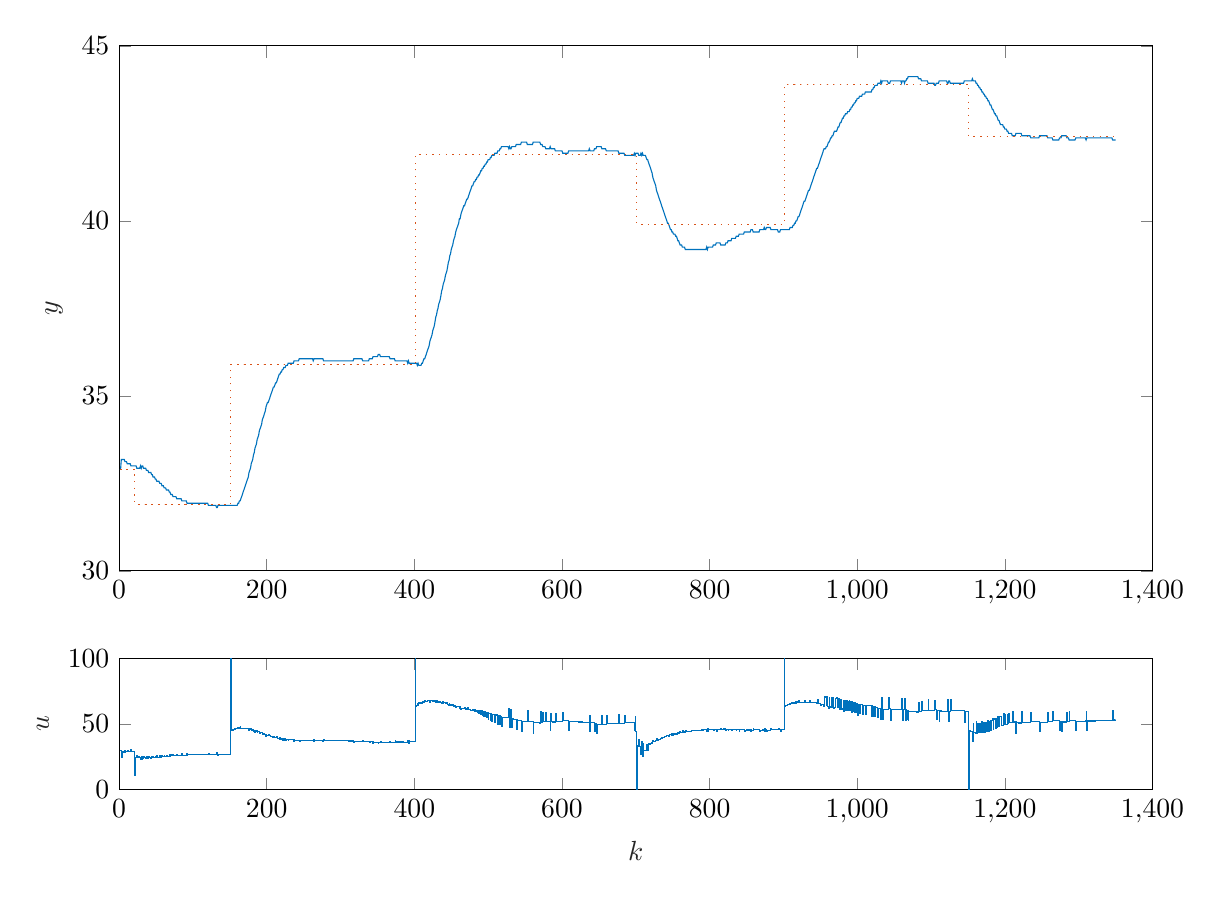
\begin{tikzpicture}

\begin{axis}[%
width=5.167in,
height=0.656in,
at={(0.646in,0.525in)},
scale only axis,
xmin=0,
xmax=1400,
xtick={0,200,400,600,800,1000,1200,1400},
xlabel style={font=\color{white!15!black}},
xlabel={$k$},
ymin=0,
ymax=100,
ytick={0,50,100},
ylabel style={font=\color{white!15!black}},
ylabel={$u$},
axis background/.style={fill=white}
]
\addplot[const plot, color=mycolor1, forget plot] table[row sep=crcr] {%
1	30\\
2	30\\
3	24.7290418658437\\
4	28.7408535975313\\
5	28.7208893292188\\
6	28.7009250609063\\
7	28.6809607925938\\
8	29.7904875530291\\
9	28.9108493422121\\
10	28.8951631313952\\
11	30.0089679493259\\
12	29.1336077960045\\
13	29.1221996426831\\
14	29.1107914893617\\
15	29.0993833360403\\
16	30.2174662114666\\
17	29.3463841156407\\
18	29.3392540198148\\
19	29.3321239239889\\
20	29.3249938281631\\
21	10.4930132532077\\
22	24.8137821991229\\
23	24.7353511450381\\
24	25.9746596244924\\
25	24.8932756374858\\
26	24.8198356504791\\
27	24.7463956634725\\
28	24.6729556764658\\
29	23.2817761559201\\
30	25.5290286353744\\
31	23.1299051148286\\
32	24.0594180607438\\
33	25.2987265401981\\
34	24.2173425531915\\
35	24.1439025661848\\
36	24.0704625791781\\
37	25.1265136209193\\
38	24.1933996914081\\
39	24.124237761897\\
40	25.1845668611336\\
41	24.255730989118\\
42	24.1908471171024\\
43	24.1259632450869\\
44	25.1905704018191\\
45	24.266012587299\\
46	25.523146306318\\
47	24.459587558876\\
48	24.4039728114341\\
49	25.47784909274\\
50	24.5625604027935\\
51	25.6407147415948\\
52	24.729704109144\\
53	24.6826454766931\\
54	24.6355868442423\\
55	25.7180192405392\\
56	24.8112866655838\\
57	24.7685060906285\\
58	26.0434650492122\\
59	24.997731541335\\
60	24.9599420334578\\
61	26.0516435543284\\
62	25.1541801039467\\
63	25.120668653565\\
64	26.216648231931\\
65	25.3234628390449\\
66	25.2942294461588\\
67	25.2649960532726\\
68	26.3652536891343\\
69	25.4763463537436\\
70	26.7691305518921\\
71	25.7412222835796\\
72	25.7212580152671\\
73	26.8307847757024\\
74	25.9511465648854\\
75	25.9354603540685\\
76	25.9197741432515\\
77	25.9040879324346\\
78	27.0178927503653\\
79	26.1425325970439\\
80	26.1311244437225\\
81	26.1197162904011\\
82	26.1083081370797\\
83	26.0968999837582\\
84	26.0854918304368\\
85	27.2035747058632\\
86	26.3324926100373\\
87	26.3253625142114\\
88	26.3182324183855\\
89	26.3111023225596\\
90	26.3039722267337\\
91	26.2968421309078\\
92	27.607451568621\\
93	26.5973685398733\\
94	26.5952295111255\\
95	26.5930904823777\\
96	26.5909514536299\\
97	26.5888124248822\\
98	26.5866733961344\\
99	26.5845343673866\\
100	26.5823953386389\\
101	26.5802563098911\\
102	26.5781172811433\\
103	26.5759782523956\\
104	26.5738392236478\\
105	26.5717001949\\
106	26.5695611661523\\
107	26.5674221374045\\
108	26.5652831086567\\
109	26.563144079909\\
110	26.5610050511612\\
111	26.5588660224134\\
112	26.5567269936657\\
113	26.5545879649179\\
114	26.5524489361701\\
115	26.5503099074224\\
116	26.5481708786746\\
117	26.5460318499268\\
118	26.5438928211791\\
119	26.5417537924313\\
120	26.5396147636835\\
121	27.6669667636835\\
122	26.8051537924313\\
123	26.8072928211791\\
124	26.8094318499268\\
125	26.8115708786746\\
126	26.8137099074224\\
127	26.8158489361701\\
128	26.8179879649179\\
129	26.8201269936657\\
130	26.8222660224134\\
131	26.8244050511612\\
132	27.9560351086568\\
133	27.0985001949\\
134	25.9754262523955\\
135	26.8415172811433\\
136	26.8436563098911\\
137	26.8457953386389\\
138	26.8479343673866\\
139	26.8500733961344\\
140	26.8522124248822\\
141	26.8543514536299\\
142	26.8564904823777\\
143	26.8586295111255\\
144	26.8607685398732\\
145	26.862907568621\\
146	26.8650465973688\\
147	26.8671856261165\\
148	26.8693246548643\\
149	26.8714636836121\\
150	26.8736027123598\\
151	100\\
152	44.8656865194087\\
153	45.1530293811921\\
154	45.4403722429754\\
155	45.7277151047587\\
156	46.0150579665421\\
157	46.3024008283254\\
158	46.5897436901088\\
159	46.8770865518921\\
160	47.1644294136755\\
161	46.3222812467111\\
162	47.4692980509988\\
163	46.4346233217476\\
164	47.7206410589573\\
165	46.8692237674191\\
166	46.8774804183857\\
167	46.8814590118564\\
168	46.6929110430404\\
169	46.8316125119376\\
170	46.8220439233394\\
171	46.8081972772454\\
172	46.6018240688647\\
173	46.7227002981972\\
174	46.6953064700342\\
175	46.6636345843755\\
176	45.3099451076823\\
177	46.2726700399547\\
178	46.2231729147312\\
179	44.8516581984733\\
180	45.7965578911809\\
181	45.7292355263928\\
182	44.3398955705701\\
183	45.266970023713\\
184	43.8640828858211\\
185	44.7776101568946\\
186	44.6789153704728\\
187	43.2582029930161\\
188	44.153905024525\\
189	44.0373849985384\\
190	42.598847381517\\
191	43.4767241734611\\
192	43.3423789079099\\
193	43.2037555848628\\
194	41.7431146707813\\
195	42.5988881656653\\
196	42.4424396030535\\
197	42.093464478155\\
198	42.0717387909697\\
199	40.7722520175411\\
200	41.2694036530779\\
201	41.2298527263278\\
202	42.17152277083\\
203	41.1197497865846\\
204	40.9276507448433\\
205	40.5430251408154\\
206	40.4856489745006\\
207	40.2800027506905\\
208	40.0700784693845\\
209	39.6676276257919\\
210	40.7219172486602\\
211	39.6387718427806\\
212	39.4153003794057\\
213	40.3170418872829\\
214	39.2253403664123\\
215	38.8050642832549\\
216	38.7120376378107\\
217	38.4707409348711\\
218	39.3546572031835\\
219	38.2451304427482\\
220	39.1247686535652\\
221	37.822715330843\\
222	38.8413544745819\\
223	37.7225585895729\\
224	38.5929276758162\\
225	38.5993447620595\\
226	37.4762708195552\\
227	38.3423618483029\\
228	38.3445008770506\\
229	37.2171488770506\\
230	38.0789618483029\\
231	38.0768228195551\\
232	38.0746837908073\\
233	38.0725447620596\\
234	38.0704057333118\\
235	38.068266704564\\
236	38.0661276758163\\
237	36.7462491135294\\
238	37.7470630177035\\
239	37.7399329218776\\
240	37.7328028260518\\
241	37.7256727302259\\
242	37.7185426344\\
243	37.7114125385741\\
244	36.5747914140004\\
245	37.427335260679\\
246	37.4159271073576\\
247	37.4045189540362\\
248	37.3931108007147\\
249	37.3817026473933\\
250	37.3702944940719\\
251	37.3588863407505\\
252	37.347478187429\\
253	37.3360700341076\\
254	37.3246618807862\\
255	37.3132537274648\\
256	37.3018455741434\\
257	37.2904374208219\\
258	37.2790292675005\\
259	37.2676211141791\\
260	37.2562129608577\\
261	37.2448048075362\\
262	37.2333966542148\\
263	38.3514795296412\\
264	36.3509064050675\\
265	37.2034502517461\\
266	37.1920420984247\\
267	37.1806339451032\\
268	37.1692257917818\\
269	37.1578176384604\\
270	37.146409485139\\
271	37.1350013318175\\
272	37.1235931784961\\
273	37.1121850251747\\
274	37.1007768718533\\
275	37.0893687185319\\
276	37.0779605652104\\
277	38.1960434406368\\
278	37.3249613448109\\
279	37.317831248985\\
280	37.3107011531591\\
281	37.3035710573332\\
282	37.2964409615073\\
283	37.2893108656815\\
284	37.2821807698556\\
285	37.2750506740297\\
286	37.2679205782038\\
287	37.2607904823779\\
288	37.253660386552\\
289	37.2465302907261\\
290	37.2394001949002\\
291	37.2322700990743\\
292	37.2251400032484\\
293	37.2180099074226\\
294	37.2108798115967\\
295	37.2037497157708\\
296	37.1966196199449\\
297	37.189489524119\\
298	37.1823594282931\\
299	37.1752293324672\\
300	37.1680992366413\\
301	37.1609691408154\\
302	37.1538390449895\\
303	37.1467089491637\\
304	37.1395788533378\\
305	37.1324487575119\\
306	37.125318661686\\
307	37.1181885658601\\
308	37.1110584700342\\
309	37.1039283742083\\
310	37.0967982783824\\
311	37.0896681825565\\
312	37.0825380867307\\
313	37.0754079909048\\
314	37.0682778950789\\
315	37.061147799253\\
316	37.0540177034271\\
317	37.0468876076012\\
318	35.9102664830275\\
319	36.7628103297061\\
320	36.7514021763847\\
321	36.7399940230633\\
322	36.7285858697418\\
323	36.7171777164204\\
324	36.705769563099\\
325	36.6943614097776\\
326	36.6829532564562\\
327	36.6715451031347\\
328	36.6601369498133\\
329	36.6487287964919\\
330	37.7668116719183\\
331	36.8957295760924\\
332	36.8885994802665\\
333	36.8814693844406\\
334	36.8743392886147\\
335	36.8672091927888\\
336	36.8600790969629\\
337	36.852949001137\\
338	36.8458189053111\\
339	35.7091977807374\\
340	36.561741627416\\
341	36.5503334740946\\
342	36.5389253207732\\
343	36.5275171674518\\
344	35.3866179853827\\
345	36.2348837745656\\
346	36.2191975637487\\
347	36.2035113529317\\
348	36.1878251421148\\
349	36.1721389312978\\
350	36.1564527204809\\
351	35.0112754809161\\
352	35.8552632126036\\
353	35.8352989442911\\
354	36.9448257047265\\
355	36.0651874939095\\
356	36.0495012830925\\
357	36.0338150722756\\
358	36.0181288614586\\
359	36.0024426506417\\
360	35.9867564398247\\
361	35.9710702290077\\
362	35.9553840181908\\
363	35.9396978073738\\
364	35.9240115965569\\
365	35.9083253857399\\
366	35.892639174923\\
367	37.0064439928537\\
368	36.1310838395323\\
369	36.1196756862109\\
370	36.1082675328895\\
371	36.0968593795681\\
372	36.0854512262466\\
373	36.0740430729252\\
374	37.1921259483516\\
375	36.3210438525257\\
376	36.3139137566998\\
377	36.3067836608739\\
378	36.299653565048\\
379	36.2925234692221\\
380	36.2853933733962\\
381	36.2782632775703\\
382	36.2711331817444\\
383	36.2640030859186\\
384	36.2568729900927\\
385	36.2497428942668\\
386	36.2426127984409\\
387	36.235482702615\\
388	36.2283526067891\\
389	36.2212225109632\\
390	36.2140924151373\\
391	37.5247018528505\\
392	35.1968792905637\\
393	37.5154327282768\\
394	36.5053496995291\\
395	36.5032106707813\\
396	36.5010716420336\\
397	36.4989326132858\\
398	36.496793584538\\
399	36.4946545557902\\
400	36.4925155270425\\
401	100\\
402	63.469946093877\\
403	63.8956128146826\\
404	65.450770564236\\
405	63.8872723137893\\
406	66.3063820633428\\
407	65.8723748416438\\
408	66.302319619945\\
409	66.7322643982461\\
410	66.0327181477994\\
411	67.322336868605\\
412	66.4302640558716\\
413	66.7293926808512\\
414	68.0097422770832\\
415	67.2966488445675\\
416	67.443229354556\\
417	67.3972833022579\\
418	67.6785866876728\\
419	67.8116200155924\\
420	67.9403752860162\\
421	66.7471129654055\\
422	67.8702650537604\\
423	67.9811950846195\\
424	67.8995985531919\\
425	67.0157604307297\\
426	67.9728172220241\\
427	67.8733954510318\\
428	66.9717320890049\\
429	66.5932241071955\\
430	67.6671785343516\\
431	66.5994198752644\\
432	67.3282996251426\\
433	66.3909857839862\\
434	67.2945668565864\\
435	67.1416693668999\\
436	66.1865302861788\\
437	65.7545465856753\\
438	66.7750252941372\\
439	65.6537909163559\\
440	66.3291949475398\\
441	66.467896416437\\
442	65.328836799091\\
443	65.9864155907102\\
444	66.1072918200427\\
445	64.9504069631319\\
446	64.4606694864386\\
447	65.423394418711\\
448	64.0561577599485\\
449	65.0053355101515\\
450	63.8128001741113\\
451	64.4169032470364\\
452	64.4843037576746\\
453	63.2739431820697\\
454	63.8602210154301\\
455	63.9097962865036\\
456	62.681610471334\\
457	63.2500630651296\\
458	63.2818130966384\\
459	63.1652930706519\\
460	63.0444949871695\\
461	61.6016793126527\\
462	63.6047690758491\\
463	61.47698078155\\
464	62.0097828962162\\
465	62.0058824485956\\
466	61.8537119434796\\
467	61.6972633808678\\
468	62.6660277895084\\
469	61.4531006646099\\
470	61.4313749774245\\
471	61.2613792327438\\
472	62.2165964593151\\
473	61.1783706571387\\
474	60.8115702926755\\
475	60.7720193659255\\
476	60.58419838168\\
477	60.3920993399388\\
478	60.0074737359109\\
479	61.0795885983439\\
480	60.0142684320291\\
481	59.8086222082189\\
482	60.7281889556608\\
483	59.6543126743549\\
484	60.5696013643013\\
485	58.7853472637546\\
486	60.3416566546226\\
487	58.4345683371998\\
488	60.1401131532008\\
489	57.847419914687\\
490	57.5564344267826\\
491	59.9886950681528\\
492	56.3298099721068\\
493	59.653884885168\\
494	56.1357530640043\\
495	59.3523085342865\\
496	55.4458204241201\\
497	59.023312603324\\
498	54.7278078758549\\
499	58.6655764356825\\
500	53.1205963111708\\
501	58.2009727134587\\
502	58.2195092557466\\
503	53.0788698978755\\
504	57.7949719894726\\
505	52.2632249746871\\
506	57.3375124072936\\
507	57.3415498799007\\
508	57.3455873525077\\
509	51.4220723525074\\
510	56.8538847978259\\
511	56.8496822431442\\
512	56.8454796884625\\
513	49.4029405025187\\
514	56.2281543610669\\
515	56.213503859615\\
516	49.4388929320702\\
517	55.6430776120157\\
518	48.4746076596447\\
519	55.0342263126875\\
520	54.9995740057309\\
521	54.9649216987743\\
522	54.9302693918177\\
523	54.8956170848611\\
524	54.8609647779045\\
525	54.8263124709479\\
526	54.7916601639914\\
527	54.7570078570348\\
528	61.4829763044691\\
529	47.7202353920987\\
530	60.6747097595326\\
531	54.4218825994783\\
532	47.2534126471073\\
533	53.8130313001501\\
534	53.7783789931935\\
535	53.7437266862369\\
536	53.7090743792803\\
537	53.6744220723237\\
538	46.1114327668259\\
539	53.0258250646689\\
540	52.9801813625116\\
541	52.9345376603543\\
542	52.8888939581971\\
543	52.8432502560398\\
544	52.7976065538825\\
545	43.9703153889556\\
546	52.033302761259\\
547	51.9762481335624\\
548	51.9191935058658\\
549	51.8621388781693\\
550	51.8050842504727\\
551	51.7480296227761\\
552	51.6909749950795\\
553	60.4155678301526\\
554	52.2498821279953\\
555	52.2042384258381\\
556	52.1585947236808\\
557	52.1129510215235\\
558	52.0673073193663\\
559	52.021663617209\\
560	51.9760199150517\\
561	43.1487287501247\\
562	51.2117161224282\\
563	51.1546614947316\\
564	51.097606867035\\
565	51.0405522393385\\
566	50.9834976116419\\
567	50.9264429839453\\
568	50.8693883562487\\
569	50.8123337285521\\
570	50.7552791008556\\
571	59.4798719359287\\
572	51.3141862337714\\
573	51.2685425316141\\
574	58.3677078700728\\
575	51.7387846031159\\
576	51.7041322961593\\
577	51.6694799892027\\
578	58.3954484366371\\
579	52.1426212765828\\
580	52.118300036528\\
581	52.0939787964732\\
582	52.0696575564184\\
583	52.0453363163636\\
584	44.8768663639926\\
585	57.8313407314265\\
586	51.5785135713722\\
587	51.5541923313174\\
588	51.5298710912626\\
589	51.5055498512078\\
590	51.481228611153\\
591	57.8333398392658\\
592	51.9559484578137\\
593	51.9412979563619\\
594	51.92664745491\\
595	51.9119969534582\\
596	51.8973464520063\\
597	51.8826959505544\\
598	51.8680454491026\\
599	51.8533949476507\\
600	51.8387444461989\\
601	58.7404064110551\\
602	52.3941863563734\\
603	52.3899838016917\\
604	52.38578124701\\
605	52.3815786923282\\
606	52.3773761376465\\
607	52.3731735829648\\
608	52.3689710282831\\
609	44.9264318423393\\
610	51.7516457008875\\
611	51.7369951994356\\
612	51.7223446979838\\
613	51.7076941965319\\
614	51.6930436950801\\
615	51.6783931936282\\
616	51.6637426921763\\
617	51.6490921907245\\
618	51.6344416892726\\
619	51.6197911878208\\
620	51.6051406863689\\
621	51.590490184917\\
622	51.5758396834652\\
623	51.5611891820133\\
624	51.5465386805614\\
625	51.5318881791096\\
626	51.5172376776577\\
627	51.5025871762059\\
628	51.487936674754\\
629	51.4732861733021\\
630	51.4586356718503\\
631	51.4439851703984\\
632	51.4293346689466\\
633	51.4146841674947\\
634	51.4000336660428\\
635	51.385383164591\\
636	51.3707326631391\\
637	44.5961217355943\\
638	56.8109738437074\\
639	50.9335824622553\\
640	50.9189319608034\\
641	50.9042814593516\\
642	50.8896309578997\\
643	50.8749804564478\\
644	44.100369528903\\
645	50.3045542088485\\
646	50.2802329687937\\
647	43.1117630164227\\
648	49.6713816694655\\
649	49.6367293625089\\
650	49.6020770555523\\
651	49.5674247485957\\
652	49.5327724416391\\
653	49.4981201346825\\
654	56.2240885821169\\
655	49.9712614220626\\
656	49.9469401820078\\
657	49.922618941953\\
658	49.8982977018982\\
659	49.8739764618434\\
660	56.2260876899563\\
661	50.3486963085042\\
662	50.3340458070523\\
663	50.3193953056004\\
664	50.3047448041486\\
665	50.2900943026967\\
666	50.2754438012449\\
667	50.260793299793\\
668	50.2461427983411\\
669	50.2314922968893\\
670	50.2168417954374\\
671	50.2021912939856\\
672	50.1875407925337\\
673	50.1728902910818\\
674	50.15823978963\\
675	50.1435892881781\\
676	50.1289387867263\\
677	57.0306007515825\\
678	50.6843806969008\\
679	50.6801781422191\\
680	50.6759755875374\\
681	50.6717730328556\\
682	50.6675704781739\\
683	50.6633679234922\\
684	50.6591653688105\\
685	56.1989873288107\\
686	51.1327748414175\\
687	51.1368123140245\\
688	51.1408497866315\\
689	51.1448872592385\\
690	51.1489247318455\\
691	51.1529622044525\\
692	51.1569996770595\\
693	51.1610371496665\\
694	51.1650746222735\\
695	51.1691120948805\\
696	51.1731495674875\\
697	51.1771870400946\\
698	45.2536720400943\\
699	55.8637439600947\\
700	44.5042139600943\\
701	0\\
702	33.2615683825588\\
703	32.9771955157623\\
704	38.2478526352955\\
705	32.9124753074352\\
706	32.6473479395752\\
707	26.4436626274601\\
708	36.7845697069935\\
709	25.1448693948782\\
710	35.4857764744116\\
711	30.1503991465513\\
712	29.8852717786913\\
713	29.6201444108313\\
714	34.5258587430761\\
715	34.7272500797355\\
716	30.1599128448517\\
717	34.9928657262756\\
718	34.6013044462495\\
719	34.7988522110233\\
720	34.9938105322994\\
721	35.6387876094393\\
722	35.4888355168876\\
723	37.2385590453121\\
724	36.7321382852017\\
725	36.7624200873781\\
726	36.9409719470499\\
727	37.1238018642175\\
728	38.6286493724195\\
729	37.8170824716561\\
730	38.0177376283883\\
731	38.4109193474073\\
732	38.4768516287132\\
733	38.6910539675144\\
734	38.9095343638114\\
735	39.3205413223951\\
736	39.4042988432657\\
737	39.6363264216317\\
738	39.8726320574934\\
739	40.3014642556418\\
740	40.4030470160772\\
741	40.6528998340078\\
742	40.9070307094343\\
743	41.3536881471474\\
744	40.3436051183997\\
745	41.4709571183997\\
746	41.7386351758951\\
747	42.0105912908863\\
748	41.1573344346251\\
749	42.485769111903\\
750	41.49351132272\\
751	42.6386885622847\\
752	41.7947008305972\\
753	41.8146650989097\\
754	42.9641203959698\\
755	42.1244107217779\\
756	43.2781440763338\\
757	43.7604519931764\\
758	42.786019443558\\
759	43.9490219226875\\
760	44.2523504593124\\
761	43.4304660246852\\
762	43.4725335900579\\
763	44.6440921841785\\
764	43.8264858070468\\
765	43.872831429915\\
766	43.9191770527833\\
767	45.2832622091907\\
768	44.3266548991371\\
769	44.3779915890835\\
770	44.4293282790299\\
771	44.4806649689763\\
772	44.5320016589227\\
773	44.5833383488691\\
774	44.6346750388155\\
775	44.6860117287619\\
776	44.7373484187083\\
777	44.7886851086547\\
778	44.8400217986011\\
779	44.8913584885475\\
780	44.9426951784939\\
781	44.9940318684403\\
782	45.0453685583867\\
783	45.0967052483331\\
784	45.1480419382795\\
785	45.1993786282259\\
786	45.2507153181723\\
787	45.3020520081187\\
788	45.3533886980651\\
789	45.4047253880115\\
790	45.4560620779579\\
791	45.5073987679043\\
792	45.5587354578507\\
793	45.6100721477971\\
794	45.6614088377435\\
795	45.7127455276899\\
796	44.4463426840973\\
797	46.8183718405046\\
798	44.544024996912\\
799	45.5983146197803\\
800	45.6446602426485\\
801	45.6910058655168\\
802	45.7373514883851\\
803	45.7836971112534\\
804	45.8300427341217\\
805	44.7468973282421\\
806	45.6529168936149\\
807	45.6949844589877\\
808	45.7370520243604\\
809	44.6496285609855\\
810	45.5513700688626\\
811	45.5891595767398\\
812	45.6269490846171\\
813	45.6647385924943\\
814	45.7025281003715\\
815	46.8698086369964\\
816	46.0479242023692\\
817	46.0899917677419\\
818	46.1320593331147\\
819	46.1741268984874\\
820	46.2161944638602\\
821	46.2582620292329\\
822	45.170838565858\\
823	46.0725800737351\\
824	46.1103695816124\\
825	45.0186680607418\\
826	45.9161315111235\\
827	45.9496429615051\\
828	45.9831544118868\\
829	46.0166658622685\\
830	44.7324377791111\\
831	45.7689021624147\\
832	45.7974225457182\\
833	45.8259429290218\\
834	45.8544633123254\\
835	45.8829836956289\\
836	44.7820130501847\\
837	45.6702073759927\\
838	45.6944497018008\\
839	45.7186920276088\\
840	44.6134433246691\\
841	45.4973595929815\\
842	45.517323861294\\
843	45.5372881296065\\
844	45.557252397919\\
845	45.5772166662315\\
846	45.597180934544\\
847	44.4876541741087\\
848	45.3672923849257\\
849	45.3829785957426\\
850	45.3986648065596\\
851	45.4143510173765\\
852	45.4300372281935\\
853	45.4457234390104\\
854	45.4614096498274\\
855	45.4770958606443\\
856	44.1750425379222\\
857	45.1936816816611\\
858	45.2043768253999\\
859	46.5328115026778\\
860	45.5405537134948\\
861	45.5562399243117\\
862	45.5719261351287\\
863	45.5876123459456\\
864	45.6032985567626\\
865	45.6189847675795\\
866	45.6346709783965\\
867	45.6503571892135\\
868	44.3483038664913\\
869	45.3669430102302\\
870	45.377638153969\\
871	45.3883332977078\\
872	45.3990284414467\\
873	45.4097235851855\\
874	44.2909277001765\\
875	46.2907878151677\\
876	45.4375309589065\\
877	44.3187350738975\\
878	45.1891041601408\\
879	45.1955212463841\\
880	45.2019383326274\\
881	45.2083554188707\\
882	45.214772505114\\
883	46.3506806201052\\
884	45.497423763844\\
885	45.5081189075828\\
886	45.5188140513216\\
887	45.5295091950605\\
888	45.5402043387993\\
889	45.5508994825381\\
890	45.561594626277\\
891	45.5722897700158\\
892	45.5829849137546\\
893	46.9114195910325\\
894	45.9191618018495\\
895	45.9348480126664\\
896	44.6327946899443\\
897	45.6514338336832\\
898	45.662128977422\\
899	45.6728241211608\\
900	45.6835192648997\\
901	100\\
902	63.6927153019307\\
903	63.9886142787051\\
904	64.2845132554795\\
905	64.5804122322539\\
906	64.8763112090283\\
907	65.1722101858027\\
908	65.4681091625771\\
909	64.6345171106037\\
910	65.7900900298825\\
911	66.0817109491614\\
912	66.3733318684403\\
913	65.5354617589715\\
914	66.6867566207548\\
915	65.8446084537903\\
916	66.9916252580781\\
917	65.9569505288269\\
918	67.2429682660366\\
919	66.3915509744984\\
920	66.3998076254649\\
921	67.5332772476835\\
922	66.6733038411543\\
923	66.4847558723383\\
924	66.6234573412355\\
925	66.6138887526373\\
926	66.6000421065433\\
927	66.3936688981626\\
928	66.5145451274951\\
929	67.6166423280798\\
930	66.7252964999169\\
931	66.6936246142581\\
932	66.4694261663127\\
933	66.5724771560804\\
934	66.5272580883528\\
935	67.6072519918771\\
936	66.6938028666538\\
937	66.4517791791437\\
938	66.5370049293467\\
939	66.4739606220543\\
940	66.4066382572661\\
941	66.0685036701596\\
942	66.2603791978247\\
943	66.1673464960467\\
944	66.0648190565257\\
945	65.4219306057857\\
946	68.9473032841527\\
947	65.6414746999426\\
948	65.5045242583776\\
949	65.3553277111574\\
950	64.3962213638174\\
951	65.0023071147657\\
952	64.8099749004474\\
953	64.6026452125616\\
954	63.3158569356552\\
955	64.1118517487954\\
956	70.6200519294258\\
957	70.899746190056\\
958	64.0462972100177\\
959	70.9209368353933\\
960	63.6839739738759\\
961	62.1427452529297\\
962	70.5317590692136\\
963	63.2736044888375\\
964	62.9657051151431\\
965	70.1751513447876\\
966	62.8974351777727\\
967	70.0971006140986\\
968	61.5550825876546\\
969	62.3762167017809\\
970	69.5546904192481\\
971	69.7731281367151\\
972	69.991565854182\\
973	62.6828771749898\\
974	62.3244437024768\\
975	69.4833558333051\\
976	60.9005845013635\\
977	61.6809653099923\\
978	68.818685721962\\
979	61.4692437372723\\
980	61.0700569592617\\
981	68.1882157845925\\
982	59.5646911471533\\
983	67.8314450469446\\
984	60.4510305500758\\
985	67.5479976565478\\
986	67.6849287630196\\
987	60.2947334728323\\
988	67.3819197859842\\
989	67.5090700991366\\
990	60.109094015629\\
991	67.1864995354622\\
992	58.5222215925255\\
993	66.7482221868192\\
994	59.3270543844528\\
995	66.3832681854273\\
996	58.9523195897425\\
997	65.9987525973967\\
998	58.5580232083916\\
999	65.5946754227272\\
1000	56.889644174293\\
1001	65.0748914630891\\
1002	65.1400967518852\\
1003	57.6781756440213\\
1004	64.6936361394983\\
1005	64.7490606349749\\
1006	64.8044851304516\\
1007	57.3327832292692\\
1008	64.3384629314259\\
1009	64.3841066335832\\
1010	64.4297503357405\\
1011	56.9482676412377\\
1012	63.9441665500759\\
1013	63.9800294589137\\
1014	64.0158923677516\\
1015	64.0517552765894\\
1016	64.0876181854273\\
1017	64.1234810942651\\
1018	64.159344003103\\
1019	64.1952069119409\\
1020	55.449422358009\\
1021	63.5939163413076\\
1022	56.0912419279461\\
1023	63.0659491179255\\
1024	55.5534939112455\\
1025	62.5184203079047\\
1026	62.5233107045644\\
1027	62.5282011012241\\
1028	55.0059651012238\\
1029	61.9611107045644\\
1030	61.9562203079047\\
1031	61.951329911245\\
1032	53.1647920518156\\
1033	70.0501801923863\\
1034	53.1436003329568\\
1035	61.2473410107578\\
1036	61.2310396885588\\
1037	61.2147383663598\\
1038	61.1984370441608\\
1039	61.1821357219617\\
1040	61.1658343997627\\
1041	61.1495330775637\\
1042	69.9148792181344\\
1043	61.7899468214746\\
1044	61.7850564248149\\
1045	52.9985185653855\\
1046	61.1022592431865\\
1047	61.0859579209875\\
1048	61.0696565987885\\
1049	61.0533552765894\\
1050	61.0370539543904\\
1051	61.0207526321914\\
1052	61.0044513099924\\
1053	60.9881499877933\\
1054	60.9718486655943\\
1055	60.9555473433953\\
1056	60.9392460211963\\
1057	60.9229446989973\\
1058	60.9066433767982\\
1059	60.8903420545992\\
1060	69.6556881951699\\
1061	52.7491083357404\\
1062	60.8528490135414\\
1063	60.8365476913424\\
1064	69.6018938319131\\
1065	52.6953139724837\\
1066	60.7990546502847\\
1067	53.2556269314256\\
1068	60.1895808159075\\
1069	52.6363723037299\\
1070	59.5605453948915\\
1071	59.5246824860537\\
1072	59.4888195772158\\
1073	59.452956668378\\
1074	59.4170937595401\\
1075	59.3812308507023\\
1076	59.3453679418644\\
1077	59.3095050330265\\
1078	59.2736421241887\\
1079	59.2377792153508\\
1080	59.201916306513\\
1081	59.1660533976751\\
1082	59.1301904888373\\
1083	66.6214539766585\\
1084	59.6353358611406\\
1085	59.6092537456222\\
1086	59.5831716301038\\
1087	67.0842159112453\\
1088	60.107878589046\\
1089	60.091577266847\\
1090	60.075275944648\\
1091	60.058974622449\\
1092	60.0426733002499\\
1093	60.0263719780509\\
1094	60.0100706558519\\
1095	59.9937693336529\\
1096	68.7591154742235\\
1097	60.6341830775638\\
1098	60.6292926809041\\
1099	60.6244022842444\\
1100	60.6195118875847\\
1101	60.614621490925\\
1102	60.6097310942653\\
1103	60.6048406976056\\
1104	60.5999503009458\\
1105	68.1221863009461\\
1106	61.1670406976056\\
1107	53.6448046976053\\
1108	60.5999503009458\\
1109	60.5950599042861\\
1110	60.5901695076264\\
1111	51.803631648197\\
1112	59.907372325998\\
1113	59.891071003799\\
1114	59.8747696816\\
1115	59.858468359401\\
1116	59.8421670372019\\
1117	59.8258657150029\\
1118	59.8095643928039\\
1119	59.7932630706049\\
1120	59.7769617484058\\
1121	59.7606604262068\\
1122	68.5260065667775\\
1123	60.4010741701178\\
1124	51.6145363106884\\
1125	59.7182769884894\\
1126	68.48362312906\\
1127	60.3586907324003\\
1128	60.3538003357406\\
1129	60.3489099390809\\
1130	60.3440195424212\\
1131	60.3391291457615\\
1132	60.3342387491018\\
1133	60.3293483524421\\
1134	60.3244579557823\\
1135	60.3195675591226\\
1136	60.3146771624629\\
1137	60.3097867658032\\
1138	60.3048963691435\\
1139	60.3000059724838\\
1140	60.2951155758241\\
1141	60.2902251791644\\
1142	60.2853347825047\\
1143	60.280444385845\\
1144	60.2755539891853\\
1145	51.4890161297559\\
1146	59.5927568075569\\
1147	59.5764554853579\\
1148	59.5601541631588\\
1149	59.5438528409598\\
1150	59.5275515187608\\
1151	0\\
1152	45.0731691248847\\
1153	44.8123479697003\\
1154	44.5515268145159\\
1155	44.2907056593315\\
1156	36.5027581074871\\
1157	50.7193185556436\\
1158	43.4984614004589\\
1159	43.2376402452745\\
1160	42.9768190900901\\
1161	51.4976453976754\\
1162	43.1281931680302\\
1163	50.4059093350452\\
1164	43.2062438987193\\
1165	50.4937408590527\\
1166	43.3038562160471\\
1167	50.6011339697008\\
1168	43.4210301200137\\
1169	51.9826097330965\\
1170	43.653910808949\\
1171	50.9723802814615\\
1172	43.8134681506331\\
1173	51.1417184164641\\
1174	43.992587078956\\
1175	51.3306181381073\\
1176	44.1912675939178\\
1177	52.7936005124982\\
1178	44.5056548938482\\
1179	51.8648776718583\\
1180	52.2738452431866\\
1181	45.165467211176\\
1182	52.5442515758249\\
1183	54.2273017999026\\
1184	45.9801094867502\\
1185	53.3800855702578\\
1186	53.8298064470837\\
1187	46.7621817205707\\
1188	54.1817193907171\\
1189	47.1238754575227\\
1190	55.8077149870982\\
1191	55.1284023761033\\
1192	48.0917501617677\\
1193	55.5422603440914\\
1194	56.0425153197359\\
1195	49.0254246920391\\
1196	48.9683700643425\\
1197	48.9113154366459\\
1198	57.635908271719\\
1199	49.4702225695617\\
1200	56.9517052640645\\
1201	49.9558063552263\\
1202	49.9199434463885\\
1203	57.4112069342097\\
1204	50.4250888186918\\
1205	57.9261330998334\\
1206	50.9497957776341\\
1207	50.9334944554351\\
1208	50.9171931332361\\
1209	50.900891811037\\
1210	59.6662379516077\\
1211	51.541305554948\\
1212	51.5364151582883\\
1213	51.5315247616286\\
1214	51.5266343649689\\
1215	42.7400965055395\\
1216	50.8438371833405\\
1217	50.8275358611414\\
1218	50.8112345389424\\
1219	50.7949332167434\\
1220	50.7786318945444\\
1221	50.7623305723453\\
1222	50.7460292501463\\
1223	59.511375390717\\
1224	51.3864429940572\\
1225	51.3815525973975\\
1226	51.3766622007378\\
1227	51.3717718040781\\
1228	51.3668814074184\\
1229	51.3619910107587\\
1230	51.357100614099\\
1231	51.3522102174393\\
1232	51.3473198207796\\
1233	51.3424294241199\\
1234	51.3375390274602\\
1235	58.8597750274605\\
1236	51.9046294241199\\
1237	51.9095198207796\\
1238	51.9144102174393\\
1239	51.919300614099\\
1240	51.9241910107587\\
1241	51.9290814074184\\
1242	51.9339718040781\\
1243	51.9388622007379\\
1244	51.9437525973976\\
1245	51.9486429940573\\
1246	51.953533390717\\
1247	44.4312973907167\\
1248	51.3864429940572\\
1249	51.3815525973975\\
1250	51.3766622007378\\
1251	51.3717718040781\\
1252	51.3668814074184\\
1253	51.3619910107587\\
1254	51.357100614099\\
1255	51.3522102174393\\
1256	51.3473198207796\\
1257	51.3424294241199\\
1258	58.8646654241202\\
1259	51.9095198207796\\
1260	51.9144102174393\\
1261	51.919300614099\\
1262	51.9241910107587\\
1263	51.9290814074184\\
1264	51.9339718040781\\
1265	59.465988597397\\
1266	52.5206237873766\\
1267	52.5352949773557\\
1268	52.5499661673349\\
1269	52.564637357314\\
1270	52.5793085472931\\
1271	52.5939797372722\\
1272	52.6086509272513\\
1273	52.6233221172305\\
1274	45.1108669105505\\
1275	52.0757933072096\\
1276	52.0806837038693\\
1277	44.558447703869\\
1278	51.5135933072096\\
1279	51.5087029105499\\
1280	51.5038125138902\\
1281	51.4989221172305\\
1282	51.4940317205708\\
1283	51.4891413239111\\
1284	59.0113773239113\\
1285	52.0562317205708\\
1286	52.0611221172305\\
1287	59.5931389105493\\
1288	52.647774100529\\
1289	52.6624452905081\\
1290	52.6771164804872\\
1291	52.6917876704663\\
1292	52.7064588604455\\
1293	52.7211300504246\\
1294	52.7358012404037\\
1295	52.7504724303828\\
1296	45.2380172237028\\
1297	52.202943620362\\
1298	52.2078340170217\\
1299	52.2127244136814\\
1300	52.2176148103411\\
1301	52.2225052070008\\
1302	52.2273956036605\\
1303	52.2322860003202\\
1304	52.2371763969799\\
1305	52.2420667936396\\
1306	52.2469571902993\\
1307	52.2518475869591\\
1308	52.2567379836188\\
1309	52.2616283802785\\
1310	59.7936451735973\\
1311	45.3211539669179\\
1312	52.286080363577\\
1313	52.2909707602367\\
1314	52.2958611568964\\
1315	52.3007515535561\\
1316	52.3056419502158\\
1317	52.3105323468755\\
1318	52.3154227435353\\
1319	52.320313140195\\
1320	52.3252035368547\\
1321	52.3300939335144\\
1322	52.3349843301741\\
1323	52.3398747268338\\
1324	52.3447651234935\\
1325	52.3496555201532\\
1326	52.3545459168129\\
1327	52.3594363134726\\
1328	52.3643267101323\\
1329	52.369217106792\\
1330	52.3741075034517\\
1331	52.3789979001114\\
1332	52.3838882967711\\
1333	52.3887786934309\\
1334	52.3936690900906\\
1335	52.3985594867503\\
1336	52.40344988341\\
1337	52.4083402800697\\
1338	52.4132306767294\\
1339	52.4181210733891\\
1340	52.4230114700488\\
1341	52.4279018667085\\
1342	52.4327922633682\\
1343	52.4376826600279\\
1344	52.4425730566876\\
1345	52.4474634533473\\
1346	59.9794802466662\\
1347	53.0341154366458\\
1348	53.048786626625\\
1349	53.0634578166041\\
1350	53.0781290065832\\
};
\end{axis}

\begin{axis}[%
width=5.167in,
height=2.625in,
at={(0.646in,1.619in)},
scale only axis,
xmin=0,
xmax=1400,
xtick={0,200,400,600,800,1000,1200,1400},
ymin=30,
ymax=45,
ytick={30,35,40,45},
ylabel style={font=\color{white!15!black}},
ylabel={$y$},
axis background/.style={fill=white}
]
\addplot [color=mycolor1, forget plot]
  table[row sep=crcr]{%
1	32.9\\
2	32.9\\
3	33.18\\
4	33.18\\
5	33.18\\
6	33.18\\
7	33.18\\
8	33.12\\
9	33.12\\
10	33.12\\
11	33.06\\
12	33.06\\
13	33.06\\
14	33.06\\
15	33.06\\
16	33\\
17	33\\
18	33\\
19	33\\
20	33\\
21	33\\
22	33\\
23	33\\
24	32.93\\
25	32.93\\
26	32.93\\
27	32.93\\
28	32.93\\
29	33\\
30	32.93\\
31	33\\
32	33\\
33	32.93\\
34	32.93\\
35	32.93\\
36	32.93\\
37	32.87\\
38	32.87\\
39	32.87\\
40	32.81\\
41	32.81\\
42	32.81\\
43	32.81\\
44	32.75\\
45	32.75\\
46	32.68\\
47	32.68\\
48	32.68\\
49	32.62\\
50	32.62\\
51	32.56\\
52	32.56\\
53	32.56\\
54	32.56\\
55	32.5\\
56	32.5\\
57	32.5\\
58	32.43\\
59	32.43\\
60	32.43\\
61	32.37\\
62	32.37\\
63	32.37\\
64	32.31\\
65	32.31\\
66	32.31\\
67	32.31\\
68	32.25\\
69	32.25\\
70	32.18\\
71	32.18\\
72	32.18\\
73	32.12\\
74	32.12\\
75	32.12\\
76	32.12\\
77	32.12\\
78	32.06\\
79	32.06\\
80	32.06\\
81	32.06\\
82	32.06\\
83	32.06\\
84	32.06\\
85	32\\
86	32\\
87	32\\
88	32\\
89	32\\
90	32\\
91	32\\
92	31.93\\
93	31.93\\
94	31.93\\
95	31.93\\
96	31.93\\
97	31.93\\
98	31.93\\
99	31.93\\
100	31.93\\
101	31.93\\
102	31.93\\
103	31.93\\
104	31.93\\
105	31.93\\
106	31.93\\
107	31.93\\
108	31.93\\
109	31.93\\
110	31.93\\
111	31.93\\
112	31.93\\
113	31.93\\
114	31.93\\
115	31.93\\
116	31.93\\
117	31.93\\
118	31.93\\
119	31.93\\
120	31.93\\
121	31.87\\
122	31.87\\
123	31.87\\
124	31.87\\
125	31.87\\
126	31.87\\
127	31.87\\
128	31.87\\
129	31.87\\
130	31.87\\
131	31.87\\
132	31.81\\
133	31.81\\
134	31.87\\
135	31.87\\
136	31.87\\
137	31.87\\
138	31.87\\
139	31.87\\
140	31.87\\
141	31.87\\
142	31.87\\
143	31.87\\
144	31.87\\
145	31.87\\
146	31.87\\
147	31.87\\
148	31.87\\
149	31.87\\
150	31.87\\
151	31.87\\
152	31.87\\
153	31.87\\
154	31.87\\
155	31.87\\
156	31.87\\
157	31.87\\
158	31.87\\
159	31.87\\
160	31.87\\
161	31.93\\
162	31.93\\
163	32\\
164	32\\
165	32.06\\
166	32.12\\
167	32.18\\
168	32.25\\
169	32.31\\
170	32.37\\
171	32.43\\
172	32.5\\
173	32.56\\
174	32.62\\
175	32.68\\
176	32.81\\
177	32.87\\
178	32.93\\
179	33.06\\
180	33.12\\
181	33.18\\
182	33.31\\
183	33.37\\
184	33.5\\
185	33.56\\
186	33.62\\
187	33.75\\
188	33.81\\
189	33.87\\
190	34\\
191	34.06\\
192	34.12\\
193	34.18\\
194	34.31\\
195	34.37\\
196	34.43\\
197	34.5\\
198	34.56\\
199	34.68\\
200	34.75\\
201	34.81\\
202	34.81\\
203	34.87\\
204	34.93\\
205	35\\
206	35.06\\
207	35.12\\
208	35.18\\
209	35.25\\
210	35.25\\
211	35.31\\
212	35.37\\
213	35.37\\
214	35.43\\
215	35.5\\
216	35.56\\
217	35.62\\
218	35.62\\
219	35.68\\
220	35.68\\
221	35.75\\
222	35.75\\
223	35.81\\
224	35.81\\
225	35.81\\
226	35.87\\
227	35.87\\
228	35.87\\
229	35.93\\
230	35.93\\
231	35.93\\
232	35.93\\
233	35.93\\
234	35.93\\
235	35.93\\
236	35.93\\
237	36\\
238	36\\
239	36\\
240	36\\
241	36\\
242	36\\
243	36\\
244	36.06\\
245	36.06\\
246	36.06\\
247	36.06\\
248	36.06\\
249	36.06\\
250	36.06\\
251	36.06\\
252	36.06\\
253	36.06\\
254	36.06\\
255	36.06\\
256	36.06\\
257	36.06\\
258	36.06\\
259	36.06\\
260	36.06\\
261	36.06\\
262	36.06\\
263	36\\
264	36.06\\
265	36.06\\
266	36.06\\
267	36.06\\
268	36.06\\
269	36.06\\
270	36.06\\
271	36.06\\
272	36.06\\
273	36.06\\
274	36.06\\
275	36.06\\
276	36.06\\
277	36\\
278	36\\
279	36\\
280	36\\
281	36\\
282	36\\
283	36\\
284	36\\
285	36\\
286	36\\
287	36\\
288	36\\
289	36\\
290	36\\
291	36\\
292	36\\
293	36\\
294	36\\
295	36\\
296	36\\
297	36\\
298	36\\
299	36\\
300	36\\
301	36\\
302	36\\
303	36\\
304	36\\
305	36\\
306	36\\
307	36\\
308	36\\
309	36\\
310	36\\
311	36\\
312	36\\
313	36\\
314	36\\
315	36\\
316	36\\
317	36\\
318	36.06\\
319	36.06\\
320	36.06\\
321	36.06\\
322	36.06\\
323	36.06\\
324	36.06\\
325	36.06\\
326	36.06\\
327	36.06\\
328	36.06\\
329	36.06\\
330	36\\
331	36\\
332	36\\
333	36\\
334	36\\
335	36\\
336	36\\
337	36\\
338	36\\
339	36.06\\
340	36.06\\
341	36.06\\
342	36.06\\
343	36.06\\
344	36.12\\
345	36.12\\
346	36.12\\
347	36.12\\
348	36.12\\
349	36.12\\
350	36.12\\
351	36.18\\
352	36.18\\
353	36.18\\
354	36.12\\
355	36.12\\
356	36.12\\
357	36.12\\
358	36.12\\
359	36.12\\
360	36.12\\
361	36.12\\
362	36.12\\
363	36.12\\
364	36.12\\
365	36.12\\
366	36.12\\
367	36.06\\
368	36.06\\
369	36.06\\
370	36.06\\
371	36.06\\
372	36.06\\
373	36.06\\
374	36\\
375	36\\
376	36\\
377	36\\
378	36\\
379	36\\
380	36\\
381	36\\
382	36\\
383	36\\
384	36\\
385	36\\
386	36\\
387	36\\
388	36\\
389	36\\
390	36\\
391	35.93\\
392	36\\
393	35.93\\
394	35.93\\
395	35.93\\
396	35.93\\
397	35.93\\
398	35.93\\
399	35.93\\
400	35.93\\
401	35.93\\
402	35.93\\
403	35.93\\
404	35.87\\
405	35.93\\
406	35.87\\
407	35.87\\
408	35.87\\
409	35.87\\
410	35.93\\
411	35.93\\
412	36\\
413	36.06\\
414	36.06\\
415	36.12\\
416	36.18\\
417	36.25\\
418	36.31\\
419	36.37\\
420	36.43\\
421	36.56\\
422	36.62\\
423	36.68\\
424	36.75\\
425	36.87\\
426	36.93\\
427	37\\
428	37.12\\
429	37.25\\
430	37.31\\
431	37.43\\
432	37.5\\
433	37.62\\
434	37.68\\
435	37.75\\
436	37.87\\
437	38\\
438	38.06\\
439	38.18\\
440	38.25\\
441	38.31\\
442	38.43\\
443	38.5\\
444	38.56\\
445	38.68\\
446	38.81\\
447	38.87\\
448	39\\
449	39.06\\
450	39.18\\
451	39.25\\
452	39.31\\
453	39.43\\
454	39.5\\
455	39.56\\
456	39.68\\
457	39.75\\
458	39.81\\
459	39.87\\
460	39.93\\
461	40.06\\
462	40.06\\
463	40.18\\
464	40.25\\
465	40.31\\
466	40.37\\
467	40.43\\
468	40.43\\
469	40.5\\
470	40.56\\
471	40.62\\
472	40.62\\
473	40.68\\
474	40.75\\
475	40.81\\
476	40.87\\
477	40.93\\
478	41\\
479	41\\
480	41.06\\
481	41.12\\
482	41.12\\
483	41.18\\
484	41.18\\
485	41.25\\
486	41.25\\
487	41.31\\
488	41.31\\
489	41.37\\
490	41.43\\
491	41.43\\
492	41.5\\
493	41.5\\
494	41.56\\
495	41.56\\
496	41.62\\
497	41.62\\
498	41.68\\
499	41.68\\
500	41.75\\
501	41.75\\
502	41.75\\
503	41.81\\
504	41.81\\
505	41.87\\
506	41.87\\
507	41.87\\
508	41.87\\
509	41.93\\
510	41.93\\
511	41.93\\
512	41.93\\
513	42\\
514	42\\
515	42\\
516	42.06\\
517	42.06\\
518	42.12\\
519	42.12\\
520	42.12\\
521	42.12\\
522	42.12\\
523	42.12\\
524	42.12\\
525	42.12\\
526	42.12\\
527	42.12\\
528	42.06\\
529	42.12\\
530	42.06\\
531	42.06\\
532	42.12\\
533	42.12\\
534	42.12\\
535	42.12\\
536	42.12\\
537	42.12\\
538	42.18\\
539	42.18\\
540	42.18\\
541	42.18\\
542	42.18\\
543	42.18\\
544	42.18\\
545	42.25\\
546	42.25\\
547	42.25\\
548	42.25\\
549	42.25\\
550	42.25\\
551	42.25\\
552	42.25\\
553	42.18\\
554	42.18\\
555	42.18\\
556	42.18\\
557	42.18\\
558	42.18\\
559	42.18\\
560	42.18\\
561	42.25\\
562	42.25\\
563	42.25\\
564	42.25\\
565	42.25\\
566	42.25\\
567	42.25\\
568	42.25\\
569	42.25\\
570	42.25\\
571	42.18\\
572	42.18\\
573	42.18\\
574	42.12\\
575	42.12\\
576	42.12\\
577	42.12\\
578	42.06\\
579	42.06\\
580	42.06\\
581	42.06\\
582	42.06\\
583	42.06\\
584	42.12\\
585	42.06\\
586	42.06\\
587	42.06\\
588	42.06\\
589	42.06\\
590	42.06\\
591	42\\
592	42\\
593	42\\
594	42\\
595	42\\
596	42\\
597	42\\
598	42\\
599	42\\
600	42\\
601	41.93\\
602	41.93\\
603	41.93\\
604	41.93\\
605	41.93\\
606	41.93\\
607	41.93\\
608	41.93\\
609	42\\
610	42\\
611	42\\
612	42\\
613	42\\
614	42\\
615	42\\
616	42\\
617	42\\
618	42\\
619	42\\
620	42\\
621	42\\
622	42\\
623	42\\
624	42\\
625	42\\
626	42\\
627	42\\
628	42\\
629	42\\
630	42\\
631	42\\
632	42\\
633	42\\
634	42\\
635	42\\
636	42\\
637	42.06\\
638	42\\
639	42\\
640	42\\
641	42\\
642	42\\
643	42\\
644	42.06\\
645	42.06\\
646	42.06\\
647	42.12\\
648	42.12\\
649	42.12\\
650	42.12\\
651	42.12\\
652	42.12\\
653	42.12\\
654	42.06\\
655	42.06\\
656	42.06\\
657	42.06\\
658	42.06\\
659	42.06\\
660	42\\
661	42\\
662	42\\
663	42\\
664	42\\
665	42\\
666	42\\
667	42\\
668	42\\
669	42\\
670	42\\
671	42\\
672	42\\
673	42\\
674	42\\
675	42\\
676	42\\
677	41.93\\
678	41.93\\
679	41.93\\
680	41.93\\
681	41.93\\
682	41.93\\
683	41.93\\
684	41.93\\
685	41.87\\
686	41.87\\
687	41.87\\
688	41.87\\
689	41.87\\
690	41.87\\
691	41.87\\
692	41.87\\
693	41.87\\
694	41.87\\
695	41.87\\
696	41.87\\
697	41.87\\
698	41.93\\
699	41.87\\
700	41.93\\
701	41.93\\
702	41.93\\
703	41.93\\
704	41.87\\
705	41.87\\
706	41.87\\
707	41.93\\
708	41.87\\
709	41.93\\
710	41.87\\
711	41.87\\
712	41.87\\
713	41.87\\
714	41.81\\
715	41.75\\
716	41.75\\
717	41.68\\
718	41.62\\
719	41.56\\
720	41.5\\
721	41.43\\
722	41.37\\
723	41.25\\
724	41.18\\
725	41.12\\
726	41.06\\
727	41\\
728	40.87\\
729	40.81\\
730	40.75\\
731	40.68\\
732	40.62\\
733	40.56\\
734	40.5\\
735	40.43\\
736	40.37\\
737	40.31\\
738	40.25\\
739	40.18\\
740	40.12\\
741	40.06\\
742	40\\
743	39.93\\
744	39.93\\
745	39.87\\
746	39.81\\
747	39.75\\
748	39.75\\
749	39.68\\
750	39.68\\
751	39.62\\
752	39.62\\
753	39.62\\
754	39.56\\
755	39.56\\
756	39.5\\
757	39.43\\
758	39.43\\
759	39.37\\
760	39.31\\
761	39.31\\
762	39.31\\
763	39.25\\
764	39.25\\
765	39.25\\
766	39.25\\
767	39.18\\
768	39.18\\
769	39.18\\
770	39.18\\
771	39.18\\
772	39.18\\
773	39.18\\
774	39.18\\
775	39.18\\
776	39.18\\
777	39.18\\
778	39.18\\
779	39.18\\
780	39.18\\
781	39.18\\
782	39.18\\
783	39.18\\
784	39.18\\
785	39.18\\
786	39.18\\
787	39.18\\
788	39.18\\
789	39.18\\
790	39.18\\
791	39.18\\
792	39.18\\
793	39.18\\
794	39.18\\
795	39.18\\
796	39.25\\
797	39.18\\
798	39.25\\
799	39.25\\
800	39.25\\
801	39.25\\
802	39.25\\
803	39.25\\
804	39.25\\
805	39.31\\
806	39.31\\
807	39.31\\
808	39.31\\
809	39.37\\
810	39.37\\
811	39.37\\
812	39.37\\
813	39.37\\
814	39.37\\
815	39.31\\
816	39.31\\
817	39.31\\
818	39.31\\
819	39.31\\
820	39.31\\
821	39.31\\
822	39.37\\
823	39.37\\
824	39.37\\
825	39.43\\
826	39.43\\
827	39.43\\
828	39.43\\
829	39.43\\
830	39.5\\
831	39.5\\
832	39.5\\
833	39.5\\
834	39.5\\
835	39.5\\
836	39.56\\
837	39.56\\
838	39.56\\
839	39.56\\
840	39.62\\
841	39.62\\
842	39.62\\
843	39.62\\
844	39.62\\
845	39.62\\
846	39.62\\
847	39.68\\
848	39.68\\
849	39.68\\
850	39.68\\
851	39.68\\
852	39.68\\
853	39.68\\
854	39.68\\
855	39.68\\
856	39.75\\
857	39.75\\
858	39.75\\
859	39.68\\
860	39.68\\
861	39.68\\
862	39.68\\
863	39.68\\
864	39.68\\
865	39.68\\
866	39.68\\
867	39.68\\
868	39.75\\
869	39.75\\
870	39.75\\
871	39.75\\
872	39.75\\
873	39.75\\
874	39.81\\
875	39.75\\
876	39.75\\
877	39.81\\
878	39.81\\
879	39.81\\
880	39.81\\
881	39.81\\
882	39.81\\
883	39.75\\
884	39.75\\
885	39.75\\
886	39.75\\
887	39.75\\
888	39.75\\
889	39.75\\
890	39.75\\
891	39.75\\
892	39.75\\
893	39.68\\
894	39.68\\
895	39.68\\
896	39.75\\
897	39.75\\
898	39.75\\
899	39.75\\
900	39.75\\
901	39.75\\
902	39.75\\
903	39.75\\
904	39.75\\
905	39.75\\
906	39.75\\
907	39.75\\
908	39.75\\
909	39.81\\
910	39.81\\
911	39.81\\
912	39.81\\
913	39.87\\
914	39.87\\
915	39.93\\
916	39.93\\
917	40\\
918	40\\
919	40.06\\
920	40.12\\
921	40.12\\
922	40.18\\
923	40.25\\
924	40.31\\
925	40.37\\
926	40.43\\
927	40.5\\
928	40.56\\
929	40.56\\
930	40.62\\
931	40.68\\
932	40.75\\
933	40.81\\
934	40.87\\
935	40.87\\
936	40.93\\
937	41\\
938	41.06\\
939	41.12\\
940	41.18\\
941	41.25\\
942	41.31\\
943	41.37\\
944	41.43\\
945	41.5\\
946	41.5\\
947	41.56\\
948	41.62\\
949	41.68\\
950	41.75\\
951	41.81\\
952	41.87\\
953	41.93\\
954	42\\
955	42.06\\
956	42.06\\
957	42.06\\
958	42.12\\
959	42.12\\
960	42.18\\
961	42.25\\
962	42.25\\
963	42.31\\
964	42.37\\
965	42.37\\
966	42.43\\
967	42.43\\
968	42.5\\
969	42.56\\
970	42.56\\
971	42.56\\
972	42.56\\
973	42.62\\
974	42.68\\
975	42.68\\
976	42.75\\
977	42.81\\
978	42.81\\
979	42.87\\
980	42.93\\
981	42.93\\
982	43\\
983	43\\
984	43.06\\
985	43.06\\
986	43.06\\
987	43.12\\
988	43.12\\
989	43.12\\
990	43.18\\
991	43.18\\
992	43.25\\
993	43.25\\
994	43.31\\
995	43.31\\
996	43.37\\
997	43.37\\
998	43.43\\
999	43.43\\
1000	43.5\\
1001	43.5\\
1002	43.5\\
1003	43.56\\
1004	43.56\\
1005	43.56\\
1006	43.56\\
1007	43.62\\
1008	43.62\\
1009	43.62\\
1010	43.62\\
1011	43.68\\
1012	43.68\\
1013	43.68\\
1014	43.68\\
1015	43.68\\
1016	43.68\\
1017	43.68\\
1018	43.68\\
1019	43.68\\
1020	43.75\\
1021	43.75\\
1022	43.81\\
1023	43.81\\
1024	43.87\\
1025	43.87\\
1026	43.87\\
1027	43.87\\
1028	43.93\\
1029	43.93\\
1030	43.93\\
1031	43.93\\
1032	44\\
1033	43.93\\
1034	44\\
1035	44\\
1036	44\\
1037	44\\
1038	44\\
1039	44\\
1040	44\\
1041	44\\
1042	43.93\\
1043	43.93\\
1044	43.93\\
1045	44\\
1046	44\\
1047	44\\
1048	44\\
1049	44\\
1050	44\\
1051	44\\
1052	44\\
1053	44\\
1054	44\\
1055	44\\
1056	44\\
1057	44\\
1058	44\\
1059	44\\
1060	43.93\\
1061	44\\
1062	44\\
1063	44\\
1064	43.93\\
1065	44\\
1066	44\\
1067	44.06\\
1068	44.06\\
1069	44.12\\
1070	44.12\\
1071	44.12\\
1072	44.12\\
1073	44.12\\
1074	44.12\\
1075	44.12\\
1076	44.12\\
1077	44.12\\
1078	44.12\\
1079	44.12\\
1080	44.12\\
1081	44.12\\
1082	44.12\\
1083	44.06\\
1084	44.06\\
1085	44.06\\
1086	44.06\\
1087	44\\
1088	44\\
1089	44\\
1090	44\\
1091	44\\
1092	44\\
1093	44\\
1094	44\\
1095	44\\
1096	43.93\\
1097	43.93\\
1098	43.93\\
1099	43.93\\
1100	43.93\\
1101	43.93\\
1102	43.93\\
1103	43.93\\
1104	43.93\\
1105	43.87\\
1106	43.87\\
1107	43.93\\
1108	43.93\\
1109	43.93\\
1110	43.93\\
1111	44\\
1112	44\\
1113	44\\
1114	44\\
1115	44\\
1116	44\\
1117	44\\
1118	44\\
1119	44\\
1120	44\\
1121	44\\
1122	43.93\\
1123	43.93\\
1124	44\\
1125	44\\
1126	43.93\\
1127	43.93\\
1128	43.93\\
1129	43.93\\
1130	43.93\\
1131	43.93\\
1132	43.93\\
1133	43.93\\
1134	43.93\\
1135	43.93\\
1136	43.93\\
1137	43.93\\
1138	43.93\\
1139	43.93\\
1140	43.93\\
1141	43.93\\
1142	43.93\\
1143	43.93\\
1144	43.93\\
1145	44\\
1146	44\\
1147	44\\
1148	44\\
1149	44\\
1150	44\\
1151	44\\
1152	44\\
1153	44\\
1154	44\\
1155	44\\
1156	44.06\\
1157	44\\
1158	44\\
1159	44\\
1160	44\\
1161	43.93\\
1162	43.93\\
1163	43.87\\
1164	43.87\\
1165	43.81\\
1166	43.81\\
1167	43.75\\
1168	43.75\\
1169	43.68\\
1170	43.68\\
1171	43.62\\
1172	43.62\\
1173	43.56\\
1174	43.56\\
1175	43.5\\
1176	43.5\\
1177	43.43\\
1178	43.43\\
1179	43.37\\
1180	43.31\\
1181	43.31\\
1182	43.25\\
1183	43.18\\
1184	43.18\\
1185	43.12\\
1186	43.06\\
1187	43.06\\
1188	43\\
1189	43\\
1190	42.93\\
1191	42.87\\
1192	42.87\\
1193	42.81\\
1194	42.75\\
1195	42.75\\
1196	42.75\\
1197	42.75\\
1198	42.68\\
1199	42.68\\
1200	42.62\\
1201	42.62\\
1202	42.62\\
1203	42.56\\
1204	42.56\\
1205	42.5\\
1206	42.5\\
1207	42.5\\
1208	42.5\\
1209	42.5\\
1210	42.43\\
1211	42.43\\
1212	42.43\\
1213	42.43\\
1214	42.43\\
1215	42.5\\
1216	42.5\\
1217	42.5\\
1218	42.5\\
1219	42.5\\
1220	42.5\\
1221	42.5\\
1222	42.5\\
1223	42.43\\
1224	42.43\\
1225	42.43\\
1226	42.43\\
1227	42.43\\
1228	42.43\\
1229	42.43\\
1230	42.43\\
1231	42.43\\
1232	42.43\\
1233	42.43\\
1234	42.43\\
1235	42.37\\
1236	42.37\\
1237	42.37\\
1238	42.37\\
1239	42.37\\
1240	42.37\\
1241	42.37\\
1242	42.37\\
1243	42.37\\
1244	42.37\\
1245	42.37\\
1246	42.37\\
1247	42.43\\
1248	42.43\\
1249	42.43\\
1250	42.43\\
1251	42.43\\
1252	42.43\\
1253	42.43\\
1254	42.43\\
1255	42.43\\
1256	42.43\\
1257	42.43\\
1258	42.37\\
1259	42.37\\
1260	42.37\\
1261	42.37\\
1262	42.37\\
1263	42.37\\
1264	42.37\\
1265	42.31\\
1266	42.31\\
1267	42.31\\
1268	42.31\\
1269	42.31\\
1270	42.31\\
1271	42.31\\
1272	42.31\\
1273	42.31\\
1274	42.37\\
1275	42.37\\
1276	42.37\\
1277	42.43\\
1278	42.43\\
1279	42.43\\
1280	42.43\\
1281	42.43\\
1282	42.43\\
1283	42.43\\
1284	42.37\\
1285	42.37\\
1286	42.37\\
1287	42.31\\
1288	42.31\\
1289	42.31\\
1290	42.31\\
1291	42.31\\
1292	42.31\\
1293	42.31\\
1294	42.31\\
1295	42.31\\
1296	42.37\\
1297	42.37\\
1298	42.37\\
1299	42.37\\
1300	42.37\\
1301	42.37\\
1302	42.37\\
1303	42.37\\
1304	42.37\\
1305	42.37\\
1306	42.37\\
1307	42.37\\
1308	42.37\\
1309	42.37\\
1310	42.31\\
1311	42.37\\
1312	42.37\\
1313	42.37\\
1314	42.37\\
1315	42.37\\
1316	42.37\\
1317	42.37\\
1318	42.37\\
1319	42.37\\
1320	42.37\\
1321	42.37\\
1322	42.37\\
1323	42.37\\
1324	42.37\\
1325	42.37\\
1326	42.37\\
1327	42.37\\
1328	42.37\\
1329	42.37\\
1330	42.37\\
1331	42.37\\
1332	42.37\\
1333	42.37\\
1334	42.37\\
1335	42.37\\
1336	42.37\\
1337	42.37\\
1338	42.37\\
1339	42.37\\
1340	42.37\\
1341	42.37\\
1342	42.37\\
1343	42.37\\
1344	42.37\\
1345	42.37\\
1346	42.31\\
1347	42.31\\
1348	42.31\\
1349	42.31\\
1350	42.31\\
};
\addplot[const plot, color=mycolor2, dotted, forget plot] table[row sep=crcr] {%
1	32.9\\
2	32.9\\
3	32.9\\
4	32.9\\
5	32.9\\
6	32.9\\
7	32.9\\
8	32.9\\
9	32.9\\
10	32.9\\
11	32.9\\
12	32.9\\
13	32.9\\
14	32.9\\
15	32.9\\
16	32.9\\
17	32.9\\
18	32.9\\
19	32.9\\
20	32.9\\
21	31.9\\
22	31.9\\
23	31.9\\
24	31.9\\
25	31.9\\
26	31.9\\
27	31.9\\
28	31.9\\
29	31.9\\
30	31.9\\
31	31.9\\
32	31.9\\
33	31.9\\
34	31.9\\
35	31.9\\
36	31.9\\
37	31.9\\
38	31.9\\
39	31.9\\
40	31.9\\
41	31.9\\
42	31.9\\
43	31.9\\
44	31.9\\
45	31.9\\
46	31.9\\
47	31.9\\
48	31.9\\
49	31.9\\
50	31.9\\
51	31.9\\
52	31.9\\
53	31.9\\
54	31.9\\
55	31.9\\
56	31.9\\
57	31.9\\
58	31.9\\
59	31.9\\
60	31.9\\
61	31.9\\
62	31.9\\
63	31.9\\
64	31.9\\
65	31.9\\
66	31.9\\
67	31.9\\
68	31.9\\
69	31.9\\
70	31.9\\
71	31.9\\
72	31.9\\
73	31.9\\
74	31.9\\
75	31.9\\
76	31.9\\
77	31.9\\
78	31.9\\
79	31.9\\
80	31.9\\
81	31.9\\
82	31.9\\
83	31.9\\
84	31.9\\
85	31.9\\
86	31.9\\
87	31.9\\
88	31.9\\
89	31.9\\
90	31.9\\
91	31.9\\
92	31.9\\
93	31.9\\
94	31.9\\
95	31.9\\
96	31.9\\
97	31.9\\
98	31.9\\
99	31.9\\
100	31.9\\
101	31.9\\
102	31.9\\
103	31.9\\
104	31.9\\
105	31.9\\
106	31.9\\
107	31.9\\
108	31.9\\
109	31.9\\
110	31.9\\
111	31.9\\
112	31.9\\
113	31.9\\
114	31.9\\
115	31.9\\
116	31.9\\
117	31.9\\
118	31.9\\
119	31.9\\
120	31.9\\
121	31.9\\
122	31.9\\
123	31.9\\
124	31.9\\
125	31.9\\
126	31.9\\
127	31.9\\
128	31.9\\
129	31.9\\
130	31.9\\
131	31.9\\
132	31.9\\
133	31.9\\
134	31.9\\
135	31.9\\
136	31.9\\
137	31.9\\
138	31.9\\
139	31.9\\
140	31.9\\
141	31.9\\
142	31.9\\
143	31.9\\
144	31.9\\
145	31.9\\
146	31.9\\
147	31.9\\
148	31.9\\
149	31.9\\
150	31.9\\
151	35.9\\
152	35.9\\
153	35.9\\
154	35.9\\
155	35.9\\
156	35.9\\
157	35.9\\
158	35.9\\
159	35.9\\
160	35.9\\
161	35.9\\
162	35.9\\
163	35.9\\
164	35.9\\
165	35.9\\
166	35.9\\
167	35.9\\
168	35.9\\
169	35.9\\
170	35.9\\
171	35.9\\
172	35.9\\
173	35.9\\
174	35.9\\
175	35.9\\
176	35.9\\
177	35.9\\
178	35.9\\
179	35.9\\
180	35.9\\
181	35.9\\
182	35.9\\
183	35.9\\
184	35.9\\
185	35.9\\
186	35.9\\
187	35.9\\
188	35.9\\
189	35.9\\
190	35.9\\
191	35.9\\
192	35.9\\
193	35.9\\
194	35.9\\
195	35.9\\
196	35.9\\
197	35.9\\
198	35.9\\
199	35.9\\
200	35.9\\
201	35.9\\
202	35.9\\
203	35.9\\
204	35.9\\
205	35.9\\
206	35.9\\
207	35.9\\
208	35.9\\
209	35.9\\
210	35.9\\
211	35.9\\
212	35.9\\
213	35.9\\
214	35.9\\
215	35.9\\
216	35.9\\
217	35.9\\
218	35.9\\
219	35.9\\
220	35.9\\
221	35.9\\
222	35.9\\
223	35.9\\
224	35.9\\
225	35.9\\
226	35.9\\
227	35.9\\
228	35.9\\
229	35.9\\
230	35.9\\
231	35.9\\
232	35.9\\
233	35.9\\
234	35.9\\
235	35.9\\
236	35.9\\
237	35.9\\
238	35.9\\
239	35.9\\
240	35.9\\
241	35.9\\
242	35.9\\
243	35.9\\
244	35.9\\
245	35.9\\
246	35.9\\
247	35.9\\
248	35.9\\
249	35.9\\
250	35.9\\
251	35.9\\
252	35.9\\
253	35.9\\
254	35.9\\
255	35.9\\
256	35.9\\
257	35.9\\
258	35.9\\
259	35.9\\
260	35.9\\
261	35.9\\
262	35.9\\
263	35.9\\
264	35.9\\
265	35.9\\
266	35.9\\
267	35.9\\
268	35.9\\
269	35.9\\
270	35.9\\
271	35.9\\
272	35.9\\
273	35.9\\
274	35.9\\
275	35.9\\
276	35.9\\
277	35.9\\
278	35.9\\
279	35.9\\
280	35.9\\
281	35.9\\
282	35.9\\
283	35.9\\
284	35.9\\
285	35.9\\
286	35.9\\
287	35.9\\
288	35.9\\
289	35.9\\
290	35.9\\
291	35.9\\
292	35.9\\
293	35.9\\
294	35.9\\
295	35.9\\
296	35.9\\
297	35.9\\
298	35.9\\
299	35.9\\
300	35.9\\
301	35.9\\
302	35.9\\
303	35.9\\
304	35.9\\
305	35.9\\
306	35.9\\
307	35.9\\
308	35.9\\
309	35.9\\
310	35.9\\
311	35.9\\
312	35.9\\
313	35.9\\
314	35.9\\
315	35.9\\
316	35.9\\
317	35.9\\
318	35.9\\
319	35.9\\
320	35.9\\
321	35.9\\
322	35.9\\
323	35.9\\
324	35.9\\
325	35.9\\
326	35.9\\
327	35.9\\
328	35.9\\
329	35.9\\
330	35.9\\
331	35.9\\
332	35.9\\
333	35.9\\
334	35.9\\
335	35.9\\
336	35.9\\
337	35.9\\
338	35.9\\
339	35.9\\
340	35.9\\
341	35.9\\
342	35.9\\
343	35.9\\
344	35.9\\
345	35.9\\
346	35.9\\
347	35.9\\
348	35.9\\
349	35.9\\
350	35.9\\
351	35.9\\
352	35.9\\
353	35.9\\
354	35.9\\
355	35.9\\
356	35.9\\
357	35.9\\
358	35.9\\
359	35.9\\
360	35.9\\
361	35.9\\
362	35.9\\
363	35.9\\
364	35.9\\
365	35.9\\
366	35.9\\
367	35.9\\
368	35.9\\
369	35.9\\
370	35.9\\
371	35.9\\
372	35.9\\
373	35.9\\
374	35.9\\
375	35.9\\
376	35.9\\
377	35.9\\
378	35.9\\
379	35.9\\
380	35.9\\
381	35.9\\
382	35.9\\
383	35.9\\
384	35.9\\
385	35.9\\
386	35.9\\
387	35.9\\
388	35.9\\
389	35.9\\
390	35.9\\
391	35.9\\
392	35.9\\
393	35.9\\
394	35.9\\
395	35.9\\
396	35.9\\
397	35.9\\
398	35.9\\
399	35.9\\
400	35.9\\
401	41.9\\
402	41.9\\
403	41.9\\
404	41.9\\
405	41.9\\
406	41.9\\
407	41.9\\
408	41.9\\
409	41.9\\
410	41.9\\
411	41.9\\
412	41.9\\
413	41.9\\
414	41.9\\
415	41.9\\
416	41.9\\
417	41.9\\
418	41.9\\
419	41.9\\
420	41.9\\
421	41.9\\
422	41.9\\
423	41.9\\
424	41.9\\
425	41.9\\
426	41.9\\
427	41.9\\
428	41.9\\
429	41.9\\
430	41.9\\
431	41.9\\
432	41.9\\
433	41.9\\
434	41.9\\
435	41.9\\
436	41.9\\
437	41.9\\
438	41.9\\
439	41.9\\
440	41.9\\
441	41.9\\
442	41.9\\
443	41.9\\
444	41.9\\
445	41.9\\
446	41.9\\
447	41.9\\
448	41.9\\
449	41.9\\
450	41.9\\
451	41.9\\
452	41.9\\
453	41.9\\
454	41.9\\
455	41.9\\
456	41.9\\
457	41.9\\
458	41.9\\
459	41.9\\
460	41.9\\
461	41.9\\
462	41.9\\
463	41.9\\
464	41.9\\
465	41.9\\
466	41.9\\
467	41.9\\
468	41.9\\
469	41.9\\
470	41.9\\
471	41.9\\
472	41.9\\
473	41.9\\
474	41.9\\
475	41.9\\
476	41.9\\
477	41.9\\
478	41.9\\
479	41.9\\
480	41.9\\
481	41.9\\
482	41.9\\
483	41.9\\
484	41.9\\
485	41.9\\
486	41.9\\
487	41.9\\
488	41.9\\
489	41.9\\
490	41.9\\
491	41.9\\
492	41.9\\
493	41.9\\
494	41.9\\
495	41.9\\
496	41.9\\
497	41.9\\
498	41.9\\
499	41.9\\
500	41.9\\
501	41.9\\
502	41.9\\
503	41.9\\
504	41.9\\
505	41.9\\
506	41.9\\
507	41.9\\
508	41.9\\
509	41.9\\
510	41.9\\
511	41.9\\
512	41.9\\
513	41.9\\
514	41.9\\
515	41.9\\
516	41.9\\
517	41.9\\
518	41.9\\
519	41.9\\
520	41.9\\
521	41.9\\
522	41.9\\
523	41.9\\
524	41.9\\
525	41.9\\
526	41.9\\
527	41.9\\
528	41.9\\
529	41.9\\
530	41.9\\
531	41.9\\
532	41.9\\
533	41.9\\
534	41.9\\
535	41.9\\
536	41.9\\
537	41.9\\
538	41.9\\
539	41.9\\
540	41.9\\
541	41.9\\
542	41.9\\
543	41.9\\
544	41.9\\
545	41.9\\
546	41.9\\
547	41.9\\
548	41.9\\
549	41.9\\
550	41.9\\
551	41.9\\
552	41.9\\
553	41.9\\
554	41.9\\
555	41.9\\
556	41.9\\
557	41.9\\
558	41.9\\
559	41.9\\
560	41.9\\
561	41.9\\
562	41.9\\
563	41.9\\
564	41.9\\
565	41.9\\
566	41.9\\
567	41.9\\
568	41.9\\
569	41.9\\
570	41.9\\
571	41.9\\
572	41.9\\
573	41.9\\
574	41.9\\
575	41.9\\
576	41.9\\
577	41.9\\
578	41.9\\
579	41.9\\
580	41.9\\
581	41.9\\
582	41.9\\
583	41.9\\
584	41.9\\
585	41.9\\
586	41.9\\
587	41.9\\
588	41.9\\
589	41.9\\
590	41.9\\
591	41.9\\
592	41.9\\
593	41.9\\
594	41.9\\
595	41.9\\
596	41.9\\
597	41.9\\
598	41.9\\
599	41.9\\
600	41.9\\
601	41.9\\
602	41.9\\
603	41.9\\
604	41.9\\
605	41.9\\
606	41.9\\
607	41.9\\
608	41.9\\
609	41.9\\
610	41.9\\
611	41.9\\
612	41.9\\
613	41.9\\
614	41.9\\
615	41.9\\
616	41.9\\
617	41.9\\
618	41.9\\
619	41.9\\
620	41.9\\
621	41.9\\
622	41.9\\
623	41.9\\
624	41.9\\
625	41.9\\
626	41.9\\
627	41.9\\
628	41.9\\
629	41.9\\
630	41.9\\
631	41.9\\
632	41.9\\
633	41.9\\
634	41.9\\
635	41.9\\
636	41.9\\
637	41.9\\
638	41.9\\
639	41.9\\
640	41.9\\
641	41.9\\
642	41.9\\
643	41.9\\
644	41.9\\
645	41.9\\
646	41.9\\
647	41.9\\
648	41.9\\
649	41.9\\
650	41.9\\
651	41.9\\
652	41.9\\
653	41.9\\
654	41.9\\
655	41.9\\
656	41.9\\
657	41.9\\
658	41.9\\
659	41.9\\
660	41.9\\
661	41.9\\
662	41.9\\
663	41.9\\
664	41.9\\
665	41.9\\
666	41.9\\
667	41.9\\
668	41.9\\
669	41.9\\
670	41.9\\
671	41.9\\
672	41.9\\
673	41.9\\
674	41.9\\
675	41.9\\
676	41.9\\
677	41.9\\
678	41.9\\
679	41.9\\
680	41.9\\
681	41.9\\
682	41.9\\
683	41.9\\
684	41.9\\
685	41.9\\
686	41.9\\
687	41.9\\
688	41.9\\
689	41.9\\
690	41.9\\
691	41.9\\
692	41.9\\
693	41.9\\
694	41.9\\
695	41.9\\
696	41.9\\
697	41.9\\
698	41.9\\
699	41.9\\
700	41.9\\
701	39.9\\
702	39.9\\
703	39.9\\
704	39.9\\
705	39.9\\
706	39.9\\
707	39.9\\
708	39.9\\
709	39.9\\
710	39.9\\
711	39.9\\
712	39.9\\
713	39.9\\
714	39.9\\
715	39.9\\
716	39.9\\
717	39.9\\
718	39.9\\
719	39.9\\
720	39.9\\
721	39.9\\
722	39.9\\
723	39.9\\
724	39.9\\
725	39.9\\
726	39.9\\
727	39.9\\
728	39.9\\
729	39.9\\
730	39.9\\
731	39.9\\
732	39.9\\
733	39.9\\
734	39.9\\
735	39.9\\
736	39.9\\
737	39.9\\
738	39.9\\
739	39.9\\
740	39.9\\
741	39.9\\
742	39.9\\
743	39.9\\
744	39.9\\
745	39.9\\
746	39.9\\
747	39.9\\
748	39.9\\
749	39.9\\
750	39.9\\
751	39.9\\
752	39.9\\
753	39.9\\
754	39.9\\
755	39.9\\
756	39.9\\
757	39.9\\
758	39.9\\
759	39.9\\
760	39.9\\
761	39.9\\
762	39.9\\
763	39.9\\
764	39.9\\
765	39.9\\
766	39.9\\
767	39.9\\
768	39.9\\
769	39.9\\
770	39.9\\
771	39.9\\
772	39.9\\
773	39.9\\
774	39.9\\
775	39.9\\
776	39.9\\
777	39.9\\
778	39.9\\
779	39.9\\
780	39.9\\
781	39.9\\
782	39.9\\
783	39.9\\
784	39.9\\
785	39.9\\
786	39.9\\
787	39.9\\
788	39.9\\
789	39.9\\
790	39.9\\
791	39.9\\
792	39.9\\
793	39.9\\
794	39.9\\
795	39.9\\
796	39.9\\
797	39.9\\
798	39.9\\
799	39.9\\
800	39.9\\
801	39.9\\
802	39.9\\
803	39.9\\
804	39.9\\
805	39.9\\
806	39.9\\
807	39.9\\
808	39.9\\
809	39.9\\
810	39.9\\
811	39.9\\
812	39.9\\
813	39.9\\
814	39.9\\
815	39.9\\
816	39.9\\
817	39.9\\
818	39.9\\
819	39.9\\
820	39.9\\
821	39.9\\
822	39.9\\
823	39.9\\
824	39.9\\
825	39.9\\
826	39.9\\
827	39.9\\
828	39.9\\
829	39.9\\
830	39.9\\
831	39.9\\
832	39.9\\
833	39.9\\
834	39.9\\
835	39.9\\
836	39.9\\
837	39.9\\
838	39.9\\
839	39.9\\
840	39.9\\
841	39.9\\
842	39.9\\
843	39.9\\
844	39.9\\
845	39.9\\
846	39.9\\
847	39.9\\
848	39.9\\
849	39.9\\
850	39.9\\
851	39.9\\
852	39.9\\
853	39.9\\
854	39.9\\
855	39.9\\
856	39.9\\
857	39.9\\
858	39.9\\
859	39.9\\
860	39.9\\
861	39.9\\
862	39.9\\
863	39.9\\
864	39.9\\
865	39.9\\
866	39.9\\
867	39.9\\
868	39.9\\
869	39.9\\
870	39.9\\
871	39.9\\
872	39.9\\
873	39.9\\
874	39.9\\
875	39.9\\
876	39.9\\
877	39.9\\
878	39.9\\
879	39.9\\
880	39.9\\
881	39.9\\
882	39.9\\
883	39.9\\
884	39.9\\
885	39.9\\
886	39.9\\
887	39.9\\
888	39.9\\
889	39.9\\
890	39.9\\
891	39.9\\
892	39.9\\
893	39.9\\
894	39.9\\
895	39.9\\
896	39.9\\
897	39.9\\
898	39.9\\
899	39.9\\
900	39.9\\
901	43.9\\
902	43.9\\
903	43.9\\
904	43.9\\
905	43.9\\
906	43.9\\
907	43.9\\
908	43.9\\
909	43.9\\
910	43.9\\
911	43.9\\
912	43.9\\
913	43.9\\
914	43.9\\
915	43.9\\
916	43.9\\
917	43.9\\
918	43.9\\
919	43.9\\
920	43.9\\
921	43.9\\
922	43.9\\
923	43.9\\
924	43.9\\
925	43.9\\
926	43.9\\
927	43.9\\
928	43.9\\
929	43.9\\
930	43.9\\
931	43.9\\
932	43.9\\
933	43.9\\
934	43.9\\
935	43.9\\
936	43.9\\
937	43.9\\
938	43.9\\
939	43.9\\
940	43.9\\
941	43.9\\
942	43.9\\
943	43.9\\
944	43.9\\
945	43.9\\
946	43.9\\
947	43.9\\
948	43.9\\
949	43.9\\
950	43.9\\
951	43.9\\
952	43.9\\
953	43.9\\
954	43.9\\
955	43.9\\
956	43.9\\
957	43.9\\
958	43.9\\
959	43.9\\
960	43.9\\
961	43.9\\
962	43.9\\
963	43.9\\
964	43.9\\
965	43.9\\
966	43.9\\
967	43.9\\
968	43.9\\
969	43.9\\
970	43.9\\
971	43.9\\
972	43.9\\
973	43.9\\
974	43.9\\
975	43.9\\
976	43.9\\
977	43.9\\
978	43.9\\
979	43.9\\
980	43.9\\
981	43.9\\
982	43.9\\
983	43.9\\
984	43.9\\
985	43.9\\
986	43.9\\
987	43.9\\
988	43.9\\
989	43.9\\
990	43.9\\
991	43.9\\
992	43.9\\
993	43.9\\
994	43.9\\
995	43.9\\
996	43.9\\
997	43.9\\
998	43.9\\
999	43.9\\
1000	43.9\\
1001	43.9\\
1002	43.9\\
1003	43.9\\
1004	43.9\\
1005	43.9\\
1006	43.9\\
1007	43.9\\
1008	43.9\\
1009	43.9\\
1010	43.9\\
1011	43.9\\
1012	43.9\\
1013	43.9\\
1014	43.9\\
1015	43.9\\
1016	43.9\\
1017	43.9\\
1018	43.9\\
1019	43.9\\
1020	43.9\\
1021	43.9\\
1022	43.9\\
1023	43.9\\
1024	43.9\\
1025	43.9\\
1026	43.9\\
1027	43.9\\
1028	43.9\\
1029	43.9\\
1030	43.9\\
1031	43.9\\
1032	43.9\\
1033	43.9\\
1034	43.9\\
1035	43.9\\
1036	43.9\\
1037	43.9\\
1038	43.9\\
1039	43.9\\
1040	43.9\\
1041	43.9\\
1042	43.9\\
1043	43.9\\
1044	43.9\\
1045	43.9\\
1046	43.9\\
1047	43.9\\
1048	43.9\\
1049	43.9\\
1050	43.9\\
1051	43.9\\
1052	43.9\\
1053	43.9\\
1054	43.9\\
1055	43.9\\
1056	43.9\\
1057	43.9\\
1058	43.9\\
1059	43.9\\
1060	43.9\\
1061	43.9\\
1062	43.9\\
1063	43.9\\
1064	43.9\\
1065	43.9\\
1066	43.9\\
1067	43.9\\
1068	43.9\\
1069	43.9\\
1070	43.9\\
1071	43.9\\
1072	43.9\\
1073	43.9\\
1074	43.9\\
1075	43.9\\
1076	43.9\\
1077	43.9\\
1078	43.9\\
1079	43.9\\
1080	43.9\\
1081	43.9\\
1082	43.9\\
1083	43.9\\
1084	43.9\\
1085	43.9\\
1086	43.9\\
1087	43.9\\
1088	43.9\\
1089	43.9\\
1090	43.9\\
1091	43.9\\
1092	43.9\\
1093	43.9\\
1094	43.9\\
1095	43.9\\
1096	43.9\\
1097	43.9\\
1098	43.9\\
1099	43.9\\
1100	43.9\\
1101	43.9\\
1102	43.9\\
1103	43.9\\
1104	43.9\\
1105	43.9\\
1106	43.9\\
1107	43.9\\
1108	43.9\\
1109	43.9\\
1110	43.9\\
1111	43.9\\
1112	43.9\\
1113	43.9\\
1114	43.9\\
1115	43.9\\
1116	43.9\\
1117	43.9\\
1118	43.9\\
1119	43.9\\
1120	43.9\\
1121	43.9\\
1122	43.9\\
1123	43.9\\
1124	43.9\\
1125	43.9\\
1126	43.9\\
1127	43.9\\
1128	43.9\\
1129	43.9\\
1130	43.9\\
1131	43.9\\
1132	43.9\\
1133	43.9\\
1134	43.9\\
1135	43.9\\
1136	43.9\\
1137	43.9\\
1138	43.9\\
1139	43.9\\
1140	43.9\\
1141	43.9\\
1142	43.9\\
1143	43.9\\
1144	43.9\\
1145	43.9\\
1146	43.9\\
1147	43.9\\
1148	43.9\\
1149	43.9\\
1150	43.9\\
1151	42.4\\
1152	42.4\\
1153	42.4\\
1154	42.4\\
1155	42.4\\
1156	42.4\\
1157	42.4\\
1158	42.4\\
1159	42.4\\
1160	42.4\\
1161	42.4\\
1162	42.4\\
1163	42.4\\
1164	42.4\\
1165	42.4\\
1166	42.4\\
1167	42.4\\
1168	42.4\\
1169	42.4\\
1170	42.4\\
1171	42.4\\
1172	42.4\\
1173	42.4\\
1174	42.4\\
1175	42.4\\
1176	42.4\\
1177	42.4\\
1178	42.4\\
1179	42.4\\
1180	42.4\\
1181	42.4\\
1182	42.4\\
1183	42.4\\
1184	42.4\\
1185	42.4\\
1186	42.4\\
1187	42.4\\
1188	42.4\\
1189	42.4\\
1190	42.4\\
1191	42.4\\
1192	42.4\\
1193	42.4\\
1194	42.4\\
1195	42.4\\
1196	42.4\\
1197	42.4\\
1198	42.4\\
1199	42.4\\
1200	42.4\\
1201	42.4\\
1202	42.4\\
1203	42.4\\
1204	42.4\\
1205	42.4\\
1206	42.4\\
1207	42.4\\
1208	42.4\\
1209	42.4\\
1210	42.4\\
1211	42.4\\
1212	42.4\\
1213	42.4\\
1214	42.4\\
1215	42.4\\
1216	42.4\\
1217	42.4\\
1218	42.4\\
1219	42.4\\
1220	42.4\\
1221	42.4\\
1222	42.4\\
1223	42.4\\
1224	42.4\\
1225	42.4\\
1226	42.4\\
1227	42.4\\
1228	42.4\\
1229	42.4\\
1230	42.4\\
1231	42.4\\
1232	42.4\\
1233	42.4\\
1234	42.4\\
1235	42.4\\
1236	42.4\\
1237	42.4\\
1238	42.4\\
1239	42.4\\
1240	42.4\\
1241	42.4\\
1242	42.4\\
1243	42.4\\
1244	42.4\\
1245	42.4\\
1246	42.4\\
1247	42.4\\
1248	42.4\\
1249	42.4\\
1250	42.4\\
1251	42.4\\
1252	42.4\\
1253	42.4\\
1254	42.4\\
1255	42.4\\
1256	42.4\\
1257	42.4\\
1258	42.4\\
1259	42.4\\
1260	42.4\\
1261	42.4\\
1262	42.4\\
1263	42.4\\
1264	42.4\\
1265	42.4\\
1266	42.4\\
1267	42.4\\
1268	42.4\\
1269	42.4\\
1270	42.4\\
1271	42.4\\
1272	42.4\\
1273	42.4\\
1274	42.4\\
1275	42.4\\
1276	42.4\\
1277	42.4\\
1278	42.4\\
1279	42.4\\
1280	42.4\\
1281	42.4\\
1282	42.4\\
1283	42.4\\
1284	42.4\\
1285	42.4\\
1286	42.4\\
1287	42.4\\
1288	42.4\\
1289	42.4\\
1290	42.4\\
1291	42.4\\
1292	42.4\\
1293	42.4\\
1294	42.4\\
1295	42.4\\
1296	42.4\\
1297	42.4\\
1298	42.4\\
1299	42.4\\
1300	42.4\\
1301	42.4\\
1302	42.4\\
1303	42.4\\
1304	42.4\\
1305	42.4\\
1306	42.4\\
1307	42.4\\
1308	42.4\\
1309	42.4\\
1310	42.4\\
1311	42.4\\
1312	42.4\\
1313	42.4\\
1314	42.4\\
1315	42.4\\
1316	42.4\\
1317	42.4\\
1318	42.4\\
1319	42.4\\
1320	42.4\\
1321	42.4\\
1322	42.4\\
1323	42.4\\
1324	42.4\\
1325	42.4\\
1326	42.4\\
1327	42.4\\
1328	42.4\\
1329	42.4\\
1330	42.4\\
1331	42.4\\
1332	42.4\\
1333	42.4\\
1334	42.4\\
1335	42.4\\
1336	42.4\\
1337	42.4\\
1338	42.4\\
1339	42.4\\
1340	42.4\\
1341	42.4\\
1342	42.4\\
1343	42.4\\
1344	42.4\\
1345	42.4\\
1346	42.4\\
1347	42.4\\
1348	42.4\\
1349	42.4\\
1350	42.4\\
};
\end{axis}
\end{tikzpicture}%
\caption{Regulator rozmyty PID, błąd $E=2609$}
\label{R9}
\end{figure}

\chapter{Podpunkty 7--8}
Regulator rozmyty DMC zaimplementowany znajduje się w pliku \verb+DMCfuzzy.m+, jest on poza drobnymi zmianami wynikającymi ze sposobu komunikacji z obiektem identyczny z programem użytym w projekcie dlatego też nie będzie tutaj ponownie omawiany.

Po konsultacji z prowadzącym uzgodniono, że ze względu na ograniczenia czasowe i bardzo długą trajektorię przeprowadzone zostaną jedynie eksperymenty dla dwóch regulatorów lokalnych. Warto także zauważyć, że ze względu na dwu-liniowy charakter charakterystyki statycznej obiektu większa liczba regulatorów nie była wymagana.

Na potrzeby regulatorów lokalnych zostały wykorzystane dwie odpowiedzi skokowe, jedna z punktu pracy o $\triangle U = 10$ i druga z punktu $U=50$ o $\triangle U = 20$. Warto zauważyć, że nie użyto odpowiedzi dla skoku o 30 ponieważ wkraczała już ona w zakres drugiego regulatora lokalnego. Parametry regulatorów zostały dobrane tak jak poprzednio, tzn. parametr $D$ wyznaczono z czasu ustalania się odpowiedzi na skok sygnału sterowania, wyniósł on 300 dla regulatora w pierwszym, niższym zakresie oraz 250 dla drugiego. Parametry $N$ oraz $N_\mathrm{u}$ ustawiono jako równe odpowiednim parametrom $D$. Na rys.~\ref{R10}--\ref{R12} przedstawiono wyniki dla trzech różnych wartości parametru $\lambda$. Jak widać poniżej dzięki ustawieniu odpowiednich wartości tego parametru udało się znacznie pomniejszyć wartość błędu i zwiększyć jakość regulacji.

\begin{figure}[H]
\centering
% This file was created by matlab2tikz.
%
%The latest updates can be retrieved from
%  http://www.mathworks.com/matlabcentral/fileexchange/22022-matlab2tikz-matlab2tikz
%where you can also make suggestions and rate matlab2tikz.
%
%err =2848.5332
\definecolor{mycolor1}{rgb}{0.00000,0.44700,0.74100}%
\definecolor{mycolor2}{rgb}{0.85000,0.32500,0.09800}%
%
\begin{tikzpicture}

\begin{axis}[%
width=5.167in,
height=0.656in,
at={(0.646in,0.525in)},
scale only axis,
xmin=0,
xmax=1400,
xtick={0,200,400,600,800,1000,1200,1400},
xlabel style={font=\color{white!15!black}},
xlabel={$k$},
ymin=0,
ymax=100,
ytick={0,50,100},
ylabel style={font=\color{white!15!black}},
ylabel={$u$},
axis background/.style={fill=white}
]
\addplot[const plot, color=mycolor1, forget plot] table[row sep=crcr] {%
1	30\\
2	30\\
3	29.6660796938473\\
4	29.306298039426\\
5	28.9817234675811\\
6	28.6905367964122\\
7	28.430927273688\\
8	28.2010994629879\\
9	27.9992799614831\\
10	27.7664802849812\\
11	27.5636130002657\\
12	27.3887404987656\\
13	27.2399699606623\\
14	27.1154585229192\\
15	27.0134178572359\\
16	26.9321181354416\\
17	26.8696337879962\\
18	26.8236899527159\\
19	26.7918357520729\\
20	26.7716090789035\\
21	25.8065890462502\\
22	24.9383040759452\\
23	24.1603313444486\\
24	23.4664443107162\\
25	22.8506173271451\\
26	22.307072228417\\
27	21.8303070717849\\
28	21.4151120653616\\
29	21.0565758299004\\
30	20.7500850853125\\
31	20.4913194284013\\
32	20.3334854254496\\
33	20.2101937860513\\
34	20.1182008865767\\
35	20.1110106938119\\
36	20.1214258387135\\
37	20.2116146019179\\
38	20.3039484905675\\
39	20.4516945676385\\
40	20.5886724891304\\
41	20.7693328228305\\
42	20.9287895323073\\
43	21.1228204958218\\
44	21.2878503518221\\
45	21.4904496364521\\
46	21.6578200638324\\
47	21.8482243233018\\
48	22.0004182771505\\
49	22.1736249951975\\
50	22.3074876353191\\
51	22.4620239270186\\
52	22.6443548032132\\
53	22.784771787896\\
54	22.9442413751441\\
55	23.0638703468901\\
56	23.2048539141893\\
57	23.3656810693468\\
58	23.4877336730007\\
59	23.6419126078383\\
60	23.7590960243987\\
61	23.9005736157847\\
62	24.0075558683776\\
63	24.1411448627312\\
64	24.2995780777234\\
65	24.4238716527919\\
66	24.5177259422961\\
67	24.65141880569\\
68	24.7551626120991\\
69	24.889547050344\\
70	24.995071571579\\
71	25.132181361\\
72	25.2412568689914\\
73	25.3826131072347\\
74	25.4965066728472\\
75	25.5858964770063\\
76	25.7203410569672\\
77	25.8293619227844\\
78	25.9157151140818\\
79	26.0392440999594\\
80	26.1397328053228\\
81	26.2196866561006\\
82	26.2814619833567\\
83	26.3845059203029\\
84	26.468253825065\\
85	26.534903407425\\
86	26.5865170933933\\
87	26.6250352975264\\
88	26.6522753714661\\
89	26.6698969413183\\
90	26.6794433345219\\
91	26.6823429394909\\
92	26.6798832450735\\
93	26.6732515660345\\
94	26.6635307593768\\
95	26.7089252980929\\
96	26.7476281062744\\
97	26.7806324014679\\
98	26.8088598872068\\
99	26.8331369089306\\
100	26.8541816923555\\
101	26.8726044122024\\
102	26.8889152439204\\
103	26.9035247235153\\
104	26.9167501541539\\
105	26.9288418772354\\
106	26.9399839191462\\
107	26.9503021895019\\
108	26.9598760789262\\
109	26.968792884953\\
110	26.9771809028098\\
111	26.9279390900814\\
112	26.883827405659\\
113	26.8447068172349\\
114	26.8104220683065\\
115	26.7808022110446\\
116	26.7556492516842\\
117	26.7347676886997\\
118	26.7179296992814\\
119	26.7049152924881\\
120	26.6954883588469\\
121	26.6894176631163\\
122	26.6864662061097\\
123	26.6863985925756\\
124	26.6889902873956\\
125	26.6939696713476\\
126	26.7010031440482\\
127	26.709733969682\\
128	26.7198095448517\\
129	26.7309034430752\\
130	26.7426981607413\\
131	26.7549164085995\\
132	26.7673172607762\\
133	26.7796890151083\\
134	26.7918636851772\\
135	26.8037078911053\\
136	26.7578713560455\\
137	26.7169077443956\\
138	26.6804957774879\\
139	26.6483494868095\\
140	26.6202057735741\\
141	26.5958109090064\\
142	26.5749414907069\\
143	26.5573767620933\\
144	26.5429119749117\\
145	26.5313533268239\\
146	26.5225251476842\\
147	26.5162557970783\\
148	26.5123726965735\\
149	26.5107171894504\\
150	26.5110878441675\\
151	30.329455252378\\
152	33.7906569780413\\
153	36.9121611703176\\
154	39.7114400874552\\
155	42.2058827785907\\
156	44.4127424594851\\
157	46.2918370100344\\
158	47.9226040111483\\
159	49.3212640585096\\
160	50.5036811191674\\
161	51.4853026411951\\
162	52.2811198942907\\
163	52.9056430618244\\
164	53.3060844335421\\
165	53.5718868154119\\
166	53.6655531801178\\
167	53.6136853313406\\
168	53.4998256492073\\
169	53.2863710413849\\
170	52.9871329644685\\
171	52.6335585838753\\
172	52.2440875096567\\
173	51.8346087950463\\
174	51.351744337018\\
175	50.8796209107474\\
176	50.4268010115811\\
177	49.9902921566623\\
178	49.527985658688\\
179	49.1054776579277\\
180	48.6572018851165\\
181	48.2561387114296\\
182	47.8340284072074\\
183	47.4043529379056\\
184	46.959629683598\\
185	46.5687943013199\\
186	46.1698191355633\\
187	45.7535332433083\\
188	45.3876365917134\\
189	45.0664360032956\\
190	44.7175860534084\\
191	44.4088039427644\\
192	44.0678645820346\\
193	43.7627313653816\\
194	43.4310585084277\\
195	43.1211579466146\\
196	42.7815711309907\\
197	42.470518896695\\
198	42.1168229416585\\
199	41.7895082418245\\
200	41.4177542735179\\
201	41.070903995567\\
202	40.7452478825877\\
203	40.4374465570201\\
204	40.1349353362273\\
205	39.8454403342657\\
206	39.5664263909231\\
207	39.295639760423\\
208	39.0214994511075\\
209	38.7526360836727\\
210	38.487353835221\\
211	38.2813439631196\\
212	38.0705637543298\\
213	37.8444659090684\\
214	37.66984934201\\
215	37.4832293099782\\
216	37.2841595962736\\
217	37.1295983445317\\
218	36.9567880418956\\
219	36.8232293366265\\
220	36.7238953075811\\
221	36.5873801961252\\
222	36.4824745962445\\
223	36.4048792284106\\
224	36.3506626845345\\
225	36.2589701489674\\
226	36.1892012910926\\
227	36.1381290738765\\
228	36.1028177361277\\
229	36.0806392062358\\
230	36.0691747858628\\
231	36.0662669711122\\
232	36.0699715112556\\
233	36.0785738187528\\
234	36.0906213738358\\
235	36.1048262643341\\
236	36.1200687951322\\
237	36.135431619616\\
238	36.1501912390433\\
239	36.1637629849214\\
240	36.1756508467502\\
241	36.1854819331595\\
242	36.1929977692765\\
243	36.1980405441706\\
244	36.2005411509105\\
245	36.200515311293\\
246	36.1980749649103\\
247	36.1361014226854\\
248	36.0774436006715\\
249	36.0220330935056\\
250	35.9698476719983\\
251	35.9208556553509\\
252	35.8750505180967\\
253	35.8896440638012\\
254	35.8447072377226\\
255	35.8603245692839\\
256	35.8738219544331\\
257	35.8854136914357\\
258	35.8952645440809\\
259	35.903496369164\\
260	35.9675107518164\\
261	36.0247445425344\\
262	36.0754540867009\\
263	36.1198617802518\\
264	36.1581630554338\\
265	36.1905163346474\\
266	36.2839087721123\\
267	36.3654972176378\\
268	36.4358788048946\\
269	36.4956364539908\\
270	36.6026580185573\\
271	36.6950243689483\\
272	36.7736756488625\\
273	36.839578231847\\
274	36.8937153215284\\
275	36.9370947495404\\
276	36.9707306089993\\
277	36.9955964578276\\
278	37.0698917609134\\
279	37.1318788103947\\
280	37.182695246033\\
281	37.2235064659468\\
282	37.2553940349977\\
283	37.2794512242794\\
284	37.2394245260784\\
285	37.1989461577291\\
286	37.1587163951884\\
287	37.1193431527704\\
288	37.0813267107426\\
289	37.0450877295334\\
290	37.0109384351761\\
291	36.9791162065681\\
292	36.9498468261693\\
293	36.9233081414852\\
294	36.8996464152969\\
295	36.8790012138221\\
296	36.8614288946458\\
297	36.9041628574698\\
298	36.9445237739578\\
299	36.9825439062187\\
300	37.0182406911761\\
301	37.0516001846991\\
302	37.1397910391009\\
303	37.1628842248282\\
304	37.1837500507277\\
305	37.2023463093268\\
306	37.2186609774057\\
307	37.2327266670655\\
308	37.3018105134942\\
309	37.3633331181707\\
310	37.4176223413497\\
311	37.407797305809\\
312	37.3969718046265\\
313	37.3853982930211\\
314	37.3733189265271\\
315	37.3037718451584\\
316	37.2396537796494\\
317	37.2382567476737\\
318	37.1796708077315\\
319	37.1267223063026\\
320	37.0792751428751\\
321	37.0371946926763\\
322	37.0004396925755\\
323	36.968952750925\\
324	36.9427085180619\\
325	36.9216047803753\\
326	36.9054438299251\\
327	36.8939526594486\\
328	36.8868464153661\\
329	36.8837242188437\\
330	36.8841327627181\\
331	36.8876242741081\\
332	36.8937517648047\\
333	36.9020436620729\\
334	36.9120595047351\\
335	36.9233402661754\\
336	36.9354853062277\\
337	36.9481296764404\\
338	36.9609736238851\\
339	36.9737194848664\\
340	36.9861395089783\\
341	36.9980850410591\\
342	37.0093888944282\\
343	36.9627164246461\\
344	36.9206162274995\\
345	36.8828105858949\\
346	36.9062737521\\
347	36.9281272228791\\
348	36.9483891854979\\
349	36.9671251850847\\
350	36.9843995934801\\
351	37.0003102737447\\
352	37.0149464811501\\
353	37.0284181336439\\
354	37.0407841930508\\
355	36.9949238155598\\
356	36.953521336735\\
357	36.9163830009837\\
358	36.8831876855151\\
359	36.8536052741203\\
360	36.8273526306324\\
361	36.8041984509822\\
362	36.7839351644134\\
363	36.7664073695065\\
364	36.7514574030478\\
365	36.7389585774047\\
366	36.7288065912025\\
367	36.7208834735053\\
368	36.7150451171826\\
369	36.7111249298932\\
370	36.7089085420989\\
371	36.7081280802497\\
372	36.7084866595704\\
373	36.7097167279235\\
374	36.7115758667262\\
375	36.7138335301539\\
376	36.7162989618309\\
377	36.7187822515322\\
378	36.7211423476519\\
379	36.7232810445524\\
380	36.6583125337365\\
381	36.5992363065635\\
382	36.5456799444418\\
383	36.4973119157375\\
384	36.4538279612222\\
385	36.4149208089441\\
386	36.3803086473034\\
387	36.349711768159\\
388	36.3228776189015\\
389	36.2995777572041\\
390	36.2795738325313\\
391	36.329438494745\\
392	36.3759184324905\\
393	36.4191168284189\\
394	36.4591054362184\\
395	36.4959021786095\\
396	36.5294586650161\\
397	36.5597376319477\\
398	36.5867203110934\\
399	36.6104194338443\\
400	36.6308434703187\\
401	42.3723881184094\\
402	47.5727759714355\\
403	52.2587553041537\\
404	56.4570715881416\\
405	60.1944178717003\\
406	63.497310649189\\
407	66.3919968708501\\
408	68.9043249093844\\
409	71.0596432245404\\
410	72.8826644152731\\
411	74.3974320303198\\
412	75.6272570199021\\
413	76.527834355945\\
414	77.1939064209609\\
415	77.6503413373194\\
416	77.8702064144713\\
417	77.8913137613163\\
418	77.751120017874\\
419	77.4756986663867\\
420	77.1083024476614\\
421	76.6783626344698\\
422	76.211660803426\\
423	75.720808598283\\
424	75.2347165951419\\
425	74.7111872803963\\
426	74.2151537328478\\
427	73.7083725595544\\
428	73.2592777225464\\
429	72.804254315817\\
430	72.417438997948\\
431	72.0309484748813\\
432	71.6580144619064\\
433	71.2902802820885\\
434	70.9381511456217\\
435	70.6578492481341\\
436	70.3754646480738\\
437	70.0995113315418\\
438	69.818195107284\\
439	69.5395729367835\\
440	69.2516581093686\\
441	68.9625098685502\\
442	68.7174783080866\\
443	68.4623408694859\\
444	68.1859588212151\\
445	67.8402083911134\\
446	67.4771172495102\\
447	67.1632624585787\\
448	66.8254886969235\\
449	66.4738467260876\\
450	66.1653221608331\\
451	65.8277270096893\\
452	65.4715468814292\\
453	65.1446852436602\\
454	64.8525508362832\\
455	64.5904494550939\\
456	64.2872307126527\\
457	64.0120373992846\\
458	63.7609580141221\\
459	63.5303597204441\\
460	63.3072280050264\\
461	63.0987393667182\\
462	62.901816304603\\
463	62.7136398935393\\
464	62.5221231222827\\
465	62.3353677758632\\
466	62.0939673716189\\
467	61.8490622783843\\
468	61.6091362070064\\
469	61.372453344521\\
470	61.1374389487016\\
471	60.8932198748812\\
472	60.6490952562722\\
473	60.4040174250981\\
474	60.1571808441525\\
475	59.8933061226966\\
476	59.6850876297924\\
477	59.4657617508908\\
478	59.2356902073923\\
479	59.0558621718816\\
480	58.860640069435\\
481	58.6403752636261\\
482	58.4061872971052\\
483	58.2185639123207\\
484	58.0125251675706\\
485	57.7883748325973\\
486	57.5362381496465\\
487	57.3276055544702\\
488	57.0977633098798\\
489	56.9077074144858\\
490	56.6930200800576\\
491	56.5150307320089\\
492	56.3702146835876\\
493	56.1947903668834\\
494	56.0504484059813\\
495	55.934173267658\\
496	55.8431060299365\\
497	55.7745215710804\\
498	55.6560520289054\\
499	55.5600864924555\\
500	55.4842706154623\\
501	55.4263694218719\\
502	55.3843172260104\\
503	55.3562050718847\\
504	55.281340088983\\
505	55.2210522171316\\
506	55.1736840499094\\
507	55.1376728345459\\
508	55.111585240768\\
509	55.0360966709196\\
510	54.9720117635738\\
511	54.9180875317475\\
512	54.8731967440199\\
513	54.8362595692074\\
514	54.8062982341385\\
515	54.7247698059358\\
516	54.6522422252991\\
517	54.5878584292406\\
518	54.4629494928993\\
519	54.4166761623193\\
520	54.3760912405332\\
521	54.3405448284922\\
522	54.3093859413073\\
523	54.2820860465815\\
524	54.2581017273238\\
525	54.2369924595338\\
526	54.2765256777695\\
527	54.3142964129083\\
528	54.2919478240681\\
529	54.2710437512017\\
530	54.2512515618977\\
531	54.2322756658115\\
532	54.2138529763407\\
533	54.1957483436103\\
534	54.1777553342815\\
535	54.159703441887\\
536	54.1415167073553\\
537	54.1230738162795\\
538	54.104265619462\\
539	54.0850533514951\\
540	54.0653445073748\\
541	54.0451102007857\\
542	54.0243220305186\\
543	54.0029552673316\\
544	53.9809835827285\\
545	53.9583787061972\\
546	53.9351692991714\\
547	53.9113736350725\\
548	53.8869985137668\\
549	53.8620378303129\\
550	53.7686519323125\\
551	53.6789803464097\\
552	53.5929108076015\\
553	53.5103128724431\\
554	53.4310510289189\\
555	53.296896339439\\
556	53.1695430322779\\
557	53.0487529922467\\
558	52.9343313487237\\
559	52.8260483982846\\
560	52.7236446899752\\
561	52.6268363824949\\
562	52.5353837792926\\
563	52.5072212503198\\
564	52.4802507177986\\
565	52.4543219853538\\
566	52.4293224709476\\
567	52.4051034529198\\
568	52.4493202924229\\
569	52.4897439384228\\
570	52.5857781524674\\
571	52.6739859891571\\
572	52.7545122780616\\
573	52.8275502190224\\
574	52.8932333168142\\
575	52.9518003361948\\
576	53.0034788469902\\
577	53.0484952191226\\
578	53.087136346021\\
579	53.1196832170969\\
580	53.1464800421272\\
581	53.1678598984091\\
582	53.1842019032127\\
583	53.1958677416956\\
584	53.2032568311951\\
585	53.1503750749357\\
586	53.0976216929566\\
587	53.045204654019\\
588	52.9933545878745\\
589	52.9993013305812\\
590	53.0026854272202\\
591	53.0038512795031\\
592	53.0030896895589\\
593	53.0006994065672\\
594	52.9969270627956\\
595	52.9920145197881\\
596	52.9861974479088\\
597	52.9796410170878\\
598	52.972520507807\\
599	52.9649646299128\\
600	52.9571688889195\\
601	52.8912348815689\\
602	52.8289745987029\\
603	52.8285648917303\\
604	52.8281048045313\\
605	52.82774899805\\
606	52.8275512192195\\
607	52.8276449924187\\
608	52.8281101061978\\
609	52.8290430105698\\
610	52.8305408560297\\
611	52.8326446421229\\
612	52.8354020968123\\
613	52.8388755830811\\
614	52.8430845148355\\
615	52.848062847661\\
616	52.8538560455957\\
617	52.860459962217\\
618	52.8679430347961\\
619	52.8762760714316\\
620	52.885499890224\\
621	52.9519723321725\\
622	52.9592167054995\\
623	53.0235933875767\\
624	53.0851009684985\\
625	53.1438589779048\\
626	53.1999958562456\\
627	53.2536464635529\\
628	53.3049002378325\\
629	53.3538616817904\\
630	53.4006428438063\\
631	53.4453739383494\\
632	53.4881886147199\\
633	53.5291799769084\\
634	53.6232665351859\\
635	53.7117537743335\\
636	53.7948824462396\\
637	53.8729449561284\\
638	53.9461973521326\\
639	54.0149055341839\\
640	54.079283520065\\
641	54.1396023221234\\
642	54.1418508412169\\
643	54.1443088886939\\
644	54.14704740328\\
645	54.1501505608799\\
646	54.1536507584849\\
647	54.1576401662109\\
648	54.1621699384872\\
649	54.167304924924\\
650	54.1731101037011\\
651	54.1796036581618\\
652	54.1304520483157\\
653	54.0844174688842\\
654	54.0408935551945\\
655	53.9993403825777\\
656	53.959279438663\\
657	53.9202891851936\\
658	53.8820045084997\\
659	53.7857111174977\\
660	53.7516993481548\\
661	53.717457165153\\
662	53.6827898337897\\
663	53.6475303813038\\
664	53.6115570198064\\
665	53.574766018014\\
666	53.4766169094751\\
667	53.3809774329913\\
668	53.2877160908527\\
669	53.1967170050686\\
670	53.1078875664605\\
671	53.021154764126\\
672	52.8686287785831\\
673	52.7901919233648\\
674	52.6457389427675\\
675	52.5073332898755\\
676	52.3748021733266\\
677	52.2479688334802\\
678	52.1266581595862\\
679	52.0106886660448\\
680	51.8998825872555\\
681	51.7940500311266\\
682	51.6930001010761\\
683	51.5383969170143\\
684	51.449982892727\\
685	51.3074920267431\\
686	51.1725060682156\\
687	51.0446907009325\\
688	50.9237159145097\\
689	50.8092511329887\\
690	50.7009723559772\\
691	50.6567079730295\\
692	50.5561983423678\\
693	50.4610441323059\\
694	50.3709291283901\\
695	50.2855414290636\\
696	50.2045788493694\\
697	50.1277420070175\\
698	50.0547389606199\\
699	49.9852806890704\\
700	49.860956877881\\
701	47.8052564739356\\
702	45.8777814466592\\
703	44.1323602903216\\
704	42.5028959888849\\
705	40.9852265732657\\
706	39.5752156140074\\
707	38.2687639020844\\
708	37.0618079923473\\
709	35.9503204451771\\
710	34.9300798025229\\
711	33.9965189510716\\
712	33.1448171985334\\
713	32.3699977001843\\
714	31.6669937471699\\
715	31.0888519019045\\
716	30.5687058068411\\
717	30.1016844243322\\
718	29.7508638323757\\
719	29.520683971139\\
720	29.3203379478623\\
721	29.223094179559\\
722	29.2168682055303\\
723	29.3015290602544\\
724	29.4516647441234\\
725	29.6554007483521\\
726	29.9013645337038\\
727	30.1892009775257\\
728	30.4974389497301\\
729	30.8740198720464\\
730	31.2557682197663\\
731	31.6256046675554\\
732	31.9778747612268\\
733	32.3638475111101\\
734	32.7271451388406\\
735	33.0688715140076\\
736	33.4572288090741\\
737	33.8208311750425\\
738	34.1618519964255\\
739	34.5493616586049\\
740	34.9126384896125\\
741	35.3115791958496\\
742	35.6957289226968\\
743	36.0574831063008\\
744	36.4569133213985\\
745	36.8436632834628\\
746	37.2673704133632\\
747	37.6681622854655\\
748	38.0584692775021\\
749	38.430557853786\\
750	38.7870328018479\\
751	39.197124574021\\
752	39.5900269558112\\
753	39.9681508960006\\
754	40.3337558407064\\
755	40.6985090431703\\
756	41.0539823527449\\
757	41.4020615275373\\
758	41.7444878863368\\
759	42.025623601702\\
760	42.3191407437244\\
761	42.6157466552155\\
762	42.8592580861845\\
763	43.1131965335736\\
764	43.3780308807657\\
765	43.5968905023953\\
766	43.7754534788027\\
767	43.9190304988947\\
768	44.0993417156432\\
769	44.2478941532983\\
770	44.3692325903161\\
771	44.524776345431\\
772	44.65574641638\\
773	44.823157867258\\
774	44.967780497557\\
775	45.0929711960848\\
776	45.201758431255\\
777	45.2968674049039\\
778	45.3807761562837\\
779	45.4556998524027\\
780	45.5235683386719\\
781	45.5860126741019\\
782	45.6444437051433\\
783	45.6428298827734\\
784	45.6447933516189\\
785	45.7081722640033\\
786	45.7708104461141\\
787	45.8333461831055\\
788	45.8963409301924\\
789	45.960261859047\\
790	46.0254664054797\\
791	46.0349651435468\\
792	46.0515351649118\\
793	46.0749780631334\\
794	46.1050239695088\\
795	46.1413490581074\\
796	46.1263203671636\\
797	46.1221197817845\\
798	46.1279226643115\\
799	46.1429360087707\\
800	46.0996311214245\\
801	46.0703742905792\\
802	46.0541904489575\\
803	46.0501544696668\\
804	46.057387472307\\
805	46.0177546888217\\
806	45.9929546431334\\
807	45.9817974988468\\
808	45.9831389923033\\
809	45.9958947789985\\
810	46.018969959698\\
811	45.9940449885416\\
812	45.9826942959912\\
813	45.9836544749318\\
814	45.9956837636097\\
815	46.0175579136314\\
816	45.9908435826393\\
817	45.9770646939758\\
818	45.9749220555535\\
819	45.916413024289\\
820	45.8734044444048\\
821	45.7872011135612\\
822	45.7190825214153\\
823	45.610275522802\\
824	45.5219831084201\\
825	45.4525800195434\\
826	45.4004874656406\\
827	45.306947389068\\
828	45.233141614754\\
829	45.1774680361588\\
830	45.1383870559375\\
831	45.0476021962262\\
832	44.9767468569576\\
833	44.8668445394175\\
834	44.7788317328914\\
835	44.7107656500735\\
836	44.6607161454878\\
837	44.6267987714112\\
838	44.6071851861761\\
839	44.600125679717\\
840	44.60400613927\\
841	44.6172992184386\\
842	44.6385498873406\\
843	44.6664384226626\\
844	44.6997843847736\\
845	44.6802246801795\\
846	44.6693473887199\\
847	44.6659157055642\\
848	44.668719370001\\
849	44.6766731468859\\
850	44.688785895473\\
851	44.7041917202863\\
852	44.7221713355874\\
853	44.7421190690282\\
854	44.7635363269317\\
855	44.7860463100615\\
856	44.8093629297753\\
857	44.7760108098674\\
858	44.7484649022907\\
859	44.7263202927171\\
860	44.7091515221402\\
861	44.6965545214546\\
862	44.6881205302622\\
863	44.6834706039826\\
864	44.6822675625519\\
865	44.6841873797477\\
866	44.688954586002\\
867	44.6963026273589\\
868	44.7060142167009\\
869	44.7178654579925\\
870	44.7316722604273\\
871	44.7472035559737\\
872	44.7641801319777\\
873	44.7823317458192\\
874	44.8013739250622\\
875	44.8210375414844\\
876	44.841083243165\\
877	44.8613069043735\\
878	44.8815169992861\\
879	44.9588199884694\\
880	44.9732278128559\\
881	44.9875394064084\\
882	45.0016929794658\\
883	45.0156540237763\\
884	45.0866334390873\\
885	45.094773190779\\
886	45.1029771620243\\
887	45.1112657873471\\
888	45.119662288703\\
889	45.1282108005292\\
890	45.1369402849654\\
891	45.1458686366053\\
892	45.155040821556\\
893	45.1645306630091\\
894	45.1744273277066\\
895	45.1847817979176\\
896	45.1956182122391\\
897	45.2069496904443\\
898	45.218828108155\\
899	45.2312950472175\\
900	45.2443629268229\\
901	49.0742357507994\\
902	52.5459953645728\\
903	55.6105727450761\\
904	58.3587317607204\\
905	60.8077398764177\\
906	62.9747284672826\\
907	64.8765828691814\\
908	66.5299351430745\\
909	67.9510711364545\\
910	69.0986382151023\\
911	70.0507279636696\\
912	70.8220895734061\\
913	71.4269590548146\\
914	71.8790545623347\\
915	72.1372351575628\\
916	72.2838781327954\\
917	72.2826650660474\\
918	72.2170497771146\\
919	72.1065334904362\\
920	71.902152653975\\
921	71.635550460886\\
922	71.3826824758696\\
923	71.0971478963403\\
924	70.7929381440583\\
925	70.4721275929734\\
926	70.154553847336\\
927	69.9048195711888\\
928	69.6085977431467\\
929	69.3899133682833\\
930	69.1790394124077\\
931	68.9878428517834\\
932	68.8166566384075\\
933	68.6649758436082\\
934	68.5220941699252\\
935	68.3395034704562\\
936	68.2349495401913\\
937	68.0764249319018\\
938	67.9345387389345\\
939	67.8064811021789\\
940	67.6894793862232\\
941	67.5476665615304\\
942	67.3921677376477\\
943	67.221187109736\\
944	67.033675357335\\
945	66.8163700359293\\
946	66.5831220899115\\
947	66.3344058448998\\
948	66.0710015000551\\
949	65.7814661218841\\
950	65.480203620557\\
951	65.1683788740127\\
952	64.8473463403634\\
953	64.506530080086\\
954	64.1599140428185\\
955	63.8086416603475\\
956	63.5229827158958\\
957	63.2302438483447\\
958	62.9312723841474\\
959	62.6357799193643\\
960	62.3431368039415\\
961	62.110842365766\\
962	61.876450155764\\
963	61.6297428865563\\
964	61.3804844009431\\
965	61.1281809049123\\
966	60.930463289185\\
967	60.725062611104\\
968	60.5019688035688\\
969	60.3293336643572\\
970	60.1450850885164\\
971	60.0072148495928\\
972	59.9120000100243\\
973	59.797721024063\\
974	59.7227082622806\\
975	59.6253902006811\\
976	59.5643302084223\\
977	59.4684519848972\\
978	59.4067937163952\\
979	59.318125551947\\
980	59.2613427059381\\
981	59.2335337082872\\
982	59.2319808040928\\
983	59.1959707967311\\
984	59.184861967969\\
985	59.1962322366629\\
986	59.2277934193376\\
987	59.2774114121835\\
988	59.3430325147692\\
989	59.3646149623725\\
990	59.4021658188149\\
991	59.4539292436773\\
992	59.4503738635919\\
993	59.4620422091892\\
994	59.4873786112733\\
995	59.4667661846672\\
996	59.4606237795776\\
997	59.4675386905768\\
998	59.4862195549752\\
999	59.5154430730408\\
1000	59.4959535512368\\
1001	59.4884948716223\\
1002	59.4919697695435\\
1003	59.5053669523586\\
1004	59.5276772296417\\
1005	59.5580013511682\\
1006	59.5954719468275\\
1007	59.6392537327576\\
1008	59.6304451005374\\
1009	59.6301455017903\\
1010	59.6375969429848\\
1011	59.6520560000251\\
1012	59.6728318234677\\
1013	59.6992579821555\\
1014	59.7307198272744\\
1015	59.7666581927302\\
1016	59.8065682807544\\
1017	59.7821589699629\\
1018	59.7650659244393\\
1019	59.7547209795613\\
1020	59.750594021408\\
1021	59.7521941709314\\
1022	59.759020243827\\
1023	59.7706476139457\\
1024	59.7866432460519\\
1025	59.8066422526084\\
1026	59.8302662400676\\
1027	59.8571518464595\\
1028	59.8869552808235\\
1029	59.919352653352\\
1030	59.9540356997505\\
1031	59.9907173294216\\
1032	59.9709839505776\\
1033	59.9563850653845\\
1034	59.9465731451898\\
1035	59.9993587790178\\
1036	59.994516887672\\
1037	59.9936537453668\\
1038	59.9964768210687\\
1039	60.0027392169377\\
1040	60.0121707511645\\
1041	60.0245451880571\\
1042	60.0396362098058\\
1043	60.0572189716776\\
1044	60.0189307010752\\
1045	59.9863565011746\\
1046	59.9592018428182\\
1047	59.9371761398438\\
1048	59.9199857268663\\
1049	59.907339235671\\
1050	59.8989437061854\\
1051	59.8364160449474\\
1052	59.8394478578597\\
1053	59.8458687367667\\
1054	59.8554120405308\\
1055	59.8678437031089\\
1056	59.8829254532813\\
1057	59.8422692700199\\
1058	59.8074654290517\\
1059	59.7781765650164\\
1060	59.754057265863\\
1061	59.7928946819966\\
1062	59.8325867548695\\
1063	59.8729841765922\\
1064	59.9138968925129\\
1065	59.955174371703\\
1066	59.9966974836219\\
1067	60.0383346659173\\
1068	60.0799430304387\\
1069	60.1214066206694\\
1070	60.1626159595332\\
1071	60.2034631976578\\
1072	60.2438861645722\\
1073	60.2838605424485\\
1074	60.2651827509927\\
1075	60.2496595715745\\
1076	60.2371727108827\\
1077	60.2275900151394\\
1078	60.2208186721304\\
1079	60.2167490542345\\
1080	60.2153021758677\\
1081	60.2163810669287\\
1082	60.1520865676445\\
1083	60.0944312809974\\
1084	59.9850621488249\\
1085	59.8855394606848\\
1086	59.7373771532357\\
1087	59.6020058699051\\
1088	59.4208154756725\\
1089	59.2551498683518\\
1090	59.0365874217319\\
1091	58.8366481488383\\
1092	58.6545814461019\\
1093	58.5574771594717\\
1094	58.4724592693321\\
1095	58.3988975654325\\
1096	58.336172897799\\
1097	58.2836256478931\\
1098	58.2406053038619\\
1099	58.2645660217875\\
1100	58.2930656003302\\
1101	58.3255194382117\\
1102	58.3614080829908\\
1103	58.4002136708515\\
1104	58.4414265847318\\
1105	58.4846191249953\\
1106	58.5293362599204\\
1107	58.5752078587984\\
1108	58.6218847194001\\
1109	58.6690722677748\\
1110	58.716533677689\\
1111	58.764037645398\\
1112	58.8114049451483\\
1113	58.85849924953\\
1114	58.9051847090208\\
1115	58.9513648408324\\
1116	58.9969763884111\\
1117	59.0419526183295\\
1118	59.0862925247094\\
1119	59.1299427857516\\
1120	59.1729175892351\\
1121	59.2152140036763\\
1122	59.2568470519107\\
1123	59.2978536725108\\
1124	59.3382830357581\\
1125	59.3781584255866\\
1126	59.4175179224337\\
1127	59.4564100871225\\
1128	59.5530020154074\\
1129	59.6455242081817\\
1130	59.7341310131022\\
1131	59.8189940303478\\
1132	59.9002823383853\\
1133	59.9199956849224\\
1134	59.9400733693303\\
1135	59.9024002933413\\
1136	59.8687705967277\\
1137	59.8391125770846\\
1138	59.7454981402382\\
1139	59.6599410597671\\
1140	59.5821923309243\\
1141	59.4539078649227\\
1142	59.3366509231035\\
1143	59.2300590180972\\
1144	59.1337655828838\\
1145	59.0473864911304\\
1146	58.9704917876039\\
1147	58.9608215146576\\
1148	58.9561227000527\\
1149	58.9560520581515\\
1150	58.9602579126925\\
1151	57.5826343441595\\
1152	56.2952083894074\\
1153	55.094364870655\\
1154	53.9765607311771\\
1155	52.9383264333852\\
1156	51.976269821351\\
1157	51.0870858268169\\
1158	50.2675559218806\\
1159	49.5145483995242\\
1160	48.8248583537728\\
1161	48.1950894360132\\
1162	47.6798542167486\\
1163	47.2137426124313\\
1164	46.7932269919921\\
1165	46.4729321493127\\
1166	46.1875863857535\\
1167	45.9339067273326\\
1168	45.7087143452714\\
1169	45.5670834160717\\
1170	45.4442830411049\\
1171	45.3376524110736\\
1172	45.2447004985405\\
1173	45.2309393301721\\
1174	45.2221277496299\\
1175	45.2745941206135\\
1176	45.3249054947396\\
1177	45.3717218498551\\
1178	45.4720127787329\\
1179	45.5629819336083\\
1180	45.6439073866152\\
1181	45.7723559221914\\
1182	45.8860991945425\\
1183	46.0527966499784\\
1184	46.2003094714191\\
1185	46.3288613575983\\
1186	46.4969301248361\\
1187	46.6431445821612\\
1188	46.8262906815885\\
1189	46.9852856069741\\
1190	47.1791738554181\\
1191	47.4149474720212\\
1192	47.6216421943324\\
1193	47.8587156389369\\
1194	48.1238536196023\\
1195	48.4148856341056\\
1196	48.6716320799379\\
1197	48.9636759967018\\
1198	49.2788097248139\\
1199	49.5571205418565\\
1200	49.8587554580468\\
1201	50.182051418345\\
1202	50.4673078419824\\
1203	50.7845600089924\\
1204	51.122033362083\\
1205	51.4202277006126\\
1206	51.7396659589078\\
1207	52.0208975770742\\
1208	52.2663481749674\\
1209	52.536540930613\\
1210	52.7720116070681\\
1211	53.0429944940636\\
1212	53.2797243268933\\
1213	53.4846226726025\\
1214	53.6600554387823\\
1215	53.808307292343\\
1216	53.9316039549737\\
1217	53.9642483029318\\
1218	53.9803938186783\\
1219	53.9818666574784\\
1220	53.9704066745176\\
1221	53.94768380992\\
1222	53.9152602098802\\
1223	53.8745970185052\\
1224	53.827078149565\\
1225	53.7739800543292\\
1226	53.7164648417282\\
1227	53.7234255324176\\
1228	53.6558746236116\\
1229	53.6547348899896\\
1230	53.6486552592145\\
1231	53.638438143653\\
1232	53.6247850435261\\
1233	53.6083205456259\\
1234	53.5895986568043\\
1235	53.5691035356871\\
1236	53.5472628523212\\
1237	53.524443182905\\
1238	53.5009728265021\\
1239	53.4771338740486\\
1240	53.4531809172211\\
1241	53.4293266296312\\
1242	53.4057687132397\\
1243	53.3826713848283\\
1244	53.3601659566989\\
1245	53.3383605914034\\
1246	53.317352394213\\
1247	53.2972238373948\\
1248	53.2780259217995\\
1249	53.2597992361058\\
1250	53.2425631868252\\
1251	53.226334853024\\
1252	53.2111124469339\\
1253	53.1290418422705\\
1254	53.0522151432544\\
1255	52.9804583792379\\
1256	52.9135988305241\\
1257	52.8514658847382\\
1258	52.7938815184178\\
1259	52.7406655641064\\
1260	52.6334892253496\\
1261	52.5339728429671\\
1262	52.4418073615018\\
1263	52.3566789789948\\
1264	52.2782616444258\\
1265	52.2062190424558\\
1266	52.1402088311094\\
1267	52.079888856919\\
1268	52.0249360283019\\
1269	51.916881766277\\
1270	51.8753294632942\\
1271	51.8380215396507\\
1272	51.7464893851663\\
1273	51.6621925899021\\
1274	51.5846932813698\\
1275	51.5135503296106\\
1276	51.4483448343224\\
1277	51.3886724919726\\
1278	51.3341349341178\\
1279	51.2843427403768\\
1280	51.2389267017028\\
1281	51.1975282348504\\
1282	51.1597989149623\\
1283	51.1254066530378\\
1284	51.094030861849\\
1285	51.065362947943\\
1286	51.0390889975829\\
1287	51.0149351556523\\
1288	50.9926429130245\\
1289	50.9719565748085\\
1290	50.9526552311867\\
1291	50.9345191145519\\
1292	50.9173495109766\\
1293	50.9009658413145\\
1294	50.8852046000066\\
1295	50.8699273994129\\
1296	50.9131372993752\\
1297	50.952916318745\\
1298	50.9892785864934\\
1299	51.0803942567659\\
1300	51.1645061446051\\
1301	51.3096064567708\\
1302	51.4437796015832\\
1303	51.5673455058291\\
1304	51.680638847779\\
1305	51.7839944092232\\
1306	51.8777683880906\\
1307	51.9623301881093\\
1308	52.0380698678452\\
1309	52.1053924497143\\
1310	52.1647301015983\\
1311	52.2165392737295\\
1312	52.2612712128629\\
1313	52.29938068385\\
1314	52.3894812673718\\
1315	52.4702378105769\\
1316	52.5422166877137\\
1317	52.6059788516971\\
1318	52.6620765094577\\
1319	52.71104182087\\
1320	52.7533907835888\\
1321	52.7896259301174\\
1322	52.8202189602531\\
1323	52.8456220125881\\
1324	52.8662942173455\\
1325	52.8826646768113\\
1326	52.8951531283627\\
1327	52.904167691465\\
1328	52.9100857513216\\
1329	52.9132727350963\\
1330	52.9140607064126\\
1331	52.9127700234527\\
1332	52.9096848371797\\
1333	52.963228277354\\
1334	53.0118499555173\\
1335	53.0559111045763\\
1336	53.0957409908454\\
1337	53.1316596099532\\
1338	53.1639604177435\\
1339	53.1929131433065\\
1340	53.2187763957783\\
1341	53.2417889606065\\
1342	53.2621834366163\\
1343	53.2801800775436\\
1344	53.2378478167982\\
1345	53.1971839443306\\
1346	53.1582495936603\\
1347	53.1211060404111\\
1348	53.0857980296528\\
1349	53.0523707481463\\
1350	53.0208279234861\\
};
\end{axis}

\begin{axis}[%
width=5.167in,
height=2.625in,
at={(0.646in,1.619in)},
scale only axis,
xmin=0,
xmax=1400,
xtick={0,200,400,600,800,1000,1200,1400},
ymin=30,
ymax=45,
ytick={30,35,40,45},
ylabel style={font=\color{white!15!black}},
ylabel={$y$},
axis background/.style={fill=white}
]
\addplot [color=mycolor1, forget plot]
  table[row sep=crcr]{%
1	32.9\\
2	32.9\\
3	33.25\\
4	33.31\\
5	33.31\\
6	33.31\\
7	33.31\\
8	33.31\\
9	33.31\\
10	33.37\\
11	33.37\\
12	33.37\\
13	33.37\\
14	33.37\\
15	33.37\\
16	33.37\\
17	33.37\\
18	33.37\\
19	33.37\\
20	33.37\\
21	33.37\\
22	33.37\\
23	33.37\\
24	33.37\\
25	33.37\\
26	33.37\\
27	33.37\\
28	33.37\\
29	33.37\\
30	33.37\\
31	33.37\\
32	33.31\\
33	33.31\\
34	33.31\\
35	33.25\\
36	33.25\\
37	33.18\\
38	33.18\\
39	33.12\\
40	33.12\\
41	33.06\\
42	33.06\\
43	33\\
44	33\\
45	32.93\\
46	32.93\\
47	32.87\\
48	32.87\\
49	32.81\\
50	32.81\\
51	32.75\\
52	32.68\\
53	32.68\\
54	32.62\\
55	32.62\\
56	32.56\\
57	32.5\\
58	32.5\\
59	32.43\\
60	32.43\\
61	32.37\\
62	32.37\\
63	32.31\\
64	32.25\\
65	32.25\\
66	32.25\\
67	32.18\\
68	32.18\\
69	32.12\\
70	32.12\\
71	32.06\\
72	32.06\\
73	32\\
74	32\\
75	32\\
76	31.93\\
77	31.93\\
78	31.93\\
79	31.87\\
80	31.87\\
81	31.87\\
82	31.87\\
83	31.81\\
84	31.81\\
85	31.81\\
86	31.81\\
87	31.81\\
88	31.81\\
89	31.81\\
90	31.81\\
91	31.81\\
92	31.81\\
93	31.81\\
94	31.81\\
95	31.75\\
96	31.75\\
97	31.75\\
98	31.75\\
99	31.75\\
100	31.75\\
101	31.75\\
102	31.75\\
103	31.75\\
104	31.75\\
105	31.75\\
106	31.75\\
107	31.75\\
108	31.75\\
109	31.75\\
110	31.75\\
111	31.81\\
112	31.81\\
113	31.81\\
114	31.81\\
115	31.81\\
116	31.81\\
117	31.81\\
118	31.81\\
119	31.81\\
120	31.81\\
121	31.81\\
122	31.81\\
123	31.81\\
124	31.81\\
125	31.81\\
126	31.81\\
127	31.81\\
128	31.81\\
129	31.81\\
130	31.81\\
131	31.81\\
132	31.81\\
133	31.81\\
134	31.81\\
135	31.81\\
136	31.87\\
137	31.87\\
138	31.87\\
139	31.87\\
140	31.87\\
141	31.87\\
142	31.87\\
143	31.87\\
144	31.87\\
145	31.87\\
146	31.87\\
147	31.87\\
148	31.87\\
149	31.87\\
150	31.87\\
151	31.87\\
152	31.87\\
153	31.87\\
154	31.87\\
155	31.87\\
156	31.87\\
157	31.93\\
158	31.93\\
159	31.93\\
160	31.93\\
161	31.93\\
162	31.93\\
163	31.93\\
164	32\\
165	32\\
166	32.06\\
167	32.12\\
168	32.12\\
169	32.18\\
170	32.25\\
171	32.31\\
172	32.37\\
173	32.43\\
174	32.56\\
175	32.62\\
176	32.68\\
177	32.75\\
178	32.87\\
179	32.93\\
180	33.06\\
181	33.12\\
182	33.25\\
183	33.37\\
184	33.5\\
185	33.56\\
186	33.68\\
187	33.81\\
188	33.87\\
189	33.93\\
190	34.06\\
191	34.12\\
192	34.25\\
193	34.31\\
194	34.43\\
195	34.5\\
196	34.62\\
197	34.68\\
198	34.81\\
199	34.87\\
200	35\\
201	35.06\\
202	35.12\\
203	35.18\\
204	35.25\\
205	35.31\\
206	35.37\\
207	35.43\\
208	35.5\\
209	35.56\\
210	35.62\\
211	35.62\\
212	35.68\\
213	35.75\\
214	35.75\\
215	35.81\\
216	35.87\\
217	35.87\\
218	35.93\\
219	35.93\\
220	35.93\\
221	36\\
222	36\\
223	36\\
224	36\\
225	36.06\\
226	36.06\\
227	36.06\\
228	36.06\\
229	36.06\\
230	36.06\\
231	36.06\\
232	36.06\\
233	36.06\\
234	36.06\\
235	36.06\\
236	36.06\\
237	36.06\\
238	36.06\\
239	36.06\\
240	36.06\\
241	36.06\\
242	36.06\\
243	36.06\\
244	36.06\\
245	36.06\\
246	36.06\\
247	36.12\\
248	36.12\\
249	36.12\\
250	36.12\\
251	36.12\\
252	36.12\\
253	36.06\\
254	36.12\\
255	36.06\\
256	36.06\\
257	36.06\\
258	36.06\\
259	36.06\\
260	36\\
261	36\\
262	36\\
263	36\\
264	36\\
265	36\\
266	35.93\\
267	35.93\\
268	35.93\\
269	35.93\\
270	35.87\\
271	35.87\\
272	35.87\\
273	35.87\\
274	35.87\\
275	35.87\\
276	35.87\\
277	35.87\\
278	35.81\\
279	35.81\\
280	35.81\\
281	35.81\\
282	35.81\\
283	35.81\\
284	35.87\\
285	35.87\\
286	35.87\\
287	35.87\\
288	35.87\\
289	35.87\\
290	35.87\\
291	35.87\\
292	35.87\\
293	35.87\\
294	35.87\\
295	35.87\\
296	35.87\\
297	35.81\\
298	35.81\\
299	35.81\\
300	35.81\\
301	35.81\\
302	35.75\\
303	35.81\\
304	35.81\\
305	35.81\\
306	35.81\\
307	35.81\\
308	35.75\\
309	35.75\\
310	35.75\\
311	35.81\\
312	35.81\\
313	35.81\\
314	35.81\\
315	35.87\\
316	35.87\\
317	35.81\\
318	35.87\\
319	35.87\\
320	35.87\\
321	35.87\\
322	35.87\\
323	35.87\\
324	35.87\\
325	35.87\\
326	35.87\\
327	35.87\\
328	35.87\\
329	35.87\\
330	35.87\\
331	35.87\\
332	35.87\\
333	35.87\\
334	35.87\\
335	35.87\\
336	35.87\\
337	35.87\\
338	35.87\\
339	35.87\\
340	35.87\\
341	35.87\\
342	35.87\\
343	35.93\\
344	35.93\\
345	35.93\\
346	35.87\\
347	35.87\\
348	35.87\\
349	35.87\\
350	35.87\\
351	35.87\\
352	35.87\\
353	35.87\\
354	35.87\\
355	35.93\\
356	35.93\\
357	35.93\\
358	35.93\\
359	35.93\\
360	35.93\\
361	35.93\\
362	35.93\\
363	35.93\\
364	35.93\\
365	35.93\\
366	35.93\\
367	35.93\\
368	35.93\\
369	35.93\\
370	35.93\\
371	35.93\\
372	35.93\\
373	35.93\\
374	35.93\\
375	35.93\\
376	35.93\\
377	35.93\\
378	35.93\\
379	35.93\\
380	36\\
381	36\\
382	36\\
383	36\\
384	36\\
385	36\\
386	36\\
387	36\\
388	36\\
389	36\\
390	36\\
391	35.93\\
392	35.93\\
393	35.93\\
394	35.93\\
395	35.93\\
396	35.93\\
397	35.93\\
398	35.93\\
399	35.93\\
400	35.93\\
401	35.93\\
402	35.93\\
403	35.93\\
404	35.93\\
405	35.93\\
406	35.93\\
407	35.93\\
408	35.93\\
409	35.93\\
410	35.93\\
411	35.93\\
412	35.93\\
413	36\\
414	36\\
415	36\\
416	36.06\\
417	36.12\\
418	36.18\\
419	36.25\\
420	36.31\\
421	36.37\\
422	36.43\\
423	36.5\\
424	36.56\\
425	36.68\\
426	36.75\\
427	36.87\\
428	36.93\\
429	37.06\\
430	37.12\\
431	37.25\\
432	37.37\\
433	37.5\\
434	37.62\\
435	37.68\\
436	37.81\\
437	37.93\\
438	38.06\\
439	38.18\\
440	38.31\\
441	38.43\\
442	38.5\\
443	38.62\\
444	38.75\\
445	38.93\\
446	39.06\\
447	39.12\\
448	39.25\\
449	39.37\\
450	39.43\\
451	39.56\\
452	39.68\\
453	39.75\\
454	39.81\\
455	39.87\\
456	40\\
457	40.06\\
458	40.12\\
459	40.18\\
460	40.25\\
461	40.31\\
462	40.37\\
463	40.43\\
464	40.5\\
465	40.56\\
466	40.68\\
467	40.75\\
468	40.81\\
469	40.87\\
470	40.93\\
471	41\\
472	41.06\\
473	41.12\\
474	41.18\\
475	41.25\\
476	41.25\\
477	41.31\\
478	41.37\\
479	41.37\\
480	41.43\\
481	41.5\\
482	41.56\\
483	41.56\\
484	41.62\\
485	41.68\\
486	41.75\\
487	41.75\\
488	41.81\\
489	41.81\\
490	41.87\\
491	41.87\\
492	41.87\\
493	41.93\\
494	41.93\\
495	41.93\\
496	41.93\\
497	41.93\\
498	42\\
499	42\\
500	42\\
501	42\\
502	42\\
503	42\\
504	42.06\\
505	42.06\\
506	42.06\\
507	42.06\\
508	42.06\\
509	42.12\\
510	42.12\\
511	42.12\\
512	42.12\\
513	42.12\\
514	42.12\\
515	42.18\\
516	42.18\\
517	42.18\\
518	42.25\\
519	42.18\\
520	42.18\\
521	42.18\\
522	42.18\\
523	42.18\\
524	42.18\\
525	42.18\\
526	42.12\\
527	42.12\\
528	42.18\\
529	42.18\\
530	42.18\\
531	42.18\\
532	42.18\\
533	42.18\\
534	42.18\\
535	42.18\\
536	42.18\\
537	42.18\\
538	42.18\\
539	42.18\\
540	42.18\\
541	42.18\\
542	42.18\\
543	42.18\\
544	42.18\\
545	42.18\\
546	42.18\\
547	42.18\\
548	42.18\\
549	42.18\\
550	42.25\\
551	42.25\\
552	42.25\\
553	42.25\\
554	42.25\\
555	42.31\\
556	42.31\\
557	42.31\\
558	42.31\\
559	42.31\\
560	42.31\\
561	42.31\\
562	42.31\\
563	42.25\\
564	42.25\\
565	42.25\\
566	42.25\\
567	42.25\\
568	42.18\\
569	42.18\\
570	42.12\\
571	42.12\\
572	42.12\\
573	42.12\\
574	42.12\\
575	42.12\\
576	42.12\\
577	42.12\\
578	42.12\\
579	42.12\\
580	42.12\\
581	42.12\\
582	42.12\\
583	42.12\\
584	42.12\\
585	42.18\\
586	42.18\\
587	42.18\\
588	42.18\\
589	42.12\\
590	42.12\\
591	42.12\\
592	42.12\\
593	42.12\\
594	42.12\\
595	42.12\\
596	42.12\\
597	42.12\\
598	42.12\\
599	42.12\\
600	42.12\\
601	42.18\\
602	42.18\\
603	42.12\\
604	42.12\\
605	42.12\\
606	42.12\\
607	42.12\\
608	42.12\\
609	42.12\\
610	42.12\\
611	42.12\\
612	42.12\\
613	42.12\\
614	42.12\\
615	42.12\\
616	42.12\\
617	42.12\\
618	42.12\\
619	42.12\\
620	42.12\\
621	42.06\\
622	42.12\\
623	42.06\\
624	42.06\\
625	42.06\\
626	42.06\\
627	42.06\\
628	42.06\\
629	42.06\\
630	42.06\\
631	42.06\\
632	42.06\\
633	42.06\\
634	42\\
635	42\\
636	42\\
637	42\\
638	42\\
639	42\\
640	42\\
641	42\\
642	42.06\\
643	42.06\\
644	42.06\\
645	42.06\\
646	42.06\\
647	42.06\\
648	42.06\\
649	42.06\\
650	42.06\\
651	42.06\\
652	42.12\\
653	42.12\\
654	42.12\\
655	42.12\\
656	42.12\\
657	42.12\\
658	42.12\\
659	42.18\\
660	42.12\\
661	42.12\\
662	42.12\\
663	42.12\\
664	42.12\\
665	42.12\\
666	42.18\\
667	42.18\\
668	42.18\\
669	42.18\\
670	42.18\\
671	42.18\\
672	42.25\\
673	42.18\\
674	42.25\\
675	42.25\\
676	42.25\\
677	42.25\\
678	42.25\\
679	42.25\\
680	42.25\\
681	42.25\\
682	42.25\\
683	42.31\\
684	42.25\\
685	42.31\\
686	42.31\\
687	42.31\\
688	42.31\\
689	42.31\\
690	42.31\\
691	42.25\\
692	42.31\\
693	42.31\\
694	42.31\\
695	42.31\\
696	42.31\\
697	42.31\\
698	42.31\\
699	42.31\\
700	42.37\\
701	42.37\\
702	42.37\\
703	42.31\\
704	42.31\\
705	42.31\\
706	42.31\\
707	42.31\\
708	42.31\\
709	42.31\\
710	42.31\\
711	42.31\\
712	42.31\\
713	42.31\\
714	42.31\\
715	42.25\\
716	42.25\\
717	42.25\\
718	42.18\\
719	42.12\\
720	42.12\\
721	42.06\\
722	42\\
723	41.93\\
724	41.87\\
725	41.81\\
726	41.75\\
727	41.68\\
728	41.62\\
729	41.5\\
730	41.43\\
731	41.37\\
732	41.31\\
733	41.18\\
734	41.12\\
735	41.06\\
736	40.93\\
737	40.87\\
738	40.81\\
739	40.68\\
740	40.62\\
741	40.5\\
742	40.43\\
743	40.37\\
744	40.25\\
745	40.18\\
746	40.06\\
747	40\\
748	39.93\\
749	39.87\\
750	39.81\\
751	39.68\\
752	39.62\\
753	39.56\\
754	39.5\\
755	39.43\\
756	39.37\\
757	39.31\\
758	39.25\\
759	39.25\\
760	39.18\\
761	39.12\\
762	39.12\\
763	39.06\\
764	39\\
765	39\\
766	39\\
767	39\\
768	38.93\\
769	38.93\\
770	38.93\\
771	38.87\\
772	38.87\\
773	38.81\\
774	38.81\\
775	38.81\\
776	38.81\\
777	38.81\\
778	38.81\\
779	38.81\\
780	38.81\\
781	38.81\\
782	38.81\\
783	38.87\\
784	38.87\\
785	38.81\\
786	38.81\\
787	38.81\\
788	38.81\\
789	38.81\\
790	38.81\\
791	38.87\\
792	38.87\\
793	38.87\\
794	38.87\\
795	38.87\\
796	38.93\\
797	38.93\\
798	38.93\\
799	38.93\\
800	39\\
801	39\\
802	39\\
803	39\\
804	39\\
805	39.06\\
806	39.06\\
807	39.06\\
808	39.06\\
809	39.06\\
810	39.06\\
811	39.12\\
812	39.12\\
813	39.12\\
814	39.12\\
815	39.12\\
816	39.18\\
817	39.18\\
818	39.18\\
819	39.25\\
820	39.25\\
821	39.31\\
822	39.31\\
823	39.37\\
824	39.37\\
825	39.37\\
826	39.37\\
827	39.43\\
828	39.43\\
829	39.43\\
830	39.43\\
831	39.5\\
832	39.5\\
833	39.56\\
834	39.56\\
835	39.56\\
836	39.56\\
837	39.56\\
838	39.56\\
839	39.56\\
840	39.56\\
841	39.56\\
842	39.56\\
843	39.56\\
844	39.56\\
845	39.62\\
846	39.62\\
847	39.62\\
848	39.62\\
849	39.62\\
850	39.62\\
851	39.62\\
852	39.62\\
853	39.62\\
854	39.62\\
855	39.62\\
856	39.62\\
857	39.68\\
858	39.68\\
859	39.68\\
860	39.68\\
861	39.68\\
862	39.68\\
863	39.68\\
864	39.68\\
865	39.68\\
866	39.68\\
867	39.68\\
868	39.68\\
869	39.68\\
870	39.68\\
871	39.68\\
872	39.68\\
873	39.68\\
874	39.68\\
875	39.68\\
876	39.68\\
877	39.68\\
878	39.68\\
879	39.62\\
880	39.68\\
881	39.68\\
882	39.68\\
883	39.68\\
884	39.62\\
885	39.68\\
886	39.68\\
887	39.68\\
888	39.68\\
889	39.68\\
890	39.68\\
891	39.68\\
892	39.68\\
893	39.68\\
894	39.68\\
895	39.68\\
896	39.68\\
897	39.68\\
898	39.68\\
899	39.68\\
900	39.68\\
901	39.68\\
902	39.68\\
903	39.75\\
904	39.75\\
905	39.75\\
906	39.75\\
907	39.75\\
908	39.75\\
909	39.75\\
910	39.81\\
911	39.81\\
912	39.81\\
913	39.81\\
914	39.81\\
915	39.87\\
916	39.87\\
917	39.93\\
918	39.93\\
919	39.93\\
920	40\\
921	40.06\\
922	40.06\\
923	40.12\\
924	40.18\\
925	40.25\\
926	40.31\\
927	40.31\\
928	40.43\\
929	40.43\\
930	40.5\\
931	40.56\\
932	40.62\\
933	40.68\\
934	40.75\\
935	40.87\\
936	40.87\\
937	41\\
938	41.06\\
939	41.12\\
940	41.18\\
941	41.25\\
942	41.31\\
943	41.37\\
944	41.43\\
945	41.5\\
946	41.56\\
947	41.62\\
948	41.68\\
949	41.75\\
950	41.81\\
951	41.87\\
952	41.93\\
953	42\\
954	42.06\\
955	42.12\\
956	42.12\\
957	42.18\\
958	42.25\\
959	42.31\\
960	42.37\\
961	42.37\\
962	42.43\\
963	42.5\\
964	42.56\\
965	42.62\\
966	42.62\\
967	42.68\\
968	42.75\\
969	42.75\\
970	42.81\\
971	42.81\\
972	42.81\\
973	42.87\\
974	42.87\\
975	42.93\\
976	42.93\\
977	43\\
978	43\\
979	43.06\\
980	43.06\\
981	43.06\\
982	43.06\\
983	43.12\\
984	43.12\\
985	43.12\\
986	43.12\\
987	43.12\\
988	43.12\\
989	43.18\\
990	43.18\\
991	43.18\\
992	43.25\\
993	43.25\\
994	43.25\\
995	43.31\\
996	43.31\\
997	43.31\\
998	43.31\\
999	43.31\\
1000	43.37\\
1001	43.37\\
1002	43.37\\
1003	43.37\\
1004	43.37\\
1005	43.37\\
1006	43.37\\
1007	43.37\\
1008	43.43\\
1009	43.43\\
1010	43.43\\
1011	43.43\\
1012	43.43\\
1013	43.43\\
1014	43.43\\
1015	43.43\\
1016	43.43\\
1017	43.5\\
1018	43.5\\
1019	43.5\\
1020	43.5\\
1021	43.5\\
1022	43.5\\
1023	43.5\\
1024	43.5\\
1025	43.5\\
1026	43.5\\
1027	43.5\\
1028	43.5\\
1029	43.5\\
1030	43.5\\
1031	43.5\\
1032	43.56\\
1033	43.56\\
1034	43.56\\
1035	43.5\\
1036	43.56\\
1037	43.56\\
1038	43.56\\
1039	43.56\\
1040	43.56\\
1041	43.56\\
1042	43.56\\
1043	43.56\\
1044	43.62\\
1045	43.62\\
1046	43.62\\
1047	43.62\\
1048	43.62\\
1049	43.62\\
1050	43.62\\
1051	43.68\\
1052	43.62\\
1053	43.62\\
1054	43.62\\
1055	43.62\\
1056	43.62\\
1057	43.68\\
1058	43.68\\
1059	43.68\\
1060	43.68\\
1061	43.62\\
1062	43.62\\
1063	43.62\\
1064	43.62\\
1065	43.62\\
1066	43.62\\
1067	43.62\\
1068	43.62\\
1069	43.62\\
1070	43.62\\
1071	43.62\\
1072	43.62\\
1073	43.62\\
1074	43.68\\
1075	43.68\\
1076	43.68\\
1077	43.68\\
1078	43.68\\
1079	43.68\\
1080	43.68\\
1081	43.68\\
1082	43.75\\
1083	43.75\\
1084	43.81\\
1085	43.81\\
1086	43.87\\
1087	43.87\\
1088	43.93\\
1089	43.93\\
1090	44\\
1091	44\\
1092	44\\
1093	43.93\\
1094	43.93\\
1095	43.93\\
1096	43.93\\
1097	43.93\\
1098	43.93\\
1099	43.87\\
1100	43.87\\
1101	43.87\\
1102	43.87\\
1103	43.87\\
1104	43.87\\
1105	43.87\\
1106	43.87\\
1107	43.87\\
1108	43.87\\
1109	43.87\\
1110	43.87\\
1111	43.87\\
1112	43.87\\
1113	43.87\\
1114	43.87\\
1115	43.87\\
1116	43.87\\
1117	43.87\\
1118	43.87\\
1119	43.87\\
1120	43.87\\
1121	43.87\\
1122	43.87\\
1123	43.87\\
1124	43.87\\
1125	43.87\\
1126	43.87\\
1127	43.87\\
1128	43.81\\
1129	43.81\\
1130	43.81\\
1131	43.81\\
1132	43.81\\
1133	43.87\\
1134	43.87\\
1135	43.93\\
1136	43.93\\
1137	43.93\\
1138	44\\
1139	44\\
1140	44\\
1141	44.06\\
1142	44.06\\
1143	44.06\\
1144	44.06\\
1145	44.06\\
1146	44.06\\
1147	44\\
1148	44\\
1149	44\\
1150	44\\
1151	43.93\\
1152	43.93\\
1153	43.93\\
1154	43.93\\
1155	43.93\\
1156	43.93\\
1157	43.93\\
1158	43.93\\
1159	43.93\\
1160	43.93\\
1161	43.93\\
1162	43.87\\
1163	43.87\\
1164	43.87\\
1165	43.81\\
1166	43.81\\
1167	43.81\\
1168	43.81\\
1169	43.75\\
1170	43.75\\
1171	43.75\\
1172	43.75\\
1173	43.68\\
1174	43.68\\
1175	43.62\\
1176	43.62\\
1177	43.62\\
1178	43.56\\
1179	43.56\\
1180	43.56\\
1181	43.5\\
1182	43.5\\
1183	43.43\\
1184	43.43\\
1185	43.43\\
1186	43.37\\
1187	43.37\\
1188	43.31\\
1189	43.31\\
1190	43.25\\
1191	43.18\\
1192	43.18\\
1193	43.12\\
1194	43.06\\
1195	43\\
1196	43\\
1197	42.93\\
1198	42.87\\
1199	42.87\\
1200	42.81\\
1201	42.75\\
1202	42.75\\
1203	42.68\\
1204	42.62\\
1205	42.62\\
1206	42.56\\
1207	42.56\\
1208	42.56\\
1209	42.5\\
1210	42.5\\
1211	42.43\\
1212	42.43\\
1213	42.43\\
1214	42.43\\
1215	42.43\\
1216	42.43\\
1217	42.5\\
1218	42.5\\
1219	42.5\\
1220	42.5\\
1221	42.5\\
1222	42.5\\
1223	42.5\\
1224	42.5\\
1225	42.5\\
1226	42.5\\
1227	42.43\\
1228	42.5\\
1229	42.43\\
1230	42.43\\
1231	42.43\\
1232	42.43\\
1233	42.43\\
1234	42.43\\
1235	42.43\\
1236	42.43\\
1237	42.43\\
1238	42.43\\
1239	42.43\\
1240	42.43\\
1241	42.43\\
1242	42.43\\
1243	42.43\\
1244	42.43\\
1245	42.43\\
1246	42.43\\
1247	42.43\\
1248	42.43\\
1249	42.43\\
1250	42.43\\
1251	42.43\\
1252	42.43\\
1253	42.5\\
1254	42.5\\
1255	42.5\\
1256	42.5\\
1257	42.5\\
1258	42.5\\
1259	42.5\\
1260	42.56\\
1261	42.56\\
1262	42.56\\
1263	42.56\\
1264	42.56\\
1265	42.56\\
1266	42.56\\
1267	42.56\\
1268	42.56\\
1269	42.62\\
1270	42.56\\
1271	42.56\\
1272	42.62\\
1273	42.62\\
1274	42.62\\
1275	42.62\\
1276	42.62\\
1277	42.62\\
1278	42.62\\
1279	42.62\\
1280	42.62\\
1281	42.62\\
1282	42.62\\
1283	42.62\\
1284	42.62\\
1285	42.62\\
1286	42.62\\
1287	42.62\\
1288	42.62\\
1289	42.62\\
1290	42.62\\
1291	42.62\\
1292	42.62\\
1293	42.62\\
1294	42.62\\
1295	42.62\\
1296	42.56\\
1297	42.56\\
1298	42.56\\
1299	42.5\\
1300	42.5\\
1301	42.43\\
1302	42.43\\
1303	42.43\\
1304	42.43\\
1305	42.43\\
1306	42.43\\
1307	42.43\\
1308	42.43\\
1309	42.43\\
1310	42.43\\
1311	42.43\\
1312	42.43\\
1313	42.43\\
1314	42.37\\
1315	42.37\\
1316	42.37\\
1317	42.37\\
1318	42.37\\
1319	42.37\\
1320	42.37\\
1321	42.37\\
1322	42.37\\
1323	42.37\\
1324	42.37\\
1325	42.37\\
1326	42.37\\
1327	42.37\\
1328	42.37\\
1329	42.37\\
1330	42.37\\
1331	42.37\\
1332	42.37\\
1333	42.31\\
1334	42.31\\
1335	42.31\\
1336	42.31\\
1337	42.31\\
1338	42.31\\
1339	42.31\\
1340	42.31\\
1341	42.31\\
1342	42.31\\
1343	42.31\\
1344	42.37\\
1345	42.37\\
1346	42.37\\
1347	42.37\\
1348	42.37\\
1349	42.37\\
1350	42.37\\
};
\addplot[const plot, color=mycolor2, dotted, forget plot] table[row sep=crcr] {%
1	32.9\\
2	32.9\\
3	32.9\\
4	32.9\\
5	32.9\\
6	32.9\\
7	32.9\\
8	32.9\\
9	32.9\\
10	32.9\\
11	32.9\\
12	32.9\\
13	32.9\\
14	32.9\\
15	32.9\\
16	32.9\\
17	32.9\\
18	32.9\\
19	32.9\\
20	32.9\\
21	31.9\\
22	31.9\\
23	31.9\\
24	31.9\\
25	31.9\\
26	31.9\\
27	31.9\\
28	31.9\\
29	31.9\\
30	31.9\\
31	31.9\\
32	31.9\\
33	31.9\\
34	31.9\\
35	31.9\\
36	31.9\\
37	31.9\\
38	31.9\\
39	31.9\\
40	31.9\\
41	31.9\\
42	31.9\\
43	31.9\\
44	31.9\\
45	31.9\\
46	31.9\\
47	31.9\\
48	31.9\\
49	31.9\\
50	31.9\\
51	31.9\\
52	31.9\\
53	31.9\\
54	31.9\\
55	31.9\\
56	31.9\\
57	31.9\\
58	31.9\\
59	31.9\\
60	31.9\\
61	31.9\\
62	31.9\\
63	31.9\\
64	31.9\\
65	31.9\\
66	31.9\\
67	31.9\\
68	31.9\\
69	31.9\\
70	31.9\\
71	31.9\\
72	31.9\\
73	31.9\\
74	31.9\\
75	31.9\\
76	31.9\\
77	31.9\\
78	31.9\\
79	31.9\\
80	31.9\\
81	31.9\\
82	31.9\\
83	31.9\\
84	31.9\\
85	31.9\\
86	31.9\\
87	31.9\\
88	31.9\\
89	31.9\\
90	31.9\\
91	31.9\\
92	31.9\\
93	31.9\\
94	31.9\\
95	31.9\\
96	31.9\\
97	31.9\\
98	31.9\\
99	31.9\\
100	31.9\\
101	31.9\\
102	31.9\\
103	31.9\\
104	31.9\\
105	31.9\\
106	31.9\\
107	31.9\\
108	31.9\\
109	31.9\\
110	31.9\\
111	31.9\\
112	31.9\\
113	31.9\\
114	31.9\\
115	31.9\\
116	31.9\\
117	31.9\\
118	31.9\\
119	31.9\\
120	31.9\\
121	31.9\\
122	31.9\\
123	31.9\\
124	31.9\\
125	31.9\\
126	31.9\\
127	31.9\\
128	31.9\\
129	31.9\\
130	31.9\\
131	31.9\\
132	31.9\\
133	31.9\\
134	31.9\\
135	31.9\\
136	31.9\\
137	31.9\\
138	31.9\\
139	31.9\\
140	31.9\\
141	31.9\\
142	31.9\\
143	31.9\\
144	31.9\\
145	31.9\\
146	31.9\\
147	31.9\\
148	31.9\\
149	31.9\\
150	31.9\\
151	35.9\\
152	35.9\\
153	35.9\\
154	35.9\\
155	35.9\\
156	35.9\\
157	35.9\\
158	35.9\\
159	35.9\\
160	35.9\\
161	35.9\\
162	35.9\\
163	35.9\\
164	35.9\\
165	35.9\\
166	35.9\\
167	35.9\\
168	35.9\\
169	35.9\\
170	35.9\\
171	35.9\\
172	35.9\\
173	35.9\\
174	35.9\\
175	35.9\\
176	35.9\\
177	35.9\\
178	35.9\\
179	35.9\\
180	35.9\\
181	35.9\\
182	35.9\\
183	35.9\\
184	35.9\\
185	35.9\\
186	35.9\\
187	35.9\\
188	35.9\\
189	35.9\\
190	35.9\\
191	35.9\\
192	35.9\\
193	35.9\\
194	35.9\\
195	35.9\\
196	35.9\\
197	35.9\\
198	35.9\\
199	35.9\\
200	35.9\\
201	35.9\\
202	35.9\\
203	35.9\\
204	35.9\\
205	35.9\\
206	35.9\\
207	35.9\\
208	35.9\\
209	35.9\\
210	35.9\\
211	35.9\\
212	35.9\\
213	35.9\\
214	35.9\\
215	35.9\\
216	35.9\\
217	35.9\\
218	35.9\\
219	35.9\\
220	35.9\\
221	35.9\\
222	35.9\\
223	35.9\\
224	35.9\\
225	35.9\\
226	35.9\\
227	35.9\\
228	35.9\\
229	35.9\\
230	35.9\\
231	35.9\\
232	35.9\\
233	35.9\\
234	35.9\\
235	35.9\\
236	35.9\\
237	35.9\\
238	35.9\\
239	35.9\\
240	35.9\\
241	35.9\\
242	35.9\\
243	35.9\\
244	35.9\\
245	35.9\\
246	35.9\\
247	35.9\\
248	35.9\\
249	35.9\\
250	35.9\\
251	35.9\\
252	35.9\\
253	35.9\\
254	35.9\\
255	35.9\\
256	35.9\\
257	35.9\\
258	35.9\\
259	35.9\\
260	35.9\\
261	35.9\\
262	35.9\\
263	35.9\\
264	35.9\\
265	35.9\\
266	35.9\\
267	35.9\\
268	35.9\\
269	35.9\\
270	35.9\\
271	35.9\\
272	35.9\\
273	35.9\\
274	35.9\\
275	35.9\\
276	35.9\\
277	35.9\\
278	35.9\\
279	35.9\\
280	35.9\\
281	35.9\\
282	35.9\\
283	35.9\\
284	35.9\\
285	35.9\\
286	35.9\\
287	35.9\\
288	35.9\\
289	35.9\\
290	35.9\\
291	35.9\\
292	35.9\\
293	35.9\\
294	35.9\\
295	35.9\\
296	35.9\\
297	35.9\\
298	35.9\\
299	35.9\\
300	35.9\\
301	35.9\\
302	35.9\\
303	35.9\\
304	35.9\\
305	35.9\\
306	35.9\\
307	35.9\\
308	35.9\\
309	35.9\\
310	35.9\\
311	35.9\\
312	35.9\\
313	35.9\\
314	35.9\\
315	35.9\\
316	35.9\\
317	35.9\\
318	35.9\\
319	35.9\\
320	35.9\\
321	35.9\\
322	35.9\\
323	35.9\\
324	35.9\\
325	35.9\\
326	35.9\\
327	35.9\\
328	35.9\\
329	35.9\\
330	35.9\\
331	35.9\\
332	35.9\\
333	35.9\\
334	35.9\\
335	35.9\\
336	35.9\\
337	35.9\\
338	35.9\\
339	35.9\\
340	35.9\\
341	35.9\\
342	35.9\\
343	35.9\\
344	35.9\\
345	35.9\\
346	35.9\\
347	35.9\\
348	35.9\\
349	35.9\\
350	35.9\\
351	35.9\\
352	35.9\\
353	35.9\\
354	35.9\\
355	35.9\\
356	35.9\\
357	35.9\\
358	35.9\\
359	35.9\\
360	35.9\\
361	35.9\\
362	35.9\\
363	35.9\\
364	35.9\\
365	35.9\\
366	35.9\\
367	35.9\\
368	35.9\\
369	35.9\\
370	35.9\\
371	35.9\\
372	35.9\\
373	35.9\\
374	35.9\\
375	35.9\\
376	35.9\\
377	35.9\\
378	35.9\\
379	35.9\\
380	35.9\\
381	35.9\\
382	35.9\\
383	35.9\\
384	35.9\\
385	35.9\\
386	35.9\\
387	35.9\\
388	35.9\\
389	35.9\\
390	35.9\\
391	35.9\\
392	35.9\\
393	35.9\\
394	35.9\\
395	35.9\\
396	35.9\\
397	35.9\\
398	35.9\\
399	35.9\\
400	35.9\\
401	41.9\\
402	41.9\\
403	41.9\\
404	41.9\\
405	41.9\\
406	41.9\\
407	41.9\\
408	41.9\\
409	41.9\\
410	41.9\\
411	41.9\\
412	41.9\\
413	41.9\\
414	41.9\\
415	41.9\\
416	41.9\\
417	41.9\\
418	41.9\\
419	41.9\\
420	41.9\\
421	41.9\\
422	41.9\\
423	41.9\\
424	41.9\\
425	41.9\\
426	41.9\\
427	41.9\\
428	41.9\\
429	41.9\\
430	41.9\\
431	41.9\\
432	41.9\\
433	41.9\\
434	41.9\\
435	41.9\\
436	41.9\\
437	41.9\\
438	41.9\\
439	41.9\\
440	41.9\\
441	41.9\\
442	41.9\\
443	41.9\\
444	41.9\\
445	41.9\\
446	41.9\\
447	41.9\\
448	41.9\\
449	41.9\\
450	41.9\\
451	41.9\\
452	41.9\\
453	41.9\\
454	41.9\\
455	41.9\\
456	41.9\\
457	41.9\\
458	41.9\\
459	41.9\\
460	41.9\\
461	41.9\\
462	41.9\\
463	41.9\\
464	41.9\\
465	41.9\\
466	41.9\\
467	41.9\\
468	41.9\\
469	41.9\\
470	41.9\\
471	41.9\\
472	41.9\\
473	41.9\\
474	41.9\\
475	41.9\\
476	41.9\\
477	41.9\\
478	41.9\\
479	41.9\\
480	41.9\\
481	41.9\\
482	41.9\\
483	41.9\\
484	41.9\\
485	41.9\\
486	41.9\\
487	41.9\\
488	41.9\\
489	41.9\\
490	41.9\\
491	41.9\\
492	41.9\\
493	41.9\\
494	41.9\\
495	41.9\\
496	41.9\\
497	41.9\\
498	41.9\\
499	41.9\\
500	41.9\\
501	41.9\\
502	41.9\\
503	41.9\\
504	41.9\\
505	41.9\\
506	41.9\\
507	41.9\\
508	41.9\\
509	41.9\\
510	41.9\\
511	41.9\\
512	41.9\\
513	41.9\\
514	41.9\\
515	41.9\\
516	41.9\\
517	41.9\\
518	41.9\\
519	41.9\\
520	41.9\\
521	41.9\\
522	41.9\\
523	41.9\\
524	41.9\\
525	41.9\\
526	41.9\\
527	41.9\\
528	41.9\\
529	41.9\\
530	41.9\\
531	41.9\\
532	41.9\\
533	41.9\\
534	41.9\\
535	41.9\\
536	41.9\\
537	41.9\\
538	41.9\\
539	41.9\\
540	41.9\\
541	41.9\\
542	41.9\\
543	41.9\\
544	41.9\\
545	41.9\\
546	41.9\\
547	41.9\\
548	41.9\\
549	41.9\\
550	41.9\\
551	41.9\\
552	41.9\\
553	41.9\\
554	41.9\\
555	41.9\\
556	41.9\\
557	41.9\\
558	41.9\\
559	41.9\\
560	41.9\\
561	41.9\\
562	41.9\\
563	41.9\\
564	41.9\\
565	41.9\\
566	41.9\\
567	41.9\\
568	41.9\\
569	41.9\\
570	41.9\\
571	41.9\\
572	41.9\\
573	41.9\\
574	41.9\\
575	41.9\\
576	41.9\\
577	41.9\\
578	41.9\\
579	41.9\\
580	41.9\\
581	41.9\\
582	41.9\\
583	41.9\\
584	41.9\\
585	41.9\\
586	41.9\\
587	41.9\\
588	41.9\\
589	41.9\\
590	41.9\\
591	41.9\\
592	41.9\\
593	41.9\\
594	41.9\\
595	41.9\\
596	41.9\\
597	41.9\\
598	41.9\\
599	41.9\\
600	41.9\\
601	41.9\\
602	41.9\\
603	41.9\\
604	41.9\\
605	41.9\\
606	41.9\\
607	41.9\\
608	41.9\\
609	41.9\\
610	41.9\\
611	41.9\\
612	41.9\\
613	41.9\\
614	41.9\\
615	41.9\\
616	41.9\\
617	41.9\\
618	41.9\\
619	41.9\\
620	41.9\\
621	41.9\\
622	41.9\\
623	41.9\\
624	41.9\\
625	41.9\\
626	41.9\\
627	41.9\\
628	41.9\\
629	41.9\\
630	41.9\\
631	41.9\\
632	41.9\\
633	41.9\\
634	41.9\\
635	41.9\\
636	41.9\\
637	41.9\\
638	41.9\\
639	41.9\\
640	41.9\\
641	41.9\\
642	41.9\\
643	41.9\\
644	41.9\\
645	41.9\\
646	41.9\\
647	41.9\\
648	41.9\\
649	41.9\\
650	41.9\\
651	41.9\\
652	41.9\\
653	41.9\\
654	41.9\\
655	41.9\\
656	41.9\\
657	41.9\\
658	41.9\\
659	41.9\\
660	41.9\\
661	41.9\\
662	41.9\\
663	41.9\\
664	41.9\\
665	41.9\\
666	41.9\\
667	41.9\\
668	41.9\\
669	41.9\\
670	41.9\\
671	41.9\\
672	41.9\\
673	41.9\\
674	41.9\\
675	41.9\\
676	41.9\\
677	41.9\\
678	41.9\\
679	41.9\\
680	41.9\\
681	41.9\\
682	41.9\\
683	41.9\\
684	41.9\\
685	41.9\\
686	41.9\\
687	41.9\\
688	41.9\\
689	41.9\\
690	41.9\\
691	41.9\\
692	41.9\\
693	41.9\\
694	41.9\\
695	41.9\\
696	41.9\\
697	41.9\\
698	41.9\\
699	41.9\\
700	41.9\\
701	39.9\\
702	39.9\\
703	39.9\\
704	39.9\\
705	39.9\\
706	39.9\\
707	39.9\\
708	39.9\\
709	39.9\\
710	39.9\\
711	39.9\\
712	39.9\\
713	39.9\\
714	39.9\\
715	39.9\\
716	39.9\\
717	39.9\\
718	39.9\\
719	39.9\\
720	39.9\\
721	39.9\\
722	39.9\\
723	39.9\\
724	39.9\\
725	39.9\\
726	39.9\\
727	39.9\\
728	39.9\\
729	39.9\\
730	39.9\\
731	39.9\\
732	39.9\\
733	39.9\\
734	39.9\\
735	39.9\\
736	39.9\\
737	39.9\\
738	39.9\\
739	39.9\\
740	39.9\\
741	39.9\\
742	39.9\\
743	39.9\\
744	39.9\\
745	39.9\\
746	39.9\\
747	39.9\\
748	39.9\\
749	39.9\\
750	39.9\\
751	39.9\\
752	39.9\\
753	39.9\\
754	39.9\\
755	39.9\\
756	39.9\\
757	39.9\\
758	39.9\\
759	39.9\\
760	39.9\\
761	39.9\\
762	39.9\\
763	39.9\\
764	39.9\\
765	39.9\\
766	39.9\\
767	39.9\\
768	39.9\\
769	39.9\\
770	39.9\\
771	39.9\\
772	39.9\\
773	39.9\\
774	39.9\\
775	39.9\\
776	39.9\\
777	39.9\\
778	39.9\\
779	39.9\\
780	39.9\\
781	39.9\\
782	39.9\\
783	39.9\\
784	39.9\\
785	39.9\\
786	39.9\\
787	39.9\\
788	39.9\\
789	39.9\\
790	39.9\\
791	39.9\\
792	39.9\\
793	39.9\\
794	39.9\\
795	39.9\\
796	39.9\\
797	39.9\\
798	39.9\\
799	39.9\\
800	39.9\\
801	39.9\\
802	39.9\\
803	39.9\\
804	39.9\\
805	39.9\\
806	39.9\\
807	39.9\\
808	39.9\\
809	39.9\\
810	39.9\\
811	39.9\\
812	39.9\\
813	39.9\\
814	39.9\\
815	39.9\\
816	39.9\\
817	39.9\\
818	39.9\\
819	39.9\\
820	39.9\\
821	39.9\\
822	39.9\\
823	39.9\\
824	39.9\\
825	39.9\\
826	39.9\\
827	39.9\\
828	39.9\\
829	39.9\\
830	39.9\\
831	39.9\\
832	39.9\\
833	39.9\\
834	39.9\\
835	39.9\\
836	39.9\\
837	39.9\\
838	39.9\\
839	39.9\\
840	39.9\\
841	39.9\\
842	39.9\\
843	39.9\\
844	39.9\\
845	39.9\\
846	39.9\\
847	39.9\\
848	39.9\\
849	39.9\\
850	39.9\\
851	39.9\\
852	39.9\\
853	39.9\\
854	39.9\\
855	39.9\\
856	39.9\\
857	39.9\\
858	39.9\\
859	39.9\\
860	39.9\\
861	39.9\\
862	39.9\\
863	39.9\\
864	39.9\\
865	39.9\\
866	39.9\\
867	39.9\\
868	39.9\\
869	39.9\\
870	39.9\\
871	39.9\\
872	39.9\\
873	39.9\\
874	39.9\\
875	39.9\\
876	39.9\\
877	39.9\\
878	39.9\\
879	39.9\\
880	39.9\\
881	39.9\\
882	39.9\\
883	39.9\\
884	39.9\\
885	39.9\\
886	39.9\\
887	39.9\\
888	39.9\\
889	39.9\\
890	39.9\\
891	39.9\\
892	39.9\\
893	39.9\\
894	39.9\\
895	39.9\\
896	39.9\\
897	39.9\\
898	39.9\\
899	39.9\\
900	39.9\\
901	43.9\\
902	43.9\\
903	43.9\\
904	43.9\\
905	43.9\\
906	43.9\\
907	43.9\\
908	43.9\\
909	43.9\\
910	43.9\\
911	43.9\\
912	43.9\\
913	43.9\\
914	43.9\\
915	43.9\\
916	43.9\\
917	43.9\\
918	43.9\\
919	43.9\\
920	43.9\\
921	43.9\\
922	43.9\\
923	43.9\\
924	43.9\\
925	43.9\\
926	43.9\\
927	43.9\\
928	43.9\\
929	43.9\\
930	43.9\\
931	43.9\\
932	43.9\\
933	43.9\\
934	43.9\\
935	43.9\\
936	43.9\\
937	43.9\\
938	43.9\\
939	43.9\\
940	43.9\\
941	43.9\\
942	43.9\\
943	43.9\\
944	43.9\\
945	43.9\\
946	43.9\\
947	43.9\\
948	43.9\\
949	43.9\\
950	43.9\\
951	43.9\\
952	43.9\\
953	43.9\\
954	43.9\\
955	43.9\\
956	43.9\\
957	43.9\\
958	43.9\\
959	43.9\\
960	43.9\\
961	43.9\\
962	43.9\\
963	43.9\\
964	43.9\\
965	43.9\\
966	43.9\\
967	43.9\\
968	43.9\\
969	43.9\\
970	43.9\\
971	43.9\\
972	43.9\\
973	43.9\\
974	43.9\\
975	43.9\\
976	43.9\\
977	43.9\\
978	43.9\\
979	43.9\\
980	43.9\\
981	43.9\\
982	43.9\\
983	43.9\\
984	43.9\\
985	43.9\\
986	43.9\\
987	43.9\\
988	43.9\\
989	43.9\\
990	43.9\\
991	43.9\\
992	43.9\\
993	43.9\\
994	43.9\\
995	43.9\\
996	43.9\\
997	43.9\\
998	43.9\\
999	43.9\\
1000	43.9\\
1001	43.9\\
1002	43.9\\
1003	43.9\\
1004	43.9\\
1005	43.9\\
1006	43.9\\
1007	43.9\\
1008	43.9\\
1009	43.9\\
1010	43.9\\
1011	43.9\\
1012	43.9\\
1013	43.9\\
1014	43.9\\
1015	43.9\\
1016	43.9\\
1017	43.9\\
1018	43.9\\
1019	43.9\\
1020	43.9\\
1021	43.9\\
1022	43.9\\
1023	43.9\\
1024	43.9\\
1025	43.9\\
1026	43.9\\
1027	43.9\\
1028	43.9\\
1029	43.9\\
1030	43.9\\
1031	43.9\\
1032	43.9\\
1033	43.9\\
1034	43.9\\
1035	43.9\\
1036	43.9\\
1037	43.9\\
1038	43.9\\
1039	43.9\\
1040	43.9\\
1041	43.9\\
1042	43.9\\
1043	43.9\\
1044	43.9\\
1045	43.9\\
1046	43.9\\
1047	43.9\\
1048	43.9\\
1049	43.9\\
1050	43.9\\
1051	43.9\\
1052	43.9\\
1053	43.9\\
1054	43.9\\
1055	43.9\\
1056	43.9\\
1057	43.9\\
1058	43.9\\
1059	43.9\\
1060	43.9\\
1061	43.9\\
1062	43.9\\
1063	43.9\\
1064	43.9\\
1065	43.9\\
1066	43.9\\
1067	43.9\\
1068	43.9\\
1069	43.9\\
1070	43.9\\
1071	43.9\\
1072	43.9\\
1073	43.9\\
1074	43.9\\
1075	43.9\\
1076	43.9\\
1077	43.9\\
1078	43.9\\
1079	43.9\\
1080	43.9\\
1081	43.9\\
1082	43.9\\
1083	43.9\\
1084	43.9\\
1085	43.9\\
1086	43.9\\
1087	43.9\\
1088	43.9\\
1089	43.9\\
1090	43.9\\
1091	43.9\\
1092	43.9\\
1093	43.9\\
1094	43.9\\
1095	43.9\\
1096	43.9\\
1097	43.9\\
1098	43.9\\
1099	43.9\\
1100	43.9\\
1101	43.9\\
1102	43.9\\
1103	43.9\\
1104	43.9\\
1105	43.9\\
1106	43.9\\
1107	43.9\\
1108	43.9\\
1109	43.9\\
1110	43.9\\
1111	43.9\\
1112	43.9\\
1113	43.9\\
1114	43.9\\
1115	43.9\\
1116	43.9\\
1117	43.9\\
1118	43.9\\
1119	43.9\\
1120	43.9\\
1121	43.9\\
1122	43.9\\
1123	43.9\\
1124	43.9\\
1125	43.9\\
1126	43.9\\
1127	43.9\\
1128	43.9\\
1129	43.9\\
1130	43.9\\
1131	43.9\\
1132	43.9\\
1133	43.9\\
1134	43.9\\
1135	43.9\\
1136	43.9\\
1137	43.9\\
1138	43.9\\
1139	43.9\\
1140	43.9\\
1141	43.9\\
1142	43.9\\
1143	43.9\\
1144	43.9\\
1145	43.9\\
1146	43.9\\
1147	43.9\\
1148	43.9\\
1149	43.9\\
1150	43.9\\
1151	42.4\\
1152	42.4\\
1153	42.4\\
1154	42.4\\
1155	42.4\\
1156	42.4\\
1157	42.4\\
1158	42.4\\
1159	42.4\\
1160	42.4\\
1161	42.4\\
1162	42.4\\
1163	42.4\\
1164	42.4\\
1165	42.4\\
1166	42.4\\
1167	42.4\\
1168	42.4\\
1169	42.4\\
1170	42.4\\
1171	42.4\\
1172	42.4\\
1173	42.4\\
1174	42.4\\
1175	42.4\\
1176	42.4\\
1177	42.4\\
1178	42.4\\
1179	42.4\\
1180	42.4\\
1181	42.4\\
1182	42.4\\
1183	42.4\\
1184	42.4\\
1185	42.4\\
1186	42.4\\
1187	42.4\\
1188	42.4\\
1189	42.4\\
1190	42.4\\
1191	42.4\\
1192	42.4\\
1193	42.4\\
1194	42.4\\
1195	42.4\\
1196	42.4\\
1197	42.4\\
1198	42.4\\
1199	42.4\\
1200	42.4\\
1201	42.4\\
1202	42.4\\
1203	42.4\\
1204	42.4\\
1205	42.4\\
1206	42.4\\
1207	42.4\\
1208	42.4\\
1209	42.4\\
1210	42.4\\
1211	42.4\\
1212	42.4\\
1213	42.4\\
1214	42.4\\
1215	42.4\\
1216	42.4\\
1217	42.4\\
1218	42.4\\
1219	42.4\\
1220	42.4\\
1221	42.4\\
1222	42.4\\
1223	42.4\\
1224	42.4\\
1225	42.4\\
1226	42.4\\
1227	42.4\\
1228	42.4\\
1229	42.4\\
1230	42.4\\
1231	42.4\\
1232	42.4\\
1233	42.4\\
1234	42.4\\
1235	42.4\\
1236	42.4\\
1237	42.4\\
1238	42.4\\
1239	42.4\\
1240	42.4\\
1241	42.4\\
1242	42.4\\
1243	42.4\\
1244	42.4\\
1245	42.4\\
1246	42.4\\
1247	42.4\\
1248	42.4\\
1249	42.4\\
1250	42.4\\
1251	42.4\\
1252	42.4\\
1253	42.4\\
1254	42.4\\
1255	42.4\\
1256	42.4\\
1257	42.4\\
1258	42.4\\
1259	42.4\\
1260	42.4\\
1261	42.4\\
1262	42.4\\
1263	42.4\\
1264	42.4\\
1265	42.4\\
1266	42.4\\
1267	42.4\\
1268	42.4\\
1269	42.4\\
1270	42.4\\
1271	42.4\\
1272	42.4\\
1273	42.4\\
1274	42.4\\
1275	42.4\\
1276	42.4\\
1277	42.4\\
1278	42.4\\
1279	42.4\\
1280	42.4\\
1281	42.4\\
1282	42.4\\
1283	42.4\\
1284	42.4\\
1285	42.4\\
1286	42.4\\
1287	42.4\\
1288	42.4\\
1289	42.4\\
1290	42.4\\
1291	42.4\\
1292	42.4\\
1293	42.4\\
1294	42.4\\
1295	42.4\\
1296	42.4\\
1297	42.4\\
1298	42.4\\
1299	42.4\\
1300	42.4\\
1301	42.4\\
1302	42.4\\
1303	42.4\\
1304	42.4\\
1305	42.4\\
1306	42.4\\
1307	42.4\\
1308	42.4\\
1309	42.4\\
1310	42.4\\
1311	42.4\\
1312	42.4\\
1313	42.4\\
1314	42.4\\
1315	42.4\\
1316	42.4\\
1317	42.4\\
1318	42.4\\
1319	42.4\\
1320	42.4\\
1321	42.4\\
1322	42.4\\
1323	42.4\\
1324	42.4\\
1325	42.4\\
1326	42.4\\
1327	42.4\\
1328	42.4\\
1329	42.4\\
1330	42.4\\
1331	42.4\\
1332	42.4\\
1333	42.4\\
1334	42.4\\
1335	42.4\\
1336	42.4\\
1337	42.4\\
1338	42.4\\
1339	42.4\\
1340	42.4\\
1341	42.4\\
1342	42.4\\
1343	42.4\\
1344	42.4\\
1345	42.4\\
1346	42.4\\
1347	42.4\\
1348	42.4\\
1349	42.4\\
1350	42.4\\
};
\end{axis}
\end{tikzpicture}%
\caption{Regulator rozmyty DMC dla $\lambda = {1, 1}$, błąd $E=2848$}
\label{R10}
\end{figure}

\begin{figure}[H]
\centering
% This file was created by matlab2tikz.
%
%The latest updates can be retrieved from
%  http://www.mathworks.com/matlabcentral/fileexchange/22022-matlab2tikz-matlab2tikz
%where you can also make suggestions and rate matlab2tikz.
%
%err =2390.1651
\definecolor{mycolor1}{rgb}{0.00000,0.44700,0.74100}%
\definecolor{mycolor2}{rgb}{0.85000,0.32500,0.09800}%
%
\begin{tikzpicture}

\begin{axis}[%
width=5.167in,
height=0.656in,
at={(0.646in,0.525in)},
scale only axis,
xmin=0,
xmax=1400,
xtick={0,200,400,600,800,1000,1200,1400},
xlabel style={font=\color{white!15!black}},
xlabel={$k$},
ymin=0,
ymax=100,
ytick={0,50,100},
ylabel style={font=\color{white!15!black}},
ylabel={$u$},
axis background/.style={fill=white}
]
\addplot[const plot, color=mycolor1, forget plot] table[row sep=crcr] {%
1	30\\
2	30\\
3	29.5425353594434\\
4	29.1514257664408\\
5	28.946290762256\\
6	28.7791989285667\\
7	28.646586922909\\
8	28.6697720769146\\
9	28.8481431457537\\
10	29.0132788417963\\
11	29.2899751332082\\
12	29.5355306406925\\
13	29.8763830041058\\
14	30.1714264305715\\
15	30.5486366940399\\
16	30.8683793281619\\
17	31.1344949653321\\
18	31.4952886205224\\
19	31.7865968030117\\
20	32.0127918675917\\
21	30.2238781909826\\
22	28.6630687701822\\
23	27.3141773353912\\
24	26.161873715774\\
25	25.191629382755\\
26	24.3896410774562\\
27	23.7427890086765\\
28	23.3633374636772\\
29	22.9717581050665\\
30	22.7009537932794\\
31	22.6646295701305\\
32	22.5845506299533\\
33	22.5948589359445\\
34	22.6857012537073\\
35	22.8441228384643\\
36	23.177710354697\\
37	23.525121684235\\
38	23.8698781777319\\
39	24.197266707875\\
40	24.4949837985533\\
41	24.753434515383\\
42	25.0907562102816\\
43	25.3601731190719\\
44	25.5614168310615\\
45	25.6964141982492\\
46	25.7688845299853\\
47	25.9293433530949\\
48	26.0170723942286\\
49	26.0404107204274\\
50	26.0083771012636\\
51	26.055210612789\\
52	26.0475329198212\\
53	25.9958757557946\\
54	25.9100929010803\\
55	25.799151741748\\
56	25.6711938955231\\
57	25.5335360593306\\
58	25.5171829029395\\
59	25.4843304172248\\
60	25.4402536695647\\
61	25.3893145721885\\
62	25.3351735169471\\
63	25.2806027714391\\
64	25.3522913078941\\
65	25.2839651915565\\
66	25.3455512367513\\
67	25.3946311261718\\
68	25.4325988006042\\
69	25.460397676793\\
70	25.4786539391062\\
71	25.6332780062454\\
72	25.757985076425\\
73	25.8549793479615\\
74	25.9265128982485\\
75	25.9748331184453\\
76	26.0021704613809\\
77	26.0106158290829\\
78	26.0023935301554\\
79	25.9796849603619\\
80	25.9446287935847\\
81	25.8994576177109\\
82	25.8463563387213\\
83	25.7873228314927\\
84	25.7241538346198\\
85	25.6586814976438\\
86	25.592810271438\\
87	25.5283149881532\\
88	25.5914753738151\\
89	25.6406304327199\\
90	25.6780793484356\\
91	25.705720891797\\
92	25.7251176803732\\
93	25.7375831163478\\
94	25.7441070880632\\
95	25.7454513303589\\
96	25.7421538107411\\
97	25.7346083132361\\
98	25.84787270168\\
99	25.9392742657213\\
100	26.0103518416147\\
101	26.0626019035793\\
102	26.0977058509558\\
103	26.1175907520978\\
104	26.1242474548108\\
105	26.2444245060609\\
106	26.3371426682426\\
107	26.4054971477945\\
108	26.4523943112853\\
109	26.4805325412988\\
110	26.4924112964936\\
111	26.4903125656516\\
112	26.4765062383142\\
113	26.4533501999711\\
114	26.4231130830878\\
115	26.3878505004028\\
116	26.3493108230045\\
117	26.3090208348416\\
118	26.2681167290737\\
119	26.2277344447235\\
120	26.1890062415013\\
121	26.1529616685015\\
122	26.120409692275\\
123	26.0919174399004\\
124	26.0678393135814\\
125	26.0482659478051\\
126	26.0330548906842\\
127	26.0218818712072\\
128	26.0143350679523\\
129	26.0099281268673\\
130	26.0080504635452\\
131	26.008107132334\\
132	26.0094948159843\\
133	26.011631916572\\
134	26.0139824698408\\
135	26.0160933449433\\
136	26.0175401029472\\
137	26.0180301099516\\
138	26.0172817911757\\
139	26.0151514550535\\
140	26.0115781839016\\
141	26.0065225788292\\
142	26.0000576516127\\
143	25.9922635093815\\
144	25.9832631985767\\
145	25.9732294613253\\
146	25.9623718564374\\
147	25.9508936372627\\
148	25.9389800101292\\
149	25.9268192430251\\
150	25.9145900828066\\
151	34.2199778835923\\
152	41.3191496290729\\
153	47.3056938163469\\
154	52.2719228168674\\
155	56.3081825001032\\
156	59.5022720023389\\
157	62.0845303813097\\
158	63.8240394563161\\
159	64.9664817861513\\
160	65.7306132747744\\
161	65.8729580859904\\
162	65.6259779519297\\
163	64.9244333341304\\
164	63.9660126441801\\
165	62.6886383660703\\
166	61.1872194219562\\
167	59.536397313819\\
168	57.8482114615601\\
169	56.1990633659194\\
170	54.6514209969181\\
171	53.10787505089\\
172	51.7691902014517\\
173	50.5089031413991\\
174	49.5012187675459\\
175	48.6173617337014\\
176	47.8421077420145\\
177	47.1965612502257\\
178	46.6504411950003\\
179	46.2130597648292\\
180	45.9699777771406\\
181	45.7814825355319\\
182	45.6062317952687\\
183	45.4477273534441\\
184	45.2659801435783\\
185	45.0674495109765\\
186	44.9617848398277\\
187	44.7728706684005\\
188	44.5166216481029\\
189	44.1671757312863\\
190	43.8708633506593\\
191	43.4640031583806\\
192	43.0985219746646\\
193	42.6366916280671\\
194	42.1905902383749\\
195	41.6505293714123\\
196	41.1526700233274\\
197	40.669652496928\\
198	40.0950817258312\\
199	39.5671488670475\\
200	39.0596371066337\\
201	38.5916522737118\\
202	38.1585825882654\\
203	37.7558544381835\\
204	37.3581501693527\\
205	37.1096404454744\\
206	36.862679247055\\
207	36.7389716463704\\
208	36.5926363482094\\
209	36.4222968660789\\
210	36.2058026169655\\
211	36.0905733005574\\
212	35.9325260834074\\
213	35.8569193022684\\
214	35.7217898411853\\
215	35.5296889463031\\
216	35.4084252161532\\
217	35.1978536685154\\
218	35.0517807517357\\
219	34.8327114202365\\
220	34.6724413322829\\
221	34.5603827119323\\
222	34.4875430880342\\
223	34.4459260370103\\
224	34.4287180985049\\
225	34.4299160721332\\
226	34.4445921550481\\
227	34.4685006350548\\
228	34.4981136766934\\
229	34.5303667011864\\
230	34.5625310480661\\
231	34.7170741552968\\
232	34.8491001825775\\
233	34.9582789230305\\
234	35.0446183178659\\
235	35.253905217756\\
236	35.4201759880419\\
237	35.5463065767635\\
238	35.6355259400208\\
239	35.6913049662669\\
240	35.8420147659287\\
241	35.9484573866813\\
242	36.015692697876\\
243	36.0486097801806\\
244	36.0518473758377\\
245	36.0300277708712\\
246	35.9878719877033\\
247	36.0544020702348\\
248	36.0909607691907\\
249	36.1026352197771\\
250	36.0944796079036\\
251	36.0710140806504\\
252	36.1610961226804\\
253	36.2252250529415\\
254	36.2676527673456\\
255	36.2924292153642\\
256	36.3031940786208\\
257	36.303108432608\\
258	36.4401838187361\\
259	36.5495512838579\\
260	36.6344462241545\\
261	36.6977278901443\\
262	36.7421827636808\\
263	36.770444995319\\
264	36.7848627500953\\
265	36.7873201371625\\
266	36.9046389004044\\
267	36.9958155093697\\
268	37.0641716222389\\
269	37.1126081657012\\
270	37.1437884206179\\
271	37.1602564745463\\
272	37.1643423140835\\
273	37.1585925836386\\
274	37.1453853757954\\
275	37.1268025198633\\
276	36.9798645752929\\
277	36.8488557427181\\
278	36.7336107046422\\
279	36.6336397299593\\
280	36.548404997324\\
281	36.4775751626327\\
282	36.4204910890123\\
283	36.3767614543087\\
284	36.1999225824669\\
285	36.0557807972143\\
286	35.9417781757511\\
287	35.8552100476561\\
288	35.7932132805493\\
289	35.7530468032052\\
290	35.7316860748423\\
291	35.7260265305981\\
292	35.7330984188974\\
293	35.7498867618895\\
294	35.7736657635597\\
295	35.8021974475791\\
296	35.9790058618943\\
297	36.1356490599442\\
298	36.2723242060893\\
299	36.3888497378014\\
300	36.4854558804221\\
301	36.5626648621242\\
302	36.6210617573966\\
303	36.6616084834253\\
304	36.6856505357045\\
305	36.6945538888798\\
306	36.6899081443446\\
307	36.6735511665004\\
308	36.6472123034337\\
309	36.6126222444572\\
310	36.5717037560197\\
311	36.526465315963\\
312	36.4791663891296\\
313	36.5566112094962\\
314	36.617577615557\\
315	36.6649885547969\\
316	36.701208108396\\
317	36.7284468463512\\
318	36.7484040726869\\
319	36.7625571776456\\
320	36.7719388726348\\
321	36.7775052925731\\
322	36.7803527692935\\
323	36.7810614703571\\
324	36.780151758315\\
325	36.7779150391649\\
326	36.7744674354716\\
327	36.7699883876401\\
328	36.7650441941688\\
329	36.7599777332898\\
330	36.6305650763705\\
331	36.5200665412699\\
332	36.4273102210969\\
333	36.3510543156788\\
334	36.2901263302124\\
335	36.2430654006413\\
336	36.2085698840364\\
337	36.1852492924251\\
338	36.1718764983995\\
339	36.1670270899057\\
340	36.1695046309976\\
341	36.1783124611338\\
342	36.1922566965538\\
343	36.2103654473145\\
344	36.2314813366243\\
345	36.2544124711457\\
346	36.4026487911103\\
347	36.5321075195851\\
348	36.6430715042446\\
349	36.611413031567\\
350	36.705513981522\\
351	36.6574053054788\\
352	36.6110824713163\\
353	36.5665122249334\\
354	36.5235052114724\\
355	36.4822874195781\\
356	36.4428694517337\\
357	36.4056102257152\\
358	36.3706066277918\\
359	36.3380406018062\\
360	36.3084066130787\\
361	36.2823458474648\\
362	36.2604817151831\\
363	36.2432907198914\\
364	36.2309244455837\\
365	36.2234047457757\\
366	36.2205108133723\\
367	36.2216599024178\\
368	36.2260423982386\\
369	36.2329405058268\\
370	36.2417066985941\\
371	36.2516097352088\\
372	36.2618723101576\\
373	36.2718961063311\\
374	36.2812577809504\\
375	36.2895253620201\\
376	36.2964392832671\\
377	36.3017125493639\\
378	36.3052432444148\\
379	36.307093555533\\
380	36.307268489289\\
381	36.3058978164283\\
382	36.3030672717634\\
383	36.2989613528519\\
384	36.2938987257147\\
385	36.2880384748374\\
386	36.2816477379465\\
387	36.2748589381603\\
388	36.2678797370078\\
389	36.2609157772729\\
390	36.2540492644518\\
391	36.2473967535534\\
392	36.2411337070959\\
393	36.2352526759423\\
394	36.2298103478464\\
395	36.2248823788125\\
396	36.220399397227\\
397	36.2163459018412\\
398	36.2127508760747\\
399	36.064084194474\\
400	35.9368974866822\\
401	48.3058196692087\\
402	58.8830804736096\\
403	67.8073058129985\\
404	75.2152558828901\\
405	81.3865076578484\\
406	86.2845524706737\\
407	90.0368183534231\\
408	92.765640813965\\
409	94.4420862851887\\
410	95.3430919826114\\
411	95.5707913126576\\
412	95.2205630899752\\
413	94.255747179695\\
414	92.7754917943143\\
415	91.0160944487024\\
416	88.96607858331\\
417	86.6141960009701\\
418	84.2516436305754\\
419	81.9849983111412\\
420	79.7557292696046\\
421	77.6718871843175\\
422	75.899406597397\\
423	74.3607321162949\\
424	73.0587286527645\\
425	71.9003588225515\\
426	71.0021093296621\\
427	70.3698211585115\\
428	69.9559479818734\\
429	69.7514081060672\\
430	69.6984039494767\\
431	69.7813559674744\\
432	69.9396679278412\\
433	70.1585454207991\\
434	70.3811577972682\\
435	70.5989443570937\\
436	70.7628915173481\\
437	70.8738713583391\\
438	70.8931257973209\\
439	70.8315507930156\\
440	70.6599110373566\\
441	70.5228180885837\\
442	70.2560169278379\\
443	69.8882212057212\\
444	69.4059566426157\\
445	68.9673407754001\\
446	68.4406061302701\\
447	67.9430031915829\\
448	67.3687650561037\\
449	66.7116830890308\\
450	66.1338025911495\\
451	65.5045467810358\\
452	64.938517460431\\
453	64.4510034318282\\
454	63.9085849845965\\
455	63.4248494199479\\
456	63.0136209955141\\
457	62.6649980805568\\
458	62.223426538575\\
459	61.8460083517629\\
460	61.5218089267435\\
461	61.2402681911183\\
462	60.9705975062302\\
463	60.7272772869608\\
464	60.5016005237626\\
465	60.2854713015132\\
466	60.0402131287789\\
467	59.9130261192497\\
468	59.7514670236547\\
469	59.5567379660141\\
470	59.3309641996932\\
471	59.0606901400499\\
472	58.8671576140412\\
473	58.6367897676791\\
474	58.3761166326537\\
475	58.1751901387539\\
476	57.9385750754253\\
477	57.662837881817\\
478	57.437090429941\\
479	57.184836351604\\
480	56.9140324395352\\
481	56.6844781245603\\
482	56.435672705311\\
483	56.2221669397867\\
484	55.98302731585\\
485	55.7741362400158\\
486	55.5502128257185\\
487	55.3516194053227\\
488	55.1397596938901\\
489	54.9487184774426\\
490	54.7768517548753\\
491	54.6225987258691\\
492	54.4506513301247\\
493	54.2933207797134\\
494	54.1496663634299\\
495	53.9880918621121\\
496	53.8396301521886\\
497	53.7034153624446\\
498	53.5786234380047\\
499	53.4381559258941\\
500	53.3086120755354\\
501	53.1892501899221\\
502	53.0793685039773\\
503	52.9783025578003\\
504	52.8854019459284\\
505	52.7737588001422\\
506	52.6701412557628\\
507	52.5739710255982\\
508	52.4847032043948\\
509	52.4018221139071\\
510	52.2985370202898\\
511	52.2017289667516\\
512	52.1109395714561\\
513	52.0257262897386\\
514	51.9456738685098\\
515	51.8703914700155\\
516	51.7995124673183\\
517	51.7326917136941\\
518	51.6695945337117\\
519	51.6099076578089\\
520	51.5533367832136\\
521	51.4996059911493\\
522	51.4484455061398\\
523	51.3996148339196\\
524	51.3528787656237\\
525	51.30802975956\\
526	51.2648636794465\\
527	51.2231934268559\\
528	51.182845521441\\
529	51.1436600354265\\
530	51.1054895106926\\
531	51.0681987346905\\
532	51.031663301022\\
533	50.9957692261268\\
534	50.9867175483914\\
535	50.9770664580504\\
536	50.9667636563871\\
537	50.955751528284\\
538	50.943980368848\\
539	50.9314178984707\\
540	50.9180256498908\\
541	50.9037814985054\\
542	50.8886681562835\\
543	50.8989782874291\\
544	50.9073559201028\\
545	50.9138202494313\\
546	50.9184059695906\\
547	50.9474539285036\\
548	50.9473473625312\\
549	50.9454955784066\\
550	50.941938717067\\
551	50.9367289345132\\
552	50.9299188702927\\
553	50.9215625299562\\
554	50.9117150746812\\
555	50.9004425469562\\
556	50.8878113361631\\
557	50.8738871968517\\
558	50.858744418579\\
559	50.8424531307698\\
560	50.8250796086434\\
561	50.8329911337986\\
562	50.8389088014567\\
563	50.8166234493632\\
564	50.7935611058874\\
565	50.7960899197236\\
566	50.7969292440669\\
567	50.7961617214738\\
568	50.7938632275281\\
569	50.7901157689918\\
570	50.8156834964566\\
571	50.8387306916073\\
572	50.8593589104541\\
573	50.9129276712395\\
574	50.9609432357543\\
575	51.0037488771142\\
576	51.0825830371467\\
577	51.1521806322031\\
578	51.2132598195218\\
579	51.3121074891777\\
580	51.355073651301\\
581	51.391728419974\\
582	51.4227063354683\\
583	51.4485921750026\\
584	51.4699911331758\\
585	51.4874594724539\\
586	51.50155709649\\
587	51.5128092723186\\
588	51.5217499912536\\
589	51.5288247962853\\
590	51.5344683491717\\
591	51.5391082825567\\
592	51.5430650752802\\
593	51.5466476731418\\
594	51.5500927362315\\
595	51.5535775635441\\
596	51.5988462583671\\
597	51.5995187608204\\
598	51.6424399719804\\
599	51.6820800365124\\
600	51.7185431350184\\
601	51.7519254819896\\
602	51.782305461163\\
603	51.8097806272465\\
604	51.8343721462558\\
605	51.8562137629004\\
606	51.9348972548609\\
607	52.0043162383074\\
608	52.0650041850688\\
609	52.1767396290196\\
610	52.2166005789677\\
611	52.2501271384246\\
612	52.2779960888336\\
613	52.3009718002438\\
614	52.3197590429307\\
615	52.2882092585542\\
616	52.2590717881588\\
617	52.2324792463343\\
618	52.2085080608439\\
619	52.1872000359132\\
620	52.1686327682388\\
621	52.1528638947133\\
622	52.1939870469381\\
623	52.1791085404775\\
624	52.2223050313186\\
625	52.263551396399\\
626	52.3030846118437\\
627	52.341024033387\\
628	52.3236160527593\\
629	52.3097266241747\\
630	52.3549271793099\\
631	52.3974300733639\\
632	52.4370222019256\\
633	52.4735457325528\\
634	52.5069147018868\\
635	52.5370532394241\\
636	52.5640283784488\\
637	52.587947844931\\
638	52.6090101280869\\
639	52.6275313863455\\
640	52.6438296500223\\
641	52.6582799822142\\
642	52.6712080698794\\
643	52.6827919030175\\
644	52.6932458016372\\
645	52.7028567481936\\
646	52.6637877970318\\
647	52.6291828597661\\
648	52.598914935892\\
649	52.5728516670873\\
650	52.6042126940282\\
651	52.5811629521177\\
652	52.5618571690565\\
653	52.5459323384878\\
654	52.5330383468457\\
655	52.5228339547025\\
656	52.5149437557778\\
657	52.509015173229\\
658	52.5047239347423\\
659	52.501775226247\\
660	52.4998076480365\\
661	52.4984405088965\\
662	52.4973135218449\\
663	52.4960528282457\\
664	52.4944482051325\\
665	52.4923118510922\\
666	52.4894871181597\\
667	52.4858104854095\\
668	52.4811780870001\\
669	52.4755403382505\\
670	52.4688992892162\\
671	52.4612964968005\\
672	52.4527625534913\\
673	52.4434142928136\\
674	52.4332930438392\\
675	52.422525264406\\
676	52.3719203265816\\
677	52.3239305556857\\
678	52.278446097961\\
679	52.2353645046074\\
680	52.1945820743058\\
681	52.1559638634068\\
682	52.1194114083298\\
683	52.0847894286235\\
684	52.0519652981304\\
685	52.0208056074248\\
686	51.9911415984107\\
687	51.9628495534438\\
688	51.9357704235912\\
689	51.9097568487947\\
690	51.8478884342349\\
691	51.7887271738475\\
692	51.7320625102952\\
693	51.6777147390268\\
694	51.6255000870918\\
695	51.5752564114214\\
696	51.5268410281198\\
697	51.4507660015129\\
698	51.3771679906092\\
699	51.3059971167306\\
700	51.2372008308908\\
701	50.2938845690188\\
702	49.3876085002319\\
703	48.4202943064259\\
704	47.5152137423017\\
705	46.6688972265852\\
706	45.8779715853145\\
707	45.1391761326036\\
708	44.4493798628766\\
709	43.8055857558696\\
710	43.2048979947027\\
711	42.6444763036638\\
712	42.1983549034082\\
713	41.7917925297556\\
714	41.4208710182899\\
715	41.0810982720274\\
716	40.7671211270778\\
717	40.4734925624953\\
718	40.1951401936626\\
719	39.9276141748049\\
720	39.6672111446374\\
721	39.4971159158508\\
722	39.3178080240967\\
723	39.1278785420784\\
724	39.0134709689355\\
725	38.95109412313\\
726	38.8501697580184\\
727	38.7148436426804\\
728	38.6149974328611\\
729	38.4771360611816\\
730	38.3720638841677\\
731	38.3124130604529\\
732	38.2071540358729\\
733	38.1397402783552\\
734	38.1126139053407\\
735	38.0395465043008\\
736	38.0164934293935\\
737	38.0629185372062\\
738	38.0586046602273\\
739	38.115130999872\\
740	38.2331565033505\\
741	38.293596162231\\
742	38.4213475555921\\
743	38.6355053893027\\
744	38.8991760604399\\
745	39.0791997122751\\
746	39.3103598620008\\
747	39.5837415616027\\
748	39.9119904581555\\
749	40.2638372079651\\
750	40.5080781175032\\
751	40.7820266825843\\
752	40.9547966819381\\
753	41.1638813799692\\
754	41.4241885303179\\
755	41.7067811992716\\
756	41.8827495156782\\
757	42.0914812456792\\
758	42.3289280524397\\
759	42.4668250548002\\
760	42.6657238187951\\
761	42.8978180645884\\
762	43.0351661045537\\
763	43.217869593606\\
764	43.317201396872\\
765	43.4722188827132\\
766	43.6984653708033\\
767	43.8420852529298\\
768	44.041103466131\\
769	44.1649083318705\\
770	44.3508256488671\\
771	44.5919803197167\\
772	44.7570889973639\\
773	45.0036167474027\\
774	45.1755903271887\\
775	45.409238259353\\
776	45.5720490463905\\
777	45.67481496761\\
778	45.7273028647617\\
779	45.8630129130826\\
780	45.9471667269403\\
781	45.988464487914\\
782	45.9948757923898\\
783	45.9735505343289\\
784	45.9308145315103\\
785	45.8725762252729\\
786	45.8040930381592\\
787	45.7300344957869\\
788	45.6545164136485\\
789	45.5810748542201\\
790	45.5127021906392\\
791	45.4516670334721\\
792	45.2747339100953\\
793	45.1257946966752\\
794	45.0041259561329\\
795	44.9085812015504\\
796	44.8375372589514\\
797	44.7891212243549\\
798	44.6362360983537\\
799	44.5193479369961\\
800	44.4345154242209\\
801	44.5025789724511\\
802	44.4520067945637\\
803	44.4233621815276\\
804	44.4131947546729\\
805	44.4182509898495\\
806	44.4353544577406\\
807	44.586095045313\\
808	44.599965570376\\
809	44.7435153303081\\
810	44.8716517617387\\
811	44.984091880246\\
812	45.080681312523\\
813	45.1613307473165\\
814	45.2261480711569\\
815	45.2757930698793\\
816	45.3111730684436\\
817	45.333362746195\\
818	45.3434628508305\\
819	45.3427680763904\\
820	45.3326411592112\\
821	45.3146235250516\\
822	45.2904546094988\\
823	45.2617875850894\\
824	45.2304171019195\\
825	45.1980813069068\\
826	45.1663820913902\\
827	45.1366838079641\\
828	45.1100359127106\\
829	45.0872259006514\\
830	45.0688102499961\\
831	45.0550355223315\\
832	45.0460183120183\\
833	45.0415512969711\\
834	45.0413823713371\\
835	45.0450362886323\\
836	45.0519315073733\\
837	45.061460464525\\
838	45.0730186369056\\
839	45.0859925389982\\
840	45.0998113574661\\
841	45.1139134579607\\
842	45.1277570349433\\
843	45.140942857782\\
844	45.1531813572354\\
845	45.1641415527497\\
846	45.1736506965751\\
847	45.1816713794845\\
848	45.1881101533258\\
849	45.1931293064269\\
850	45.1967971243599\\
851	45.1992160702953\\
852	45.2006012269342\\
853	45.2011680602164\\
854	45.2011248383544\\
855	45.2007277953615\\
856	45.2002003138297\\
857	45.1996539992337\\
858	45.1992450755984\\
859	45.1991246041079\\
860	45.1993929309143\\
861	45.2001752745255\\
862	45.2014603660601\\
863	45.2032177355197\\
864	45.0807431568961\\
865	44.9768432587997\\
866	44.8901075127048\\
867	44.8190249336431\\
868	44.7622330465101\\
869	44.7182924159155\\
870	44.6859185398872\\
871	44.6637577849002\\
872	44.7753149134599\\
873	44.8766227564835\\
874	44.9679675618875\\
875	45.0497072915239\\
876	44.997496180415\\
877	44.9546788904363\\
878	45.0448441706117\\
879	44.9990674104842\\
880	45.0849486236014\\
881	45.1583050377876\\
882	45.2193562641319\\
883	45.2685135836595\\
884	45.3062395144113\\
885	45.3332683731195\\
886	45.3505796415405\\
887	45.3595629877976\\
888	45.3617105207086\\
889	45.3586469226633\\
890	45.3516515484997\\
891	45.3414961737878\\
892	45.3290643058366\\
893	45.3150648116835\\
894	45.3001539196911\\
895	45.2850455816282\\
896	45.1457149351162\\
897	45.0256679381492\\
898	44.9241204648998\\
899	44.8400318720847\\
900	44.7722984724687\\
901	53.0372047438039\\
902	60.1094673778789\\
903	66.0811922040237\\
904	71.0433153519704\\
905	75.2094608267998\\
906	78.5232937398734\\
907	81.0696019153665\\
908	82.9298849008221\\
909	84.1817346859772\\
910	84.8984007117282\\
911	85.1485709747685\\
912	84.8716004975142\\
913	84.2698449989578\\
914	83.3968964241241\\
915	82.3158087558277\\
916	80.9583594474021\\
917	79.4459365624164\\
918	77.8688850954708\\
919	76.3061545370677\\
920	74.8023107801981\\
921	73.4321149085637\\
922	72.1073664942869\\
923	70.9733228104691\\
924	70.0636945854751\\
925	69.2531645065801\\
926	68.6544901840069\\
927	68.1489768426328\\
928	67.856236862997\\
929	67.7272457967428\\
930	67.7553304631462\\
931	67.9085649420345\\
932	68.1551025608585\\
933	68.4209044768625\\
934	68.5679788050796\\
935	68.7153759360943\\
936	68.8222020613493\\
937	68.8953894301648\\
938	68.9257929822048\\
939	68.808960404007\\
940	68.6637891236809\\
941	68.4910862539999\\
942	68.2938446949636\\
943	68.0686725285245\\
944	67.8305123637253\\
945	67.620914065021\\
946	67.3979025909759\\
947	67.1673228963858\\
948	66.9272127802072\\
949	66.682595355173\\
950	66.4338750504326\\
951	66.20771267302\\
952	65.9771125167928\\
953	65.7380157268405\\
954	65.4952604792881\\
955	65.2490855726177\\
956	64.9996942821415\\
957	64.7735620103951\\
958	64.5390961862831\\
959	64.3009893550237\\
960	64.0856538365225\\
961	63.8658292204649\\
962	63.6679119280984\\
963	63.4646256299399\\
964	63.2516621733202\\
965	63.0336509110046\\
966	62.8369469174445\\
967	62.6342449165836\\
968	62.4256023163482\\
969	62.2066881605275\\
970	62.0084164727902\\
971	61.8034765894601\\
972	61.5919351444879\\
973	61.4001627073722\\
974	61.2008687790079\\
975	61.0204361500977\\
976	60.8579076801228\\
977	60.6816520510734\\
978	60.5226627332804\\
979	60.3800154750716\\
980	60.226512334471\\
981	60.0886216253568\\
982	59.9654724667764\\
983	59.8299120824211\\
984	59.7084637793537\\
985	59.6003057994717\\
986	59.5046415560048\\
987	59.4207059505761\\
988	59.3477505423335\\
989	59.2850602301684\\
990	59.2056385410634\\
991	59.1361747016858\\
992	59.0760052250564\\
993	59.0244963986313\\
994	58.9503563708753\\
995	58.8849118932446\\
996	58.827583024656\\
997	58.7515076277038\\
998	58.6835075821668\\
999	58.6230559266919\\
1000	58.5696530317278\\
1001	58.5228197093116\\
1002	58.5084087638476\\
1003	58.4986447568522\\
1004	58.4931289758103\\
1005	58.4914930310741\\
1006	58.4933816033669\\
1007	58.4984529092669\\
1008	58.5063848793024\\
1009	58.5168750246032\\
1010	58.5296412197108\\
1011	58.5444129062419\\
1012	58.534635754072\\
1013	58.5274233523062\\
1014	58.5225379500093\\
1015	58.4934567681525\\
1016	58.4673278686758\\
1017	58.4439451386951\\
1018	58.4231113979924\\
1019	58.4046440877049\\
1020	58.3883753539421\\
1021	58.3478434044179\\
1022	58.3102420018608\\
1023	58.2754136067375\\
1024	58.2431996746747\\
1025	58.2134561951238\\
1026	58.212342380077\\
1027	58.2123703647297\\
1028	58.2134295394176\\
1029	58.2154158585811\\
1030	58.2182295562913\\
1031	58.2480795961872\\
1032	58.2775255208115\\
1033	58.3065008207453\\
1034	58.334943611073\\
1035	58.3627978770776\\
1036	58.4163261368638\\
1037	58.4681370567632\\
1038	58.5182133466655\\
1039	58.566552008606\\
1040	58.6131476074736\\
1041	58.6317040221185\\
1042	58.6495846018257\\
1043	58.6667896284926\\
1044	58.6833226960607\\
1045	58.725497922431\\
1046	58.7659883124125\\
1047	58.8048404033619\\
1048	58.8421032149495\\
1049	58.8778296591273\\
1050	58.9120727571776\\
1051	58.9755801276757\\
1052	59.0365001931011\\
1053	59.0949115570467\\
1054	59.1508911792229\\
1055	59.204524276352\\
1056	59.2821999590433\\
1057	59.3566514478889\\
1058	59.4279858944684\\
1059	59.4963102305556\\
1060	59.5617283566983\\
1061	59.6243439436926\\
1062	59.6842673101641\\
1063	59.7679196077486\\
1064	59.8217528881501\\
1065	59.8995536418713\\
1066	59.974091643204\\
1067	60.0191988799287\\
1068	60.0623576839412\\
1069	60.1036846790212\\
1070	60.1432920944495\\
1071	60.181287176419\\
1072	60.2177806478068\\
1073	60.2528860777647\\
1074	60.2867036157857\\
1075	60.3193450703611\\
1076	60.3509147361602\\
1077	60.3815090915149\\
1078	60.4375286314386\\
1079	60.4917121866616\\
1080	60.5441674468835\\
1081	60.5949939632178\\
1082	60.6442908612845\\
1083	60.6921481914109\\
1084	60.738655887836\\
1085	60.7838955224025\\
1086	60.8016439275901\\
1087	60.8193237364185\\
1088	60.8369907646614\\
1089	60.8547026387821\\
1090	60.8725104306505\\
1091	60.8904660267774\\
1092	60.9086151833977\\
1093	60.9270038484781\\
1094	60.9193659533298\\
1095	60.9130893826484\\
1096	60.9081888093386\\
1097	60.9046705781294\\
1098	60.9025387744893\\
1099	60.8710993214224\\
1100	60.8422618980962\\
1101	60.8159880686808\\
1102	60.7922473100092\\
1103	60.7710002389394\\
1104	60.7258916225294\\
1105	60.6842259709686\\
1106	60.619616784666\\
1107	60.5593387680891\\
1108	60.5032873971586\\
1109	60.4513557093244\\
1110	60.4034347481849\\
1111	60.3594074501603\\
1112	60.3191566702628\\
1113	60.2825642768569\\
1114	60.2758084799097\\
1115	60.2714136093486\\
1116	60.2692721980037\\
1117	60.2429630102613\\
1118	60.2197266160316\\
1119	60.1994192254436\\
1120	60.1819075520334\\
1121	60.1670526326369\\
1122	60.1810244950587\\
1123	60.196343056153\\
1124	60.2129053766481\\
1125	60.2306071562329\\
1126	60.2493499247801\\
1127	60.2690411998003\\
1128	60.2632799692871\\
1129	60.2593219461701\\
1130	60.2570603896022\\
1131	60.2563929801272\\
1132	60.2309203699798\\
1133	60.2342012493967\\
1134	60.2387782025599\\
1135	60.2445702816424\\
1136	60.2514949364819\\
1137	60.2594831320257\\
1138	60.2421556273011\\
1139	60.2267902195991\\
1140	60.2132915708762\\
1141	60.201574580545\\
1142	60.1915486572141\\
1143	60.1831274102743\\
1144	60.1762296848098\\
1145	60.1707781392403\\
1146	60.1666922088126\\
1147	60.1639040449308\\
1148	60.1623382769594\\
1149	60.1619228242002\\
1150	60.162587711688\\
1151	59.5066286848524\\
1152	58.8775947293925\\
1153	58.2748014069534\\
1154	57.697572081743\\
1155	57.1145496157017\\
1156	56.5569795905762\\
1157	56.0548746704487\\
1158	55.5756603388709\\
1159	55.1187026678556\\
1160	54.6833429352452\\
1161	54.2688695330609\\
1162	53.8745283338777\\
1163	53.4995344077519\\
1164	53.1430784579213\\
1165	52.8306361451738\\
1166	52.5340202099334\\
1167	52.2524132973146\\
1168	51.9850016297781\\
1169	51.7309804534903\\
1170	51.4895584499155\\
1171	51.2336551604922\\
1172	50.9898632084065\\
1173	50.7574278977196\\
1174	50.5356206425946\\
1175	50.3237387520677\\
1176	50.1474145154724\\
1177	49.9786559471991\\
1178	49.8168705661494\\
1179	49.6614954137274\\
1180	49.5119949852361\\
1181	49.3678601635234\\
1182	49.2286083039293\\
1183	49.1200879280084\\
1184	49.0145195514711\\
1185	48.9115225811221\\
1186	48.8370482206652\\
1187	48.7634209784581\\
1188	48.7210497528544\\
1189	48.6777713817056\\
1190	48.6333799284706\\
1191	48.5876912070283\\
1192	48.56684791323\\
1193	48.5433621037449\\
1194	48.5171359725083\\
1195	48.4880921700932\\
1196	48.4824769676397\\
1197	48.4729045251786\\
1198	48.4593779663061\\
1199	48.4419177866591\\
1200	48.4468658806925\\
1201	48.4469259733338\\
1202	48.4421844696627\\
1203	48.4327404704937\\
1204	48.4187049426237\\
1205	48.4308881423515\\
1206	48.4375151521231\\
1207	48.4650554238586\\
1208	48.4863309751973\\
1209	48.5278446165302\\
1210	48.5887578287323\\
1211	48.6419511722781\\
1212	48.7183682273737\\
1213	48.7863571323112\\
1214	48.8725060505624\\
1215	48.9497499393344\\
1216	49.0183987831908\\
1217	49.1050685395643\\
1218	49.1827231864889\\
1219	49.2780053023746\\
1220	49.3639058087895\\
1221	49.4714788918664\\
1222	49.5691818262407\\
1223	49.6837101308218\\
1224	49.788107733351\\
1225	49.8827877336488\\
1226	49.9944617782874\\
1227	50.0961882123076\\
1228	50.1883905859539\\
1229	50.297796364534\\
1230	50.3974731938005\\
1231	50.4878586412068\\
1232	50.6000723660177\\
1233	50.7026338755499\\
1234	50.7959889521288\\
1235	50.8805775451468\\
1236	50.9568323476218\\
1237	51.0251758116234\\
1238	51.1123306737089\\
1239	51.1913550890046\\
1240	51.2626686664806\\
1241	51.3266805442891\\
1242	51.3837956700991\\
1243	51.4344064984288\\
1244	51.4788928759153\\
1245	51.5176252094247\\
1246	51.550962858103\\
1247	51.579254258904\\
1248	51.602836234385\\
1249	51.6220350035731\\
1250	51.6634681457477\\
1251	51.6737828530935\\
1252	51.7069399306493\\
1253	51.7095563429727\\
1254	51.7355684791155\\
1255	51.7315674548822\\
1256	51.7251554352527\\
1257	51.7165547989556\\
1258	51.7059733409693\\
1259	51.719912165882\\
1260	51.7312068614252\\
1261	51.7400530571518\\
1262	51.746636032489\\
1263	51.7511328977965\\
1264	51.7537105016595\\
1265	51.7545233487964\\
1266	51.7537157378271\\
1267	51.7514216989\\
1268	51.7477683727653\\
1269	51.7428761286072\\
1270	51.7105518590619\\
1271	51.67824962367\\
1272	51.6460512039816\\
1273	51.6140282163703\\
1274	51.5822487719466\\
1275	51.5507713620808\\
1276	51.5196518101316\\
1277	51.5152438364523\\
1278	51.5102415847066\\
1279	51.5047025211554\\
1280	51.5249825253941\\
1281	51.5437768196095\\
1282	51.5611435662331\\
1283	51.5771349081191\\
1284	51.5917992963873\\
1285	51.5788760498305\\
1286	51.5657530296449\\
1287	51.5524494900825\\
1288	51.5389842675083\\
1289	51.525373755573\\
1290	51.5116393450054\\
1291	51.4978014454107\\
1292	51.4838828617109\\
1293	51.4962121960876\\
1294	51.5074636599901\\
1295	51.5176788928182\\
1296	51.526893170406\\
1297	51.5658301794988\\
1298	51.6026161246083\\
1299	51.637307666148\\
1300	51.6962653635286\\
1301	51.7521924200676\\
1302	51.8051614836636\\
1303	51.8552465794663\\
1304	51.9025243984665\\
1305	51.9470696009063\\
1306	51.9889595457934\\
1307	52.0282750783417\\
1308	52.0650967051935\\
1309	52.1258149721532\\
1310	52.1831706802606\\
1311	52.2372788631578\\
1312	52.288253809492\\
1313	52.3362087256137\\
1314	52.3812611663152\\
1315	52.4235270988291\\
1316	52.4631188858228\\
1317	52.500148128328\\
1318	52.5084250695265\\
1319	52.515411640046\\
1320	52.4948957186114\\
1321	52.4743196588992\\
1322	52.4537523504774\\
1323	52.4025697166511\\
1324	52.3527452837996\\
1325	52.3043136933539\\
1326	52.2310026165574\\
1327	52.1601900207103\\
1328	52.0918766138212\\
1329	52.0523610093784\\
1330	52.0142785337201\\
1331	51.9776303240797\\
1332	51.9424064001885\\
1333	51.9392803227057\\
1334	51.9363206176579\\
1335	51.9598257280924\\
1336	51.9824316023861\\
1337	52.0041404778366\\
1338	52.0249493061042\\
1339	52.0448513395748\\
1340	52.0638405843893\\
1341	52.0819087376762\\
1342	52.0990502417171\\
1343	52.1152606587842\\
1344	52.1305414024177\\
1345	52.1448989806165\\
1346	52.1583420780683\\
1347	52.1971902367506\\
1348	52.2341112109259\\
1349	52.2691463978314\\
1350	52.2760320406761\\
};
\end{axis}

\begin{axis}[%
width=5.167in,
height=2.625in,
at={(0.646in,1.619in)},
scale only axis,
xmin=0,
xmax=1400,
xtick={0,200,400,600,800,1000,1200,1400},
ymin=30,
ymax=44,
ytick={30,32,34,36,38,40,42,44},
ylabel style={font=\color{white!15!black}},
ylabel={$y$},
axis background/.style={fill=white}
]
\addplot [color=mycolor1, forget plot]
  table[row sep=crcr]{%
1	32.9\\
2	32.9\\
3	33.12\\
4	33.12\\
5	33.06\\
6	33.06\\
7	33.06\\
8	33\\
9	32.93\\
10	32.93\\
11	32.87\\
12	32.87\\
13	32.81\\
14	32.81\\
15	32.75\\
16	32.75\\
17	32.75\\
18	32.68\\
19	32.68\\
20	32.68\\
21	32.62\\
22	32.62\\
23	32.62\\
24	32.62\\
25	32.62\\
26	32.62\\
27	32.62\\
28	32.56\\
29	32.62\\
30	32.62\\
31	32.56\\
32	32.62\\
33	32.62\\
34	32.62\\
35	32.62\\
36	32.56\\
37	32.56\\
38	32.56\\
39	32.56\\
40	32.56\\
41	32.56\\
42	32.5\\
43	32.5\\
44	32.5\\
45	32.5\\
46	32.5\\
47	32.43\\
48	32.43\\
49	32.43\\
50	32.43\\
51	32.37\\
52	32.37\\
53	32.37\\
54	32.37\\
55	32.37\\
56	32.37\\
57	32.37\\
58	32.31\\
59	32.31\\
60	32.31\\
61	32.31\\
62	32.31\\
63	32.31\\
64	32.25\\
65	32.31\\
66	32.25\\
67	32.25\\
68	32.25\\
69	32.25\\
70	32.25\\
71	32.18\\
72	32.18\\
73	32.18\\
74	32.18\\
75	32.18\\
76	32.18\\
77	32.18\\
78	32.18\\
79	32.18\\
80	32.18\\
81	32.18\\
82	32.18\\
83	32.18\\
84	32.18\\
85	32.18\\
86	32.18\\
87	32.18\\
88	32.12\\
89	32.12\\
90	32.12\\
91	32.12\\
92	32.12\\
93	32.12\\
94	32.12\\
95	32.12\\
96	32.12\\
97	32.12\\
98	32.06\\
99	32.06\\
100	32.06\\
101	32.06\\
102	32.06\\
103	32.06\\
104	32.06\\
105	32\\
106	32\\
107	32\\
108	32\\
109	32\\
110	32\\
111	32\\
112	32\\
113	32\\
114	32\\
115	32\\
116	32\\
117	32\\
118	32\\
119	32\\
120	32\\
121	32\\
122	32\\
123	32\\
124	32\\
125	32\\
126	32\\
127	32\\
128	32\\
129	32\\
130	32\\
131	32\\
132	32\\
133	32\\
134	32\\
135	32\\
136	32\\
137	32\\
138	32\\
139	32\\
140	32\\
141	32\\
142	32\\
143	32\\
144	32\\
145	32\\
146	32\\
147	32\\
148	32\\
149	32\\
150	32\\
151	32\\
152	32\\
153	32\\
154	32\\
155	32\\
156	32\\
157	31.93\\
158	32\\
159	32\\
160	31.93\\
161	32\\
162	32\\
163	32.06\\
164	32.06\\
165	32.12\\
166	32.18\\
167	32.25\\
168	32.31\\
169	32.37\\
170	32.43\\
171	32.56\\
172	32.62\\
173	32.75\\
174	32.81\\
175	32.93\\
176	33.06\\
177	33.18\\
178	33.31\\
179	33.43\\
180	33.5\\
181	33.62\\
182	33.75\\
183	33.87\\
184	34\\
185	34.12\\
186	34.18\\
187	34.31\\
188	34.43\\
189	34.56\\
190	34.62\\
191	34.75\\
192	34.81\\
193	34.93\\
194	35\\
195	35.12\\
196	35.18\\
197	35.25\\
198	35.37\\
199	35.43\\
200	35.5\\
201	35.56\\
202	35.62\\
203	35.68\\
204	35.75\\
205	35.75\\
206	35.81\\
207	35.81\\
208	35.87\\
209	35.93\\
210	36\\
211	36\\
212	36.06\\
213	36.06\\
214	36.12\\
215	36.18\\
216	36.18\\
217	36.25\\
218	36.25\\
219	36.31\\
220	36.31\\
221	36.31\\
222	36.31\\
223	36.31\\
224	36.31\\
225	36.31\\
226	36.31\\
227	36.31\\
228	36.31\\
229	36.31\\
230	36.31\\
231	36.25\\
232	36.25\\
233	36.25\\
234	36.25\\
235	36.18\\
236	36.18\\
237	36.18\\
238	36.18\\
239	36.18\\
240	36.12\\
241	36.12\\
242	36.12\\
243	36.12\\
244	36.12\\
245	36.12\\
246	36.12\\
247	36.06\\
248	36.06\\
249	36.06\\
250	36.06\\
251	36.06\\
252	36\\
253	36\\
254	36\\
255	36\\
256	36\\
257	36\\
258	35.93\\
259	35.93\\
260	35.93\\
261	35.93\\
262	35.93\\
263	35.93\\
264	35.93\\
265	35.93\\
266	35.87\\
267	35.87\\
268	35.87\\
269	35.87\\
270	35.87\\
271	35.87\\
272	35.87\\
273	35.87\\
274	35.87\\
275	35.87\\
276	35.93\\
277	35.93\\
278	35.93\\
279	35.93\\
280	35.93\\
281	35.93\\
282	35.93\\
283	35.93\\
284	36\\
285	36\\
286	36\\
287	36\\
288	36\\
289	36\\
290	36\\
291	36\\
292	36\\
293	36\\
294	36\\
295	36\\
296	35.93\\
297	35.93\\
298	35.93\\
299	35.93\\
300	35.93\\
301	35.93\\
302	35.93\\
303	35.93\\
304	35.93\\
305	35.93\\
306	35.93\\
307	35.93\\
308	35.93\\
309	35.93\\
310	35.93\\
311	35.93\\
312	35.93\\
313	35.87\\
314	35.87\\
315	35.87\\
316	35.87\\
317	35.87\\
318	35.87\\
319	35.87\\
320	35.87\\
321	35.87\\
322	35.87\\
323	35.87\\
324	35.87\\
325	35.87\\
326	35.87\\
327	35.87\\
328	35.87\\
329	35.87\\
330	35.93\\
331	35.93\\
332	35.93\\
333	35.93\\
334	35.93\\
335	35.93\\
336	35.93\\
337	35.93\\
338	35.93\\
339	35.93\\
340	35.93\\
341	35.93\\
342	35.93\\
343	35.93\\
344	35.93\\
345	35.93\\
346	35.87\\
347	35.87\\
348	35.87\\
349	35.93\\
350	35.87\\
351	35.93\\
352	35.93\\
353	35.93\\
354	35.93\\
355	35.93\\
356	35.93\\
357	35.93\\
358	35.93\\
359	35.93\\
360	35.93\\
361	35.93\\
362	35.93\\
363	35.93\\
364	35.93\\
365	35.93\\
366	35.93\\
367	35.93\\
368	35.93\\
369	35.93\\
370	35.93\\
371	35.93\\
372	35.93\\
373	35.93\\
374	35.93\\
375	35.93\\
376	35.93\\
377	35.93\\
378	35.93\\
379	35.93\\
380	35.93\\
381	35.93\\
382	35.93\\
383	35.93\\
384	35.93\\
385	35.93\\
386	35.93\\
387	35.93\\
388	35.93\\
389	35.93\\
390	35.93\\
391	35.93\\
392	35.93\\
393	35.93\\
394	35.93\\
395	35.93\\
396	35.93\\
397	35.93\\
398	35.93\\
399	36\\
400	36\\
401	36\\
402	36\\
403	36\\
404	36\\
405	35.93\\
406	35.93\\
407	35.93\\
408	35.93\\
409	36\\
410	36\\
411	36\\
412	36\\
413	36.06\\
414	36.12\\
415	36.12\\
416	36.18\\
417	36.31\\
418	36.37\\
419	36.43\\
420	36.56\\
421	36.68\\
422	36.75\\
423	36.87\\
424	37\\
425	37.18\\
426	37.31\\
427	37.43\\
428	37.56\\
429	37.68\\
430	37.81\\
431	37.93\\
432	38.06\\
433	38.18\\
434	38.31\\
435	38.43\\
436	38.56\\
437	38.68\\
438	38.81\\
439	38.93\\
440	39.06\\
441	39.12\\
442	39.25\\
443	39.37\\
444	39.5\\
445	39.56\\
446	39.68\\
447	39.75\\
448	39.87\\
449	40\\
450	40.06\\
451	40.18\\
452	40.25\\
453	40.31\\
454	40.43\\
455	40.5\\
456	40.56\\
457	40.62\\
458	40.75\\
459	40.81\\
460	40.87\\
461	40.93\\
462	41\\
463	41.06\\
464	41.12\\
465	41.18\\
466	41.25\\
467	41.25\\
468	41.31\\
469	41.37\\
470	41.43\\
471	41.5\\
472	41.5\\
473	41.56\\
474	41.62\\
475	41.62\\
476	41.68\\
477	41.75\\
478	41.75\\
479	41.81\\
480	41.87\\
481	41.87\\
482	41.93\\
483	41.93\\
484	42\\
485	42\\
486	42.06\\
487	42.06\\
488	42.12\\
489	42.12\\
490	42.12\\
491	42.12\\
492	42.18\\
493	42.18\\
494	42.18\\
495	42.25\\
496	42.25\\
497	42.25\\
498	42.25\\
499	42.31\\
500	42.31\\
501	42.31\\
502	42.31\\
503	42.31\\
504	42.31\\
505	42.37\\
506	42.37\\
507	42.37\\
508	42.37\\
509	42.37\\
510	42.43\\
511	42.43\\
512	42.43\\
513	42.43\\
514	42.43\\
515	42.43\\
516	42.43\\
517	42.43\\
518	42.43\\
519	42.43\\
520	42.43\\
521	42.43\\
522	42.43\\
523	42.43\\
524	42.43\\
525	42.43\\
526	42.43\\
527	42.43\\
528	42.43\\
529	42.43\\
530	42.43\\
531	42.43\\
532	42.43\\
533	42.43\\
534	42.37\\
535	42.37\\
536	42.37\\
537	42.37\\
538	42.37\\
539	42.37\\
540	42.37\\
541	42.37\\
542	42.37\\
543	42.31\\
544	42.31\\
545	42.31\\
546	42.31\\
547	42.25\\
548	42.31\\
549	42.31\\
550	42.31\\
551	42.31\\
552	42.31\\
553	42.31\\
554	42.31\\
555	42.31\\
556	42.31\\
557	42.31\\
558	42.31\\
559	42.31\\
560	42.31\\
561	42.25\\
562	42.25\\
563	42.31\\
564	42.31\\
565	42.25\\
566	42.25\\
567	42.25\\
568	42.25\\
569	42.25\\
570	42.18\\
571	42.18\\
572	42.18\\
573	42.12\\
574	42.12\\
575	42.12\\
576	42.06\\
577	42.06\\
578	42.06\\
579	42\\
580	42.06\\
581	42.06\\
582	42.06\\
583	42.06\\
584	42.06\\
585	42.06\\
586	42.06\\
587	42.06\\
588	42.06\\
589	42.06\\
590	42.06\\
591	42.06\\
592	42.06\\
593	42.06\\
594	42.06\\
595	42.06\\
596	42\\
597	42.06\\
598	42\\
599	42\\
600	42\\
601	42\\
602	42\\
603	42\\
604	42\\
605	42\\
606	41.93\\
607	41.93\\
608	41.93\\
609	41.87\\
610	41.93\\
611	41.93\\
612	41.93\\
613	41.93\\
614	41.93\\
615	42\\
616	42\\
617	42\\
618	42\\
619	42\\
620	42\\
621	42\\
622	41.93\\
623	42\\
624	41.93\\
625	41.93\\
626	41.93\\
627	41.93\\
628	42\\
629	42\\
630	41.93\\
631	41.93\\
632	41.93\\
633	41.93\\
634	41.93\\
635	41.93\\
636	41.93\\
637	41.93\\
638	41.93\\
639	41.93\\
640	41.93\\
641	41.93\\
642	41.93\\
643	41.93\\
644	41.93\\
645	41.93\\
646	42\\
647	42\\
648	42\\
649	42\\
650	41.93\\
651	42\\
652	42\\
653	42\\
654	42\\
655	42\\
656	42\\
657	42\\
658	42\\
659	42\\
660	42\\
661	42\\
662	42\\
663	42\\
664	42\\
665	42\\
666	42\\
667	42\\
668	42\\
669	42\\
670	42\\
671	42\\
672	42\\
673	42\\
674	42\\
675	42\\
676	42.06\\
677	42.06\\
678	42.06\\
679	42.06\\
680	42.06\\
681	42.06\\
682	42.06\\
683	42.06\\
684	42.06\\
685	42.06\\
686	42.06\\
687	42.06\\
688	42.06\\
689	42.06\\
690	42.12\\
691	42.12\\
692	42.12\\
693	42.12\\
694	42.12\\
695	42.12\\
696	42.12\\
697	42.18\\
698	42.18\\
699	42.18\\
700	42.18\\
701	42.18\\
702	42.18\\
703	42.12\\
704	42.12\\
705	42.12\\
706	42.12\\
707	42.12\\
708	42.12\\
709	42.12\\
710	42.12\\
711	42.12\\
712	42.06\\
713	42.06\\
714	42.06\\
715	42.06\\
716	42.06\\
717	42.06\\
718	42.06\\
719	42.06\\
720	42.06\\
721	42\\
722	42\\
723	42\\
724	41.93\\
725	41.87\\
726	41.87\\
727	41.87\\
728	41.81\\
729	41.81\\
730	41.75\\
731	41.68\\
732	41.68\\
733	41.62\\
734	41.56\\
735	41.56\\
736	41.5\\
737	41.43\\
738	41.43\\
739	41.37\\
740	41.31\\
741	41.31\\
742	41.25\\
743	41.18\\
744	41.12\\
745	41.12\\
746	41.06\\
747	41\\
748	40.93\\
749	40.87\\
750	40.87\\
751	40.81\\
752	40.81\\
753	40.75\\
754	40.68\\
755	40.62\\
756	40.62\\
757	40.56\\
758	40.5\\
759	40.5\\
760	40.43\\
761	40.37\\
762	40.37\\
763	40.31\\
764	40.31\\
765	40.25\\
766	40.18\\
767	40.18\\
768	40.12\\
769	40.12\\
770	40.06\\
771	40\\
772	40\\
773	39.93\\
774	39.93\\
775	39.87\\
776	39.87\\
777	39.87\\
778	39.87\\
779	39.81\\
780	39.81\\
781	39.81\\
782	39.81\\
783	39.81\\
784	39.81\\
785	39.81\\
786	39.81\\
787	39.81\\
788	39.81\\
789	39.81\\
790	39.81\\
791	39.81\\
792	39.87\\
793	39.87\\
794	39.87\\
795	39.87\\
796	39.87\\
797	39.87\\
798	39.93\\
799	39.93\\
800	39.93\\
801	39.87\\
802	39.93\\
803	39.93\\
804	39.93\\
805	39.93\\
806	39.93\\
807	39.87\\
808	39.93\\
809	39.87\\
810	39.87\\
811	39.87\\
812	39.87\\
813	39.87\\
814	39.87\\
815	39.87\\
816	39.87\\
817	39.87\\
818	39.87\\
819	39.87\\
820	39.87\\
821	39.87\\
822	39.87\\
823	39.87\\
824	39.87\\
825	39.87\\
826	39.87\\
827	39.87\\
828	39.87\\
829	39.87\\
830	39.87\\
831	39.87\\
832	39.87\\
833	39.87\\
834	39.87\\
835	39.87\\
836	39.87\\
837	39.87\\
838	39.87\\
839	39.87\\
840	39.87\\
841	39.87\\
842	39.87\\
843	39.87\\
844	39.87\\
845	39.87\\
846	39.87\\
847	39.87\\
848	39.87\\
849	39.87\\
850	39.87\\
851	39.87\\
852	39.87\\
853	39.87\\
854	39.87\\
855	39.87\\
856	39.87\\
857	39.87\\
858	39.87\\
859	39.87\\
860	39.87\\
861	39.87\\
862	39.87\\
863	39.87\\
864	39.93\\
865	39.93\\
866	39.93\\
867	39.93\\
868	39.93\\
869	39.93\\
870	39.93\\
871	39.93\\
872	39.87\\
873	39.87\\
874	39.87\\
875	39.87\\
876	39.93\\
877	39.93\\
878	39.87\\
879	39.93\\
880	39.87\\
881	39.87\\
882	39.87\\
883	39.87\\
884	39.87\\
885	39.87\\
886	39.87\\
887	39.87\\
888	39.87\\
889	39.87\\
890	39.87\\
891	39.87\\
892	39.87\\
893	39.87\\
894	39.87\\
895	39.87\\
896	39.93\\
897	39.93\\
898	39.93\\
899	39.93\\
900	39.93\\
901	39.93\\
902	39.93\\
903	39.93\\
904	39.93\\
905	39.87\\
906	39.87\\
907	39.87\\
908	39.87\\
909	39.87\\
910	39.87\\
911	39.87\\
912	39.93\\
913	39.93\\
914	39.93\\
915	39.93\\
916	40\\
917	40.06\\
918	40.12\\
919	40.18\\
920	40.25\\
921	40.31\\
922	40.43\\
923	40.5\\
924	40.56\\
925	40.68\\
926	40.75\\
927	40.87\\
928	40.93\\
929	41\\
930	41.06\\
931	41.12\\
932	41.18\\
933	41.25\\
934	41.37\\
935	41.43\\
936	41.5\\
937	41.56\\
938	41.62\\
939	41.75\\
940	41.81\\
941	41.87\\
942	41.93\\
943	42\\
944	42.06\\
945	42.06\\
946	42.12\\
947	42.18\\
948	42.25\\
949	42.31\\
950	42.37\\
951	42.37\\
952	42.43\\
953	42.5\\
954	42.56\\
955	42.62\\
956	42.68\\
957	42.68\\
958	42.75\\
959	42.81\\
960	42.81\\
961	42.87\\
962	42.87\\
963	42.93\\
964	43\\
965	43.06\\
966	43.06\\
967	43.12\\
968	43.18\\
969	43.25\\
970	43.25\\
971	43.31\\
972	43.37\\
973	43.37\\
974	43.43\\
975	43.43\\
976	43.43\\
977	43.5\\
978	43.5\\
979	43.5\\
980	43.56\\
981	43.56\\
982	43.56\\
983	43.62\\
984	43.62\\
985	43.62\\
986	43.62\\
987	43.62\\
988	43.62\\
989	43.62\\
990	43.68\\
991	43.68\\
992	43.68\\
993	43.68\\
994	43.75\\
995	43.75\\
996	43.75\\
997	43.81\\
998	43.81\\
999	43.81\\
1000	43.81\\
1001	43.81\\
1002	43.75\\
1003	43.75\\
1004	43.75\\
1005	43.75\\
1006	43.75\\
1007	43.75\\
1008	43.75\\
1009	43.75\\
1010	43.75\\
1011	43.75\\
1012	43.81\\
1013	43.81\\
1014	43.81\\
1015	43.87\\
1016	43.87\\
1017	43.87\\
1018	43.87\\
1019	43.87\\
1020	43.87\\
1021	43.93\\
1022	43.93\\
1023	43.93\\
1024	43.93\\
1025	43.93\\
1026	43.87\\
1027	43.87\\
1028	43.87\\
1029	43.87\\
1030	43.87\\
1031	43.81\\
1032	43.81\\
1033	43.81\\
1034	43.81\\
1035	43.81\\
1036	43.75\\
1037	43.75\\
1038	43.75\\
1039	43.75\\
1040	43.75\\
1041	43.81\\
1042	43.81\\
1043	43.81\\
1044	43.81\\
1045	43.75\\
1046	43.75\\
1047	43.75\\
1048	43.75\\
1049	43.75\\
1050	43.75\\
1051	43.68\\
1052	43.68\\
1053	43.68\\
1054	43.68\\
1055	43.68\\
1056	43.62\\
1057	43.62\\
1058	43.62\\
1059	43.62\\
1060	43.62\\
1061	43.62\\
1062	43.62\\
1063	43.56\\
1064	43.62\\
1065	43.56\\
1066	43.56\\
1067	43.62\\
1068	43.62\\
1069	43.62\\
1070	43.62\\
1071	43.62\\
1072	43.62\\
1073	43.62\\
1074	43.62\\
1075	43.62\\
1076	43.62\\
1077	43.62\\
1078	43.56\\
1079	43.56\\
1080	43.56\\
1081	43.56\\
1082	43.56\\
1083	43.56\\
1084	43.56\\
1085	43.56\\
1086	43.62\\
1087	43.62\\
1088	43.62\\
1089	43.62\\
1090	43.62\\
1091	43.62\\
1092	43.62\\
1093	43.62\\
1094	43.68\\
1095	43.68\\
1096	43.68\\
1097	43.68\\
1098	43.68\\
1099	43.75\\
1100	43.75\\
1101	43.75\\
1102	43.75\\
1103	43.75\\
1104	43.81\\
1105	43.81\\
1106	43.87\\
1107	43.87\\
1108	43.87\\
1109	43.87\\
1110	43.87\\
1111	43.87\\
1112	43.87\\
1113	43.87\\
1114	43.81\\
1115	43.81\\
1116	43.81\\
1117	43.87\\
1118	43.87\\
1119	43.87\\
1120	43.87\\
1121	43.87\\
1122	43.81\\
1123	43.81\\
1124	43.81\\
1125	43.81\\
1126	43.81\\
1127	43.81\\
1128	43.87\\
1129	43.87\\
1130	43.87\\
1131	43.87\\
1132	43.93\\
1133	43.87\\
1134	43.87\\
1135	43.87\\
1136	43.87\\
1137	43.87\\
1138	43.93\\
1139	43.93\\
1140	43.93\\
1141	43.93\\
1142	43.93\\
1143	43.93\\
1144	43.93\\
1145	43.93\\
1146	43.93\\
1147	43.93\\
1148	43.93\\
1149	43.93\\
1150	43.93\\
1151	43.93\\
1152	43.93\\
1153	43.93\\
1154	43.93\\
1155	44\\
1156	44\\
1157	43.93\\
1158	43.93\\
1159	43.93\\
1160	43.93\\
1161	43.93\\
1162	43.93\\
1163	43.93\\
1164	43.93\\
1165	43.87\\
1166	43.87\\
1167	43.87\\
1168	43.87\\
1169	43.87\\
1170	43.87\\
1171	43.93\\
1172	43.93\\
1173	43.93\\
1174	43.93\\
1175	43.93\\
1176	43.87\\
1177	43.87\\
1178	43.87\\
1179	43.87\\
1180	43.87\\
1181	43.87\\
1182	43.87\\
1183	43.81\\
1184	43.81\\
1185	43.81\\
1186	43.75\\
1187	43.75\\
1188	43.68\\
1189	43.68\\
1190	43.68\\
1191	43.68\\
1192	43.62\\
1193	43.62\\
1194	43.62\\
1195	43.62\\
1196	43.56\\
1197	43.56\\
1198	43.56\\
1199	43.56\\
1200	43.5\\
1201	43.5\\
1202	43.5\\
1203	43.5\\
1204	43.5\\
1205	43.43\\
1206	43.43\\
1207	43.37\\
1208	43.37\\
1209	43.31\\
1210	43.25\\
1211	43.25\\
1212	43.18\\
1213	43.18\\
1214	43.12\\
1215	43.12\\
1216	43.12\\
1217	43.06\\
1218	43.06\\
1219	43\\
1220	43\\
1221	42.93\\
1222	42.93\\
1223	42.87\\
1224	42.87\\
1225	42.87\\
1226	42.81\\
1227	42.81\\
1228	42.81\\
1229	42.75\\
1230	42.75\\
1231	42.75\\
1232	42.68\\
1233	42.68\\
1234	42.68\\
1235	42.68\\
1236	42.68\\
1237	42.68\\
1238	42.62\\
1239	42.62\\
1240	42.62\\
1241	42.62\\
1242	42.62\\
1243	42.62\\
1244	42.62\\
1245	42.62\\
1246	42.62\\
1247	42.62\\
1248	42.62\\
1249	42.62\\
1250	42.56\\
1251	42.62\\
1252	42.56\\
1253	42.62\\
1254	42.56\\
1255	42.62\\
1256	42.62\\
1257	42.62\\
1258	42.62\\
1259	42.56\\
1260	42.56\\
1261	42.56\\
1262	42.56\\
1263	42.56\\
1264	42.56\\
1265	42.56\\
1266	42.56\\
1267	42.56\\
1268	42.56\\
1269	42.56\\
1270	42.62\\
1271	42.62\\
1272	42.62\\
1273	42.62\\
1274	42.62\\
1275	42.62\\
1276	42.62\\
1277	42.56\\
1278	42.56\\
1279	42.56\\
1280	42.5\\
1281	42.5\\
1282	42.5\\
1283	42.5\\
1284	42.5\\
1285	42.56\\
1286	42.56\\
1287	42.56\\
1288	42.56\\
1289	42.56\\
1290	42.56\\
1291	42.56\\
1292	42.56\\
1293	42.5\\
1294	42.5\\
1295	42.5\\
1296	42.5\\
1297	42.43\\
1298	42.43\\
1299	42.43\\
1300	42.37\\
1301	42.37\\
1302	42.37\\
1303	42.37\\
1304	42.37\\
1305	42.37\\
1306	42.37\\
1307	42.37\\
1308	42.37\\
1309	42.31\\
1310	42.31\\
1311	42.31\\
1312	42.31\\
1313	42.31\\
1314	42.31\\
1315	42.31\\
1316	42.31\\
1317	42.31\\
1318	42.37\\
1319	42.37\\
1320	42.43\\
1321	42.43\\
1322	42.43\\
1323	42.5\\
1324	42.5\\
1325	42.5\\
1326	42.56\\
1327	42.56\\
1328	42.56\\
1329	42.5\\
1330	42.5\\
1331	42.5\\
1332	42.5\\
1333	42.43\\
1334	42.43\\
1335	42.37\\
1336	42.37\\
1337	42.37\\
1338	42.37\\
1339	42.37\\
1340	42.37\\
1341	42.37\\
1342	42.37\\
1343	42.37\\
1344	42.37\\
1345	42.37\\
1346	42.37\\
1347	42.31\\
1348	42.31\\
1349	42.31\\
1350	42.37\\
};
\addplot[const plot, color=mycolor2, dotted, forget plot] table[row sep=crcr] {%
1	32.9\\
2	32.9\\
3	32.9\\
4	32.9\\
5	32.9\\
6	32.9\\
7	32.9\\
8	32.9\\
9	32.9\\
10	32.9\\
11	32.9\\
12	32.9\\
13	32.9\\
14	32.9\\
15	32.9\\
16	32.9\\
17	32.9\\
18	32.9\\
19	32.9\\
20	32.9\\
21	31.9\\
22	31.9\\
23	31.9\\
24	31.9\\
25	31.9\\
26	31.9\\
27	31.9\\
28	31.9\\
29	31.9\\
30	31.9\\
31	31.9\\
32	31.9\\
33	31.9\\
34	31.9\\
35	31.9\\
36	31.9\\
37	31.9\\
38	31.9\\
39	31.9\\
40	31.9\\
41	31.9\\
42	31.9\\
43	31.9\\
44	31.9\\
45	31.9\\
46	31.9\\
47	31.9\\
48	31.9\\
49	31.9\\
50	31.9\\
51	31.9\\
52	31.9\\
53	31.9\\
54	31.9\\
55	31.9\\
56	31.9\\
57	31.9\\
58	31.9\\
59	31.9\\
60	31.9\\
61	31.9\\
62	31.9\\
63	31.9\\
64	31.9\\
65	31.9\\
66	31.9\\
67	31.9\\
68	31.9\\
69	31.9\\
70	31.9\\
71	31.9\\
72	31.9\\
73	31.9\\
74	31.9\\
75	31.9\\
76	31.9\\
77	31.9\\
78	31.9\\
79	31.9\\
80	31.9\\
81	31.9\\
82	31.9\\
83	31.9\\
84	31.9\\
85	31.9\\
86	31.9\\
87	31.9\\
88	31.9\\
89	31.9\\
90	31.9\\
91	31.9\\
92	31.9\\
93	31.9\\
94	31.9\\
95	31.9\\
96	31.9\\
97	31.9\\
98	31.9\\
99	31.9\\
100	31.9\\
101	31.9\\
102	31.9\\
103	31.9\\
104	31.9\\
105	31.9\\
106	31.9\\
107	31.9\\
108	31.9\\
109	31.9\\
110	31.9\\
111	31.9\\
112	31.9\\
113	31.9\\
114	31.9\\
115	31.9\\
116	31.9\\
117	31.9\\
118	31.9\\
119	31.9\\
120	31.9\\
121	31.9\\
122	31.9\\
123	31.9\\
124	31.9\\
125	31.9\\
126	31.9\\
127	31.9\\
128	31.9\\
129	31.9\\
130	31.9\\
131	31.9\\
132	31.9\\
133	31.9\\
134	31.9\\
135	31.9\\
136	31.9\\
137	31.9\\
138	31.9\\
139	31.9\\
140	31.9\\
141	31.9\\
142	31.9\\
143	31.9\\
144	31.9\\
145	31.9\\
146	31.9\\
147	31.9\\
148	31.9\\
149	31.9\\
150	31.9\\
151	35.9\\
152	35.9\\
153	35.9\\
154	35.9\\
155	35.9\\
156	35.9\\
157	35.9\\
158	35.9\\
159	35.9\\
160	35.9\\
161	35.9\\
162	35.9\\
163	35.9\\
164	35.9\\
165	35.9\\
166	35.9\\
167	35.9\\
168	35.9\\
169	35.9\\
170	35.9\\
171	35.9\\
172	35.9\\
173	35.9\\
174	35.9\\
175	35.9\\
176	35.9\\
177	35.9\\
178	35.9\\
179	35.9\\
180	35.9\\
181	35.9\\
182	35.9\\
183	35.9\\
184	35.9\\
185	35.9\\
186	35.9\\
187	35.9\\
188	35.9\\
189	35.9\\
190	35.9\\
191	35.9\\
192	35.9\\
193	35.9\\
194	35.9\\
195	35.9\\
196	35.9\\
197	35.9\\
198	35.9\\
199	35.9\\
200	35.9\\
201	35.9\\
202	35.9\\
203	35.9\\
204	35.9\\
205	35.9\\
206	35.9\\
207	35.9\\
208	35.9\\
209	35.9\\
210	35.9\\
211	35.9\\
212	35.9\\
213	35.9\\
214	35.9\\
215	35.9\\
216	35.9\\
217	35.9\\
218	35.9\\
219	35.9\\
220	35.9\\
221	35.9\\
222	35.9\\
223	35.9\\
224	35.9\\
225	35.9\\
226	35.9\\
227	35.9\\
228	35.9\\
229	35.9\\
230	35.9\\
231	35.9\\
232	35.9\\
233	35.9\\
234	35.9\\
235	35.9\\
236	35.9\\
237	35.9\\
238	35.9\\
239	35.9\\
240	35.9\\
241	35.9\\
242	35.9\\
243	35.9\\
244	35.9\\
245	35.9\\
246	35.9\\
247	35.9\\
248	35.9\\
249	35.9\\
250	35.9\\
251	35.9\\
252	35.9\\
253	35.9\\
254	35.9\\
255	35.9\\
256	35.9\\
257	35.9\\
258	35.9\\
259	35.9\\
260	35.9\\
261	35.9\\
262	35.9\\
263	35.9\\
264	35.9\\
265	35.9\\
266	35.9\\
267	35.9\\
268	35.9\\
269	35.9\\
270	35.9\\
271	35.9\\
272	35.9\\
273	35.9\\
274	35.9\\
275	35.9\\
276	35.9\\
277	35.9\\
278	35.9\\
279	35.9\\
280	35.9\\
281	35.9\\
282	35.9\\
283	35.9\\
284	35.9\\
285	35.9\\
286	35.9\\
287	35.9\\
288	35.9\\
289	35.9\\
290	35.9\\
291	35.9\\
292	35.9\\
293	35.9\\
294	35.9\\
295	35.9\\
296	35.9\\
297	35.9\\
298	35.9\\
299	35.9\\
300	35.9\\
301	35.9\\
302	35.9\\
303	35.9\\
304	35.9\\
305	35.9\\
306	35.9\\
307	35.9\\
308	35.9\\
309	35.9\\
310	35.9\\
311	35.9\\
312	35.9\\
313	35.9\\
314	35.9\\
315	35.9\\
316	35.9\\
317	35.9\\
318	35.9\\
319	35.9\\
320	35.9\\
321	35.9\\
322	35.9\\
323	35.9\\
324	35.9\\
325	35.9\\
326	35.9\\
327	35.9\\
328	35.9\\
329	35.9\\
330	35.9\\
331	35.9\\
332	35.9\\
333	35.9\\
334	35.9\\
335	35.9\\
336	35.9\\
337	35.9\\
338	35.9\\
339	35.9\\
340	35.9\\
341	35.9\\
342	35.9\\
343	35.9\\
344	35.9\\
345	35.9\\
346	35.9\\
347	35.9\\
348	35.9\\
349	35.9\\
350	35.9\\
351	35.9\\
352	35.9\\
353	35.9\\
354	35.9\\
355	35.9\\
356	35.9\\
357	35.9\\
358	35.9\\
359	35.9\\
360	35.9\\
361	35.9\\
362	35.9\\
363	35.9\\
364	35.9\\
365	35.9\\
366	35.9\\
367	35.9\\
368	35.9\\
369	35.9\\
370	35.9\\
371	35.9\\
372	35.9\\
373	35.9\\
374	35.9\\
375	35.9\\
376	35.9\\
377	35.9\\
378	35.9\\
379	35.9\\
380	35.9\\
381	35.9\\
382	35.9\\
383	35.9\\
384	35.9\\
385	35.9\\
386	35.9\\
387	35.9\\
388	35.9\\
389	35.9\\
390	35.9\\
391	35.9\\
392	35.9\\
393	35.9\\
394	35.9\\
395	35.9\\
396	35.9\\
397	35.9\\
398	35.9\\
399	35.9\\
400	35.9\\
401	41.9\\
402	41.9\\
403	41.9\\
404	41.9\\
405	41.9\\
406	41.9\\
407	41.9\\
408	41.9\\
409	41.9\\
410	41.9\\
411	41.9\\
412	41.9\\
413	41.9\\
414	41.9\\
415	41.9\\
416	41.9\\
417	41.9\\
418	41.9\\
419	41.9\\
420	41.9\\
421	41.9\\
422	41.9\\
423	41.9\\
424	41.9\\
425	41.9\\
426	41.9\\
427	41.9\\
428	41.9\\
429	41.9\\
430	41.9\\
431	41.9\\
432	41.9\\
433	41.9\\
434	41.9\\
435	41.9\\
436	41.9\\
437	41.9\\
438	41.9\\
439	41.9\\
440	41.9\\
441	41.9\\
442	41.9\\
443	41.9\\
444	41.9\\
445	41.9\\
446	41.9\\
447	41.9\\
448	41.9\\
449	41.9\\
450	41.9\\
451	41.9\\
452	41.9\\
453	41.9\\
454	41.9\\
455	41.9\\
456	41.9\\
457	41.9\\
458	41.9\\
459	41.9\\
460	41.9\\
461	41.9\\
462	41.9\\
463	41.9\\
464	41.9\\
465	41.9\\
466	41.9\\
467	41.9\\
468	41.9\\
469	41.9\\
470	41.9\\
471	41.9\\
472	41.9\\
473	41.9\\
474	41.9\\
475	41.9\\
476	41.9\\
477	41.9\\
478	41.9\\
479	41.9\\
480	41.9\\
481	41.9\\
482	41.9\\
483	41.9\\
484	41.9\\
485	41.9\\
486	41.9\\
487	41.9\\
488	41.9\\
489	41.9\\
490	41.9\\
491	41.9\\
492	41.9\\
493	41.9\\
494	41.9\\
495	41.9\\
496	41.9\\
497	41.9\\
498	41.9\\
499	41.9\\
500	41.9\\
501	41.9\\
502	41.9\\
503	41.9\\
504	41.9\\
505	41.9\\
506	41.9\\
507	41.9\\
508	41.9\\
509	41.9\\
510	41.9\\
511	41.9\\
512	41.9\\
513	41.9\\
514	41.9\\
515	41.9\\
516	41.9\\
517	41.9\\
518	41.9\\
519	41.9\\
520	41.9\\
521	41.9\\
522	41.9\\
523	41.9\\
524	41.9\\
525	41.9\\
526	41.9\\
527	41.9\\
528	41.9\\
529	41.9\\
530	41.9\\
531	41.9\\
532	41.9\\
533	41.9\\
534	41.9\\
535	41.9\\
536	41.9\\
537	41.9\\
538	41.9\\
539	41.9\\
540	41.9\\
541	41.9\\
542	41.9\\
543	41.9\\
544	41.9\\
545	41.9\\
546	41.9\\
547	41.9\\
548	41.9\\
549	41.9\\
550	41.9\\
551	41.9\\
552	41.9\\
553	41.9\\
554	41.9\\
555	41.9\\
556	41.9\\
557	41.9\\
558	41.9\\
559	41.9\\
560	41.9\\
561	41.9\\
562	41.9\\
563	41.9\\
564	41.9\\
565	41.9\\
566	41.9\\
567	41.9\\
568	41.9\\
569	41.9\\
570	41.9\\
571	41.9\\
572	41.9\\
573	41.9\\
574	41.9\\
575	41.9\\
576	41.9\\
577	41.9\\
578	41.9\\
579	41.9\\
580	41.9\\
581	41.9\\
582	41.9\\
583	41.9\\
584	41.9\\
585	41.9\\
586	41.9\\
587	41.9\\
588	41.9\\
589	41.9\\
590	41.9\\
591	41.9\\
592	41.9\\
593	41.9\\
594	41.9\\
595	41.9\\
596	41.9\\
597	41.9\\
598	41.9\\
599	41.9\\
600	41.9\\
601	41.9\\
602	41.9\\
603	41.9\\
604	41.9\\
605	41.9\\
606	41.9\\
607	41.9\\
608	41.9\\
609	41.9\\
610	41.9\\
611	41.9\\
612	41.9\\
613	41.9\\
614	41.9\\
615	41.9\\
616	41.9\\
617	41.9\\
618	41.9\\
619	41.9\\
620	41.9\\
621	41.9\\
622	41.9\\
623	41.9\\
624	41.9\\
625	41.9\\
626	41.9\\
627	41.9\\
628	41.9\\
629	41.9\\
630	41.9\\
631	41.9\\
632	41.9\\
633	41.9\\
634	41.9\\
635	41.9\\
636	41.9\\
637	41.9\\
638	41.9\\
639	41.9\\
640	41.9\\
641	41.9\\
642	41.9\\
643	41.9\\
644	41.9\\
645	41.9\\
646	41.9\\
647	41.9\\
648	41.9\\
649	41.9\\
650	41.9\\
651	41.9\\
652	41.9\\
653	41.9\\
654	41.9\\
655	41.9\\
656	41.9\\
657	41.9\\
658	41.9\\
659	41.9\\
660	41.9\\
661	41.9\\
662	41.9\\
663	41.9\\
664	41.9\\
665	41.9\\
666	41.9\\
667	41.9\\
668	41.9\\
669	41.9\\
670	41.9\\
671	41.9\\
672	41.9\\
673	41.9\\
674	41.9\\
675	41.9\\
676	41.9\\
677	41.9\\
678	41.9\\
679	41.9\\
680	41.9\\
681	41.9\\
682	41.9\\
683	41.9\\
684	41.9\\
685	41.9\\
686	41.9\\
687	41.9\\
688	41.9\\
689	41.9\\
690	41.9\\
691	41.9\\
692	41.9\\
693	41.9\\
694	41.9\\
695	41.9\\
696	41.9\\
697	41.9\\
698	41.9\\
699	41.9\\
700	41.9\\
701	39.9\\
702	39.9\\
703	39.9\\
704	39.9\\
705	39.9\\
706	39.9\\
707	39.9\\
708	39.9\\
709	39.9\\
710	39.9\\
711	39.9\\
712	39.9\\
713	39.9\\
714	39.9\\
715	39.9\\
716	39.9\\
717	39.9\\
718	39.9\\
719	39.9\\
720	39.9\\
721	39.9\\
722	39.9\\
723	39.9\\
724	39.9\\
725	39.9\\
726	39.9\\
727	39.9\\
728	39.9\\
729	39.9\\
730	39.9\\
731	39.9\\
732	39.9\\
733	39.9\\
734	39.9\\
735	39.9\\
736	39.9\\
737	39.9\\
738	39.9\\
739	39.9\\
740	39.9\\
741	39.9\\
742	39.9\\
743	39.9\\
744	39.9\\
745	39.9\\
746	39.9\\
747	39.9\\
748	39.9\\
749	39.9\\
750	39.9\\
751	39.9\\
752	39.9\\
753	39.9\\
754	39.9\\
755	39.9\\
756	39.9\\
757	39.9\\
758	39.9\\
759	39.9\\
760	39.9\\
761	39.9\\
762	39.9\\
763	39.9\\
764	39.9\\
765	39.9\\
766	39.9\\
767	39.9\\
768	39.9\\
769	39.9\\
770	39.9\\
771	39.9\\
772	39.9\\
773	39.9\\
774	39.9\\
775	39.9\\
776	39.9\\
777	39.9\\
778	39.9\\
779	39.9\\
780	39.9\\
781	39.9\\
782	39.9\\
783	39.9\\
784	39.9\\
785	39.9\\
786	39.9\\
787	39.9\\
788	39.9\\
789	39.9\\
790	39.9\\
791	39.9\\
792	39.9\\
793	39.9\\
794	39.9\\
795	39.9\\
796	39.9\\
797	39.9\\
798	39.9\\
799	39.9\\
800	39.9\\
801	39.9\\
802	39.9\\
803	39.9\\
804	39.9\\
805	39.9\\
806	39.9\\
807	39.9\\
808	39.9\\
809	39.9\\
810	39.9\\
811	39.9\\
812	39.9\\
813	39.9\\
814	39.9\\
815	39.9\\
816	39.9\\
817	39.9\\
818	39.9\\
819	39.9\\
820	39.9\\
821	39.9\\
822	39.9\\
823	39.9\\
824	39.9\\
825	39.9\\
826	39.9\\
827	39.9\\
828	39.9\\
829	39.9\\
830	39.9\\
831	39.9\\
832	39.9\\
833	39.9\\
834	39.9\\
835	39.9\\
836	39.9\\
837	39.9\\
838	39.9\\
839	39.9\\
840	39.9\\
841	39.9\\
842	39.9\\
843	39.9\\
844	39.9\\
845	39.9\\
846	39.9\\
847	39.9\\
848	39.9\\
849	39.9\\
850	39.9\\
851	39.9\\
852	39.9\\
853	39.9\\
854	39.9\\
855	39.9\\
856	39.9\\
857	39.9\\
858	39.9\\
859	39.9\\
860	39.9\\
861	39.9\\
862	39.9\\
863	39.9\\
864	39.9\\
865	39.9\\
866	39.9\\
867	39.9\\
868	39.9\\
869	39.9\\
870	39.9\\
871	39.9\\
872	39.9\\
873	39.9\\
874	39.9\\
875	39.9\\
876	39.9\\
877	39.9\\
878	39.9\\
879	39.9\\
880	39.9\\
881	39.9\\
882	39.9\\
883	39.9\\
884	39.9\\
885	39.9\\
886	39.9\\
887	39.9\\
888	39.9\\
889	39.9\\
890	39.9\\
891	39.9\\
892	39.9\\
893	39.9\\
894	39.9\\
895	39.9\\
896	39.9\\
897	39.9\\
898	39.9\\
899	39.9\\
900	39.9\\
901	43.9\\
902	43.9\\
903	43.9\\
904	43.9\\
905	43.9\\
906	43.9\\
907	43.9\\
908	43.9\\
909	43.9\\
910	43.9\\
911	43.9\\
912	43.9\\
913	43.9\\
914	43.9\\
915	43.9\\
916	43.9\\
917	43.9\\
918	43.9\\
919	43.9\\
920	43.9\\
921	43.9\\
922	43.9\\
923	43.9\\
924	43.9\\
925	43.9\\
926	43.9\\
927	43.9\\
928	43.9\\
929	43.9\\
930	43.9\\
931	43.9\\
932	43.9\\
933	43.9\\
934	43.9\\
935	43.9\\
936	43.9\\
937	43.9\\
938	43.9\\
939	43.9\\
940	43.9\\
941	43.9\\
942	43.9\\
943	43.9\\
944	43.9\\
945	43.9\\
946	43.9\\
947	43.9\\
948	43.9\\
949	43.9\\
950	43.9\\
951	43.9\\
952	43.9\\
953	43.9\\
954	43.9\\
955	43.9\\
956	43.9\\
957	43.9\\
958	43.9\\
959	43.9\\
960	43.9\\
961	43.9\\
962	43.9\\
963	43.9\\
964	43.9\\
965	43.9\\
966	43.9\\
967	43.9\\
968	43.9\\
969	43.9\\
970	43.9\\
971	43.9\\
972	43.9\\
973	43.9\\
974	43.9\\
975	43.9\\
976	43.9\\
977	43.9\\
978	43.9\\
979	43.9\\
980	43.9\\
981	43.9\\
982	43.9\\
983	43.9\\
984	43.9\\
985	43.9\\
986	43.9\\
987	43.9\\
988	43.9\\
989	43.9\\
990	43.9\\
991	43.9\\
992	43.9\\
993	43.9\\
994	43.9\\
995	43.9\\
996	43.9\\
997	43.9\\
998	43.9\\
999	43.9\\
1000	43.9\\
1001	43.9\\
1002	43.9\\
1003	43.9\\
1004	43.9\\
1005	43.9\\
1006	43.9\\
1007	43.9\\
1008	43.9\\
1009	43.9\\
1010	43.9\\
1011	43.9\\
1012	43.9\\
1013	43.9\\
1014	43.9\\
1015	43.9\\
1016	43.9\\
1017	43.9\\
1018	43.9\\
1019	43.9\\
1020	43.9\\
1021	43.9\\
1022	43.9\\
1023	43.9\\
1024	43.9\\
1025	43.9\\
1026	43.9\\
1027	43.9\\
1028	43.9\\
1029	43.9\\
1030	43.9\\
1031	43.9\\
1032	43.9\\
1033	43.9\\
1034	43.9\\
1035	43.9\\
1036	43.9\\
1037	43.9\\
1038	43.9\\
1039	43.9\\
1040	43.9\\
1041	43.9\\
1042	43.9\\
1043	43.9\\
1044	43.9\\
1045	43.9\\
1046	43.9\\
1047	43.9\\
1048	43.9\\
1049	43.9\\
1050	43.9\\
1051	43.9\\
1052	43.9\\
1053	43.9\\
1054	43.9\\
1055	43.9\\
1056	43.9\\
1057	43.9\\
1058	43.9\\
1059	43.9\\
1060	43.9\\
1061	43.9\\
1062	43.9\\
1063	43.9\\
1064	43.9\\
1065	43.9\\
1066	43.9\\
1067	43.9\\
1068	43.9\\
1069	43.9\\
1070	43.9\\
1071	43.9\\
1072	43.9\\
1073	43.9\\
1074	43.9\\
1075	43.9\\
1076	43.9\\
1077	43.9\\
1078	43.9\\
1079	43.9\\
1080	43.9\\
1081	43.9\\
1082	43.9\\
1083	43.9\\
1084	43.9\\
1085	43.9\\
1086	43.9\\
1087	43.9\\
1088	43.9\\
1089	43.9\\
1090	43.9\\
1091	43.9\\
1092	43.9\\
1093	43.9\\
1094	43.9\\
1095	43.9\\
1096	43.9\\
1097	43.9\\
1098	43.9\\
1099	43.9\\
1100	43.9\\
1101	43.9\\
1102	43.9\\
1103	43.9\\
1104	43.9\\
1105	43.9\\
1106	43.9\\
1107	43.9\\
1108	43.9\\
1109	43.9\\
1110	43.9\\
1111	43.9\\
1112	43.9\\
1113	43.9\\
1114	43.9\\
1115	43.9\\
1116	43.9\\
1117	43.9\\
1118	43.9\\
1119	43.9\\
1120	43.9\\
1121	43.9\\
1122	43.9\\
1123	43.9\\
1124	43.9\\
1125	43.9\\
1126	43.9\\
1127	43.9\\
1128	43.9\\
1129	43.9\\
1130	43.9\\
1131	43.9\\
1132	43.9\\
1133	43.9\\
1134	43.9\\
1135	43.9\\
1136	43.9\\
1137	43.9\\
1138	43.9\\
1139	43.9\\
1140	43.9\\
1141	43.9\\
1142	43.9\\
1143	43.9\\
1144	43.9\\
1145	43.9\\
1146	43.9\\
1147	43.9\\
1148	43.9\\
1149	43.9\\
1150	43.9\\
1151	42.4\\
1152	42.4\\
1153	42.4\\
1154	42.4\\
1155	42.4\\
1156	42.4\\
1157	42.4\\
1158	42.4\\
1159	42.4\\
1160	42.4\\
1161	42.4\\
1162	42.4\\
1163	42.4\\
1164	42.4\\
1165	42.4\\
1166	42.4\\
1167	42.4\\
1168	42.4\\
1169	42.4\\
1170	42.4\\
1171	42.4\\
1172	42.4\\
1173	42.4\\
1174	42.4\\
1175	42.4\\
1176	42.4\\
1177	42.4\\
1178	42.4\\
1179	42.4\\
1180	42.4\\
1181	42.4\\
1182	42.4\\
1183	42.4\\
1184	42.4\\
1185	42.4\\
1186	42.4\\
1187	42.4\\
1188	42.4\\
1189	42.4\\
1190	42.4\\
1191	42.4\\
1192	42.4\\
1193	42.4\\
1194	42.4\\
1195	42.4\\
1196	42.4\\
1197	42.4\\
1198	42.4\\
1199	42.4\\
1200	42.4\\
1201	42.4\\
1202	42.4\\
1203	42.4\\
1204	42.4\\
1205	42.4\\
1206	42.4\\
1207	42.4\\
1208	42.4\\
1209	42.4\\
1210	42.4\\
1211	42.4\\
1212	42.4\\
1213	42.4\\
1214	42.4\\
1215	42.4\\
1216	42.4\\
1217	42.4\\
1218	42.4\\
1219	42.4\\
1220	42.4\\
1221	42.4\\
1222	42.4\\
1223	42.4\\
1224	42.4\\
1225	42.4\\
1226	42.4\\
1227	42.4\\
1228	42.4\\
1229	42.4\\
1230	42.4\\
1231	42.4\\
1232	42.4\\
1233	42.4\\
1234	42.4\\
1235	42.4\\
1236	42.4\\
1237	42.4\\
1238	42.4\\
1239	42.4\\
1240	42.4\\
1241	42.4\\
1242	42.4\\
1243	42.4\\
1244	42.4\\
1245	42.4\\
1246	42.4\\
1247	42.4\\
1248	42.4\\
1249	42.4\\
1250	42.4\\
1251	42.4\\
1252	42.4\\
1253	42.4\\
1254	42.4\\
1255	42.4\\
1256	42.4\\
1257	42.4\\
1258	42.4\\
1259	42.4\\
1260	42.4\\
1261	42.4\\
1262	42.4\\
1263	42.4\\
1264	42.4\\
1265	42.4\\
1266	42.4\\
1267	42.4\\
1268	42.4\\
1269	42.4\\
1270	42.4\\
1271	42.4\\
1272	42.4\\
1273	42.4\\
1274	42.4\\
1275	42.4\\
1276	42.4\\
1277	42.4\\
1278	42.4\\
1279	42.4\\
1280	42.4\\
1281	42.4\\
1282	42.4\\
1283	42.4\\
1284	42.4\\
1285	42.4\\
1286	42.4\\
1287	42.4\\
1288	42.4\\
1289	42.4\\
1290	42.4\\
1291	42.4\\
1292	42.4\\
1293	42.4\\
1294	42.4\\
1295	42.4\\
1296	42.4\\
1297	42.4\\
1298	42.4\\
1299	42.4\\
1300	42.4\\
1301	42.4\\
1302	42.4\\
1303	42.4\\
1304	42.4\\
1305	42.4\\
1306	42.4\\
1307	42.4\\
1308	42.4\\
1309	42.4\\
1310	42.4\\
1311	42.4\\
1312	42.4\\
1313	42.4\\
1314	42.4\\
1315	42.4\\
1316	42.4\\
1317	42.4\\
1318	42.4\\
1319	42.4\\
1320	42.4\\
1321	42.4\\
1322	42.4\\
1323	42.4\\
1324	42.4\\
1325	42.4\\
1326	42.4\\
1327	42.4\\
1328	42.4\\
1329	42.4\\
1330	42.4\\
1331	42.4\\
1332	42.4\\
1333	42.4\\
1334	42.4\\
1335	42.4\\
1336	42.4\\
1337	42.4\\
1338	42.4\\
1339	42.4\\
1340	42.4\\
1341	42.4\\
1342	42.4\\
1343	42.4\\
1344	42.4\\
1345	42.4\\
1346	42.4\\
1347	42.4\\
1348	42.4\\
1349	42.4\\
1350	42.4\\
};
\end{axis}
\end{tikzpicture}%
\caption{Regulator rozmyty DMC dla $\lambda = {\num{0,2}, 5}$, błąd $E=2390$}
\label{R11}
\end{figure}

\begin{figure}[H]
\centering
% This file was created by matlab2tikz.
%
%The latest updates can be retrieved from
%  http://www.mathworks.com/matlabcentral/fileexchange/22022-matlab2tikz-matlab2tikz
%where you can also make suggestions and rate matlab2tikz.
%
%err =2331.8838
\definecolor{mycolor1}{rgb}{0.00000,0.44700,0.74100}%
\definecolor{mycolor2}{rgb}{0.85000,0.32500,0.09800}%
%
\begin{tikzpicture}

\begin{axis}[%
width=5.167in,
height=0.656in,
at={(0.646in,0.525in)},
scale only axis,
xmin=0,
xmax=1400,
xtick={0,200,400,600,800,1000,1200,1400},
xlabel style={font=\color{white!15!black}},
xlabel={$k$},
ymin=0,
ymax=100,
ytick={0,50,100},
ylabel style={font=\color{white!15!black}},
ylabel={$u$},
axis background/.style={fill=white}
]
\addplot[const plot, color=mycolor1, forget plot] table[row sep=crcr] {%
1	30\\
2	30\\
3	30.2148709912543\\
4	30.3961431613624\\
5	30.6898792214683\\
6	30.9331998591952\\
7	31.1306810798055\\
8	31.453901659257\\
9	31.7139148719443\\
10	31.9170417299546\\
11	32.2126138581859\\
12	32.4407981972629\\
13	32.6089855971873\\
14	32.8674597359182\\
15	33.0572257661704\\
16	33.1864040878844\\
17	33.4063201361265\\
18	33.5594685617853\\
19	33.6558136302357\\
20	33.7050731371228\\
21	31.3288578119411\\
22	29.4635670422631\\
23	27.7254647215434\\
24	26.2862657836086\\
25	25.1221740671795\\
26	24.2095987280225\\
27	23.5251231820571\\
28	23.0458650653273\\
29	22.7497115882045\\
30	22.6152471816009\\
31	22.4788100351837\\
32	22.4868052692963\\
33	22.6191510958374\\
34	22.8567998785057\\
35	23.1771663035835\\
36	23.5530872125286\\
37	23.9568625213104\\
38	24.3625650368701\\
39	24.7477323643337\\
40	25.0942415731339\\
41	25.388611373189\\
42	25.6219193362654\\
43	25.7894645953209\\
44	25.890278371118\\
45	26.069543011259\\
46	26.1657593289205\\
47	26.1868317462257\\
48	26.1421193872484\\
49	26.0419844823512\\
50	25.8973480491975\\
51	25.7192351121907\\
52	25.5183333856445\\
53	25.3046511651106\\
54	25.2543026370206\\
55	25.1817826451211\\
56	25.0956548054472\\
57	25.0030061925459\\
58	24.9093705854504\\
59	24.9623567318581\\
60	24.9996709125097\\
61	25.0254471055466\\
62	25.0427582253398\\
63	25.053555700979\\
64	25.0589058558431\\
65	25.2023934419919\\
66	25.3181041669604\\
67	25.4073045923437\\
68	25.4713599599779\\
69	25.51191027324\\
70	25.6740221843841\\
71	25.7938711244546\\
72	25.7318789910777\\
73	25.8008257313286\\
74	25.6941094752156\\
75	25.7248553849136\\
76	25.7297170637251\\
77	25.7126010351741\\
78	25.844296122967\\
79	25.9351317782183\\
80	25.990948542197\\
81	26.0173527693992\\
82	26.0195362418324\\
83	26.0021213495786\\
84	25.9694103466621\\
85	25.9255281492657\\
86	26.0170860627193\\
87	26.0811346750315\\
88	26.1216021211669\\
89	26.2850910134529\\
90	26.4091164504921\\
91	26.4983021229966\\
92	26.5572059215292\\
93	26.5904521029539\\
94	26.6023213867781\\
95	26.5966846099835\\
96	26.5768729584655\\
97	26.5457443759264\\
98	26.5056904465232\\
99	26.4586268499789\\
100	26.406412497804\\
101	26.3508988695155\\
102	26.2938446189986\\
103	26.2369968231791\\
104	26.3253978887759\\
105	26.2517983774015\\
106	26.1849899901841\\
107	26.1258163522543\\
108	26.0747099275598\\
109	26.0317145379355\\
110	25.9965550695155\\
111	25.9686862531158\\
112	26.0906313091264\\
113	26.1958765811382\\
114	26.2853409276188\\
115	26.3598976469956\\
116	26.4203220115619\\
117	26.4674564575322\\
118	26.502310005835\\
119	26.5260807076254\\
120	26.7068283806804\\
121	26.6850231957185\\
122	26.6568502345447\\
123	26.7901819101164\\
124	26.7253900843024\\
125	26.6586399898727\\
126	26.5908758498191\\
127	26.5233811314673\\
128	26.4575735799675\\
129	26.3948334138252\\
130	26.3362593207894\\
131	26.2827884838446\\
132	26.0918221282597\\
133	25.9293913179282\\
134	25.7940810735578\\
135	25.6844478207974\\
136	25.7417721373185\\
137	25.7985624645179\\
138	25.7114656046831\\
139	25.6456997978188\\
140	25.5987319596399\\
141	25.5679096727119\\
142	25.5506782438513\\
143	25.4012963854821\\
144	25.2831027476506\\
145	25.335369535412\\
146	25.3884882315087\\
147	25.2970413841081\\
148	25.3678638452795\\
149	25.4317317081891\\
150	25.4876346427873\\
151	35.0851383276539\\
152	43.1812471198913\\
153	49.9010400602937\\
154	55.3676529090461\\
155	59.7012871073907\\
156	63.1616557896192\\
157	65.6948644110575\\
158	67.4090837656903\\
159	68.4068782455581\\
160	68.7851207173693\\
161	68.4908708062904\\
162	67.7734181057896\\
163	66.70805803414\\
164	65.220278114167\\
165	63.5561784936695\\
166	61.668785881678\\
167	59.65405995932\\
168	57.6483313349583\\
169	55.6001069506073\\
170	53.7237021527204\\
171	51.9545963068095\\
172	50.4904522515565\\
173	49.177078220293\\
174	48.0624701206788\\
175	47.1282596584113\\
176	46.3954452779412\\
177	45.8238405892359\\
178	45.4177436186019\\
179	45.1247888617812\\
180	44.941234658313\\
181	44.8104245376235\\
182	44.727601767992\\
183	44.6378666364913\\
184	44.5407242123905\\
185	44.3875673654419\\
186	44.3290587973868\\
187	44.3269467404513\\
188	44.1826373508038\\
189	44.0641345975512\\
190	43.7829126051515\\
191	43.5161367888893\\
192	43.2501306617848\\
193	42.8086644334839\\
194	42.3792663233244\\
195	41.9568273891756\\
196	41.3714499435095\\
197	40.8150675559284\\
198	40.2850386236861\\
199	39.6123304717127\\
200	38.9885190556946\\
201	38.2671775464947\\
202	37.5871097690251\\
203	36.9710506141679\\
204	36.4134515340244\\
205	36.0517279665711\\
206	35.7139742696585\\
207	35.3719756786352\\
208	35.0485736040848\\
209	34.8822570651728\\
210	34.8455878547065\\
211	34.7695751091254\\
212	34.6530309889214\\
213	34.6382464032791\\
214	34.7021174278728\\
215	34.6562749339659\\
216	34.6748813583891\\
217	34.7390325995448\\
218	34.8323248365897\\
219	34.9410630854793\\
220	35.0540823109759\\
221	35.1627125546493\\
222	35.2601957353885\\
223	35.3413659954331\\
224	35.4034334070117\\
225	35.4450414142413\\
226	35.4661347970223\\
227	35.4672497039795\\
228	35.4498324285872\\
229	35.4158926061028\\
230	35.5345844220807\\
231	35.6151279910357\\
232	35.6622605085495\\
233	35.6808671896862\\
234	35.6758886245378\\
235	35.6518236483763\\
236	35.7561802039529\\
237	35.683978008124\\
238	35.7494733902076\\
239	35.7899408741164\\
240	35.8096065039321\\
241	35.8121370528319\\
242	35.8006822807557\\
243	35.6345722642558\\
244	35.4818216588356\\
245	35.4862202010541\\
246	35.4826245737063\\
247	35.4728216474971\\
248	35.4586530156096\\
249	35.4411713290977\\
250	35.564839405054\\
251	35.6648725982691\\
252	35.7439807373618\\
253	35.8046926179277\\
254	35.849259687076\\
255	35.8799042545071\\
256	35.8986388074391\\
257	35.9070722690018\\
258	35.9059468863453\\
259	35.8957778890477\\
260	35.8777113190451\\
261	35.8527196231519\\
262	35.965088825703\\
263	36.0502625334553\\
264	36.1113837141179\\
265	36.1516432380674\\
266	36.1744947719635\\
267	36.1829564711833\\
268	36.1800166975017\\
269	36.1680405708854\\
270	36.1490974091192\\
271	36.1251390781518\\
272	36.0975675334703\\
273	36.0676886228289\\
274	36.0364478271601\\
275	36.0045144007094\\
276	35.9726117975304\\
277	35.9416084894997\\
278	35.9125265638691\\
279	35.8861242159477\\
280	35.8629430462669\\
281	35.8434148964603\\
282	35.8273867655208\\
283	35.8150140023191\\
284	35.8058423298053\\
285	35.799499641593\\
286	35.7956651653876\\
287	35.7938552169816\\
288	35.9605282950763\\
289	36.1019434769229\\
290	36.2196412535151\\
291	36.3152910329144\\
292	36.3907495295062\\
293	36.4475926501324\\
294	36.487354385135\\
295	36.51186045277\\
296	36.5226676070161\\
297	36.6644881994824\\
298	36.7734230461701\\
299	36.7092967189497\\
300	36.7843683133462\\
301	36.8344437630293\\
302	36.8627590064494\\
303	36.8729853335662\\
304	36.8687398762932\\
305	36.8531762591167\\
306	36.8292791309154\\
307	36.7998226179299\\
308	36.7669781847948\\
309	36.7324934648514\\
310	36.6977575677535\\
311	36.6638336391587\\
312	36.6322038459639\\
313	36.6038113440798\\
314	36.5790727619631\\
315	36.5585645607046\\
316	36.5424452574594\\
317	36.5309129387762\\
318	36.5237308367998\\
319	36.5206730525665\\
320	36.5211390294753\\
321	36.5246814741951\\
322	36.5313125784988\\
323	36.540506813982\\
324	36.5519243389934\\
325	36.5650772847096\\
326	36.5794115165525\\
327	36.5943531553522\\
328	36.6095337468517\\
329	36.6243371250846\\
330	36.6384146572262\\
331	36.7947020609737\\
332	36.9272732389547\\
333	36.8945390196318\\
334	37.0072525060221\\
335	37.0994814008402\\
336	37.0298247962196\\
337	36.9656866620273\\
338	37.0503641722914\\
339	37.117932850619\\
340	37.026949772082\\
341	36.9449648418219\\
342	36.8716295536843\\
343	36.806726920711\\
344	36.6066596612073\\
345	36.4371845565961\\
346	36.2966546227401\\
347	36.1832094443283\\
348	36.094807616742\\
349	36.0297361939197\\
350	35.9859730650087\\
351	35.9612330007455\\
352	35.9531991033504\\
353	35.9600438107727\\
354	35.9795125942336\\
355	36.1527234993696\\
356	36.3114825814666\\
357	36.455634921328\\
358	36.5845004180134\\
359	36.6974093726124\\
360	36.7938792684805\\
361	36.873536360174\\
362	36.9362320162322\\
363	36.839095674\\
364	36.7483826250074\\
365	36.6632725443685\\
366	36.5833122471049\\
367	36.6513928003384\\
368	36.7016307678735\\
369	36.7362127949563\\
370	36.7578929751534\\
371	36.7693890713397\\
372	36.7732247598917\\
373	36.7719021010286\\
374	36.7677148644373\\
375	36.762462140962\\
376	36.9009251037137\\
377	37.0181988145805\\
378	37.1163054846328\\
379	37.1968527988779\\
380	37.1177870942753\\
381	37.0461570581395\\
382	36.9816240374782\\
383	36.9240967252404\\
384	36.8735475355493\\
385	36.8297355578301\\
386	36.7924213914894\\
387	36.7610946707311\\
388	36.7352996947045\\
389	36.7146239613487\\
390	36.6987099612078\\
391	36.6876699640484\\
392	36.6818537621225\\
393	36.6813893730386\\
394	36.6861576208526\\
395	36.6956009950064\\
396	36.7086765844435\\
397	36.7243785822786\\
398	36.7417514431924\\
399	36.616705203626\\
400	36.6572297452936\\
401	51.0198449404011\\
402	63.1392167829825\\
403	73.202627479301\\
404	81.3944093183328\\
405	87.8944823965307\\
406	92.7337525870538\\
407	96.2452451694541\\
408	98.5867387354733\\
409	99.7404313302517\\
410	100\\
411	99.612169734842\\
412	98.4337401564022\\
413	96.6347332500665\\
414	94.4774522891368\\
415	91.9314845419518\\
416	89.135304056889\\
417	86.2790768324533\\
418	83.3669069294544\\
419	80.6643096998936\\
420	78.1496679179299\\
421	75.8863870070485\\
422	73.9600916132963\\
423	72.3783477680131\\
424	71.1764737359927\\
425	70.4864254593275\\
426	69.9487776463804\\
427	69.6959582225308\\
428	69.5649097112536\\
429	69.6445666228981\\
430	69.905412653904\\
431	70.2661003925231\\
432	70.6995073172695\\
433	71.1307162922235\\
434	71.5422772407213\\
435	71.8718613241019\\
436	71.9487248823232\\
437	71.9425217523275\\
438	71.8113231950638\\
439	71.5725908646129\\
440	71.3661526013552\\
441	71.0047563391619\\
442	70.5241788924274\\
443	69.9125453599708\\
444	69.2118966634362\\
445	68.5574167010626\\
446	67.8280359108007\\
447	67.0182960292344\\
448	66.3163542794333\\
449	65.7158776251291\\
450	65.0425989141203\\
451	64.4820329250465\\
452	64.0213080958881\\
453	63.4804517616563\\
454	63.0401952724524\\
455	62.6861107771799\\
456	62.4036260696193\\
457	62.1548045095398\\
458	61.8101542883323\\
459	61.5220816129725\\
460	61.2523313342449\\
461	60.8716773319212\\
462	60.5329763695882\\
463	60.1934871780539\\
464	59.8692313090946\\
465	59.5497978756426\\
466	59.2272424326903\\
467	58.8703244631145\\
468	58.5030245858078\\
469	58.273620777857\\
470	58.0088385477928\\
471	57.8602818006082\\
472	57.8092652748433\\
473	57.6894814074026\\
474	57.654701934341\\
475	57.5173545578317\\
476	57.3114322293483\\
477	57.0417277437011\\
478	56.8605327872886\\
479	56.6069306395351\\
480	56.2615105049034\\
481	56.0043481653289\\
482	55.6753441529636\\
483	55.2796508042335\\
484	54.9714135024595\\
485	54.590528043428\\
486	54.2922962212517\\
487	53.8956635953974\\
488	53.5808236815064\\
489	53.3385529869584\\
490	53.1601076272731\\
491	53.0375932841759\\
492	52.9631273964143\\
493	52.9296432019593\\
494	52.7837038690899\\
495	52.681598389697\\
496	52.7639399078267\\
497	52.8622067583007\\
498	52.9717105198643\\
499	52.9409790276876\\
500	53.0758225171967\\
501	53.0626125871914\\
502	53.0609749103217\\
503	53.0679848181663\\
504	53.0804948332446\\
505	53.0963445470559\\
506	53.1135588962331\\
507	53.1303159826888\\
508	53.1452764124183\\
509	53.1575520678777\\
510	53.166576826765\\
511	53.1716924472986\\
512	53.319671557536\\
513	53.4476806486877\\
514	53.5562666962875\\
515	53.6461989319095\\
516	53.7184328428565\\
517	53.9457222785287\\
518	54.1395294976338\\
519	54.3017670812323\\
520	54.434418693631\\
521	54.5395567555375\\
522	54.7625841955481\\
523	54.8034502617823\\
524	54.8236438540678\\
525	54.8254355150922\\
526	54.9550826989327\\
527	55.0549469985517\\
528	55.1278798962214\\
529	55.1766700916949\\
530	55.2039946153428\\
531	55.2124707954806\\
532	55.2045783289855\\
533	55.1826719148405\\
534	55.1488563591063\\
535	55.1050757187457\\
536	55.053502107917\\
537	54.848501618284\\
538	54.6533747625682\\
539	54.4688778871745\\
540	54.1235508265504\\
541	53.80717351229\\
542	53.519026880474\\
543	53.2582211822899\\
544	53.0236965313528\\
545	52.8142605041609\\
546	52.6289280915879\\
547	52.3193187252022\\
548	52.0462440947363\\
549	51.8072375862915\\
550	51.5996854407621\\
551	51.4211514564232\\
552	51.2690711576353\\
553	51.1408307775798\\
554	51.033774958682\\
555	50.9456275821865\\
556	50.8740473857053\\
557	50.8166442662709\\
558	50.7713555768204\\
559	50.7361029122978\\
560	50.7088197270316\\
561	50.6874801029191\\
562	50.6705005317164\\
563	50.6566692537922\\
564	50.6444260335893\\
565	50.6326330915777\\
566	50.6205215615234\\
567	50.6073005886479\\
568	50.5921760504617\\
569	50.5747014286858\\
570	50.5543827795973\\
571	50.5307114939874\\
572	50.6506604634282\\
573	50.752043611786\\
574	50.8352952173424\\
575	50.9015493580888\\
576	50.9517475852219\\
577	50.9866786025517\\
578	51.0073782562414\\
579	51.0147166934665\\
580	51.0097463995445\\
581	50.9933738899355\\
582	50.9667200138258\\
583	51.1024135019605\\
584	51.21231397744\\
585	51.2983292966106\\
586	51.3625381283065\\
587	51.4067776831976\\
588	51.5787959976663\\
589	51.7192959787734\\
590	51.8309121272477\\
591	51.9163615085735\\
592	51.9780279720154\\
593	52.0184445765059\\
594	52.1843752075465\\
595	52.3177199755186\\
596	52.4217895130744\\
597	52.6428964227341\\
598	52.8242678462779\\
599	52.9698287159564\\
600	53.0837263776946\\
601	53.3345509005933\\
602	53.5410655477343\\
603	53.708005968595\\
604	53.8396320549139\\
605	53.9404822312661\\
606	54.0141949922314\\
607	54.0647152759681\\
608	54.0954245236728\\
609	54.1097083998417\\
610	54.1108616297259\\
611	53.9357953516429\\
612	53.7719859415234\\
613	53.6209321732337\\
614	53.4836679031856\\
615	53.3611524352617\\
616	53.2542998235176\\
617	53.3345308836391\\
618	53.2411144642963\\
619	53.1652208157938\\
620	53.1068146480406\\
621	53.0653008945129\\
622	53.0399358669497\\
623	53.0299254076463\\
624	53.0344351826675\\
625	52.9047373649124\\
626	52.8034689063517\\
627	52.7285463640877\\
628	52.6776515924636\\
629	52.6486002822622\\
630	52.6393219361247\\
631	52.6480204463349\\
632	52.6729631840578\\
633	52.7122449699978\\
634	52.7641071934079\\
635	52.8268299996228\\
636	52.8985378710043\\
637	52.9777921979245\\
638	53.0629733690128\\
639	53.0116704706599\\
640	52.979026020747\\
641	52.9629662796833\\
642	52.9612290039454\\
643	52.971773519883\\
644	52.9927889027307\\
645	52.880579627936\\
646	52.7905012476908\\
647	52.7205887499365\\
648	52.6686398253574\\
649	52.6326114713343\\
650	52.610701346313\\
651	52.6008308305782\\
652	52.596845602675\\
653	52.593708351505\\
654	52.7344376652495\\
655	52.7064833530338\\
656	52.670406528644\\
657	52.6244652055989\\
658	52.5675101507523\\
659	52.3272468397007\\
660	52.0929200676255\\
661	51.7167289530163\\
662	51.3606290074366\\
663	51.0238339656644\\
664	50.7058173745874\\
665	50.4061999855086\\
666	50.1247131468945\\
667	49.8611625471086\\
668	49.6153526088765\\
669	49.3870345890729\\
670	49.1758137032493\\
671	48.9811981410954\\
672	48.9496960236058\\
673	48.7711718644997\\
674	48.6079474747264\\
675	48.4591279823728\\
676	48.3237635957698\\
677	48.200898839294\\
678	48.0895637580261\\
679	47.9888027625975\\
680	47.8976605388536\\
681	47.8152199772904\\
682	47.7405854274701\\
683	47.6728853332921\\
684	47.611241637871\\
685	47.7019476317778\\
686	47.7818895614131\\
687	47.8511580021166\\
688	47.9098720276681\\
689	47.9581640459548\\
690	47.9962096620102\\
691	48.0241840957711\\
692	48.0423202702927\\
693	48.0508761220664\\
694	48.0502217662408\\
695	48.0408343068515\\
696	48.0232483969951\\
697	47.9980595864016\\
698	48.1375961255263\\
699	48.2531682370538\\
700	48.346361283789\\
701	43.6678741507934\\
702	39.4741787667182\\
703	35.7384465579199\\
704	32.6228801721891\\
705	29.9045753462243\\
706	27.557043132572\\
707	25.5544931201463\\
708	24.0795677867888\\
709	22.884996049755\\
710	22.1878639235381\\
711	21.6993090753538\\
712	21.5965846750793\\
713	21.8313086009304\\
714	22.1607594647356\\
715	22.7521643163251\\
716	23.5805301937784\\
717	24.5516443688733\\
718	25.6059887495143\\
719	26.8703432738317\\
720	28.0715059419498\\
721	29.1642424324253\\
722	30.1118015492578\\
723	31.0490115005783\\
724	31.8065261809899\\
725	32.5611510794472\\
726	33.134118644148\\
727	33.6891795764109\\
728	34.2507688274884\\
729	34.6517560905156\\
730	34.9209588165321\\
731	35.2539292484387\\
732	35.4846557962291\\
733	35.640929207881\\
734	35.7722297787723\\
735	36.0168987048536\\
736	36.2289118233365\\
737	36.4504475195394\\
738	36.8121220165014\\
739	37.1604512497356\\
740	37.5304115318715\\
741	37.9027450420651\\
742	38.2840625338879\\
743	38.6788634343126\\
744	39.1135127503232\\
745	39.5613277515097\\
746	40.0222749619296\\
747	40.4953028323028\\
748	40.8352979639508\\
749	41.2295548067973\\
750	41.6464468735517\\
751	41.9390687412399\\
752	42.4130773968057\\
753	42.7550563588127\\
754	43.2956537492127\\
755	43.8380433395349\\
756	44.2380622655688\\
757	44.6606210254075\\
758	45.1273599159381\\
759	45.4654578173029\\
760	45.6960137178295\\
761	45.8385512528743\\
762	45.9107298291537\\
763	45.9281802743974\\
764	46.0480561806757\\
765	46.116896621052\\
766	46.1472123603403\\
767	46.1501257260294\\
768	46.2788090155367\\
769	46.3767316086709\\
770	46.3105138202166\\
771	46.2541517815585\\
772	46.2129799885438\\
773	46.1912788026594\\
774	46.1917696501747\\
775	46.2156923699111\\
776	46.2628937207948\\
777	46.332116058548\\
778	46.4215538993858\\
779	46.528987997238\\
780	46.6519852000471\\
781	46.6445980411772\\
782	46.6699522336469\\
783	46.7239527669333\\
784	46.6353211310103\\
785	46.5930302679497\\
786	46.5906858205466\\
787	46.4789197359499\\
788	46.4176987356962\\
789	46.4000118545317\\
790	46.2762222458707\\
791	46.2062458018305\\
792	46.1831653205814\\
793	46.0574605827863\\
794	45.9892057935869\\
795	45.804182120507\\
796	45.6886957203981\\
797	45.4909108952885\\
798	45.2247401400574\\
799	45.0458833530952\\
800	44.7998146917934\\
801	44.4743297645928\\
802	44.2506099470453\\
803	43.9720767529978\\
804	43.7918455430882\\
805	43.5529560978238\\
806	43.4083639295531\\
807	43.3444029765035\\
808	43.2051447543606\\
809	43.2877181290972\\
810	43.413542667736\\
811	43.5725615188671\\
812	43.7553576752401\\
813	43.9533489949939\\
814	44.1588696234027\\
815	44.3650357791972\\
816	44.5656821190473\\
817	44.612427811841\\
818	44.6665806657808\\
819	44.7229945257357\\
820	44.7774845817742\\
821	44.826855199695\\
822	44.8689353595373\\
823	44.9023609102569\\
824	44.9270421662302\\
825	44.9438392796283\\
826	44.9542506197053\\
827	44.9602008902063\\
828	44.963771875251\\
829	44.9671209206874\\
830	44.9723926247191\\
831	44.9811630718517\\
832	44.9945469937351\\
833	45.0129802982154\\
834	45.0367643849145\\
835	45.0658565038031\\
836	45.0999770760943\\
837	45.1387422375737\\
838	45.181720171408\\
839	45.228303442409\\
840	45.2778809475923\\
841	45.3297513096206\\
842	45.3831791607619\\
843	45.4374729206873\\
844	45.4920739538043\\
845	45.5462857904056\\
846	45.5995988139742\\
847	45.6516955392778\\
848	45.7022087425904\\
849	45.7510881819274\\
850	45.6310633179315\\
851	45.5353381736179\\
852	45.4618245107963\\
853	45.4085089227882\\
854	45.3734572338792\\
855	45.354960021446\\
856	45.2080801288043\\
857	45.0967603582535\\
858	45.0176476362682\\
859	44.9674839241755\\
860	44.9431547818779\\
861	44.9417741125169\\
862	44.9604874103221\\
863	44.9965909196463\\
864	45.0473563338322\\
865	44.9663963275891\\
866	44.9164171128735\\
867	44.8926704643094\\
868	44.8908883970417\\
869	44.9071556142036\\
870	44.9378322655082\\
871	44.979231523082\\
872	44.8848200741157\\
873	44.8174525420765\\
874	44.7728853515038\\
875	44.7474414561386\\
876	44.737988761289\\
877	44.7419369411026\\
878	44.7570439851547\\
879	44.7813322383737\\
880	44.8127050681345\\
881	44.8492704419283\\
882	44.889415084639\\
883	44.9318355968607\\
884	44.9754594773994\\
885	45.0196280030679\\
886	45.0635524859867\\
887	45.1063479199443\\
888	45.1470307987217\\
889	45.3282059536544\\
890	45.3404138747104\\
891	45.3508110213611\\
892	45.3593430657572\\
893	45.3660589474994\\
894	45.2040689826297\\
895	45.2339703365733\\
896	45.2606959254356\\
897	45.284725323828\\
898	45.1394725699736\\
899	45.0186567849822\\
900	44.9205716646226\\
901	54.3932795210365\\
902	62.3919591738682\\
903	69.0402315460522\\
904	74.6270166686218\\
905	79.0774009200685\\
906	82.3409900573979\\
907	84.7228429319769\\
908	86.4943078432945\\
909	87.5603710382953\\
910	88.0156021130784\\
911	87.9484040410869\\
912	87.4404744730433\\
913	86.3992976620708\\
914	85.0860340884289\\
915	83.5782930824949\\
916	81.8283672841915\\
917	79.9557790555223\\
918	78.0698246652465\\
919	76.2399434697195\\
920	74.5677852481745\\
921	73.1070969494066\\
922	71.8929671223997\\
923	70.7765523729259\\
924	69.9546160162178\\
925	69.249034491863\\
926	68.8321117701451\\
927	68.6729031822216\\
928	68.567569312287\\
929	68.5260413502475\\
930	68.6702292030822\\
931	68.7874100945135\\
932	69.0269651585617\\
933	69.0584118022121\\
934	69.0657378581393\\
935	69.029992689889\\
936	68.6784591807165\\
937	68.3056047598995\\
938	67.9129924561614\\
939	67.5063535099495\\
940	67.0629153124107\\
941	66.6283208628152\\
942	66.21205249545\\
943	65.6331173540852\\
944	65.1146614692383\\
945	64.6582188456589\\
946	64.2632239290484\\
947	63.8980185940009\\
948	63.5792176571758\\
949	63.4441382748272\\
950	63.3215116366767\\
951	63.351279767583\\
952	63.3661071629226\\
953	63.3377290430135\\
954	63.4370187143995\\
955	63.4986449089263\\
956	63.6680625979675\\
957	63.7817068428775\\
958	63.9867170960574\\
959	64.1212617411639\\
960	64.334216430837\\
961	64.4409175472982\\
962	64.6188363064317\\
963	64.7091306240042\\
964	64.7162150701384\\
965	64.7921328880498\\
966	64.7794401065798\\
967	64.8310782066545\\
968	64.9378237535501\\
969	64.9196248055175\\
970	64.9581815531227\\
971	64.8982959259376\\
972	64.8951675258676\\
973	64.7943474658349\\
974	64.7511010990147\\
975	64.6110556992695\\
976	64.5300092304357\\
977	64.3292903064974\\
978	64.191947299438\\
979	64.1108971398735\\
980	63.9326294272519\\
981	63.8132453037134\\
982	63.7463123800299\\
983	63.5786630600394\\
984	63.4668819317499\\
985	63.4047606050923\\
986	63.23923986837\\
987	63.1272166890021\\
988	63.0625160346701\\
989	63.0394954351467\\
990	63.0528097555613\\
991	63.097619749535\\
992	62.9974317214796\\
993	62.9372888448887\\
994	62.7653047185965\\
995	62.6391975852153\\
996	62.5537658543557\\
997	62.50407109237\\
998	62.4856876350605\\
999	62.3472980063701\\
1000	62.2474967670436\\
1001	62.0348138839016\\
1002	61.8676079697456\\
1003	61.7414265883042\\
1004	61.6516538429596\\
1005	61.422589690655\\
1006	61.2396257377296\\
1007	60.9508644414676\\
1008	60.7142559257071\\
1009	60.5249208516639\\
1010	60.2311547729675\\
1011	59.9907378234491\\
1012	59.6515064364948\\
1013	59.3708657346606\\
1014	58.9717446613121\\
1015	58.6383385092124\\
1016	58.3648320902411\\
1017	57.99851778217\\
1018	57.6961470271105\\
1019	57.304517858701\\
1020	56.9801435250712\\
1021	56.7167405489511\\
1022	56.5080411264005\\
1023	56.3483389820798\\
1024	56.2319030736755\\
1025	56.0064183653127\\
1026	55.8290333504478\\
1027	55.6940631341945\\
1028	55.5961371833353\\
1029	55.6772954242178\\
1030	55.7704664533613\\
1031	55.8720413477342\\
1032	55.9788092837951\\
1033	56.23501762994\\
1034	56.4758007720107\\
1035	56.8468564611936\\
1036	57.1849248779681\\
1037	57.4898241865282\\
1038	57.7616973318023\\
1039	58.001243357692\\
1040	58.2091229865921\\
1041	58.3864982706372\\
1042	58.534738642382\\
1043	58.6553863024113\\
1044	58.7501755698891\\
1045	58.8210046479315\\
1046	58.8701687407527\\
1047	58.8999073927795\\
1048	58.9124574974983\\
1049	58.9100071278924\\
1050	58.8946223654829\\
1051	58.8684778463003\\
1052	59.0052212032229\\
1053	59.1173094992234\\
1054	59.2072750500988\\
1055	59.424792349724\\
1056	59.6098649839333\\
1057	59.7653248747618\\
1058	59.8939796726007\\
1059	59.8512369622063\\
1060	59.9487510888362\\
1061	60.0254384013453\\
1062	59.9362989367591\\
1063	59.8457809699634\\
1064	59.901956947658\\
1065	59.9436044195545\\
1066	59.9726976198078\\
1067	59.9909900520693\\
1068	60.0000153993293\\
1069	60.0013197771501\\
1070	59.9962241848552\\
1071	60.132899795645\\
1072	60.2500967425083\\
1073	60.3496458613722\\
1074	60.4329221903087\\
1075	60.6487627665174\\
1076	60.8363414347567\\
1077	60.9977140542969\\
1078	61.1349645031935\\
1079	61.421614745946\\
1080	61.4986082475712\\
1081	61.7296646597661\\
1082	61.9272907358938\\
1083	62.0941068310577\\
1084	62.2327997057249\\
1085	62.3458861025103\\
1086	62.4359648483652\\
1087	62.5054015150909\\
1088	62.5566417552846\\
1089	62.7392952283972\\
1090	62.7461438686144\\
1091	62.7425152145144\\
1092	62.7304061449818\\
1093	62.7117551553896\\
1094	62.5165701397617\\
1095	62.1886994397523\\
1096	61.8910754166172\\
1097	61.6232118850094\\
1098	61.3846363099707\\
1099	61.1746337401226\\
1100	60.9926899931985\\
1101	60.9849322374942\\
1102	60.9882785174917\\
1103	61.0024426548311\\
1104	61.0267559970642\\
1105	61.0606855577963\\
1106	61.1031427355618\\
1107	61.0061821626911\\
1108	60.9310601711279\\
1109	60.8759829084884\\
1110	60.6921723738759\\
1111	60.5401944234731\\
1112	60.4177338441788\\
1113	60.3226613090352\\
1114	60.1056468541926\\
1115	59.9269941976181\\
1116	59.7841115843183\\
1117	59.6742627714511\\
1118	59.5950848789113\\
1119	59.543826754136\\
1120	59.518094219572\\
1121	59.5153396094109\\
1122	59.5331996271646\\
1123	59.569463955585\\
1124	59.6220027358805\\
1125	59.6885548836563\\
1126	59.7670279252394\\
1127	59.8554918854869\\
1128	59.9519576050018\\
1129	60.2017985513586\\
1130	60.4411583022391\\
1131	60.6695068076173\\
1132	60.8864712087261\\
1133	61.0916210671959\\
1134	61.4318195608377\\
1135	61.7446990710062\\
1136	62.0308977347524\\
1137	62.2914612477636\\
1138	62.5273259178304\\
1139	62.7396352470634\\
1140	62.9293606460031\\
1141	63.0979587706766\\
1142	63.2466811961988\\
1143	63.3769360356912\\
1144	63.4902528276962\\
1145	63.5882769250218\\
1146	63.6724260817638\\
1147	63.8915117202029\\
1148	64.0846720496251\\
1149	64.2541778032495\\
1150	64.4022900167443\\
1151	60.8525147861285\\
1152	57.6611954299252\\
1153	54.8076223883286\\
1154	52.2717479284757\\
1155	50.0341678333043\\
1156	48.0761943694835\\
1157	46.2327940134216\\
1158	44.649017562665\\
1159	43.3073970767026\\
1160	42.1900547236916\\
1161	41.2779326505894\\
1162	40.551343100818\\
1163	39.9904342159872\\
1164	39.5756532878379\\
1165	39.2879428691425\\
1166	39.1089835538302\\
1167	39.1685166943311\\
1168	39.287992366886\\
1169	39.4531492005166\\
1170	39.6510251571783\\
1171	39.8699725799817\\
1172	40.0996606359579\\
1173	40.3310904308319\\
1174	40.7282523272727\\
1175	41.0953456953891\\
1176	41.5752160939588\\
1177	42.0024179697505\\
1178	42.5227510930313\\
1179	42.9735344348888\\
1180	43.5031619910805\\
1181	44.1228727667489\\
1182	44.793748208468\\
1183	45.5053651542211\\
1184	46.248541702896\\
1185	47.03976350312\\
1186	47.9921028510325\\
1187	48.9374103372532\\
1188	49.8960142634826\\
1189	50.837424042042\\
1190	51.7591260445442\\
1191	52.6592734368006\\
1192	53.5611807386856\\
1193	54.290043727954\\
1194	55.0082438440727\\
1195	55.7155529362689\\
1196	56.4121945112762\\
1197	56.9516683469465\\
1198	57.5217774418901\\
1199	57.9487229933228\\
1200	58.2483254217846\\
1201	58.5829167190193\\
1202	58.8045777401181\\
1203	58.9277148081604\\
1204	58.9659115634771\\
1205	58.9319146817211\\
1206	58.8376083833808\\
1207	58.8410967581691\\
1208	58.7902038558122\\
1209	58.694887234217\\
1210	58.5642712807514\\
1211	58.4065307012416\\
1212	58.2290188714345\\
1213	57.8910399590683\\
1214	57.7076951566426\\
1215	57.5206529312651\\
1216	57.3340417933441\\
1217	57.1513839064159\\
1218	56.9755211208873\\
1219	56.8087345743912\\
1220	56.6527959367148\\
1221	56.5090736041026\\
1222	56.3783908364274\\
1223	56.2611309078432\\
1224	56.0103600364754\\
1225	55.7882822063954\\
1226	55.5937009443441\\
1227	55.4253298236609\\
1228	55.2816858673104\\
1229	55.1612564907528\\
1230	54.9152200579525\\
1231	54.7042839970556\\
1232	54.5259266546063\\
1233	54.2059547433264\\
1234	53.9311715981874\\
1235	53.5509823638248\\
1236	53.2242740795034\\
1237	52.9468741302043\\
1238	52.7148276394958\\
1239	52.524202788479\\
1240	52.3711560594469\\
1241	52.2518933059577\\
1242	52.1628520813506\\
1243	52.1005489110553\\
1244	52.0615153562868\\
1245	52.1895729661793\\
1246	52.3193088718496\\
1247	52.3014588985605\\
1248	52.2963058960118\\
1249	52.301298729233\\
1250	52.3140908247116\\
1251	52.3326199624231\\
1252	52.3550336521076\\
1253	52.3796844209448\\
1254	52.2581703135154\\
1255	52.1516642175287\\
1256	52.0585477489037\\
1257	51.9773919456118\\
1258	51.9069108252088\\
1259	51.845895179379\\
1260	51.7932277911785\\
1261	51.7479985597363\\
1262	51.709375816594\\
1263	51.6766791377293\\
1264	51.6491914708341\\
1265	51.6261997047373\\
1266	51.6070104230521\\
1267	51.5909424328402\\
1268	51.7245725078622\\
1269	51.8450949132631\\
1270	51.9528511830368\\
1271	52.0481870281111\\
1272	52.1315495436107\\
1273	52.2033059630668\\
1274	52.2639267529884\\
1275	52.4609570281338\\
1276	52.6326602978131\\
1277	52.7804443828907\\
1278	52.7586542668227\\
1279	52.7310789438434\\
1280	52.6984062211499\\
1281	52.6613106803428\\
1282	52.620483972085\\
1283	52.5766266397371\\
1284	52.5303888532951\\
1285	52.6296270692403\\
1286	52.7126546088252\\
1287	52.7809638068147\\
1288	53.0076072070722\\
1289	53.2044447464164\\
1290	53.3736579323195\\
1291	53.5172389102564\\
1292	53.6370758149071\\
1293	53.8821396846141\\
1294	54.091924493086\\
1295	54.269022886046\\
1296	54.415926261677\\
1297	54.5351092502871\\
1298	54.6291057718686\\
1299	54.8475197565208\\
1300	55.0305510054041\\
1301	55.1812904422257\\
1302	55.3027832490873\\
1303	55.3979837732177\\
1304	55.4697926752141\\
1305	55.5209089780554\\
1306	55.7010163530385\\
1307	55.850243533255\\
1308	55.971653136383\\
1309	56.0682421010993\\
1310	55.9958004401279\\
1311	55.9193619672716\\
1312	55.8406282871306\\
1313	55.6139725667223\\
1314	55.2560021869501\\
1315	54.7577582886974\\
1316	54.013748748834\\
1317	53.1998821516735\\
1318	52.4752229406974\\
1319	51.6639074771353\\
1320	50.9509891200384\\
1321	50.1840458094787\\
1322	49.5198811534052\\
1323	48.8048863155874\\
1324	48.1948927314355\\
1325	47.6822835259172\\
1326	47.259255499085\\
1327	46.9179901961906\\
1328	46.797737810348\\
1329	46.7284313748715\\
1330	46.7031632680412\\
1331	46.7153185923061\\
1332	46.7584274915168\\
1333	46.973510198567\\
1334	47.1924697088938\\
1335	47.5824727365027\\
1336	47.9501024316033\\
1337	48.2927881550093\\
1338	48.6084897551089\\
1339	49.0427864423391\\
1340	49.4323236277432\\
1341	49.7773403468009\\
1342	50.0785888827315\\
1343	50.4843445887297\\
1344	50.8339146324135\\
1345	51.2772549350646\\
1346	51.6551819205705\\
1347	51.9718562837998\\
1348	52.403213808608\\
1349	52.7643702232334\\
1350	53.0606316887077\\
};
\end{axis}

\begin{axis}[%
width=5.167in,
height=2.625in,
at={(0.646in,1.619in)},
scale only axis,
xmin=0,
xmax=1400,
xtick={0,200,400,600,800,1000,1200,1400},
ymin=30,
ymax=45,
ytick={30,35,40,45},
ylabel style={font=\color{white!15!black}},
ylabel={$y$},
axis background/.style={fill=white}
]
\addplot [color=mycolor1, forget plot]
  table[row sep=crcr]{%
1	32.9\\
2	32.9\\
3	32.81\\
4	32.81\\
5	32.75\\
6	32.75\\
7	32.75\\
8	32.68\\
9	32.68\\
10	32.68\\
11	32.62\\
12	32.62\\
13	32.62\\
14	32.56\\
15	32.56\\
16	32.56\\
17	32.5\\
18	32.5\\
19	32.5\\
20	32.5\\
21	32.5\\
22	32.43\\
23	32.5\\
24	32.5\\
25	32.5\\
26	32.5\\
27	32.5\\
28	32.5\\
29	32.5\\
30	32.5\\
31	32.56\\
32	32.56\\
33	32.56\\
34	32.56\\
35	32.56\\
36	32.56\\
37	32.56\\
38	32.56\\
39	32.56\\
40	32.56\\
41	32.56\\
42	32.56\\
43	32.56\\
44	32.56\\
45	32.5\\
46	32.5\\
47	32.5\\
48	32.5\\
49	32.5\\
50	32.5\\
51	32.5\\
52	32.5\\
53	32.5\\
54	32.43\\
55	32.43\\
56	32.43\\
57	32.43\\
58	32.43\\
59	32.37\\
60	32.37\\
61	32.37\\
62	32.37\\
63	32.37\\
64	32.37\\
65	32.31\\
66	32.31\\
67	32.31\\
68	32.31\\
69	32.31\\
70	32.25\\
71	32.25\\
72	32.31\\
73	32.25\\
74	32.31\\
75	32.25\\
76	32.25\\
77	32.25\\
78	32.18\\
79	32.18\\
80	32.18\\
81	32.18\\
82	32.18\\
83	32.18\\
84	32.18\\
85	32.18\\
86	32.12\\
87	32.12\\
88	32.12\\
89	32.06\\
90	32.06\\
91	32.06\\
92	32.06\\
93	32.06\\
94	32.06\\
95	32.06\\
96	32.06\\
97	32.06\\
98	32.06\\
99	32.06\\
100	32.06\\
101	32.06\\
102	32.06\\
103	32.06\\
104	32\\
105	32.06\\
106	32.06\\
107	32.06\\
108	32.06\\
109	32.06\\
110	32.06\\
111	32.06\\
112	32\\
113	32\\
114	32\\
115	32\\
116	32\\
117	32\\
118	32\\
119	32\\
120	31.93\\
121	32\\
122	32\\
123	31.93\\
124	32\\
125	32\\
126	32\\
127	32\\
128	32\\
129	32\\
130	32\\
131	32\\
132	32.06\\
133	32.06\\
134	32.06\\
135	32.06\\
136	32\\
137	32\\
138	32.06\\
139	32.06\\
140	32.06\\
141	32.06\\
142	32.06\\
143	32.12\\
144	32.12\\
145	32.06\\
146	32.06\\
147	32.12\\
148	32.06\\
149	32.06\\
150	32.06\\
151	32.06\\
152	32.06\\
153	32.06\\
154	32.06\\
155	32.06\\
156	32\\
157	32\\
158	32\\
159	32\\
160	32\\
161	32.06\\
162	32.06\\
163	32.06\\
164	32.12\\
165	32.12\\
166	32.18\\
167	32.25\\
168	32.31\\
169	32.43\\
170	32.5\\
171	32.62\\
172	32.68\\
173	32.81\\
174	32.93\\
175	33.06\\
176	33.18\\
177	33.31\\
178	33.43\\
179	33.56\\
180	33.68\\
181	33.81\\
182	33.93\\
183	34.06\\
184	34.18\\
185	34.31\\
186	34.37\\
187	34.43\\
188	34.56\\
189	34.62\\
190	34.75\\
191	34.81\\
192	34.87\\
193	35\\
194	35.06\\
195	35.12\\
196	35.25\\
197	35.31\\
198	35.37\\
199	35.5\\
200	35.56\\
201	35.68\\
202	35.75\\
203	35.81\\
204	35.87\\
205	35.87\\
206	35.93\\
207	36\\
208	36.06\\
209	36.06\\
210	36.06\\
211	36.12\\
212	36.18\\
213	36.18\\
214	36.18\\
215	36.25\\
216	36.25\\
217	36.25\\
218	36.25\\
219	36.25\\
220	36.25\\
221	36.25\\
222	36.25\\
223	36.25\\
224	36.25\\
225	36.25\\
226	36.25\\
227	36.25\\
228	36.25\\
229	36.25\\
230	36.18\\
231	36.18\\
232	36.18\\
233	36.18\\
234	36.18\\
235	36.18\\
236	36.12\\
237	36.18\\
238	36.12\\
239	36.12\\
240	36.12\\
241	36.12\\
242	36.12\\
243	36.18\\
244	36.18\\
245	36.12\\
246	36.12\\
247	36.12\\
248	36.12\\
249	36.12\\
250	36.06\\
251	36.06\\
252	36.06\\
253	36.06\\
254	36.06\\
255	36.06\\
256	36.06\\
257	36.06\\
258	36.06\\
259	36.06\\
260	36.06\\
261	36.06\\
262	36\\
263	36\\
264	36\\
265	36\\
266	36\\
267	36\\
268	36\\
269	36\\
270	36\\
271	36\\
272	36\\
273	36\\
274	36\\
275	36\\
276	36\\
277	36\\
278	36\\
279	36\\
280	36\\
281	36\\
282	36\\
283	36\\
284	36\\
285	36\\
286	36\\
287	36\\
288	35.93\\
289	35.93\\
290	35.93\\
291	35.93\\
292	35.93\\
293	35.93\\
294	35.93\\
295	35.93\\
296	35.93\\
297	35.87\\
298	35.87\\
299	35.93\\
300	35.87\\
301	35.87\\
302	35.87\\
303	35.87\\
304	35.87\\
305	35.87\\
306	35.87\\
307	35.87\\
308	35.87\\
309	35.87\\
310	35.87\\
311	35.87\\
312	35.87\\
313	35.87\\
314	35.87\\
315	35.87\\
316	35.87\\
317	35.87\\
318	35.87\\
319	35.87\\
320	35.87\\
321	35.87\\
322	35.87\\
323	35.87\\
324	35.87\\
325	35.87\\
326	35.87\\
327	35.87\\
328	35.87\\
329	35.87\\
330	35.87\\
331	35.81\\
332	35.81\\
333	35.87\\
334	35.81\\
335	35.81\\
336	35.87\\
337	35.87\\
338	35.81\\
339	35.81\\
340	35.87\\
341	35.87\\
342	35.87\\
343	35.87\\
344	35.93\\
345	35.93\\
346	35.93\\
347	35.93\\
348	35.93\\
349	35.93\\
350	35.93\\
351	35.93\\
352	35.93\\
353	35.93\\
354	35.93\\
355	35.87\\
356	35.87\\
357	35.87\\
358	35.87\\
359	35.87\\
360	35.87\\
361	35.87\\
362	35.87\\
363	35.93\\
364	35.93\\
365	35.93\\
366	35.93\\
367	35.87\\
368	35.87\\
369	35.87\\
370	35.87\\
371	35.87\\
372	35.87\\
373	35.87\\
374	35.87\\
375	35.87\\
376	35.81\\
377	35.81\\
378	35.81\\
379	35.81\\
380	35.87\\
381	35.87\\
382	35.87\\
383	35.87\\
384	35.87\\
385	35.87\\
386	35.87\\
387	35.87\\
388	35.87\\
389	35.87\\
390	35.87\\
391	35.87\\
392	35.87\\
393	35.87\\
394	35.87\\
395	35.87\\
396	35.87\\
397	35.87\\
398	35.87\\
399	35.93\\
400	35.87\\
401	35.87\\
402	35.87\\
403	35.87\\
404	35.87\\
405	35.87\\
406	35.93\\
407	35.93\\
408	35.93\\
409	36\\
410	36\\
411	36\\
412	36.06\\
413	36.12\\
414	36.12\\
415	36.18\\
416	36.25\\
417	36.31\\
418	36.43\\
419	36.5\\
420	36.62\\
421	36.75\\
422	36.87\\
423	37\\
424	37.12\\
425	37.18\\
426	37.37\\
427	37.5\\
428	37.68\\
429	37.81\\
430	37.93\\
431	38.06\\
432	38.18\\
433	38.31\\
434	38.43\\
435	38.56\\
436	38.75\\
437	38.87\\
438	39\\
439	39.12\\
440	39.18\\
441	39.31\\
442	39.43\\
443	39.56\\
444	39.68\\
445	39.75\\
446	39.87\\
447	40\\
448	40.06\\
449	40.12\\
450	40.25\\
451	40.31\\
452	40.37\\
453	40.5\\
454	40.56\\
455	40.62\\
456	40.68\\
457	40.75\\
458	40.87\\
459	40.93\\
460	41\\
461	41.12\\
462	41.18\\
463	41.25\\
464	41.31\\
465	41.37\\
466	41.43\\
467	41.5\\
468	41.56\\
469	41.56\\
470	41.62\\
471	41.62\\
472	41.62\\
473	41.68\\
474	41.68\\
475	41.75\\
476	41.81\\
477	41.87\\
478	41.87\\
479	41.93\\
480	42\\
481	42\\
482	42.06\\
483	42.12\\
484	42.12\\
485	42.18\\
486	42.18\\
487	42.25\\
488	42.25\\
489	42.25\\
490	42.25\\
491	42.25\\
492	42.25\\
493	42.25\\
494	42.31\\
495	42.31\\
496	42.25\\
497	42.25\\
498	42.25\\
499	42.31\\
500	42.25\\
501	42.31\\
502	42.31\\
503	42.31\\
504	42.31\\
505	42.31\\
506	42.31\\
507	42.31\\
508	42.31\\
509	42.31\\
510	42.31\\
511	42.31\\
512	42.25\\
513	42.25\\
514	42.25\\
515	42.25\\
516	42.25\\
517	42.18\\
518	42.18\\
519	42.18\\
520	42.18\\
521	42.18\\
522	42.12\\
523	42.18\\
524	42.18\\
525	42.18\\
526	42.12\\
527	42.12\\
528	42.12\\
529	42.12\\
530	42.12\\
531	42.12\\
532	42.12\\
533	42.12\\
534	42.12\\
535	42.12\\
536	42.12\\
537	42.18\\
538	42.18\\
539	42.18\\
540	42.25\\
541	42.25\\
542	42.25\\
543	42.25\\
544	42.25\\
545	42.25\\
546	42.25\\
547	42.31\\
548	42.31\\
549	42.31\\
550	42.31\\
551	42.31\\
552	42.31\\
553	42.31\\
554	42.31\\
555	42.31\\
556	42.31\\
557	42.31\\
558	42.31\\
559	42.31\\
560	42.31\\
561	42.31\\
562	42.31\\
563	42.31\\
564	42.31\\
565	42.31\\
566	42.31\\
567	42.31\\
568	42.31\\
569	42.31\\
570	42.31\\
571	42.31\\
572	42.25\\
573	42.25\\
574	42.25\\
575	42.25\\
576	42.25\\
577	42.25\\
578	42.25\\
579	42.25\\
580	42.25\\
581	42.25\\
582	42.25\\
583	42.18\\
584	42.18\\
585	42.18\\
586	42.18\\
587	42.18\\
588	42.12\\
589	42.12\\
590	42.12\\
591	42.12\\
592	42.12\\
593	42.12\\
594	42.06\\
595	42.06\\
596	42.06\\
597	42\\
598	42\\
599	42\\
600	42\\
601	41.93\\
602	41.93\\
603	41.93\\
604	41.93\\
605	41.93\\
606	41.93\\
607	41.93\\
608	41.93\\
609	41.93\\
610	41.93\\
611	42\\
612	42\\
613	42\\
614	42\\
615	42\\
616	42\\
617	41.93\\
618	42\\
619	42\\
620	42\\
621	42\\
622	42\\
623	42\\
624	42\\
625	42.06\\
626	42.06\\
627	42.06\\
628	42.06\\
629	42.06\\
630	42.06\\
631	42.06\\
632	42.06\\
633	42.06\\
634	42.06\\
635	42.06\\
636	42.06\\
637	42.06\\
638	42.06\\
639	42.12\\
640	42.12\\
641	42.12\\
642	42.12\\
643	42.12\\
644	42.12\\
645	42.18\\
646	42.18\\
647	42.18\\
648	42.18\\
649	42.18\\
650	42.18\\
651	42.18\\
652	42.18\\
653	42.18\\
654	42.12\\
655	42.18\\
656	42.18\\
657	42.18\\
658	42.18\\
659	42.25\\
660	42.25\\
661	42.31\\
662	42.31\\
663	42.31\\
664	42.31\\
665	42.31\\
666	42.31\\
667	42.31\\
668	42.31\\
669	42.31\\
670	42.31\\
671	42.31\\
672	42.25\\
673	42.31\\
674	42.31\\
675	42.31\\
676	42.31\\
677	42.31\\
678	42.31\\
679	42.31\\
680	42.31\\
681	42.31\\
682	42.31\\
683	42.31\\
684	42.31\\
685	42.25\\
686	42.25\\
687	42.25\\
688	42.25\\
689	42.25\\
690	42.25\\
691	42.25\\
692	42.25\\
693	42.25\\
694	42.25\\
695	42.25\\
696	42.25\\
697	42.25\\
698	42.18\\
699	42.18\\
700	42.18\\
701	42.12\\
702	42.12\\
703	42.12\\
704	42.06\\
705	42.06\\
706	42.06\\
707	42.06\\
708	42\\
709	42\\
710	41.93\\
711	41.93\\
712	41.87\\
713	41.81\\
714	41.81\\
715	41.75\\
716	41.68\\
717	41.62\\
718	41.56\\
719	41.43\\
720	41.37\\
721	41.31\\
722	41.25\\
723	41.12\\
724	41.06\\
725	40.93\\
726	40.87\\
727	40.75\\
728	40.62\\
729	40.56\\
730	40.5\\
731	40.37\\
732	40.31\\
733	40.25\\
734	40.18\\
735	40.06\\
736	40\\
737	39.93\\
738	39.81\\
739	39.75\\
740	39.68\\
741	39.62\\
742	39.56\\
743	39.5\\
744	39.43\\
745	39.37\\
746	39.31\\
747	39.25\\
748	39.25\\
749	39.18\\
750	39.12\\
751	39.12\\
752	39\\
753	39\\
754	38.87\\
755	38.81\\
756	38.81\\
757	38.75\\
758	38.68\\
759	38.68\\
760	38.68\\
761	38.68\\
762	38.68\\
763	38.68\\
764	38.62\\
765	38.62\\
766	38.62\\
767	38.62\\
768	38.56\\
769	38.56\\
770	38.62\\
771	38.62\\
772	38.62\\
773	38.62\\
774	38.62\\
775	38.62\\
776	38.62\\
777	38.62\\
778	38.62\\
779	38.62\\
780	38.62\\
781	38.68\\
782	38.68\\
783	38.68\\
784	38.75\\
785	38.75\\
786	38.75\\
787	38.81\\
788	38.81\\
789	38.81\\
790	38.87\\
791	38.87\\
792	38.87\\
793	38.93\\
794	38.93\\
795	39\\
796	39\\
797	39.06\\
798	39.12\\
799	39.12\\
800	39.18\\
801	39.25\\
802	39.25\\
803	39.31\\
804	39.31\\
805	39.37\\
806	39.37\\
807	39.37\\
808	39.43\\
809	39.37\\
810	39.37\\
811	39.37\\
812	39.37\\
813	39.37\\
814	39.37\\
815	39.37\\
816	39.37\\
817	39.43\\
818	39.43\\
819	39.43\\
820	39.43\\
821	39.43\\
822	39.43\\
823	39.43\\
824	39.43\\
825	39.43\\
826	39.43\\
827	39.43\\
828	39.43\\
829	39.43\\
830	39.43\\
831	39.43\\
832	39.43\\
833	39.43\\
834	39.43\\
835	39.43\\
836	39.43\\
837	39.43\\
838	39.43\\
839	39.43\\
840	39.43\\
841	39.43\\
842	39.43\\
843	39.43\\
844	39.43\\
845	39.43\\
846	39.43\\
847	39.43\\
848	39.43\\
849	39.43\\
850	39.5\\
851	39.5\\
852	39.5\\
853	39.5\\
854	39.5\\
855	39.5\\
856	39.56\\
857	39.56\\
858	39.56\\
859	39.56\\
860	39.56\\
861	39.56\\
862	39.56\\
863	39.56\\
864	39.56\\
865	39.62\\
866	39.62\\
867	39.62\\
868	39.62\\
869	39.62\\
870	39.62\\
871	39.62\\
872	39.68\\
873	39.68\\
874	39.68\\
875	39.68\\
876	39.68\\
877	39.68\\
878	39.68\\
879	39.68\\
880	39.68\\
881	39.68\\
882	39.68\\
883	39.68\\
884	39.68\\
885	39.68\\
886	39.68\\
887	39.68\\
888	39.68\\
889	39.62\\
890	39.68\\
891	39.68\\
892	39.68\\
893	39.68\\
894	39.75\\
895	39.68\\
896	39.68\\
897	39.68\\
898	39.75\\
899	39.75\\
900	39.75\\
901	39.75\\
902	39.75\\
903	39.75\\
904	39.68\\
905	39.68\\
906	39.75\\
907	39.75\\
908	39.68\\
909	39.68\\
910	39.68\\
911	39.68\\
912	39.68\\
913	39.75\\
914	39.75\\
915	39.75\\
916	39.81\\
917	39.87\\
918	39.93\\
919	40\\
920	40.06\\
921	40.12\\
922	40.18\\
923	40.31\\
924	40.37\\
925	40.5\\
926	40.56\\
927	40.62\\
928	40.75\\
929	40.87\\
930	40.93\\
931	41.06\\
932	41.12\\
933	41.25\\
934	41.31\\
935	41.37\\
936	41.5\\
937	41.56\\
938	41.62\\
939	41.68\\
940	41.75\\
941	41.81\\
942	41.87\\
943	42\\
944	42.06\\
945	42.12\\
946	42.18\\
947	42.25\\
948	42.31\\
949	42.31\\
950	42.37\\
951	42.37\\
952	42.43\\
953	42.5\\
954	42.5\\
955	42.56\\
956	42.56\\
957	42.62\\
958	42.62\\
959	42.68\\
960	42.68\\
961	42.75\\
962	42.75\\
963	42.81\\
964	42.87\\
965	42.87\\
966	42.93\\
967	42.93\\
968	42.93\\
969	43\\
970	43\\
971	43.06\\
972	43.06\\
973	43.12\\
974	43.12\\
975	43.18\\
976	43.18\\
977	43.25\\
978	43.25\\
979	43.25\\
980	43.31\\
981	43.31\\
982	43.31\\
983	43.37\\
984	43.37\\
985	43.37\\
986	43.43\\
987	43.43\\
988	43.43\\
989	43.43\\
990	43.43\\
991	43.43\\
992	43.5\\
993	43.5\\
994	43.56\\
995	43.56\\
996	43.56\\
997	43.56\\
998	43.56\\
999	43.62\\
1000	43.62\\
1001	43.68\\
1002	43.68\\
1003	43.68\\
1004	43.68\\
1005	43.75\\
1006	43.75\\
1007	43.81\\
1008	43.81\\
1009	43.81\\
1010	43.87\\
1011	43.87\\
1012	43.93\\
1013	43.93\\
1014	44\\
1015	44\\
1016	44\\
1017	44.06\\
1018	44.06\\
1019	44.12\\
1020	44.12\\
1021	44.12\\
1022	44.12\\
1023	44.12\\
1024	44.12\\
1025	44.18\\
1026	44.18\\
1027	44.18\\
1028	44.18\\
1029	44.12\\
1030	44.12\\
1031	44.12\\
1032	44.12\\
1033	44.06\\
1034	44.06\\
1035	44\\
1036	44\\
1037	44\\
1038	44\\
1039	44\\
1040	44\\
1041	44\\
1042	44\\
1043	44\\
1044	44\\
1045	44\\
1046	44\\
1047	44\\
1048	44\\
1049	44\\
1050	44\\
1051	44\\
1052	43.93\\
1053	43.93\\
1054	43.93\\
1055	43.87\\
1056	43.87\\
1057	43.87\\
1058	43.87\\
1059	43.93\\
1060	43.87\\
1061	43.87\\
1062	43.93\\
1063	43.93\\
1064	43.87\\
1065	43.87\\
1066	43.87\\
1067	43.87\\
1068	43.87\\
1069	43.87\\
1070	43.87\\
1071	43.81\\
1072	43.81\\
1073	43.81\\
1074	43.81\\
1075	43.75\\
1076	43.75\\
1077	43.75\\
1078	43.75\\
1079	43.68\\
1080	43.75\\
1081	43.68\\
1082	43.68\\
1083	43.68\\
1084	43.68\\
1085	43.68\\
1086	43.68\\
1087	43.68\\
1088	43.68\\
1089	43.62\\
1090	43.68\\
1091	43.68\\
1092	43.68\\
1093	43.68\\
1094	43.75\\
1095	43.81\\
1096	43.81\\
1097	43.81\\
1098	43.81\\
1099	43.81\\
1100	43.81\\
1101	43.75\\
1102	43.75\\
1103	43.75\\
1104	43.75\\
1105	43.75\\
1106	43.75\\
1107	43.81\\
1108	43.81\\
1109	43.81\\
1110	43.87\\
1111	43.87\\
1112	43.87\\
1113	43.87\\
1114	43.93\\
1115	43.93\\
1116	43.93\\
1117	43.93\\
1118	43.93\\
1119	43.93\\
1120	43.93\\
1121	43.93\\
1122	43.93\\
1123	43.93\\
1124	43.93\\
1125	43.93\\
1126	43.93\\
1127	43.93\\
1128	43.93\\
1129	43.87\\
1130	43.87\\
1131	43.87\\
1132	43.87\\
1133	43.87\\
1134	43.81\\
1135	43.81\\
1136	43.81\\
1137	43.81\\
1138	43.81\\
1139	43.81\\
1140	43.81\\
1141	43.81\\
1142	43.81\\
1143	43.81\\
1144	43.81\\
1145	43.81\\
1146	43.81\\
1147	43.75\\
1148	43.75\\
1149	43.75\\
1150	43.75\\
1151	43.75\\
1152	43.75\\
1153	43.75\\
1154	43.75\\
1155	43.75\\
1156	43.75\\
1157	43.81\\
1158	43.81\\
1159	43.81\\
1160	43.81\\
1161	43.81\\
1162	43.81\\
1163	43.81\\
1164	43.81\\
1165	43.81\\
1166	43.81\\
1167	43.75\\
1168	43.75\\
1169	43.75\\
1170	43.75\\
1171	43.75\\
1172	43.75\\
1173	43.75\\
1174	43.68\\
1175	43.68\\
1176	43.62\\
1177	43.62\\
1178	43.56\\
1179	43.56\\
1180	43.5\\
1181	43.43\\
1182	43.37\\
1183	43.31\\
1184	43.25\\
1185	43.18\\
1186	43.06\\
1187	43\\
1188	42.93\\
1189	42.87\\
1190	42.81\\
1191	42.75\\
1192	42.68\\
1193	42.68\\
1194	42.62\\
1195	42.56\\
1196	42.5\\
1197	42.5\\
1198	42.43\\
1199	42.43\\
1200	42.43\\
1201	42.37\\
1202	42.37\\
1203	42.37\\
1204	42.37\\
1205	42.37\\
1206	42.37\\
1207	42.31\\
1208	42.31\\
1209	42.31\\
1210	42.31\\
1211	42.31\\
1212	42.31\\
1213	42.37\\
1214	42.31\\
1215	42.31\\
1216	42.31\\
1217	42.31\\
1218	42.31\\
1219	42.31\\
1220	42.31\\
1221	42.31\\
1222	42.31\\
1223	42.31\\
1224	42.37\\
1225	42.37\\
1226	42.37\\
1227	42.37\\
1228	42.37\\
1229	42.37\\
1230	42.43\\
1231	42.43\\
1232	42.43\\
1233	42.5\\
1234	42.5\\
1235	42.56\\
1236	42.56\\
1237	42.56\\
1238	42.56\\
1239	42.56\\
1240	42.56\\
1241	42.56\\
1242	42.56\\
1243	42.56\\
1244	42.56\\
1245	42.5\\
1246	42.5\\
1247	42.56\\
1248	42.56\\
1249	42.56\\
1250	42.56\\
1251	42.56\\
1252	42.56\\
1253	42.56\\
1254	42.62\\
1255	42.62\\
1256	42.62\\
1257	42.62\\
1258	42.62\\
1259	42.62\\
1260	42.62\\
1261	42.62\\
1262	42.62\\
1263	42.62\\
1264	42.62\\
1265	42.62\\
1266	42.62\\
1267	42.62\\
1268	42.56\\
1269	42.56\\
1270	42.56\\
1271	42.56\\
1272	42.56\\
1273	42.56\\
1274	42.56\\
1275	42.5\\
1276	42.5\\
1277	42.5\\
1278	42.56\\
1279	42.56\\
1280	42.56\\
1281	42.56\\
1282	42.56\\
1283	42.56\\
1284	42.56\\
1285	42.5\\
1286	42.5\\
1287	42.5\\
1288	42.43\\
1289	42.43\\
1290	42.43\\
1291	42.43\\
1292	42.43\\
1293	42.37\\
1294	42.37\\
1295	42.37\\
1296	42.37\\
1297	42.37\\
1298	42.37\\
1299	42.31\\
1300	42.31\\
1301	42.31\\
1302	42.31\\
1303	42.31\\
1304	42.31\\
1305	42.31\\
1306	42.25\\
1307	42.25\\
1308	42.25\\
1309	42.25\\
1310	42.31\\
1311	42.31\\
1312	42.31\\
1313	42.37\\
1314	42.43\\
1315	42.5\\
1316	42.62\\
1317	42.68\\
1318	42.68\\
1319	42.75\\
1320	42.75\\
1321	42.81\\
1322	42.81\\
1323	42.87\\
1324	42.87\\
1325	42.87\\
1326	42.87\\
1327	42.87\\
1328	42.81\\
1329	42.81\\
1330	42.81\\
1331	42.81\\
1332	42.81\\
1333	42.75\\
1334	42.75\\
1335	42.68\\
1336	42.68\\
1337	42.68\\
1338	42.68\\
1339	42.62\\
1340	42.62\\
1341	42.62\\
1342	42.62\\
1343	42.56\\
1344	42.56\\
1345	42.5\\
1346	42.5\\
1347	42.5\\
1348	42.43\\
1349	42.43\\
1350	42.43\\
};
\addplot[const plot, color=mycolor2, dotted, forget plot] table[row sep=crcr] {%
1	32.9\\
2	32.9\\
3	32.9\\
4	32.9\\
5	32.9\\
6	32.9\\
7	32.9\\
8	32.9\\
9	32.9\\
10	32.9\\
11	32.9\\
12	32.9\\
13	32.9\\
14	32.9\\
15	32.9\\
16	32.9\\
17	32.9\\
18	32.9\\
19	32.9\\
20	32.9\\
21	31.9\\
22	31.9\\
23	31.9\\
24	31.9\\
25	31.9\\
26	31.9\\
27	31.9\\
28	31.9\\
29	31.9\\
30	31.9\\
31	31.9\\
32	31.9\\
33	31.9\\
34	31.9\\
35	31.9\\
36	31.9\\
37	31.9\\
38	31.9\\
39	31.9\\
40	31.9\\
41	31.9\\
42	31.9\\
43	31.9\\
44	31.9\\
45	31.9\\
46	31.9\\
47	31.9\\
48	31.9\\
49	31.9\\
50	31.9\\
51	31.9\\
52	31.9\\
53	31.9\\
54	31.9\\
55	31.9\\
56	31.9\\
57	31.9\\
58	31.9\\
59	31.9\\
60	31.9\\
61	31.9\\
62	31.9\\
63	31.9\\
64	31.9\\
65	31.9\\
66	31.9\\
67	31.9\\
68	31.9\\
69	31.9\\
70	31.9\\
71	31.9\\
72	31.9\\
73	31.9\\
74	31.9\\
75	31.9\\
76	31.9\\
77	31.9\\
78	31.9\\
79	31.9\\
80	31.9\\
81	31.9\\
82	31.9\\
83	31.9\\
84	31.9\\
85	31.9\\
86	31.9\\
87	31.9\\
88	31.9\\
89	31.9\\
90	31.9\\
91	31.9\\
92	31.9\\
93	31.9\\
94	31.9\\
95	31.9\\
96	31.9\\
97	31.9\\
98	31.9\\
99	31.9\\
100	31.9\\
101	31.9\\
102	31.9\\
103	31.9\\
104	31.9\\
105	31.9\\
106	31.9\\
107	31.9\\
108	31.9\\
109	31.9\\
110	31.9\\
111	31.9\\
112	31.9\\
113	31.9\\
114	31.9\\
115	31.9\\
116	31.9\\
117	31.9\\
118	31.9\\
119	31.9\\
120	31.9\\
121	31.9\\
122	31.9\\
123	31.9\\
124	31.9\\
125	31.9\\
126	31.9\\
127	31.9\\
128	31.9\\
129	31.9\\
130	31.9\\
131	31.9\\
132	31.9\\
133	31.9\\
134	31.9\\
135	31.9\\
136	31.9\\
137	31.9\\
138	31.9\\
139	31.9\\
140	31.9\\
141	31.9\\
142	31.9\\
143	31.9\\
144	31.9\\
145	31.9\\
146	31.9\\
147	31.9\\
148	31.9\\
149	31.9\\
150	31.9\\
151	35.9\\
152	35.9\\
153	35.9\\
154	35.9\\
155	35.9\\
156	35.9\\
157	35.9\\
158	35.9\\
159	35.9\\
160	35.9\\
161	35.9\\
162	35.9\\
163	35.9\\
164	35.9\\
165	35.9\\
166	35.9\\
167	35.9\\
168	35.9\\
169	35.9\\
170	35.9\\
171	35.9\\
172	35.9\\
173	35.9\\
174	35.9\\
175	35.9\\
176	35.9\\
177	35.9\\
178	35.9\\
179	35.9\\
180	35.9\\
181	35.9\\
182	35.9\\
183	35.9\\
184	35.9\\
185	35.9\\
186	35.9\\
187	35.9\\
188	35.9\\
189	35.9\\
190	35.9\\
191	35.9\\
192	35.9\\
193	35.9\\
194	35.9\\
195	35.9\\
196	35.9\\
197	35.9\\
198	35.9\\
199	35.9\\
200	35.9\\
201	35.9\\
202	35.9\\
203	35.9\\
204	35.9\\
205	35.9\\
206	35.9\\
207	35.9\\
208	35.9\\
209	35.9\\
210	35.9\\
211	35.9\\
212	35.9\\
213	35.9\\
214	35.9\\
215	35.9\\
216	35.9\\
217	35.9\\
218	35.9\\
219	35.9\\
220	35.9\\
221	35.9\\
222	35.9\\
223	35.9\\
224	35.9\\
225	35.9\\
226	35.9\\
227	35.9\\
228	35.9\\
229	35.9\\
230	35.9\\
231	35.9\\
232	35.9\\
233	35.9\\
234	35.9\\
235	35.9\\
236	35.9\\
237	35.9\\
238	35.9\\
239	35.9\\
240	35.9\\
241	35.9\\
242	35.9\\
243	35.9\\
244	35.9\\
245	35.9\\
246	35.9\\
247	35.9\\
248	35.9\\
249	35.9\\
250	35.9\\
251	35.9\\
252	35.9\\
253	35.9\\
254	35.9\\
255	35.9\\
256	35.9\\
257	35.9\\
258	35.9\\
259	35.9\\
260	35.9\\
261	35.9\\
262	35.9\\
263	35.9\\
264	35.9\\
265	35.9\\
266	35.9\\
267	35.9\\
268	35.9\\
269	35.9\\
270	35.9\\
271	35.9\\
272	35.9\\
273	35.9\\
274	35.9\\
275	35.9\\
276	35.9\\
277	35.9\\
278	35.9\\
279	35.9\\
280	35.9\\
281	35.9\\
282	35.9\\
283	35.9\\
284	35.9\\
285	35.9\\
286	35.9\\
287	35.9\\
288	35.9\\
289	35.9\\
290	35.9\\
291	35.9\\
292	35.9\\
293	35.9\\
294	35.9\\
295	35.9\\
296	35.9\\
297	35.9\\
298	35.9\\
299	35.9\\
300	35.9\\
301	35.9\\
302	35.9\\
303	35.9\\
304	35.9\\
305	35.9\\
306	35.9\\
307	35.9\\
308	35.9\\
309	35.9\\
310	35.9\\
311	35.9\\
312	35.9\\
313	35.9\\
314	35.9\\
315	35.9\\
316	35.9\\
317	35.9\\
318	35.9\\
319	35.9\\
320	35.9\\
321	35.9\\
322	35.9\\
323	35.9\\
324	35.9\\
325	35.9\\
326	35.9\\
327	35.9\\
328	35.9\\
329	35.9\\
330	35.9\\
331	35.9\\
332	35.9\\
333	35.9\\
334	35.9\\
335	35.9\\
336	35.9\\
337	35.9\\
338	35.9\\
339	35.9\\
340	35.9\\
341	35.9\\
342	35.9\\
343	35.9\\
344	35.9\\
345	35.9\\
346	35.9\\
347	35.9\\
348	35.9\\
349	35.9\\
350	35.9\\
351	35.9\\
352	35.9\\
353	35.9\\
354	35.9\\
355	35.9\\
356	35.9\\
357	35.9\\
358	35.9\\
359	35.9\\
360	35.9\\
361	35.9\\
362	35.9\\
363	35.9\\
364	35.9\\
365	35.9\\
366	35.9\\
367	35.9\\
368	35.9\\
369	35.9\\
370	35.9\\
371	35.9\\
372	35.9\\
373	35.9\\
374	35.9\\
375	35.9\\
376	35.9\\
377	35.9\\
378	35.9\\
379	35.9\\
380	35.9\\
381	35.9\\
382	35.9\\
383	35.9\\
384	35.9\\
385	35.9\\
386	35.9\\
387	35.9\\
388	35.9\\
389	35.9\\
390	35.9\\
391	35.9\\
392	35.9\\
393	35.9\\
394	35.9\\
395	35.9\\
396	35.9\\
397	35.9\\
398	35.9\\
399	35.9\\
400	35.9\\
401	41.9\\
402	41.9\\
403	41.9\\
404	41.9\\
405	41.9\\
406	41.9\\
407	41.9\\
408	41.9\\
409	41.9\\
410	41.9\\
411	41.9\\
412	41.9\\
413	41.9\\
414	41.9\\
415	41.9\\
416	41.9\\
417	41.9\\
418	41.9\\
419	41.9\\
420	41.9\\
421	41.9\\
422	41.9\\
423	41.9\\
424	41.9\\
425	41.9\\
426	41.9\\
427	41.9\\
428	41.9\\
429	41.9\\
430	41.9\\
431	41.9\\
432	41.9\\
433	41.9\\
434	41.9\\
435	41.9\\
436	41.9\\
437	41.9\\
438	41.9\\
439	41.9\\
440	41.9\\
441	41.9\\
442	41.9\\
443	41.9\\
444	41.9\\
445	41.9\\
446	41.9\\
447	41.9\\
448	41.9\\
449	41.9\\
450	41.9\\
451	41.9\\
452	41.9\\
453	41.9\\
454	41.9\\
455	41.9\\
456	41.9\\
457	41.9\\
458	41.9\\
459	41.9\\
460	41.9\\
461	41.9\\
462	41.9\\
463	41.9\\
464	41.9\\
465	41.9\\
466	41.9\\
467	41.9\\
468	41.9\\
469	41.9\\
470	41.9\\
471	41.9\\
472	41.9\\
473	41.9\\
474	41.9\\
475	41.9\\
476	41.9\\
477	41.9\\
478	41.9\\
479	41.9\\
480	41.9\\
481	41.9\\
482	41.9\\
483	41.9\\
484	41.9\\
485	41.9\\
486	41.9\\
487	41.9\\
488	41.9\\
489	41.9\\
490	41.9\\
491	41.9\\
492	41.9\\
493	41.9\\
494	41.9\\
495	41.9\\
496	41.9\\
497	41.9\\
498	41.9\\
499	41.9\\
500	41.9\\
501	41.9\\
502	41.9\\
503	41.9\\
504	41.9\\
505	41.9\\
506	41.9\\
507	41.9\\
508	41.9\\
509	41.9\\
510	41.9\\
511	41.9\\
512	41.9\\
513	41.9\\
514	41.9\\
515	41.9\\
516	41.9\\
517	41.9\\
518	41.9\\
519	41.9\\
520	41.9\\
521	41.9\\
522	41.9\\
523	41.9\\
524	41.9\\
525	41.9\\
526	41.9\\
527	41.9\\
528	41.9\\
529	41.9\\
530	41.9\\
531	41.9\\
532	41.9\\
533	41.9\\
534	41.9\\
535	41.9\\
536	41.9\\
537	41.9\\
538	41.9\\
539	41.9\\
540	41.9\\
541	41.9\\
542	41.9\\
543	41.9\\
544	41.9\\
545	41.9\\
546	41.9\\
547	41.9\\
548	41.9\\
549	41.9\\
550	41.9\\
551	41.9\\
552	41.9\\
553	41.9\\
554	41.9\\
555	41.9\\
556	41.9\\
557	41.9\\
558	41.9\\
559	41.9\\
560	41.9\\
561	41.9\\
562	41.9\\
563	41.9\\
564	41.9\\
565	41.9\\
566	41.9\\
567	41.9\\
568	41.9\\
569	41.9\\
570	41.9\\
571	41.9\\
572	41.9\\
573	41.9\\
574	41.9\\
575	41.9\\
576	41.9\\
577	41.9\\
578	41.9\\
579	41.9\\
580	41.9\\
581	41.9\\
582	41.9\\
583	41.9\\
584	41.9\\
585	41.9\\
586	41.9\\
587	41.9\\
588	41.9\\
589	41.9\\
590	41.9\\
591	41.9\\
592	41.9\\
593	41.9\\
594	41.9\\
595	41.9\\
596	41.9\\
597	41.9\\
598	41.9\\
599	41.9\\
600	41.9\\
601	41.9\\
602	41.9\\
603	41.9\\
604	41.9\\
605	41.9\\
606	41.9\\
607	41.9\\
608	41.9\\
609	41.9\\
610	41.9\\
611	41.9\\
612	41.9\\
613	41.9\\
614	41.9\\
615	41.9\\
616	41.9\\
617	41.9\\
618	41.9\\
619	41.9\\
620	41.9\\
621	41.9\\
622	41.9\\
623	41.9\\
624	41.9\\
625	41.9\\
626	41.9\\
627	41.9\\
628	41.9\\
629	41.9\\
630	41.9\\
631	41.9\\
632	41.9\\
633	41.9\\
634	41.9\\
635	41.9\\
636	41.9\\
637	41.9\\
638	41.9\\
639	41.9\\
640	41.9\\
641	41.9\\
642	41.9\\
643	41.9\\
644	41.9\\
645	41.9\\
646	41.9\\
647	41.9\\
648	41.9\\
649	41.9\\
650	41.9\\
651	41.9\\
652	41.9\\
653	41.9\\
654	41.9\\
655	41.9\\
656	41.9\\
657	41.9\\
658	41.9\\
659	41.9\\
660	41.9\\
661	41.9\\
662	41.9\\
663	41.9\\
664	41.9\\
665	41.9\\
666	41.9\\
667	41.9\\
668	41.9\\
669	41.9\\
670	41.9\\
671	41.9\\
672	41.9\\
673	41.9\\
674	41.9\\
675	41.9\\
676	41.9\\
677	41.9\\
678	41.9\\
679	41.9\\
680	41.9\\
681	41.9\\
682	41.9\\
683	41.9\\
684	41.9\\
685	41.9\\
686	41.9\\
687	41.9\\
688	41.9\\
689	41.9\\
690	41.9\\
691	41.9\\
692	41.9\\
693	41.9\\
694	41.9\\
695	41.9\\
696	41.9\\
697	41.9\\
698	41.9\\
699	41.9\\
700	41.9\\
701	39.9\\
702	39.9\\
703	39.9\\
704	39.9\\
705	39.9\\
706	39.9\\
707	39.9\\
708	39.9\\
709	39.9\\
710	39.9\\
711	39.9\\
712	39.9\\
713	39.9\\
714	39.9\\
715	39.9\\
716	39.9\\
717	39.9\\
718	39.9\\
719	39.9\\
720	39.9\\
721	39.9\\
722	39.9\\
723	39.9\\
724	39.9\\
725	39.9\\
726	39.9\\
727	39.9\\
728	39.9\\
729	39.9\\
730	39.9\\
731	39.9\\
732	39.9\\
733	39.9\\
734	39.9\\
735	39.9\\
736	39.9\\
737	39.9\\
738	39.9\\
739	39.9\\
740	39.9\\
741	39.9\\
742	39.9\\
743	39.9\\
744	39.9\\
745	39.9\\
746	39.9\\
747	39.9\\
748	39.9\\
749	39.9\\
750	39.9\\
751	39.9\\
752	39.9\\
753	39.9\\
754	39.9\\
755	39.9\\
756	39.9\\
757	39.9\\
758	39.9\\
759	39.9\\
760	39.9\\
761	39.9\\
762	39.9\\
763	39.9\\
764	39.9\\
765	39.9\\
766	39.9\\
767	39.9\\
768	39.9\\
769	39.9\\
770	39.9\\
771	39.9\\
772	39.9\\
773	39.9\\
774	39.9\\
775	39.9\\
776	39.9\\
777	39.9\\
778	39.9\\
779	39.9\\
780	39.9\\
781	39.9\\
782	39.9\\
783	39.9\\
784	39.9\\
785	39.9\\
786	39.9\\
787	39.9\\
788	39.9\\
789	39.9\\
790	39.9\\
791	39.9\\
792	39.9\\
793	39.9\\
794	39.9\\
795	39.9\\
796	39.9\\
797	39.9\\
798	39.9\\
799	39.9\\
800	39.9\\
801	39.9\\
802	39.9\\
803	39.9\\
804	39.9\\
805	39.9\\
806	39.9\\
807	39.9\\
808	39.9\\
809	39.9\\
810	39.9\\
811	39.9\\
812	39.9\\
813	39.9\\
814	39.9\\
815	39.9\\
816	39.9\\
817	39.9\\
818	39.9\\
819	39.9\\
820	39.9\\
821	39.9\\
822	39.9\\
823	39.9\\
824	39.9\\
825	39.9\\
826	39.9\\
827	39.9\\
828	39.9\\
829	39.9\\
830	39.9\\
831	39.9\\
832	39.9\\
833	39.9\\
834	39.9\\
835	39.9\\
836	39.9\\
837	39.9\\
838	39.9\\
839	39.9\\
840	39.9\\
841	39.9\\
842	39.9\\
843	39.9\\
844	39.9\\
845	39.9\\
846	39.9\\
847	39.9\\
848	39.9\\
849	39.9\\
850	39.9\\
851	39.9\\
852	39.9\\
853	39.9\\
854	39.9\\
855	39.9\\
856	39.9\\
857	39.9\\
858	39.9\\
859	39.9\\
860	39.9\\
861	39.9\\
862	39.9\\
863	39.9\\
864	39.9\\
865	39.9\\
866	39.9\\
867	39.9\\
868	39.9\\
869	39.9\\
870	39.9\\
871	39.9\\
872	39.9\\
873	39.9\\
874	39.9\\
875	39.9\\
876	39.9\\
877	39.9\\
878	39.9\\
879	39.9\\
880	39.9\\
881	39.9\\
882	39.9\\
883	39.9\\
884	39.9\\
885	39.9\\
886	39.9\\
887	39.9\\
888	39.9\\
889	39.9\\
890	39.9\\
891	39.9\\
892	39.9\\
893	39.9\\
894	39.9\\
895	39.9\\
896	39.9\\
897	39.9\\
898	39.9\\
899	39.9\\
900	39.9\\
901	43.9\\
902	43.9\\
903	43.9\\
904	43.9\\
905	43.9\\
906	43.9\\
907	43.9\\
908	43.9\\
909	43.9\\
910	43.9\\
911	43.9\\
912	43.9\\
913	43.9\\
914	43.9\\
915	43.9\\
916	43.9\\
917	43.9\\
918	43.9\\
919	43.9\\
920	43.9\\
921	43.9\\
922	43.9\\
923	43.9\\
924	43.9\\
925	43.9\\
926	43.9\\
927	43.9\\
928	43.9\\
929	43.9\\
930	43.9\\
931	43.9\\
932	43.9\\
933	43.9\\
934	43.9\\
935	43.9\\
936	43.9\\
937	43.9\\
938	43.9\\
939	43.9\\
940	43.9\\
941	43.9\\
942	43.9\\
943	43.9\\
944	43.9\\
945	43.9\\
946	43.9\\
947	43.9\\
948	43.9\\
949	43.9\\
950	43.9\\
951	43.9\\
952	43.9\\
953	43.9\\
954	43.9\\
955	43.9\\
956	43.9\\
957	43.9\\
958	43.9\\
959	43.9\\
960	43.9\\
961	43.9\\
962	43.9\\
963	43.9\\
964	43.9\\
965	43.9\\
966	43.9\\
967	43.9\\
968	43.9\\
969	43.9\\
970	43.9\\
971	43.9\\
972	43.9\\
973	43.9\\
974	43.9\\
975	43.9\\
976	43.9\\
977	43.9\\
978	43.9\\
979	43.9\\
980	43.9\\
981	43.9\\
982	43.9\\
983	43.9\\
984	43.9\\
985	43.9\\
986	43.9\\
987	43.9\\
988	43.9\\
989	43.9\\
990	43.9\\
991	43.9\\
992	43.9\\
993	43.9\\
994	43.9\\
995	43.9\\
996	43.9\\
997	43.9\\
998	43.9\\
999	43.9\\
1000	43.9\\
1001	43.9\\
1002	43.9\\
1003	43.9\\
1004	43.9\\
1005	43.9\\
1006	43.9\\
1007	43.9\\
1008	43.9\\
1009	43.9\\
1010	43.9\\
1011	43.9\\
1012	43.9\\
1013	43.9\\
1014	43.9\\
1015	43.9\\
1016	43.9\\
1017	43.9\\
1018	43.9\\
1019	43.9\\
1020	43.9\\
1021	43.9\\
1022	43.9\\
1023	43.9\\
1024	43.9\\
1025	43.9\\
1026	43.9\\
1027	43.9\\
1028	43.9\\
1029	43.9\\
1030	43.9\\
1031	43.9\\
1032	43.9\\
1033	43.9\\
1034	43.9\\
1035	43.9\\
1036	43.9\\
1037	43.9\\
1038	43.9\\
1039	43.9\\
1040	43.9\\
1041	43.9\\
1042	43.9\\
1043	43.9\\
1044	43.9\\
1045	43.9\\
1046	43.9\\
1047	43.9\\
1048	43.9\\
1049	43.9\\
1050	43.9\\
1051	43.9\\
1052	43.9\\
1053	43.9\\
1054	43.9\\
1055	43.9\\
1056	43.9\\
1057	43.9\\
1058	43.9\\
1059	43.9\\
1060	43.9\\
1061	43.9\\
1062	43.9\\
1063	43.9\\
1064	43.9\\
1065	43.9\\
1066	43.9\\
1067	43.9\\
1068	43.9\\
1069	43.9\\
1070	43.9\\
1071	43.9\\
1072	43.9\\
1073	43.9\\
1074	43.9\\
1075	43.9\\
1076	43.9\\
1077	43.9\\
1078	43.9\\
1079	43.9\\
1080	43.9\\
1081	43.9\\
1082	43.9\\
1083	43.9\\
1084	43.9\\
1085	43.9\\
1086	43.9\\
1087	43.9\\
1088	43.9\\
1089	43.9\\
1090	43.9\\
1091	43.9\\
1092	43.9\\
1093	43.9\\
1094	43.9\\
1095	43.9\\
1096	43.9\\
1097	43.9\\
1098	43.9\\
1099	43.9\\
1100	43.9\\
1101	43.9\\
1102	43.9\\
1103	43.9\\
1104	43.9\\
1105	43.9\\
1106	43.9\\
1107	43.9\\
1108	43.9\\
1109	43.9\\
1110	43.9\\
1111	43.9\\
1112	43.9\\
1113	43.9\\
1114	43.9\\
1115	43.9\\
1116	43.9\\
1117	43.9\\
1118	43.9\\
1119	43.9\\
1120	43.9\\
1121	43.9\\
1122	43.9\\
1123	43.9\\
1124	43.9\\
1125	43.9\\
1126	43.9\\
1127	43.9\\
1128	43.9\\
1129	43.9\\
1130	43.9\\
1131	43.9\\
1132	43.9\\
1133	43.9\\
1134	43.9\\
1135	43.9\\
1136	43.9\\
1137	43.9\\
1138	43.9\\
1139	43.9\\
1140	43.9\\
1141	43.9\\
1142	43.9\\
1143	43.9\\
1144	43.9\\
1145	43.9\\
1146	43.9\\
1147	43.9\\
1148	43.9\\
1149	43.9\\
1150	43.9\\
1151	42.4\\
1152	42.4\\
1153	42.4\\
1154	42.4\\
1155	42.4\\
1156	42.4\\
1157	42.4\\
1158	42.4\\
1159	42.4\\
1160	42.4\\
1161	42.4\\
1162	42.4\\
1163	42.4\\
1164	42.4\\
1165	42.4\\
1166	42.4\\
1167	42.4\\
1168	42.4\\
1169	42.4\\
1170	42.4\\
1171	42.4\\
1172	42.4\\
1173	42.4\\
1174	42.4\\
1175	42.4\\
1176	42.4\\
1177	42.4\\
1178	42.4\\
1179	42.4\\
1180	42.4\\
1181	42.4\\
1182	42.4\\
1183	42.4\\
1184	42.4\\
1185	42.4\\
1186	42.4\\
1187	42.4\\
1188	42.4\\
1189	42.4\\
1190	42.4\\
1191	42.4\\
1192	42.4\\
1193	42.4\\
1194	42.4\\
1195	42.4\\
1196	42.4\\
1197	42.4\\
1198	42.4\\
1199	42.4\\
1200	42.4\\
1201	42.4\\
1202	42.4\\
1203	42.4\\
1204	42.4\\
1205	42.4\\
1206	42.4\\
1207	42.4\\
1208	42.4\\
1209	42.4\\
1210	42.4\\
1211	42.4\\
1212	42.4\\
1213	42.4\\
1214	42.4\\
1215	42.4\\
1216	42.4\\
1217	42.4\\
1218	42.4\\
1219	42.4\\
1220	42.4\\
1221	42.4\\
1222	42.4\\
1223	42.4\\
1224	42.4\\
1225	42.4\\
1226	42.4\\
1227	42.4\\
1228	42.4\\
1229	42.4\\
1230	42.4\\
1231	42.4\\
1232	42.4\\
1233	42.4\\
1234	42.4\\
1235	42.4\\
1236	42.4\\
1237	42.4\\
1238	42.4\\
1239	42.4\\
1240	42.4\\
1241	42.4\\
1242	42.4\\
1243	42.4\\
1244	42.4\\
1245	42.4\\
1246	42.4\\
1247	42.4\\
1248	42.4\\
1249	42.4\\
1250	42.4\\
1251	42.4\\
1252	42.4\\
1253	42.4\\
1254	42.4\\
1255	42.4\\
1256	42.4\\
1257	42.4\\
1258	42.4\\
1259	42.4\\
1260	42.4\\
1261	42.4\\
1262	42.4\\
1263	42.4\\
1264	42.4\\
1265	42.4\\
1266	42.4\\
1267	42.4\\
1268	42.4\\
1269	42.4\\
1270	42.4\\
1271	42.4\\
1272	42.4\\
1273	42.4\\
1274	42.4\\
1275	42.4\\
1276	42.4\\
1277	42.4\\
1278	42.4\\
1279	42.4\\
1280	42.4\\
1281	42.4\\
1282	42.4\\
1283	42.4\\
1284	42.4\\
1285	42.4\\
1286	42.4\\
1287	42.4\\
1288	42.4\\
1289	42.4\\
1290	42.4\\
1291	42.4\\
1292	42.4\\
1293	42.4\\
1294	42.4\\
1295	42.4\\
1296	42.4\\
1297	42.4\\
1298	42.4\\
1299	42.4\\
1300	42.4\\
1301	42.4\\
1302	42.4\\
1303	42.4\\
1304	42.4\\
1305	42.4\\
1306	42.4\\
1307	42.4\\
1308	42.4\\
1309	42.4\\
1310	42.4\\
1311	42.4\\
1312	42.4\\
1313	42.4\\
1314	42.4\\
1315	42.4\\
1316	42.4\\
1317	42.4\\
1318	42.4\\
1319	42.4\\
1320	42.4\\
1321	42.4\\
1322	42.4\\
1323	42.4\\
1324	42.4\\
1325	42.4\\
1326	42.4\\
1327	42.4\\
1328	42.4\\
1329	42.4\\
1330	42.4\\
1331	42.4\\
1332	42.4\\
1333	42.4\\
1334	42.4\\
1335	42.4\\
1336	42.4\\
1337	42.4\\
1338	42.4\\
1339	42.4\\
1340	42.4\\
1341	42.4\\
1342	42.4\\
1343	42.4\\
1344	42.4\\
1345	42.4\\
1346	42.4\\
1347	42.4\\
1348	42.4\\
1349	42.4\\
1350	42.4\\
};
\end{axis}
\end{tikzpicture}%
\caption{Regulator rozmyty DMC dla $\lambda = {\num{0.15}, \num{0.15}}$, błąd $E=2331$}
\label{R12}
\end{figure}

